\documentclass[]{book}
\usepackage{lmodern}
\usepackage{amssymb,amsmath}
\usepackage{ifxetex,ifluatex}
\usepackage{fixltx2e} % provides \textsubscript
\ifnum 0\ifxetex 1\fi\ifluatex 1\fi=0 % if pdftex
  \usepackage[T1]{fontenc}
  \usepackage[utf8]{inputenc}
\else % if luatex or xelatex
  \ifxetex
    \usepackage{mathspec}
  \else
    \usepackage{fontspec}
  \fi
  \defaultfontfeatures{Ligatures=TeX,Scale=MatchLowercase}
\fi
% use upquote if available, for straight quotes in verbatim environments
\IfFileExists{upquote.sty}{\usepackage{upquote}}{}
% use microtype if available
\IfFileExists{microtype.sty}{%
\usepackage{microtype}
\UseMicrotypeSet[protrusion]{basicmath} % disable protrusion for tt fonts
}{}
\usepackage[margin=1in]{geometry}
\usepackage{hyperref}
\hypersetup{unicode=true,
            pdftitle={Introducción al Análisis de Datos con R},
            pdfauthor={Rubén Fernández-Casal, Javier Roca-Pardiñas y Julián Costa},
            pdfborder={0 0 0},
            breaklinks=true}
\urlstyle{same}  % don't use monospace font for urls
\usepackage{natbib}
\bibliographystyle{apalike}
\usepackage{color}
\usepackage{fancyvrb}
\newcommand{\VerbBar}{|}
\newcommand{\VERB}{\Verb[commandchars=\\\{\}]}
\DefineVerbatimEnvironment{Highlighting}{Verbatim}{commandchars=\\\{\}}
% Add ',fontsize=\small' for more characters per line
\usepackage{framed}
\definecolor{shadecolor}{RGB}{248,248,248}
\newenvironment{Shaded}{\begin{snugshade}}{\end{snugshade}}
\newcommand{\KeywordTok}[1]{\textcolor[rgb]{0.13,0.29,0.53}{\textbf{#1}}}
\newcommand{\DataTypeTok}[1]{\textcolor[rgb]{0.13,0.29,0.53}{#1}}
\newcommand{\DecValTok}[1]{\textcolor[rgb]{0.00,0.00,0.81}{#1}}
\newcommand{\BaseNTok}[1]{\textcolor[rgb]{0.00,0.00,0.81}{#1}}
\newcommand{\FloatTok}[1]{\textcolor[rgb]{0.00,0.00,0.81}{#1}}
\newcommand{\ConstantTok}[1]{\textcolor[rgb]{0.00,0.00,0.00}{#1}}
\newcommand{\CharTok}[1]{\textcolor[rgb]{0.31,0.60,0.02}{#1}}
\newcommand{\SpecialCharTok}[1]{\textcolor[rgb]{0.00,0.00,0.00}{#1}}
\newcommand{\StringTok}[1]{\textcolor[rgb]{0.31,0.60,0.02}{#1}}
\newcommand{\VerbatimStringTok}[1]{\textcolor[rgb]{0.31,0.60,0.02}{#1}}
\newcommand{\SpecialStringTok}[1]{\textcolor[rgb]{0.31,0.60,0.02}{#1}}
\newcommand{\ImportTok}[1]{#1}
\newcommand{\CommentTok}[1]{\textcolor[rgb]{0.56,0.35,0.01}{\textit{#1}}}
\newcommand{\DocumentationTok}[1]{\textcolor[rgb]{0.56,0.35,0.01}{\textbf{\textit{#1}}}}
\newcommand{\AnnotationTok}[1]{\textcolor[rgb]{0.56,0.35,0.01}{\textbf{\textit{#1}}}}
\newcommand{\CommentVarTok}[1]{\textcolor[rgb]{0.56,0.35,0.01}{\textbf{\textit{#1}}}}
\newcommand{\OtherTok}[1]{\textcolor[rgb]{0.56,0.35,0.01}{#1}}
\newcommand{\FunctionTok}[1]{\textcolor[rgb]{0.00,0.00,0.00}{#1}}
\newcommand{\VariableTok}[1]{\textcolor[rgb]{0.00,0.00,0.00}{#1}}
\newcommand{\ControlFlowTok}[1]{\textcolor[rgb]{0.13,0.29,0.53}{\textbf{#1}}}
\newcommand{\OperatorTok}[1]{\textcolor[rgb]{0.81,0.36,0.00}{\textbf{#1}}}
\newcommand{\BuiltInTok}[1]{#1}
\newcommand{\ExtensionTok}[1]{#1}
\newcommand{\PreprocessorTok}[1]{\textcolor[rgb]{0.56,0.35,0.01}{\textit{#1}}}
\newcommand{\AttributeTok}[1]{\textcolor[rgb]{0.77,0.63,0.00}{#1}}
\newcommand{\RegionMarkerTok}[1]{#1}
\newcommand{\InformationTok}[1]{\textcolor[rgb]{0.56,0.35,0.01}{\textbf{\textit{#1}}}}
\newcommand{\WarningTok}[1]{\textcolor[rgb]{0.56,0.35,0.01}{\textbf{\textit{#1}}}}
\newcommand{\AlertTok}[1]{\textcolor[rgb]{0.94,0.16,0.16}{#1}}
\newcommand{\ErrorTok}[1]{\textcolor[rgb]{0.64,0.00,0.00}{\textbf{#1}}}
\newcommand{\NormalTok}[1]{#1}
\usepackage{longtable,booktabs}
\usepackage{graphicx,grffile}
\makeatletter
\def\maxwidth{\ifdim\Gin@nat@width>\linewidth\linewidth\else\Gin@nat@width\fi}
\def\maxheight{\ifdim\Gin@nat@height>\textheight\textheight\else\Gin@nat@height\fi}
\makeatother
% Scale images if necessary, so that they will not overflow the page
% margins by default, and it is still possible to overwrite the defaults
% using explicit options in \includegraphics[width, height, ...]{}
\setkeys{Gin}{width=\maxwidth,height=\maxheight,keepaspectratio}
\IfFileExists{parskip.sty}{%
\usepackage{parskip}
}{% else
\setlength{\parindent}{0pt}
\setlength{\parskip}{6pt plus 2pt minus 1pt}
}
\setlength{\emergencystretch}{3em}  % prevent overfull lines
\providecommand{\tightlist}{%
  \setlength{\itemsep}{0pt}\setlength{\parskip}{0pt}}
\setcounter{secnumdepth}{5}
% Redefines (sub)paragraphs to behave more like sections
\ifx\paragraph\undefined\else
\let\oldparagraph\paragraph
\renewcommand{\paragraph}[1]{\oldparagraph{#1}\mbox{}}
\fi
\ifx\subparagraph\undefined\else
\let\oldsubparagraph\subparagraph
\renewcommand{\subparagraph}[1]{\oldsubparagraph{#1}\mbox{}}
\fi

%%% Use protect on footnotes to avoid problems with footnotes in titles
\let\rmarkdownfootnote\footnote%
\def\footnote{\protect\rmarkdownfootnote}

%%% Change title format to be more compact
\usepackage{titling}

% Create subtitle command for use in maketitle
\providecommand{\subtitle}[1]{
  \posttitle{
    \begin{center}\large#1\end{center}
    }
}

\setlength{\droptitle}{-2em}

  \title{Introducción al Análisis de Datos con \texttt{R}}
    \pretitle{\vspace{\droptitle}\centering\huge}
  \posttitle{\par}
    \author{Rubén Fernández-Casal, Javier Roca-Pardiñas y Julián Costa}
    \preauthor{\centering\large\emph}
  \postauthor{\par}
      \predate{\centering\large\emph}
  \postdate{\par}
    \date{2019-10-01}

\usepackage{booktabs}
\usepackage{amsthm}
%\usepackage{animate}
\ifxetex
  \usepackage{polyglossia}
  \setmainlanguage{spanish}
  % Tabla en lugar de cuadro
  \gappto\captionsspanish{\renewcommand{\tablename}{Tabla}
          \renewcommand{\listtablename}{Índice de tablas}}

\else
  \usepackage[spanish,es-tabla]{babel}
\fi
\makeatletter
\def\thm@space@setup{%
  \thm@preskip=8pt plus 2pt minus 4pt
  \thm@postskip=\thm@preskip
}
\makeatother

\begin{document}
\maketitle

{
\setcounter{tocdepth}{1}
\tableofcontents
}
\chapter*{Prólogo}\label{prologo}
\addcontentsline{toc}{chapter}{Prólogo}

Este es un libro introductorio al análisis de datos con R.

Este libro ha sido escrito en
\href{http://rmarkdown.rstudio.com}{R-Markdown} empleando el paquete
\href{https://bookdown.org/yihui/bookdown/}{\texttt{bookdown}} y está
disponible en el repositorio Github:
\href{https://github.com/rubenfcasal/book_remuestreo}{rubenfcasal/intror}.
Se puede acceder a la versión en línea a través del siguiente enlace:

\url{https://rubenfcasal.github.io/intror}.

donde puede descargarse en formato
\href{https://rubenfcasal.github.io/intror/Intro_Analisis_Datos_R.pdf}{pdf}.

Para ejecutar los ejemplos mostrados en el libro será necesario tener
instalados los siguientes paquetes:
\href{https://cran.r-project.org/web/packages/lattice/index.html}{\texttt{lattice}},
\href{https://cran.r-project.org/web/packages/ggplot2/index.html}{\texttt{ggplot2}},
\href{https://cran.r-project.org/web/packages/foreign/index.html}{\texttt{foreign}},
\href{https://cran.r-project.org/web/packages/car/index.html}{\texttt{car}},
\href{https://cran.r-project.org/web/packages/leaps/index.html}{\texttt{leaps}},
\href{https://cran.r-project.org/web/packages/MASS/index.html}{\texttt{MASS}},
\href{https://cran.r-project.org/web/packages/RcmdrMisc/index.html}{\texttt{RcmdrMisc}},
\href{https://cran.r-project.org/web/packages/lmtest/index.html}{\texttt{lmtest}},
\href{https://cran.r-project.org/web/packages/glmnet/index.html}{\texttt{glmnet}},
\href{https://cran.r-project.org/web/packages/mgcv/index.html}{\texttt{mgcv}},
\href{https://cran.r-project.org/web/packages/rmarkdown/index.html}{\texttt{rmarkdown}},
\href{https://cran.r-project.org/web/packages/knitr/index.html}{\texttt{knitr}},
\href{https://cran.r-project.org/web/packages/dplyr/index.html}{\texttt{dplyr}}.
Por ejemplo mediante el comando:

\begin{Shaded}
\begin{Highlighting}[]
\NormalTok{pkgs <-}\StringTok{ }\KeywordTok{c}\NormalTok{(}\StringTok{"lattice"}\NormalTok{, }\StringTok{"ggplot2"}\NormalTok{, }\StringTok{"foreign"}\NormalTok{, }\StringTok{"car"}\NormalTok{, }\StringTok{"leaps"}\NormalTok{, }\StringTok{"MASS"}\NormalTok{, }\StringTok{"RcmdrMisc"}\NormalTok{, }
          \StringTok{"lmtest"}\NormalTok{, }\StringTok{"glmnet"}\NormalTok{, }\StringTok{"mgcv"}\NormalTok{, }\StringTok{"rmarkdown"}\NormalTok{, }\StringTok{"knitr"}\NormalTok{, }\StringTok{"dplyr"}\NormalTok{)}

\KeywordTok{install.packages}\NormalTok{(}\KeywordTok{setdiff}\NormalTok{(pkgs, }\KeywordTok{installed.packages}\NormalTok{()[,}\StringTok{"Package"}\NormalTok{]), }\DataTypeTok{dependencies =} \OtherTok{TRUE}\NormalTok{)}
\CommentTok{# Si aparecen errores debidos a incompatibilidades entre las versiones de los paquetes, }
\CommentTok{# probar a ejecutar en lugar de lo anterior:}
\CommentTok{# install.packages(pkgs, dependencies=TRUE) # Instala todos...}
\end{Highlighting}
\end{Shaded}

Para generar el libro (compilar) serán necesarios paquetes adicionales,
para lo que se recomendaría consultar el libro de
\href{https://rubenfcasal.github.io/bookdown_intro}{``Escritura de
libros con bookdown''} en castellano.

Este obra está bajo una licencia de
\href{https://creativecommons.org/licenses/by-nc-nd/4.0/deed.es_ES}{Creative
Commons Reconocimiento-NoComercial-SinObraDerivada 4.0 Internacional}
(esperamos poder liberarlo bajo una licencia menos restrictiva más
adelante\ldots{}).


\includegraphics[width=1.22in]{by-nc-nd-88x31}

\chapter{Introducción}\label{introduccion}

El entorno estadístico \texttt{R} puede ser una herramienta de gran
utilidad a lo largo de todo el proceso de obtención de información a
partir de datos (normalmente con el objetivo final de ayudar a tomar
decisiones).

\begin{figure}[!htb]

{\centering 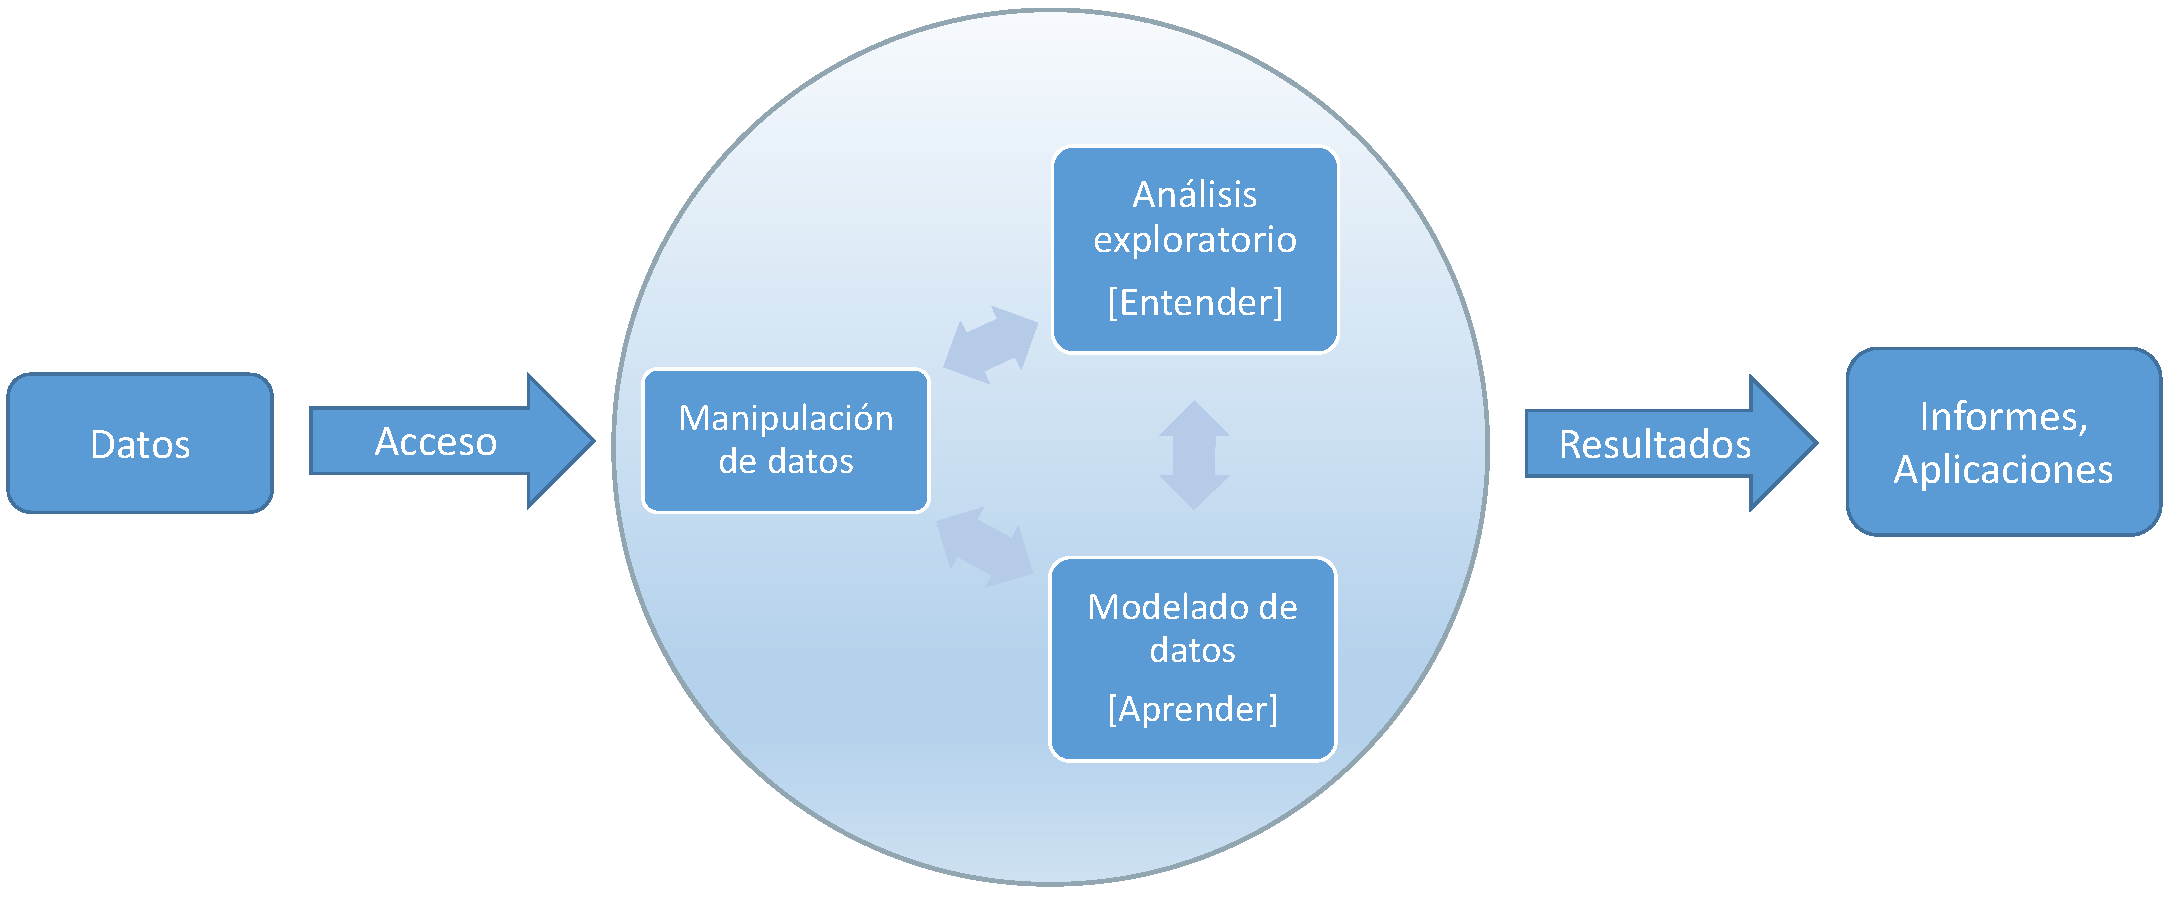
\includegraphics[width=0.7\linewidth]{figuras/esquema2} 

}

\caption{Etapas del proceso}\label{fig:esquema}
\end{figure}

\section{\texorpdfstring{El lenguaje y entorno estadístico
\texttt{R}}{El lenguaje y entorno estadístico R}}\label{el-lenguaje-y-entorno-estadistico-r}

\texttt{R} es un lenguaje de programación desarrollado específicamente
para el análisis estadístico y la visualización de datos.

\begin{itemize}
\item
  El lenguaje \texttt{R} es interpretado (similar a Matlab o Phyton)
  pero orientado al análisis estadístico (fórmulas modelos,
  factores,\ldots{}).

  \begin{itemize}
  \tightlist
  \item
    derivado del S (Laboratorios Bell).
  \end{itemize}
\item
  \texttt{R} es un \textbf{Software Libre} bajo las condiciones de
  licencia GPL de GNU, con código fuente de libre acceso.

  \begin{itemize}
  \tightlist
  \item
    Además de permitir crear \textbf{nuevas funciones}, se pueden
    examinar y modificar las ya existentes.
  \end{itemize}
\item
  Multiplataforma, disponible para los sistemas operativos más populares
  (Linux, Windows, MacOS X, \ldots{}).
\end{itemize}

\subsection{Principales
características}\label{principales-caracteristicas}

Se pueden destacar las siguientes características del entorno
\texttt{R}:

\begin{itemize}
\item
  Dispone de numerosos complementos (librerías, paquetes) que cubren
  ``literalmente'' todos los campos del análisis de datos.
\item
  Repositorios:

  \begin{itemize}
  \item
    \href{https://cran.r-project.org}{CRAN} (9705, 14972, \ldots{})
  \item
    \href{https://www.bioconductor.org}{Bioconductor} (1289, 1741,
    \ldots{}),
  \item
    \href{https://github.com/trending/r?since=monthly}{GitHub}, \ldots{}
  \end{itemize}
\item
  Existe una comunidad de usuarios (programadores) muy dinámica
  (multitud de paquetes adicionales).
\item
  Muy bien documentado y con numerosos foros de ayuda.
\item
  Puntos débiles (a priori): velocidad, memoria, \ldots{}
\end{itemize}

Aunque inicialmente fue un lenguaje desarrollado por estadísticos para
estadísticos:

\begin{figure}[!htb]

{\centering 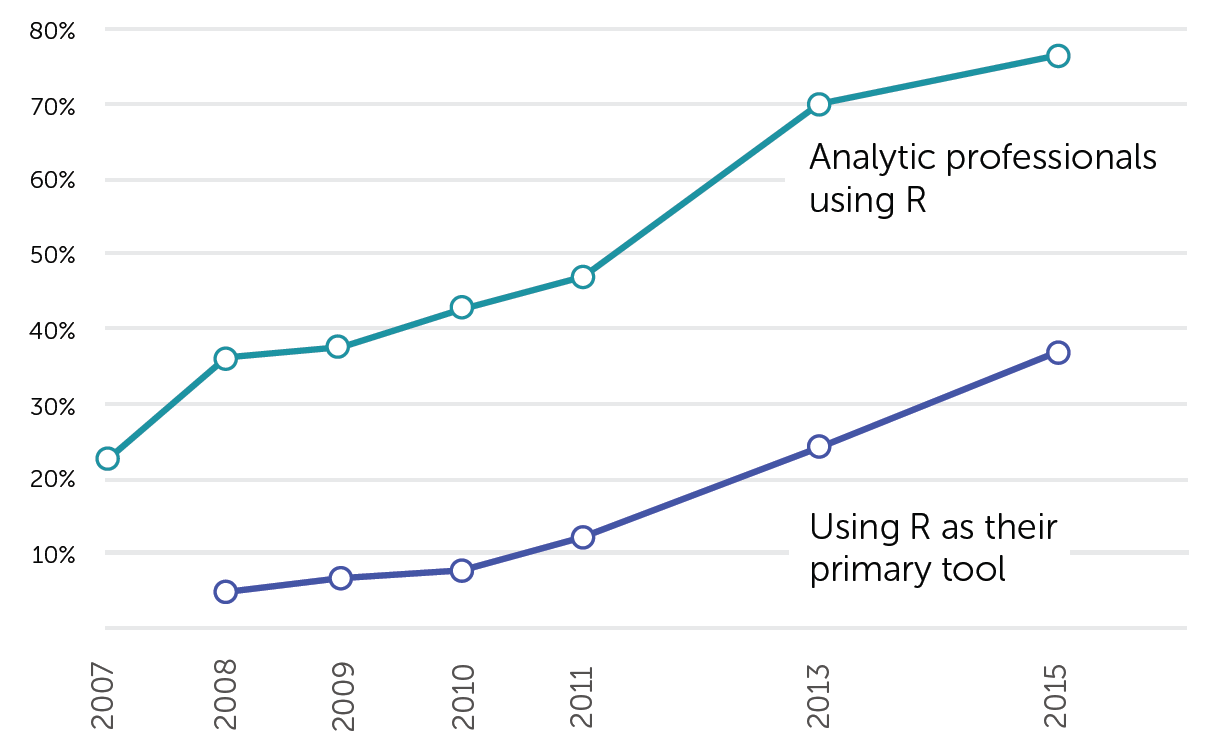
\includegraphics[width=0.4\linewidth]{figuras/rexer2016} 

}

\caption{Rexer Data Miner Survey 2007-2015}\label{fig:rexer}
\end{figure}

Hoy en día es muy popular:

\begin{figure}[!htb]

{\centering 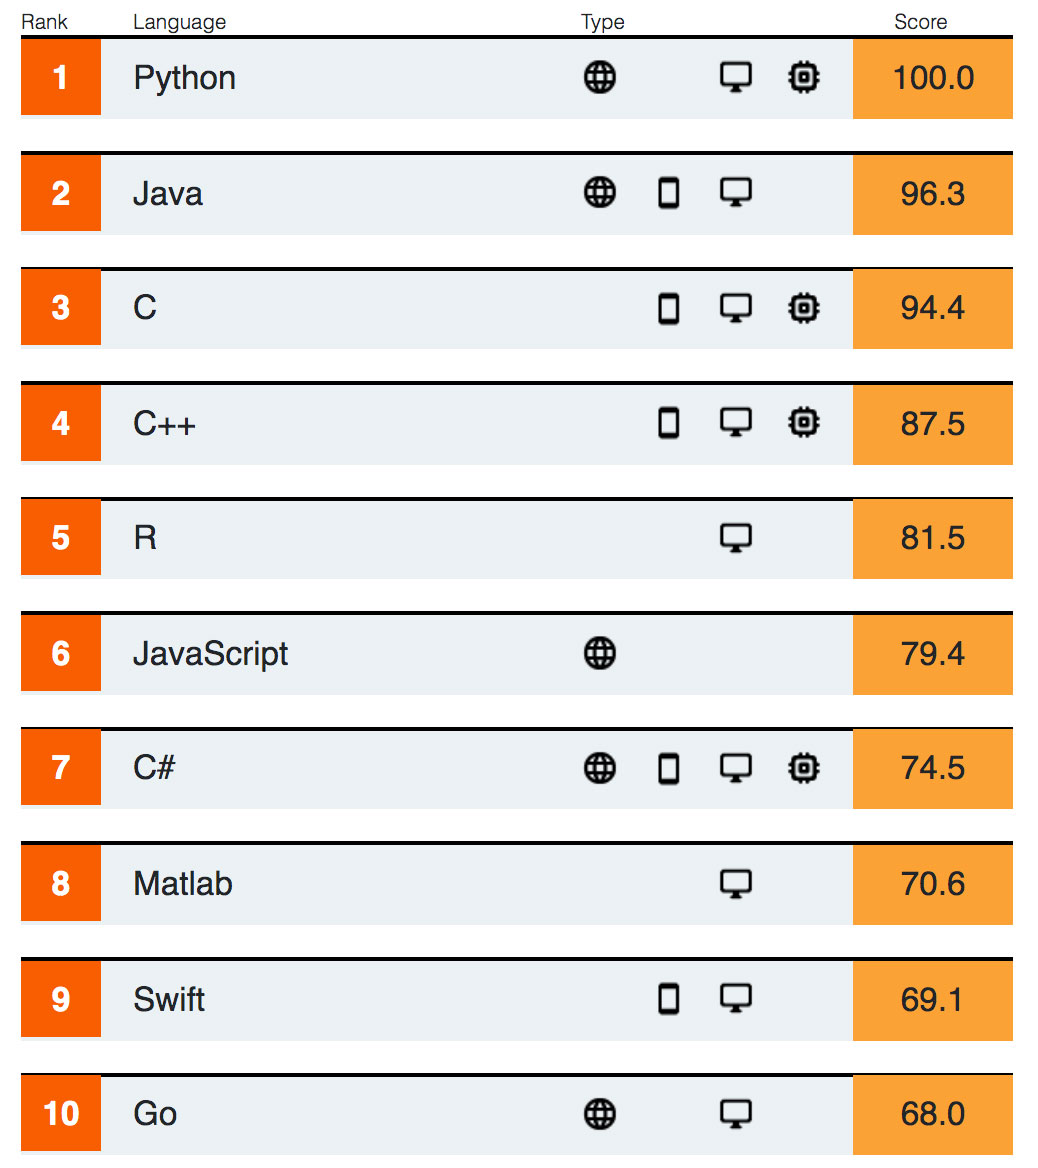
\includegraphics[width=0.35\linewidth]{figuras/IEEE-top-programming-languages-of-2019} 

}

\caption{[IEEE Spectrum](https://spectrum.ieee.org) Top Programming Languages, 2019}\label{fig:ieee}
\end{figure}

\texttt{R} destaca especialmente en:

\begin{itemize}
\item
  Representaciones gráficas.
\item
  Métodos estadísticos ``avanzados'':

  \begin{itemize}
  \item
    \emph{Data Science}: \emph{Statistical Learning}, \emph{Data
    Mining}, \emph{Machine Learning}, \emph{Business Intelligence},
    \ldots{}
  \item
    Datos funcionales.
  \item
    Estadística espacial.
  \item
    \ldots{}
  \end{itemize}
\item
  Análisis de datos ``complejos'':

  \begin{itemize}
  \item
    Big Data.
  \item
    Lenguaje natural (\emph{Text Mining}).
  \item
    Análisis de redes.
  \item
    \ldots{}
  \end{itemize}
\end{itemize}

\subsection{Interfaces gráficas}\label{interfaces-graficas}

El programa \texttt{R} utiliza una \textbf{interfaz de comandos} donde
se teclean las instrucciones que se pretenden ejecutar (ver Figura
\ref{fig:consola}).

Por ejemplo, para obtener una secuencia de números desde el 1 hasta el
10, se utilizará la sentencia:

\begin{Shaded}
\begin{Highlighting}[]
\DecValTok{1}\OperatorTok{:}\DecValTok{10}
\end{Highlighting}
\end{Shaded}

obteniéndose el resultado

\begin{verbatim}
##  [1]  1  2  3  4  5  6  7  8  9 10
\end{verbatim}

En el Apéndice \ref{instalacion} se detallan los pasos para la
instalación de \texttt{R}, y en el Apéndice \ref{interfaces} los de
otras interfaces gráficas.

\section{Entorno de trabajo}\label{entorno-de-trabajo}

\subsection{Ventana de Consola}\label{ventana-de-consola}

Al abrir el programa \texttt{R}, tal y como ya se ha visto, aparece la
siguiente ventana de consola para trabajar de modo interactivo en modo
comando (ver Figura \ref{fig:consola}).

\begin{figure}[!htb]

{\centering \includegraphics[width=0.7\linewidth]{figuras/consola} 

}

\caption{Consola de `R` en Windows (modo MDI).}\label{fig:consola}
\end{figure}

En la ventana de consola cada línea en que el usuario puede introducir
información se inicia con el carácter \texttt{\textgreater{}} que pone
el sistema \texttt{R}.

\begin{itemize}
\item
  Para ejecutar las instrucciones que están en una línea, se pulsa la
  tecla de Retorno (y por defecto se imprime el resultado).

\begin{Shaded}
\begin{Highlighting}[]
\DecValTok{2}\OperatorTok{+}\DecValTok{2}
\end{Highlighting}
\end{Shaded}

\begin{verbatim}
## [1] 4
\end{verbatim}

\begin{Shaded}
\begin{Highlighting}[]
\DecValTok{1}\OperatorTok{+}\DecValTok{2}\OperatorTok{*}\DecValTok{4}
\end{Highlighting}
\end{Shaded}

\begin{verbatim}
## [1] 9
\end{verbatim}
\item
  Se pueden escribir varias instrucción en una misma línea separándolas
  por ``;''

\begin{Shaded}
\begin{Highlighting}[]
\DecValTok{2}\OperatorTok{+}\DecValTok{2}\NormalTok{;}\DecValTok{1}\OperatorTok{+}\DecValTok{2}\OperatorTok{*}\DecValTok{4}
\end{Highlighting}
\end{Shaded}

\begin{verbatim}
## [1] 4
\end{verbatim}

\begin{verbatim}
## [1] 9
\end{verbatim}
\item
  Se pueden recuperar líneas de instrucciones introducidas anteriormente
  pulsando la tecla con la flecha ascendente del teclado, a fin de
  re-ejecutarlas o modificarlas.
\end{itemize}

\subsection{Ventana de Script}\label{ventana-de-script}

La ventana consola ejecuta de forma automática cada línea de comando.
Sin embargo, suele interesar guardar un conjunto de instrucciones en un
único archivo de texto para formar lo que se conoce como un
\emph{script}. Las instrucciones del script se copian y pegan en la
ventana de comandos para ser ejecutadas.

Para crear un fichero de script se selecciona el submenú \emph{Nuevo
script} dentro del menú \emph{Archivo}. Otra posibilidad es utilizar
directamente la combinación de teclas Ctrl+N.

\begin{figure}[!htb]

{\centering 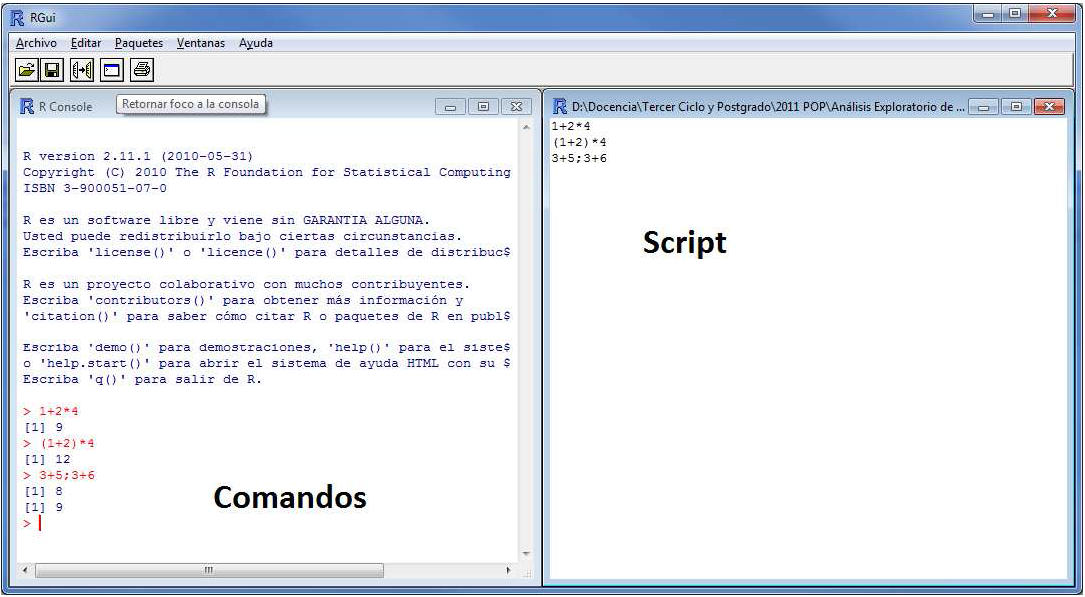
\includegraphics[width=0.7\linewidth]{figuras/script} 

}

\caption{Ventanas de la consola y de *script* en Windows (modo MDI).}\label{fig:script}
\end{figure}

Para guardar este tipo de fichero se utiliza directamente el menú
\emph{Archivo \textgreater{} Guardar como\ldots{}} y se elige a
continuación la ubicación en el disco duro del ordenador.

De igual modo para abrir un script existente se hace a través del menú
\emph{Archivo \textgreater{} Abrir script\ldots{}}.

En el Apéndice \ref{links} se incluyen enlaces a numerosos recursos para
el aprendizaje de R, incluyendo manuales y libros, además de otros
recursos para la obtención de ayuda.

\subsection{Ayuda dentro del programa}\label{ayuda-dentro-del-programa}

Como ya se ha comentado con anterioridad, hay manuales de \texttt{R}
alos que se puede acceder a través del menú \emph{Ayuda \textgreater{}
Manuales (en PDF)}

Puede empezarse utilizando \texttt{help.start()} o \texttt{demo()}.

Todas las funciones de \texttt{R} tienen su documentación integrada en
el programa. Para obtener la ayuda de una determinada función se
utilizará \texttt{help\ (función)} o de forma equivalente
\texttt{?función}.

Por ejemplo, la ayuda de la función \texttt{rnorm} (utilizada para la
generación de datos normales) se obtiene con el código

\begin{Shaded}
\begin{Highlighting}[]
\KeywordTok{help}\NormalTok{(rnorm)}
\NormalTok{?rnorm}
\end{Highlighting}
\end{Shaded}

En muchas ocasiones no se conoce el nombre exacto de la función de la
que queremos obtener la documentación. En estos casos, la función
\texttt{help.search()} realiza búsquedas en la documentación en todos
los paquetes instalados, estén cargados o no.

Por ejemplo, si no conocemos la función que permite calcular la mediana
de un conjunto de datos, se puede utilizar

\begin{Shaded}
\begin{Highlighting}[]
\KeywordTok{help.search}\NormalTok{(}\StringTok{"median"}\NormalTok{)}
\end{Highlighting}
\end{Shaded}

Para más detalles véase \texttt{?help.search}

\section{Librerías}\label{librerias}

\subsection{Paquetes}\label{paquetes}

Al iniciar el programa \texttt{R} se cargan por defecto una serie de
librerías básicas con las que se pueden realizar una gran cantidad de
operaciones básicas. Estas librerías conforman el llamado
\textbf{paquete base}.

En otras ocasiones es necesario cargar otras librerías distintas a las
anteriores. Esto se hace a través de los llamados paquetes (packages)
que pueden ser descargados directamente de la web

\url{http://cran.r-project.org/web/packages/}

o directamente a través del menú \texttt{Paquetes}.

\subsection{Instalación}\label{instalacion-pkg}

La instalación de un paquete, bajo el sistema operativo Windows, se
puede hacer de varias formas:

\begin{itemize}
\item
  Desde el menú \emph{Paquetes \textgreater{} Instalar
  paquete(s)\ldots{}}
\item
  Desde la ventana de consola utilizando la instrucción

\begin{Shaded}
\begin{Highlighting}[]
\KeywordTok{install.packages}\NormalTok{(}\StringTok{"nombre del paquete"}\NormalTok{)}
\end{Highlighting}
\end{Shaded}
\end{itemize}

Este proceso sólo es necesario realizarlo la primera vez que se utilice
el paquete.

\subsection{Carga}\label{carga}

Para utilizar un paquete ya instalado será necesario cargarlo, lo cual
se puede hacer de varias formas:

\begin{itemize}
\item
  Desde el menú \texttt{Paquetes\ \textgreater{}\ Cargar\ paquete(s)...}
\item
  Por consola, utilizando \texttt{library(nombre\ del\ paquete)}
\end{itemize}

Esta operación será necesario realizarla cada vez que se inicie una
sesión de R.

Finalmente, la ayuda de un paquete se puede obtener con la sentencia

\begin{Shaded}
\begin{Highlighting}[]
\KeywordTok{library}\NormalTok{(}\DataTypeTok{help =} \StringTok{"nombre del paquete"}\NormalTok{) }
\end{Highlighting}
\end{Shaded}

\section{Una primera sesión}\label{una-primera-sesion}

\subsection{Inicio de una sesión}\label{inicio-de-una-sesion}

El programa \texttt{R} (bajo Windows) se arranca al hacer un doble-click
sobre el icono del programa. Entonces aparecerá la ventana de consola
donde se escribirán los comandos y los resultados serán mostrados
inmediatamente por pantalla.

Veamos algún ejemplo:

\begin{Shaded}
\begin{Highlighting}[]
\DecValTok{3}\OperatorTok{+}\DecValTok{5}
\end{Highlighting}
\end{Shaded}

\begin{verbatim}
## [1] 8
\end{verbatim}

\begin{Shaded}
\begin{Highlighting}[]
\KeywordTok{sqrt}\NormalTok{(}\DecValTok{16}\NormalTok{) }\CommentTok{# raiz cuadrada de 16}
\end{Highlighting}
\end{Shaded}

\begin{verbatim}
## [1] 4
\end{verbatim}

\begin{Shaded}
\begin{Highlighting}[]
\NormalTok{pi }\CommentTok{# R reconoce el número pi}
\end{Highlighting}
\end{Shaded}

\begin{verbatim}
## [1] 3.141593
\end{verbatim}

Nótese que en los comandos se pueden hacer comentarios utilizando el
símbolo \texttt{\#}.

Los resultados obtenidos pueden guardarse en objetos. Por ejemplo, al
escribir

\begin{Shaded}
\begin{Highlighting}[]
\NormalTok{a <-}\StringTok{ }\DecValTok{3} \OperatorTok{+}\StringTok{ }\DecValTok{5}
\end{Highlighting}
\end{Shaded}

el resultado de la suma se guarda en \texttt{a}. Se puede comprobar si
la asignación se ha realizado correctamente escribiendo el nombre del
objeto

\begin{Shaded}
\begin{Highlighting}[]
\NormalTok{a}
\end{Highlighting}
\end{Shaded}

\begin{verbatim}
## [1] 8
\end{verbatim}

La asignación anterior se puede hacer del siguiente modo ejemplo, al
escribir

\begin{Shaded}
\begin{Highlighting}[]
\NormalTok{a <-}\StringTok{ }\DecValTok{3} \OperatorTok{+}\StringTok{ }\DecValTok{5}\NormalTok{; a}
\end{Highlighting}
\end{Shaded}

\begin{verbatim}
## [1] 8
\end{verbatim}

\textbf{Nota}: Habitualmente no habrá diferencia entre la utilización de
las asignaciones hechas con \texttt{=} y \texttt{\textless{}-} (aunque
nosotros emplearemos el segundo). Las diferencias aparecen a nivel de
programación y se tratarán en el Capítulo \ref{programacion}.

Veamos ahora un ejemplo un poco más avanzado. Con el siguiente código

\begin{itemize}
\item
  Se obtienen 200 datos simulados siguiendo una distribución gaussiana
  de media 105 y desviación típica 2
\item
  Se hace un resumen estadístico de los valores obtenidos
\item
  Se hace el correspondiente histograma y gráfico de cajas

\begin{Shaded}
\begin{Highlighting}[]
\NormalTok{x <-}\StringTok{ }\KeywordTok{rnorm}\NormalTok{(}\DataTypeTok{n =} \DecValTok{200}\NormalTok{, }\DataTypeTok{mean =} \DecValTok{105}\NormalTok{, }\DataTypeTok{sd =} \DecValTok{2}\NormalTok{) }\CommentTok{#datos normales}
\KeywordTok{summary}\NormalTok{(x) }\CommentTok{# resumen estadístico}
\end{Highlighting}
\end{Shaded}

\begin{verbatim}
##    Min. 1st Qu.  Median    Mean 3rd Qu.    Max. 
##   99.45  103.52  105.01  105.04  106.60  110.26
\end{verbatim}

\begin{Shaded}
\begin{Highlighting}[]
\KeywordTok{hist}\NormalTok{(x) }\CommentTok{# histograma}
\end{Highlighting}
\end{Shaded}

  \begin{center}\includegraphics[width=0.7\linewidth]{01-Introduccion_files/figure-latex/unnamed-chunk-14-1} \end{center}

\begin{Shaded}
\begin{Highlighting}[]
\KeywordTok{boxplot}\NormalTok{(x) }\CommentTok{# gráfico de cajas}
\end{Highlighting}
\end{Shaded}

  \begin{center}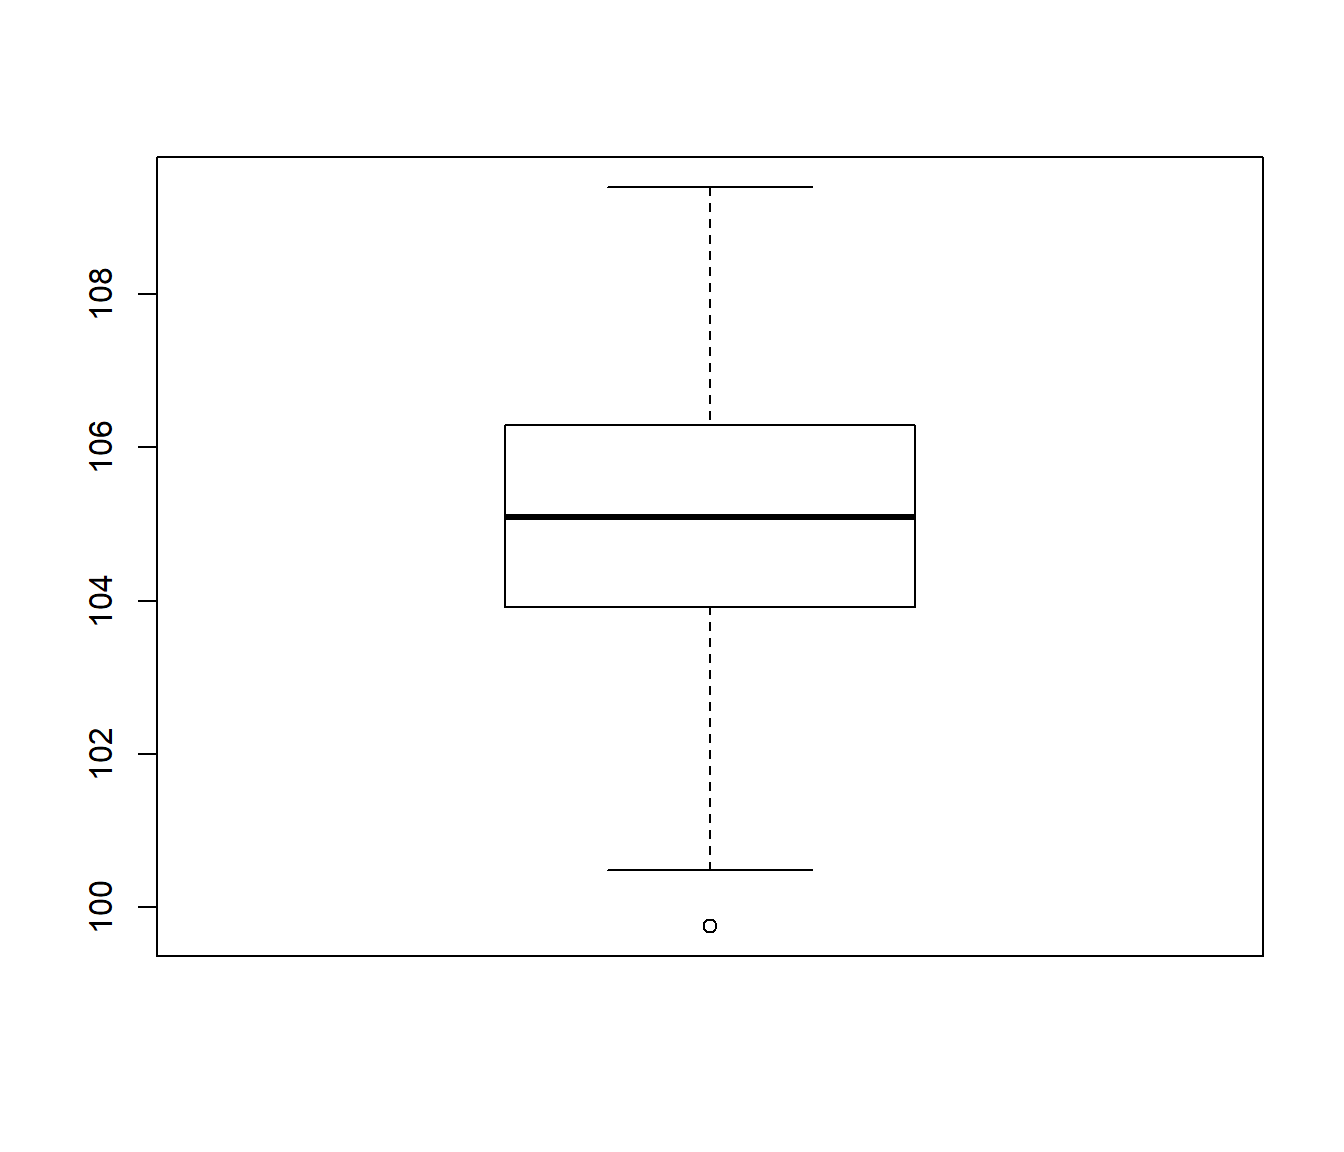
\includegraphics[width=0.7\linewidth]{01-Introduccion_files/figure-latex/unnamed-chunk-14-2} \end{center}
\end{itemize}

Es importante señalar que \texttt{R} diferencia entre mayúsculas y
minúsculas, de modo que los objetos \texttt{a} y \texttt{A} serán
diferentes.

\begin{Shaded}
\begin{Highlighting}[]
\NormalTok{a <-}\StringTok{ }\DecValTok{1}\OperatorTok{:}\DecValTok{10} \CommentTok{# secuencia de números}
\NormalTok{A <-}\StringTok{ "casa"}
\NormalTok{a}
\end{Highlighting}
\end{Shaded}

\begin{verbatim}
##  [1]  1  2  3  4  5  6  7  8  9 10
\end{verbatim}

\begin{Shaded}
\begin{Highlighting}[]
\NormalTok{A}
\end{Highlighting}
\end{Shaded}

\begin{verbatim}
## [1] "casa"
\end{verbatim}

\section{Objetos básicos}\label{objetos-basicos}

\texttt{R} es un lenguaje \textbf{orientado a objetos} lo que significa
que las variables, datos, funciones, resultados, etc., se guardan en la
memoria del ordenador en forma de \emph{objetos} con un nombre
específico.

Los principales tipos de valores básicos de \texttt{R} son:

\begin{itemize}
\item
  numéricos,
\item
  cadenas de caracteres, y
\item
  lógicos
\end{itemize}

\subsection{Objetos numéricos}\label{objetos-numericos}

Los valores numéricos adoptan la notación habitual en informática: punto
decimal, notacion científica, \ldots{}

\begin{Shaded}
\begin{Highlighting}[]
\NormalTok{pi}
\end{Highlighting}
\end{Shaded}

\begin{verbatim}
## [1] 3.141593
\end{verbatim}

\begin{Shaded}
\begin{Highlighting}[]
\FloatTok{1e3}
\end{Highlighting}
\end{Shaded}

\begin{verbatim}
## [1] 1000
\end{verbatim}

Con este tipo de objetos se pueden hacer operaciones aritméticas
utilizando el operador correspondiente.

\begin{Shaded}
\begin{Highlighting}[]
\NormalTok{a <-}\StringTok{ }\FloatTok{3.4}
\NormalTok{b <-}\StringTok{ }\FloatTok{4.5}
\NormalTok{a }\OperatorTok{*}\StringTok{ }\NormalTok{b}
\end{Highlighting}
\end{Shaded}

\begin{verbatim}
## [1] 15.3
\end{verbatim}

\begin{Shaded}
\begin{Highlighting}[]
\NormalTok{a }\OperatorTok{/}\StringTok{ }\NormalTok{b}
\end{Highlighting}
\end{Shaded}

\begin{verbatim}
## [1] 0.7555556
\end{verbatim}

\begin{Shaded}
\begin{Highlighting}[]
\NormalTok{a }\OperatorTok{+}\StringTok{ }\NormalTok{b}
\end{Highlighting}
\end{Shaded}

\begin{verbatim}
## [1] 7.9
\end{verbatim}

\begin{Shaded}
\begin{Highlighting}[]
\KeywordTok{min}\NormalTok{(a, b)}
\end{Highlighting}
\end{Shaded}

\begin{verbatim}
## [1] 3.4
\end{verbatim}

\subsection{Objetos tipo carácter}\label{objetos-tipo-caracter}

Las cadenas de caracteres se introducen delimitadas por comillas
(``nombre'') o por apóstrofos (`nombre').

\begin{Shaded}
\begin{Highlighting}[]
\NormalTok{a <-}\StringTok{ "casa grande"}
\NormalTok{a}
\end{Highlighting}
\end{Shaded}

\begin{verbatim}
## [1] "casa grande"
\end{verbatim}

\begin{Shaded}
\begin{Highlighting}[]
\NormalTok{a <-}\StringTok{ 'casa grande'}
\NormalTok{a}
\end{Highlighting}
\end{Shaded}

\begin{verbatim}
## [1] "casa grande"
\end{verbatim}

\begin{Shaded}
\begin{Highlighting}[]
\NormalTok{a <-}\StringTok{ 'casa "grande"'}
\NormalTok{a}
\end{Highlighting}
\end{Shaded}

\begin{verbatim}
## [1] "casa \"grande\""
\end{verbatim}

\subsection{Objetos lógicos}\label{objetos-logicos}

Los objetos lógicos sólo pueden tomar dos valores \texttt{TRUE}
(numéricamente toma el valor 1) y \texttt{FALSE} (valor 0).

\begin{Shaded}
\begin{Highlighting}[]
\NormalTok{A <-}\StringTok{ }\OtherTok{TRUE}
\NormalTok{B <-}\StringTok{ }\OtherTok{FALSE}
\NormalTok{A}
\end{Highlighting}
\end{Shaded}

\begin{verbatim}
## [1] TRUE
\end{verbatim}

\begin{Shaded}
\begin{Highlighting}[]
\NormalTok{B}
\end{Highlighting}
\end{Shaded}

\begin{verbatim}
## [1] FALSE
\end{verbatim}

\begin{Shaded}
\begin{Highlighting}[]
\CommentTok{# valores numéricos}
\KeywordTok{as.numeric}\NormalTok{(A)}
\end{Highlighting}
\end{Shaded}

\begin{verbatim}
## [1] 1
\end{verbatim}

\begin{Shaded}
\begin{Highlighting}[]
\KeywordTok{as.numeric}\NormalTok{(B)}
\end{Highlighting}
\end{Shaded}

\begin{verbatim}
## [1] 0
\end{verbatim}

\subsection{Operadores lógicos}\label{operadores-logicos}

Existen varios operadores en \texttt{R} que devuelven un valor de tipo
lógico. Veamos algún ejemplo

\begin{Shaded}
\begin{Highlighting}[]
\NormalTok{a <-}\StringTok{ }\DecValTok{2}
\NormalTok{b <-}\StringTok{ }\DecValTok{3}
\NormalTok{a }\OperatorTok{==}\StringTok{ }\NormalTok{b  }\CommentTok{# compara a y b}
\end{Highlighting}
\end{Shaded}

\begin{verbatim}
## [1] FALSE
\end{verbatim}

\begin{Shaded}
\begin{Highlighting}[]
\NormalTok{a }\OperatorTok{==}\StringTok{ }\NormalTok{a  }\CommentTok{# compara a y a}
\end{Highlighting}
\end{Shaded}

\begin{verbatim}
## [1] TRUE
\end{verbatim}

\begin{Shaded}
\begin{Highlighting}[]
\NormalTok{a }\OperatorTok{<}\StringTok{ }\NormalTok{b}
\end{Highlighting}
\end{Shaded}

\begin{verbatim}
## [1] TRUE
\end{verbatim}

\begin{Shaded}
\begin{Highlighting}[]
\NormalTok{b }\OperatorTok{<}\StringTok{ }\NormalTok{a}
\end{Highlighting}
\end{Shaded}

\begin{verbatim}
## [1] FALSE
\end{verbatim}

\begin{Shaded}
\begin{Highlighting}[]
\OperatorTok{!}\StringTok{ }\NormalTok{(b }\OperatorTok{<}\StringTok{ }\NormalTok{a) }\CommentTok{# ! niega la condición}
\end{Highlighting}
\end{Shaded}

\begin{verbatim}
## [1] TRUE
\end{verbatim}

\begin{Shaded}
\begin{Highlighting}[]
\DecValTok{2}\OperatorTok{**}\DecValTok{2} \OperatorTok{==}\StringTok{ }\DecValTok{2}\OperatorTok{^}\DecValTok{2}
\end{Highlighting}
\end{Shaded}

\begin{verbatim}
## [1] TRUE
\end{verbatim}

\begin{Shaded}
\begin{Highlighting}[]
\DecValTok{3}\OperatorTok{*}\DecValTok{2} \OperatorTok{==}\StringTok{ }\DecValTok{3}\OperatorTok{^}\DecValTok{2}
\end{Highlighting}
\end{Shaded}

\begin{verbatim}
## [1] FALSE
\end{verbatim}

Nótese la diferencia entre \texttt{=} (asignación) y \texttt{==}
(operador lógico)

\begin{Shaded}
\begin{Highlighting}[]
\DecValTok{2} \OperatorTok{==}\StringTok{ }\DecValTok{3}
\end{Highlighting}
\end{Shaded}

\begin{verbatim}
## [1] FALSE
\end{verbatim}

\begin{Shaded}
\begin{Highlighting}[]
\CommentTok{# 2 = 3 # produce un error:}
\CommentTok{# Error en 2 = 3 : lado izquierdo de la asignación inválida (do_set)}
\end{Highlighting}
\end{Shaded}

Se pueden encadenar varias condiciones lógicas utiilizando los
operadores \texttt{\&} (y lógico) y \texttt{\textbar{}} (o lógico).

\begin{Shaded}
\begin{Highlighting}[]
\OtherTok{TRUE} \OperatorTok{&}\StringTok{ }\OtherTok{TRUE}
\end{Highlighting}
\end{Shaded}

\begin{verbatim}
## [1] TRUE
\end{verbatim}

\begin{Shaded}
\begin{Highlighting}[]
\OtherTok{TRUE} \OperatorTok{|}\StringTok{ }\OtherTok{TRUE}
\end{Highlighting}
\end{Shaded}

\begin{verbatim}
## [1] TRUE
\end{verbatim}

\begin{Shaded}
\begin{Highlighting}[]
\OtherTok{TRUE} \OperatorTok{&}\StringTok{ }\OtherTok{FALSE}
\end{Highlighting}
\end{Shaded}

\begin{verbatim}
## [1] FALSE
\end{verbatim}

\begin{Shaded}
\begin{Highlighting}[]
\OtherTok{TRUE} \OperatorTok{|}\StringTok{ }\OtherTok{FALSE}
\end{Highlighting}
\end{Shaded}

\begin{verbatim}
## [1] TRUE
\end{verbatim}

\begin{Shaded}
\begin{Highlighting}[]
\DecValTok{2} \OperatorTok{<}\StringTok{ }\DecValTok{3} \OperatorTok{&}\StringTok{ }\DecValTok{3} \OperatorTok{<}\StringTok{ }\DecValTok{1}
\end{Highlighting}
\end{Shaded}

\begin{verbatim}
## [1] FALSE
\end{verbatim}

\begin{Shaded}
\begin{Highlighting}[]
\DecValTok{2} \OperatorTok{<}\StringTok{ }\DecValTok{3} \OperatorTok{|}\StringTok{ }\DecValTok{3} \OperatorTok{<}\StringTok{ }\DecValTok{1}
\end{Highlighting}
\end{Shaded}

\begin{verbatim}
## [1] TRUE
\end{verbatim}

\section{Área de trabajo}\label{area-de-trabajo}

Como ya se ha comentado con anterioridad es posible guardar los comandos
que se han utilizado en una sesión en ficheros llamados \textbf{script}.
En ocasiones interesará además guardar todos los objetos que han sido
generados a lo largo de una sesión de trabajo.

El \textbf{Workspace} o \textbf{Área de Trabajo} es el entorno en el que
se puede guardar todo el trabajo realizado en una sesión. De este modo,
la próxima vez que se inicie el programa, al cargar dicho entorno, se
podrá acceder a lo objetos almacenados en él.

En primer lugar, para saber los objetos que tenemos en memoria se
utiliza la función \texttt{ls}. Por ejemplo, supongamos que acabamos de
iniciar una sesión de \texttt{R} y hemos escrito

\begin{Shaded}
\begin{Highlighting}[]
\NormalTok{a <-}\StringTok{ }\DecValTok{1}\OperatorTok{:}\DecValTok{10}
\NormalTok{b <-}\StringTok{ }\KeywordTok{log}\NormalTok{(}\DecValTok{50}\NormalTok{)}
\end{Highlighting}
\end{Shaded}

Entonces al utilizar \texttt{ls} se obtendrá la siguiente lista de
objetos en memoria

\begin{Shaded}
\begin{Highlighting}[]
\KeywordTok{ls}\NormalTok{()}
\end{Highlighting}
\end{Shaded}

\begin{verbatim}
## [1] "a" "b"
\end{verbatim}

También es posible borrar objetos a través de la función \texttt{rm}

\begin{Shaded}
\begin{Highlighting}[]
\KeywordTok{rm}\NormalTok{(b)}
\KeywordTok{ls}\NormalTok{()}
\end{Highlighting}
\end{Shaded}

\begin{verbatim}
## [1] "a"
\end{verbatim}

Para borrar todos los objetos en memoria se puede utilizar
\texttt{rm(list=ls())}

\begin{Shaded}
\begin{Highlighting}[]
\KeywordTok{rm}\NormalTok{(}\DataTypeTok{list =} \KeywordTok{ls}\NormalTok{())}
\end{Highlighting}
\end{Shaded}

\begin{verbatim}
## character(0)
\end{verbatim}

\texttt{character(0)} (lista vacía) significa que no hay objetos en
memoria.

\subsection{Guardar y cargar
resultados}\label{guardar-y-cargar-resultados}

Para guardar el área de trabajo (Workspace) con todos los objetos de
memoria (es decir, los que figuran al utilizar \texttt{ls()}) se utiliza
la función \texttt{save.image(nombre\ archivo)}.

\begin{Shaded}
\begin{Highlighting}[]
\KeywordTok{rm}\NormalTok{(}\DataTypeTok{list =} \KeywordTok{ls}\NormalTok{()) }\CommentTok{# primero borramos toda la mamoria}
\NormalTok{x <-}\StringTok{ }\DecValTok{20}
\NormalTok{y <-}\StringTok{ }\DecValTok{34}
\NormalTok{z <-}\StringTok{ "casa"}
\KeywordTok{save.image}\NormalTok{(}\DataTypeTok{file =} \StringTok{"prueba.RData"}\NormalTok{) }\CommentTok{# guarda area de trabajo en prueba.RData}
\end{Highlighting}
\end{Shaded}

La función \texttt{save} permite guardar los objetos seleccionados.

\begin{Shaded}
\begin{Highlighting}[]
\KeywordTok{save}\NormalTok{(x, y, }\DataTypeTok{file =} \StringTok{"prueba2.RData"}\NormalTok{) }\CommentTok{# guarda los objetos x e y}
\end{Highlighting}
\end{Shaded}

Para cargar una ára de trabajo ya exitente se utiliza la función
\texttt{load()}.

\begin{Shaded}
\begin{Highlighting}[]
\KeywordTok{load}\NormalTok{(}\StringTok{"prueba2.RData"}\NormalTok{) }\CommentTok{# carga área de trabajo}
\end{Highlighting}
\end{Shaded}

\subsection{Directorio de trabajo}\label{directorio-de-trabajo}

Por defecto \texttt{R} utiliza una carpeta de trabajo donde guardará
toda la información. Dicha carpeta se puede obtener con la función

\begin{Shaded}
\begin{Highlighting}[]
\KeywordTok{getwd}\NormalTok{() }
\end{Highlighting}
\end{Shaded}

\begin{verbatim}
## [1] "d:/"
\end{verbatim}

El directorio de trabajo se puede cambiar utilizando
\texttt{setwd(carpeta)}. Por ejemplo, para cambiar el directorio de
trabajo a \texttt{c:\textbackslash{}datos}, se utiliza el comando

\begin{Shaded}
\begin{Highlighting}[]
\KeywordTok{setwd}\NormalTok{(}\StringTok{"c:/datos"}\NormalTok{)}
\CommentTok{# Importante la barra utilizada}
\CommentTok{# NO funciona setwd("c:\textbackslash{}datos")}
\end{Highlighting}
\end{Shaded}

\chapter{Estructuras de datos}\label{estructuras-de-datos}

En los ejemplos que hemos visto hasta ahora los objetos de \texttt{R}
almacenaban un único valor cada uno. Sin embargo, las estructuras de
datos que proporciona \texttt{R} permiten almacenar en un mismo objeto
varios valores. Las principales estructuras son:

\begin{itemize}
\item
  Vectores
\item
  Matrices y Arrays
\item
  Data Frames
\item
  Listas
\end{itemize}

\section{Vectores}\label{vectores}

Un vector es un conjunto de valores básicos del mismo tipo. La forma más
sencilla de crear vectores es a través de la función \texttt{c()} que se
usa para combinar (concatenar) valores.

\begin{Shaded}
\begin{Highlighting}[]
\NormalTok{x <-}\StringTok{ }\KeywordTok{c}\NormalTok{(}\DecValTok{3}\NormalTok{, }\DecValTok{5}\NormalTok{, }\DecValTok{7}\NormalTok{)}
\NormalTok{x}
\end{Highlighting}
\end{Shaded}

\begin{verbatim}
## [1] 3 5 7
\end{verbatim}

\begin{Shaded}
\begin{Highlighting}[]
\NormalTok{y <-}\StringTok{ }\KeywordTok{c}\NormalTok{(}\DecValTok{8}\NormalTok{, }\DecValTok{9}\NormalTok{)}
\NormalTok{y}
\end{Highlighting}
\end{Shaded}

\begin{verbatim}
## [1] 8 9
\end{verbatim}

\begin{Shaded}
\begin{Highlighting}[]
\KeywordTok{c}\NormalTok{(x, y)}
\end{Highlighting}
\end{Shaded}

\begin{verbatim}
## [1] 3 5 7 8 9
\end{verbatim}

\begin{Shaded}
\begin{Highlighting}[]
\NormalTok{z <-}\StringTok{ }\KeywordTok{c}\NormalTok{(}\StringTok{"Hola"}\NormalTok{, }\StringTok{"Adios"}\NormalTok{)}
\NormalTok{z}
\end{Highlighting}
\end{Shaded}

\begin{verbatim}
## [1] "Hola"  "Adios"
\end{verbatim}

\subsection{Generación de secuencias}\label{generacion-de-secuencias}

Existen varias funciones que pemiten obtener secuencias de números

\begin{Shaded}
\begin{Highlighting}[]
\NormalTok{x <-}\StringTok{ }\DecValTok{1}\OperatorTok{:}\DecValTok{5}
\NormalTok{x}
\end{Highlighting}
\end{Shaded}

\begin{verbatim}
## [1] 1 2 3 4 5
\end{verbatim}

\begin{Shaded}
\begin{Highlighting}[]
\KeywordTok{seq}\NormalTok{(}\DecValTok{1}\NormalTok{, }\DecValTok{5}\NormalTok{, }\FloatTok{0.5}\NormalTok{)}
\end{Highlighting}
\end{Shaded}

\begin{verbatim}
## [1] 1.0 1.5 2.0 2.5 3.0 3.5 4.0 4.5 5.0
\end{verbatim}

\begin{Shaded}
\begin{Highlighting}[]
\KeywordTok{seq}\NormalTok{(}\DataTypeTok{from=}\DecValTok{1}\NormalTok{, }\DataTypeTok{to=}\DecValTok{5}\NormalTok{, }\DataTypeTok{length=}\DecValTok{9}\NormalTok{)}
\end{Highlighting}
\end{Shaded}

\begin{verbatim}
## [1] 1.0 1.5 2.0 2.5 3.0 3.5 4.0 4.5 5.0
\end{verbatim}

\begin{Shaded}
\begin{Highlighting}[]
\KeywordTok{rep}\NormalTok{(}\DecValTok{1}\NormalTok{, }\DecValTok{5}\NormalTok{)}
\end{Highlighting}
\end{Shaded}

\begin{verbatim}
## [1] 1 1 1 1 1
\end{verbatim}

\subsection{Generación secuencias
aleatorias}\label{generacion-secuencias-aleatorias}

A continuación se obtiene una simulación de 10 lanzamientos de un dado

\begin{Shaded}
\begin{Highlighting}[]
\KeywordTok{sample}\NormalTok{(}\DecValTok{1}\OperatorTok{:}\DecValTok{6}\NormalTok{, }\DataTypeTok{size=}\DecValTok{10}\NormalTok{, }\DataTypeTok{replace =}\NormalTok{ T) }\CommentTok{#lanzamiento de un dado}
\end{Highlighting}
\end{Shaded}

\begin{verbatim}
##  [1] 1 1 5 5 4 5 1 2 3 1
\end{verbatim}

Para simular el lanzamiento de una moneda podemos escribir

\begin{Shaded}
\begin{Highlighting}[]
\NormalTok{resultado <-}\StringTok{ }\KeywordTok{c}\NormalTok{(}\DataTypeTok{cara=}\DecValTok{1}\NormalTok{,}\DataTypeTok{cruz=}\DecValTok{0}\NormalTok{) }\CommentTok{# se le han asignado nombres al objeto}
\KeywordTok{print}\NormalTok{(resultado)}
\end{Highlighting}
\end{Shaded}

\begin{verbatim}
## cara cruz 
##    1    0
\end{verbatim}

\begin{Shaded}
\begin{Highlighting}[]
\KeywordTok{class}\NormalTok{(resultado)}
\end{Highlighting}
\end{Shaded}

\begin{verbatim}
## [1] "numeric"
\end{verbatim}

\begin{Shaded}
\begin{Highlighting}[]
\KeywordTok{attributes}\NormalTok{(resultado)}
\end{Highlighting}
\end{Shaded}

\begin{verbatim}
## $names
## [1] "cara" "cruz"
\end{verbatim}

\begin{Shaded}
\begin{Highlighting}[]
\KeywordTok{names}\NormalTok{(resultado)}
\end{Highlighting}
\end{Shaded}

\begin{verbatim}
## [1] "cara" "cruz"
\end{verbatim}

\begin{Shaded}
\begin{Highlighting}[]
\NormalTok{lanz <-}\StringTok{ }\KeywordTok{sample}\NormalTok{(resultado, }\DataTypeTok{size=}\DecValTok{10}\NormalTok{, }\DataTypeTok{replace =}\NormalTok{ T)}
\NormalTok{lanz}
\end{Highlighting}
\end{Shaded}

\begin{verbatim}
## cruz cara cara cruz cara cruz cruz cruz cruz cara 
##    0    1    1    0    1    0    0    0    0    1
\end{verbatim}

\begin{Shaded}
\begin{Highlighting}[]
\KeywordTok{table}\NormalTok{(lanz)}
\end{Highlighting}
\end{Shaded}

\begin{verbatim}
## lanz
## 0 1 
## 6 4
\end{verbatim}

Otros ejemplos

\begin{Shaded}
\begin{Highlighting}[]
\KeywordTok{rnorm}\NormalTok{(}\DecValTok{10}\NormalTok{)  }\CommentTok{# rnorm(10, mean = 0, sd = 1)}
\end{Highlighting}
\end{Shaded}

\begin{verbatim}
##  [1]  0.5542825 -1.8587648 -0.4839736  0.2298712 -0.6344355 -0.4999402
##  [7]  0.2188108 -2.1008389  0.9892206  1.1516896
\end{verbatim}

\begin{Shaded}
\begin{Highlighting}[]
\KeywordTok{runif}\NormalTok{(}\DecValTok{15}\NormalTok{, }\DataTypeTok{min =} \DecValTok{2}\NormalTok{, }\DataTypeTok{max =} \DecValTok{10}\NormalTok{)}
\end{Highlighting}
\end{Shaded}

\begin{verbatim}
##  [1] 5.053462 3.457846 3.202863 7.908254 8.815679 2.484881 2.017832
##  [8] 4.345444 8.438295 9.233788 6.448266 9.304473 4.571463 9.549888
## [15] 9.240699
\end{verbatim}

El lector puede utilizar la función \texttt{help()} para obtener la
ayuda de las funciones anteriores.

\subsection{Selección de elementos de un
vector}\label{seleccion-de-elementos-de-un-vector}

Para acceder a los elementos de un vector se indica entre corchetes el
correspondiente vector de subíndices (enteros positivos).

\begin{Shaded}
\begin{Highlighting}[]
\NormalTok{x <-}\StringTok{ }\KeywordTok{seq}\NormalTok{(}\OperatorTok{-}\DecValTok{3}\NormalTok{, }\DecValTok{3}\NormalTok{, }\DecValTok{1}\NormalTok{)}
\NormalTok{x}
\end{Highlighting}
\end{Shaded}

\begin{verbatim}
## [1] -3 -2 -1  0  1  2  3
\end{verbatim}

\begin{Shaded}
\begin{Highlighting}[]
\NormalTok{x[}\DecValTok{1}\NormalTok{] }\CommentTok{# primer elemento}
\end{Highlighting}
\end{Shaded}

\begin{verbatim}
## [1] -3
\end{verbatim}

\begin{Shaded}
\begin{Highlighting}[]
\NormalTok{ii <-}\StringTok{ }\KeywordTok{c}\NormalTok{(}\DecValTok{1}\NormalTok{, }\DecValTok{5}\NormalTok{, }\DecValTok{7}\NormalTok{)}
\NormalTok{x[ii] }\CommentTok{#posiciones 1, 5 y 7}
\end{Highlighting}
\end{Shaded}

\begin{verbatim}
## [1] -3  1  3
\end{verbatim}

\begin{Shaded}
\begin{Highlighting}[]
\NormalTok{ii <-}\StringTok{ }\NormalTok{x}\OperatorTok{>}\DecValTok{0}\NormalTok{; ii}
\end{Highlighting}
\end{Shaded}

\begin{verbatim}
## [1] FALSE FALSE FALSE FALSE  TRUE  TRUE  TRUE
\end{verbatim}

\begin{Shaded}
\begin{Highlighting}[]
\NormalTok{x[ii]  }\CommentTok{# valores positivos}
\end{Highlighting}
\end{Shaded}

\begin{verbatim}
## [1] 1 2 3
\end{verbatim}

\begin{Shaded}
\begin{Highlighting}[]
\NormalTok{ii <-}\StringTok{ }\DecValTok{1}\OperatorTok{:}\DecValTok{3}
\NormalTok{x[}\OperatorTok{-}\NormalTok{ii]  }\CommentTok{# elementos de x salvo los 3 primeros}
\end{Highlighting}
\end{Shaded}

\begin{verbatim}
## [1] 0 1 2 3
\end{verbatim}

\subsection{Ordenación de vectores}\label{ordenacion-de-vectores}

\begin{Shaded}
\begin{Highlighting}[]
\NormalTok{x <-}\StringTok{ }\KeywordTok{c}\NormalTok{(}\DecValTok{65}\NormalTok{, }\DecValTok{18}\NormalTok{, }\DecValTok{59}\NormalTok{, }\DecValTok{18}\NormalTok{, }\DecValTok{6}\NormalTok{, }\DecValTok{94}\NormalTok{, }\DecValTok{26}\NormalTok{)}
\KeywordTok{sort}\NormalTok{(x)}
\end{Highlighting}
\end{Shaded}

\begin{verbatim}
## [1]  6 18 18 26 59 65 94
\end{verbatim}

\begin{Shaded}
\begin{Highlighting}[]
\KeywordTok{sort}\NormalTok{(x, }\DataTypeTok{decreasing =}\NormalTok{ T)}
\end{Highlighting}
\end{Shaded}

\begin{verbatim}
## [1] 94 65 59 26 18 18  6
\end{verbatim}

Otra posibilidad es utilizar un índice de ordenación.

\begin{Shaded}
\begin{Highlighting}[]
\NormalTok{ii <-}\StringTok{ }\KeywordTok{order}\NormalTok{(x)}
\NormalTok{ii  }\CommentTok{# índice de ordenación}
\end{Highlighting}
\end{Shaded}

\begin{verbatim}
## [1] 5 2 4 7 3 1 6
\end{verbatim}

\begin{Shaded}
\begin{Highlighting}[]
\NormalTok{x[ii]  }\CommentTok{# valores ordenados}
\end{Highlighting}
\end{Shaded}

\begin{verbatim}
## [1]  6 18 18 26 59 65 94
\end{verbatim}

La función \texttt{rev()} devuelve los valores del vector en orden
inverso.

\begin{Shaded}
\begin{Highlighting}[]
\KeywordTok{rev}\NormalTok{(x)}
\end{Highlighting}
\end{Shaded}

\begin{verbatim}
## [1] 26 94  6 18 59 18 65
\end{verbatim}

\subsection{Valores perdidos}\label{valores-perdidos}

Los valore perdidos aparecen normalmente cuando algún dato no ha sido
registrado. Este tipo de valores se registran como \texttt{NA}
(abreviatura de \emph{Not Available}).

Por ejemplo, supongamos que tenemos registrado las alturas de 5 personas
pero desconocemos la altura de la cuarta persona. El vector sería
registrado como sigue:

\begin{Shaded}
\begin{Highlighting}[]
\NormalTok{altura <-}\StringTok{ }\KeywordTok{c}\NormalTok{(}\DecValTok{165}\NormalTok{, }\DecValTok{178}\NormalTok{, }\DecValTok{184}\NormalTok{, }\OtherTok{NA}\NormalTok{, }\DecValTok{175}\NormalTok{)}
\NormalTok{altura}
\end{Highlighting}
\end{Shaded}

\begin{verbatim}
## [1] 165 178 184  NA 175
\end{verbatim}

Es importante notar que cualquier operación aritmética sobre un vector
que contiene algún \texttt{NA} dará como resultado otro \texttt{NA}.

\begin{Shaded}
\begin{Highlighting}[]
\KeywordTok{mean}\NormalTok{(altura)}
\end{Highlighting}
\end{Shaded}

\begin{verbatim}
## [1] NA
\end{verbatim}

Para forzar a \texttt{R} a que ignore los valores perdidos se utliza la
opción \texttt{na.rm\ =\ TRUE}.

\begin{Shaded}
\begin{Highlighting}[]
\KeywordTok{mean}\NormalTok{(altura, }\DataTypeTok{na.rm =} \OtherTok{TRUE}\NormalTok{)}
\end{Highlighting}
\end{Shaded}

\begin{verbatim}
## [1] 175.5
\end{verbatim}

\texttt{R} permite gestionar otros tipos de valores especiales:

\begin{itemize}
\item
  \texttt{NaN} (\emph{Not a Number}): es resultado de una
  indeterminación.
\item
  \texttt{Inf}: \texttt{R} representa valores no finitos \(\pm \infty\)
  como \texttt{Inf} y \texttt{-Inf}.
\end{itemize}

 \vspace*{0.3cm}

\begin{Shaded}
\begin{Highlighting}[]
\DecValTok{5}\OperatorTok{/}\DecValTok{0}  \CommentTok{# Infinito}
\end{Highlighting}
\end{Shaded}

\begin{verbatim}
## [1] Inf
\end{verbatim}

\begin{Shaded}
\begin{Highlighting}[]
\KeywordTok{log}\NormalTok{(}\DecValTok{0}\NormalTok{)  }\CommentTok{# -Infinito}
\end{Highlighting}
\end{Shaded}

\begin{verbatim}
## [1] -Inf
\end{verbatim}

\begin{Shaded}
\begin{Highlighting}[]
\DecValTok{0}\OperatorTok{/}\DecValTok{0}  \CommentTok{# Not a Number}
\end{Highlighting}
\end{Shaded}

\begin{verbatim}
## [1] NaN
\end{verbatim}

\subsection{Vectores no numéricos}\label{vectores-no-numericos}

Los vectores pueden ser no numéricos, aunque todas las componentes deben
ser del mismo tipo:

\begin{Shaded}
\begin{Highlighting}[]
\NormalTok{a <-}\StringTok{ }\KeywordTok{c}\NormalTok{(}\StringTok{"A Coruña"}\NormalTok{, }\StringTok{"Lugo"}\NormalTok{, }\StringTok{"Ourense"}\NormalTok{, }\StringTok{"Pontevedra"}\NormalTok{)}
\NormalTok{a}
\end{Highlighting}
\end{Shaded}

\begin{verbatim}
## [1] "A Coruña"   "Lugo"       "Ourense"    "Pontevedra"
\end{verbatim}

\begin{Shaded}
\begin{Highlighting}[]
\NormalTok{letters[}\DecValTok{1}\OperatorTok{:}\DecValTok{10}\NormalTok{]  }\CommentTok{# primeras 10 letas del abecedario}
\end{Highlighting}
\end{Shaded}

\begin{verbatim}
##  [1] "a" "b" "c" "d" "e" "f" "g" "h" "i" "j"
\end{verbatim}

\begin{Shaded}
\begin{Highlighting}[]
\NormalTok{LETTERS[}\DecValTok{1}\OperatorTok{:}\DecValTok{10}\NormalTok{]  }\CommentTok{# lo mismo en mayúscula}
\end{Highlighting}
\end{Shaded}

\begin{verbatim}
##  [1] "A" "B" "C" "D" "E" "F" "G" "H" "I" "J"
\end{verbatim}

\begin{Shaded}
\begin{Highlighting}[]
\NormalTok{month.name[}\DecValTok{1}\OperatorTok{:}\DecValTok{6}\NormalTok{]  }\CommentTok{# primeros 6 meses del año en inglés}
\end{Highlighting}
\end{Shaded}

\begin{verbatim}
## [1] "January"  "February" "March"    "April"    "May"      "June"
\end{verbatim}

\subsection{Factores}\label{factores}

Los factores se utilizan para representar datos categóricos. Se puede
pensar en ellos como vectores de enteros en los que cada entero tiene
asociada una etiqueta (\emph{label}). Los factores son muy importantes
en la modelización estadística ya que \texttt{R}los trata de forma
especial.

Utilizar factores con etiquetas es preferible a utilizar enteros porque
las etiquetas son auto-descriptivas.

Veamos un ejemplo. Supongamos que el vector \texttt{sexo} indica el sexo
de un persona codificado como 0 si hombre y 1 si mujer

\begin{Shaded}
\begin{Highlighting}[]
\NormalTok{sexo <-}\StringTok{ }\KeywordTok{c}\NormalTok{(}\DecValTok{0}\NormalTok{, }\DecValTok{1}\NormalTok{, }\DecValTok{1}\NormalTok{, }\DecValTok{1}\NormalTok{, }\DecValTok{0}\NormalTok{, }\DecValTok{0}\NormalTok{, }\DecValTok{1}\NormalTok{, }\DecValTok{0}\NormalTok{, }\DecValTok{1}\NormalTok{)}
\NormalTok{sexo}
\end{Highlighting}
\end{Shaded}

\begin{verbatim}
## [1] 0 1 1 1 0 0 1 0 1
\end{verbatim}

\begin{Shaded}
\begin{Highlighting}[]
\KeywordTok{table}\NormalTok{(sexo)}
\end{Highlighting}
\end{Shaded}

\begin{verbatim}
## sexo
## 0 1 
## 4 5
\end{verbatim}

El problema de introducir así los datos es que no queda reflejado la
etiquetación de los mismos. Para ello guardaremos los datos en una
estructura tipo factor:

\begin{Shaded}
\begin{Highlighting}[]
\NormalTok{sexo2 <-}\StringTok{ }\KeywordTok{factor}\NormalTok{(sexo, }\DataTypeTok{labels =} \KeywordTok{c}\NormalTok{(}\StringTok{"hombre"}\NormalTok{, }\StringTok{"mujer"}\NormalTok{)); sexo2}
\end{Highlighting}
\end{Shaded}

\begin{verbatim}
## [1] hombre mujer  mujer  mujer  hombre hombre mujer  hombre mujer 
## Levels: hombre mujer
\end{verbatim}

\begin{Shaded}
\begin{Highlighting}[]
\KeywordTok{levels}\NormalTok{(sexo2)  }\CommentTok{# devuelve los niveles de un factor}
\end{Highlighting}
\end{Shaded}

\begin{verbatim}
## [1] "hombre" "mujer"
\end{verbatim}

\begin{Shaded}
\begin{Highlighting}[]
\KeywordTok{unclass}\NormalTok{(sexo2)  }\CommentTok{# representación subyacente del factor}
\end{Highlighting}
\end{Shaded}

\begin{verbatim}
## [1] 1 2 2 2 1 1 2 1 2
## attr(,"levels")
## [1] "hombre" "mujer"
\end{verbatim}

\begin{Shaded}
\begin{Highlighting}[]
\KeywordTok{table}\NormalTok{(sexo2)}
\end{Highlighting}
\end{Shaded}

\begin{verbatim}
## sexo2
## hombre  mujer 
##      4      5
\end{verbatim}

Veamos otro ejemplo, en el que inicialmente tenemos datos categóricos.
Los niveles se toman automáticamente por orden alfabético

\begin{Shaded}
\begin{Highlighting}[]
\NormalTok{respuestas <-}\StringTok{ }\KeywordTok{factor}\NormalTok{(}\KeywordTok{c}\NormalTok{(}\StringTok{'si'}\NormalTok{, }\StringTok{'si'}\NormalTok{, }\StringTok{'no'}\NormalTok{, }\StringTok{'si'}\NormalTok{, }\StringTok{'si'}\NormalTok{, }\StringTok{'no'}\NormalTok{, }\StringTok{'no'}\NormalTok{))}
\NormalTok{respuestas}
\end{Highlighting}
\end{Shaded}

\begin{verbatim}
## [1] si si no si si no no
## Levels: no si
\end{verbatim}

Si deseásemos otro orden (lo cual puede ser importante en algunos casos,
por ejemplo para representaciones gráficas), habría que indicarlo
expresamente

\begin{Shaded}
\begin{Highlighting}[]
\NormalTok{respuestas <-}\StringTok{ }\KeywordTok{factor}\NormalTok{(}\KeywordTok{c}\NormalTok{(}\StringTok{'si'}\NormalTok{, }\StringTok{'si'}\NormalTok{, }\StringTok{'no'}\NormalTok{, }\StringTok{'si'}\NormalTok{, }\StringTok{'si'}\NormalTok{, }\StringTok{'no'}\NormalTok{, }\StringTok{'no'}\NormalTok{), }\DataTypeTok{levels =} \KeywordTok{c}\NormalTok{(}\StringTok{'si'}\NormalTok{, }\StringTok{'no'}\NormalTok{))}
\NormalTok{respuestas}
\end{Highlighting}
\end{Shaded}

\begin{verbatim}
## [1] si si no si si no no
## Levels: si no
\end{verbatim}

\section{Matrices y arrays}\label{matrices-y-arrays}

\subsection{Matrices}\label{matrices}

Las \emph{matrices} son la extensión natural de los vectores a dos
dimensiones. Su generalización a más dimensiones se llama \emph{array}.

Las matrices se pueden crear concatenando vectores con las funciones
\texttt{cbind} o \texttt{rbind}:

\begin{Shaded}
\begin{Highlighting}[]
\NormalTok{x <-}\StringTok{ }\KeywordTok{c}\NormalTok{(}\DecValTok{3}\NormalTok{, }\DecValTok{7}\NormalTok{, }\DecValTok{1}\NormalTok{, }\DecValTok{8}\NormalTok{, }\DecValTok{4}\NormalTok{)}
\NormalTok{y <-}\StringTok{ }\KeywordTok{c}\NormalTok{(}\DecValTok{7}\NormalTok{, }\DecValTok{5}\NormalTok{, }\DecValTok{2}\NormalTok{, }\DecValTok{1}\NormalTok{, }\DecValTok{0}\NormalTok{)}
\KeywordTok{cbind}\NormalTok{(x, y)  }\CommentTok{# por columnas}
\end{Highlighting}
\end{Shaded}

\begin{verbatim}
##      x y
## [1,] 3 7
## [2,] 7 5
## [3,] 1 2
## [4,] 8 1
## [5,] 4 0
\end{verbatim}

\begin{Shaded}
\begin{Highlighting}[]
\KeywordTok{rbind}\NormalTok{(x, y)  }\CommentTok{# por filas}
\end{Highlighting}
\end{Shaded}

\begin{verbatim}
##   [,1] [,2] [,3] [,4] [,5]
## x    3    7    1    8    4
## y    7    5    2    1    0
\end{verbatim}

Una matriz se puede crear con la función \texttt{matrix} donde el
parámetro \texttt{nrow} indica el número de filas y \texttt{ncol} el
número de columnas. Por defecto, los valores se colocan por columnas.

\begin{Shaded}
\begin{Highlighting}[]
\KeywordTok{matrix}\NormalTok{(}\DecValTok{1}\OperatorTok{:}\DecValTok{8}\NormalTok{, }\DataTypeTok{nrow =} \DecValTok{2}\NormalTok{, }\DataTypeTok{ncol =} \DecValTok{4}\NormalTok{)  }\CommentTok{# equivalente a matrix(1:8, nrow=2)}
\end{Highlighting}
\end{Shaded}

\begin{verbatim}
##      [,1] [,2] [,3] [,4]
## [1,]    1    3    5    7
## [2,]    2    4    6    8
\end{verbatim}

Los nombres de los parámetros se pueden acortar siempre y cuando no haya
ambigüedad, por lo que es habitual escribir

\begin{Shaded}
\begin{Highlighting}[]
\KeywordTok{matrix}\NormalTok{(}\DecValTok{1}\OperatorTok{:}\DecValTok{8}\NormalTok{, }\DataTypeTok{nr =} \DecValTok{2}\NormalTok{, }\DataTypeTok{nc =} \DecValTok{4}\NormalTok{)}
\end{Highlighting}
\end{Shaded}

\begin{verbatim}
##      [,1] [,2] [,3] [,4]
## [1,]    1    3    5    7
## [2,]    2    4    6    8
\end{verbatim}

Si queremos indicar que los valores se escriban por filas

\begin{Shaded}
\begin{Highlighting}[]
\KeywordTok{matrix}\NormalTok{(}\DecValTok{1}\OperatorTok{:}\DecValTok{8}\NormalTok{, }\DataTypeTok{nr =} \DecValTok{2}\NormalTok{, }\DataTypeTok{byrow =} \OtherTok{TRUE}\NormalTok{)}
\end{Highlighting}
\end{Shaded}

\begin{verbatim}
##      [,1] [,2] [,3] [,4]
## [1,]    1    2    3    4
## [2,]    5    6    7    8
\end{verbatim}

\subsection{Nombres en matrices}\label{nombres-en-matrices}

Se pueden dar nombres a las filas y columnas de una matriz.

\begin{Shaded}
\begin{Highlighting}[]
\NormalTok{x <-}\StringTok{ }\KeywordTok{matrix}\NormalTok{(}\KeywordTok{c}\NormalTok{(}\DecValTok{1}\NormalTok{, }\DecValTok{2}\NormalTok{, }\DecValTok{3}\NormalTok{, }\DecValTok{11}\NormalTok{, }\DecValTok{12}\NormalTok{, }\DecValTok{13}\NormalTok{), }\DataTypeTok{nrow =} \DecValTok{2}\NormalTok{, }\DataTypeTok{byrow =} \OtherTok{TRUE}\NormalTok{)}
\NormalTok{x}
\end{Highlighting}
\end{Shaded}

\begin{verbatim}
##      [,1] [,2] [,3]
## [1,]    1    2    3
## [2,]   11   12   13
\end{verbatim}

\begin{Shaded}
\begin{Highlighting}[]
\KeywordTok{rownames}\NormalTok{(x) <-}\StringTok{ }\KeywordTok{c}\NormalTok{(}\StringTok{"fila 1"}\NormalTok{, }\StringTok{"fila 2"}\NormalTok{)}
\KeywordTok{colnames}\NormalTok{(x) <-}\StringTok{ }\KeywordTok{c}\NormalTok{(}\StringTok{"col 1"}\NormalTok{, }\StringTok{"col 2"}\NormalTok{, }\StringTok{"col 3"}\NormalTok{)}
\NormalTok{x }
\end{Highlighting}
\end{Shaded}

\begin{verbatim}
##        col 1 col 2 col 3
## fila 1     1     2     3
## fila 2    11    12    13
\end{verbatim}

Obtenemos el mismo resultado si escribimos

\begin{Shaded}
\begin{Highlighting}[]
\KeywordTok{colnames}\NormalTok{(x) <-}\StringTok{ }\KeywordTok{paste}\NormalTok{(}\StringTok{"col"}\NormalTok{, }\DecValTok{1}\OperatorTok{:}\KeywordTok{ncol}\NormalTok{(x), }\DataTypeTok{sep=}\StringTok{" "}\NormalTok{)}
\end{Highlighting}
\end{Shaded}

Internamente, las matrices son vectores con un atributo especial: la
\emph{dimensión}.

\begin{Shaded}
\begin{Highlighting}[]
\KeywordTok{dim}\NormalTok{(x)}
\end{Highlighting}
\end{Shaded}

\begin{verbatim}
## [1] 2 3
\end{verbatim}

\begin{Shaded}
\begin{Highlighting}[]
\KeywordTok{attributes}\NormalTok{(x)}
\end{Highlighting}
\end{Shaded}

\begin{verbatim}
## $dim
## [1] 2 3
## 
## $dimnames
## $dimnames[[1]]
## [1] "fila 1" "fila 2"
## 
## $dimnames[[2]]
## [1] "col 1" "col 2" "col 3"
\end{verbatim}

\subsection{Acceso a los elementos de una
matriz}\label{acceso-a-los-elementos-de-una-matriz}

El acceso a los elementos de una matriz se realiza de forma análoga al
acceso ya comentado para los vectores.

\begin{Shaded}
\begin{Highlighting}[]
\NormalTok{x <-}\StringTok{ }\KeywordTok{matrix}\NormalTok{(}\DecValTok{1}\OperatorTok{:}\DecValTok{6}\NormalTok{, }\DecValTok{2}\NormalTok{, }\DecValTok{3}\NormalTok{); x}
\end{Highlighting}
\end{Shaded}

\begin{verbatim}
##      [,1] [,2] [,3]
## [1,]    1    3    5
## [2,]    2    4    6
\end{verbatim}

\begin{Shaded}
\begin{Highlighting}[]
\NormalTok{x[}\DecValTok{1}\NormalTok{, }\DecValTok{1}\NormalTok{]}
\end{Highlighting}
\end{Shaded}

\begin{verbatim}
## [1] 1
\end{verbatim}

\begin{Shaded}
\begin{Highlighting}[]
\NormalTok{x[}\DecValTok{2}\NormalTok{, }\DecValTok{2}\NormalTok{]}
\end{Highlighting}
\end{Shaded}

\begin{verbatim}
## [1] 4
\end{verbatim}

\begin{Shaded}
\begin{Highlighting}[]
\NormalTok{x[}\DecValTok{2}\NormalTok{, ]  }\CommentTok{# segunda fila}
\end{Highlighting}
\end{Shaded}

\begin{verbatim}
## [1] 2 4 6
\end{verbatim}

\begin{Shaded}
\begin{Highlighting}[]
\NormalTok{x[ ,}\DecValTok{2}\NormalTok{]  }\CommentTok{# segunda columna}
\end{Highlighting}
\end{Shaded}

\begin{verbatim}
## [1] 3 4
\end{verbatim}

\begin{Shaded}
\begin{Highlighting}[]
\NormalTok{x[}\DecValTok{1}\NormalTok{, }\DecValTok{1}\OperatorTok{:}\DecValTok{2}\NormalTok{]  }\CommentTok{# primera fila, columnas 1ª y 2ª }
\end{Highlighting}
\end{Shaded}

\begin{verbatim}
## [1] 1 3
\end{verbatim}

\subsection{Ordenación por filas y
columnas}\label{ordenacion-por-filas-y-columnas}

En ocasiones, interesará ordenar los elementos de una matriz por los
valores de una determinada columna o fila.

Por ejemplo, supongamos la matriz

\begin{Shaded}
\begin{Highlighting}[]
\NormalTok{x <-}\StringTok{ }\KeywordTok{c}\NormalTok{(}\DecValTok{79}\NormalTok{, }\DecValTok{100}\NormalTok{, }\DecValTok{116}\NormalTok{, }\DecValTok{121}\NormalTok{, }\DecValTok{52}\NormalTok{, }\DecValTok{134}\NormalTok{, }\DecValTok{123}\NormalTok{, }\DecValTok{109}\NormalTok{, }\DecValTok{80}\NormalTok{, }\DecValTok{107}\NormalTok{, }\DecValTok{66}\NormalTok{, }\DecValTok{118}\NormalTok{)}
\NormalTok{x <-}\StringTok{ }\KeywordTok{matrix}\NormalTok{(x, }\DataTypeTok{ncol=}\DecValTok{4}\NormalTok{, }\DataTypeTok{byrow=}\NormalTok{T); x}
\end{Highlighting}
\end{Shaded}

\begin{verbatim}
##      [,1] [,2] [,3] [,4]
## [1,]   79  100  116  121
## [2,]   52  134  123  109
## [3,]   80  107   66  118
\end{verbatim}

La matriz ordenada por los valores de la primera columna viene dada por

\begin{Shaded}
\begin{Highlighting}[]
\NormalTok{ii <-}\StringTok{ }\KeywordTok{order}\NormalTok{(x[ ,}\DecValTok{1}\NormalTok{])}
\NormalTok{x[ii, ]  }\CommentTok{# ordenación columna 1}
\end{Highlighting}
\end{Shaded}

\begin{verbatim}
##      [,1] [,2] [,3] [,4]
## [1,]   52  134  123  109
## [2,]   79  100  116  121
## [3,]   80  107   66  118
\end{verbatim}

De igual modo, si queremos ordenar por los valores de la cuarta columna:

\begin{Shaded}
\begin{Highlighting}[]
\NormalTok{ii <-}\StringTok{ }\KeywordTok{order}\NormalTok{(x[ ,}\DecValTok{4}\NormalTok{]); x[ii, ]  }\CommentTok{# ordenación columna 4}
\end{Highlighting}
\end{Shaded}

\begin{verbatim}
##      [,1] [,2] [,3] [,4]
## [1,]   52  134  123  109
## [2,]   80  107   66  118
## [3,]   79  100  116  121
\end{verbatim}

\subsection{Operaciones con Matrices y
Arrays}\label{operaciones-con-matrices-y-arrays}

A continuación se muestran algunas funciones que se pueden emplear con
matrices

\begin{longtable}[]{@{}ll@{}}
\toprule
Función & Descripción\tabularnewline
\midrule
\endhead
\texttt{dim(),nrow(),ncol()} & número de filas y/o
columnas\tabularnewline
\texttt{diag()} & diagonal de una matrix\tabularnewline
\texttt{*} & multiplicación elemento a elemento\tabularnewline
\texttt{\%*\%} & multiplicación matricial de matrices\tabularnewline
\texttt{cbind(),rbind()} & encadenamiento de columnas o
filas\tabularnewline
\texttt{t()} & transpuesta\tabularnewline
\texttt{solve(A)} & inversa de la matriz A\tabularnewline
\texttt{solve(A,b)} & solución del sistema de ecuaciones
\(Ax=b\)\tabularnewline
\texttt{qr()} & descomposición de Cholesky\tabularnewline
\texttt{eigen()} & autovalores y autovectores\tabularnewline
\texttt{svd()} & descomposición singular\tabularnewline
\bottomrule
\end{longtable}

\subsection{Ejemplos}\label{ejemplos}

\begin{Shaded}
\begin{Highlighting}[]
\NormalTok{x <-}\StringTok{ }\KeywordTok{matrix}\NormalTok{(}\DecValTok{1}\OperatorTok{:}\DecValTok{6}\NormalTok{, }\DataTypeTok{ncol =} \DecValTok{3}\NormalTok{)}
\NormalTok{x}
\end{Highlighting}
\end{Shaded}

\begin{verbatim}
##      [,1] [,2] [,3]
## [1,]    1    3    5
## [2,]    2    4    6
\end{verbatim}

\begin{Shaded}
\begin{Highlighting}[]
\KeywordTok{t}\NormalTok{(x)  }\CommentTok{# matriz transpuesta}
\end{Highlighting}
\end{Shaded}

\begin{verbatim}
##      [,1] [,2]
## [1,]    1    2
## [2,]    3    4
## [3,]    5    6
\end{verbatim}

\begin{Shaded}
\begin{Highlighting}[]
\KeywordTok{dim}\NormalTok{(x)  }\CommentTok{# dimensiones de la matriz}
\end{Highlighting}
\end{Shaded}

\begin{verbatim}
## [1] 2 3
\end{verbatim}

\subsection{Inversión de una matriz}\label{inversion-de-una-matriz}

\begin{Shaded}
\begin{Highlighting}[]
\NormalTok{A <-}\StringTok{ }\KeywordTok{matrix}\NormalTok{(}\KeywordTok{c}\NormalTok{(}\DecValTok{2}\NormalTok{, }\DecValTok{4}\NormalTok{, }\DecValTok{0}\NormalTok{, }\DecValTok{2}\NormalTok{), }\DataTypeTok{nrow =} \DecValTok{2}\NormalTok{); A}
\end{Highlighting}
\end{Shaded}

\begin{verbatim}
##      [,1] [,2]
## [1,]    2    0
## [2,]    4    2
\end{verbatim}

\begin{Shaded}
\begin{Highlighting}[]
\NormalTok{B <-}\StringTok{ }\KeywordTok{solve}\NormalTok{(A)}
\NormalTok{B  }\CommentTok{# inversa}
\end{Highlighting}
\end{Shaded}

\begin{verbatim}
##      [,1] [,2]
## [1,]  0.5  0.0
## [2,] -1.0  0.5
\end{verbatim}

\begin{Shaded}
\begin{Highlighting}[]
\NormalTok{A }\OperatorTok\StringTok{ }\NormalTok{B  }\CommentTok{# comprobamos que está bien}
\end{Highlighting}
\end{Shaded}

\begin{verbatim}
##      [,1] [,2]
## [1,]    1    0
## [2,]    0    1
\end{verbatim}

\section{Data frames}\label{data-frames}

Los \texttt{data.fames} (\emph{marcos de datos}) son el objeto más
habitual para el almacenamiento de datos. En este tipo de objetos cada
individuo de la muestra se corresponde con una fila y cada una de las
variables con una columna. Para la creación de estas estructuras se
utiliza la función \texttt{data.frame()}.

Este tipo de estructuras son en apariencia muy similares a las matrices,
con la ventaja de que permiten que los valores de las distintas columnas
sean de tipos diferentes. Por ejemplo, supongamos que tenemos
registrados los siguientes valores

\begin{Shaded}
\begin{Highlighting}[]
\NormalTok{Producto <-}\StringTok{ }\KeywordTok{c}\NormalTok{(}\StringTok{"Zumo"}\NormalTok{, }\StringTok{"Queso"}\NormalTok{, }\StringTok{"Yogourt"}\NormalTok{)}
\NormalTok{Seccion <-}\StringTok{ }\KeywordTok{c}\NormalTok{(}\StringTok{"Bebidas"}\NormalTok{, }\StringTok{"Lácteos"}\NormalTok{, }\StringTok{"Lácteos"}\NormalTok{)}
\NormalTok{Unidades <-}\StringTok{ }\KeywordTok{c}\NormalTok{(}\DecValTok{2}\NormalTok{, }\DecValTok{1}\NormalTok{, }\DecValTok{10}\NormalTok{)}
\end{Highlighting}
\end{Shaded}

Los valores anteriores se podrían guardar en una única matriz

\begin{Shaded}
\begin{Highlighting}[]
\NormalTok{x <-}\StringTok{ }\KeywordTok{cbind}\NormalTok{(Producto, Seccion, Unidades)}
\KeywordTok{class}\NormalTok{(x)}
\end{Highlighting}
\end{Shaded}

\begin{verbatim}
## [1] "matrix"
\end{verbatim}

\begin{Shaded}
\begin{Highlighting}[]
\NormalTok{x}
\end{Highlighting}
\end{Shaded}

\begin{verbatim}
##      Producto  Seccion   Unidades
## [1,] "Zumo"    "Bebidas" "2"     
## [2,] "Queso"   "Lácteos" "1"     
## [3,] "Yogourt" "Lácteos" "10"
\end{verbatim}

Sin embargo, el resultado anterior no es satisfactorio ya que todos los
valores se han transformado en caracteres. Una solución mejor es
utilizar un \texttt{data.frame}, con lo cual se mantiene el tipo
original de las variables.

\begin{Shaded}
\begin{Highlighting}[]
\NormalTok{lista.compra <-}\StringTok{ }\KeywordTok{data.frame}\NormalTok{(Producto, Seccion, Unidades)}
\KeywordTok{class}\NormalTok{(lista.compra)}
\end{Highlighting}
\end{Shaded}

\begin{verbatim}
## [1] "data.frame"
\end{verbatim}

\begin{Shaded}
\begin{Highlighting}[]
\NormalTok{lista.compra}
\end{Highlighting}
\end{Shaded}

\begin{verbatim}
##   Producto Seccion Unidades
## 1     Zumo Bebidas        2
## 2    Queso Lácteos        1
## 3  Yogourt Lácteos       10
\end{verbatim}

A continuación se muestran ejemplos que ilustran la manera de acceder a
los valores de un data.frame.

\begin{Shaded}
\begin{Highlighting}[]
\NormalTok{lista.compra}\OperatorTok{$}\NormalTok{Unidades}
\end{Highlighting}
\end{Shaded}

\begin{verbatim}
## [1]  2  1 10
\end{verbatim}

\begin{Shaded}
\begin{Highlighting}[]
\NormalTok{lista.compra[ ,}\DecValTok{3}\NormalTok{]  }\CommentTok{# de manera equivalente}
\end{Highlighting}
\end{Shaded}

\begin{verbatim}
## [1]  2  1 10
\end{verbatim}

\begin{Shaded}
\begin{Highlighting}[]
\NormalTok{lista.compra}\OperatorTok{$}\NormalTok{Seccion}
\end{Highlighting}
\end{Shaded}

\begin{verbatim}
## [1] Bebidas Lácteos Lácteos
## Levels: Bebidas Lácteos
\end{verbatim}

\begin{Shaded}
\begin{Highlighting}[]
\NormalTok{lista.compra}\OperatorTok{$}\NormalTok{Unidades[}\DecValTok{1}\OperatorTok{:}\DecValTok{2}\NormalTok{]  }\CommentTok{# primeros dos valores de Unidades}
\end{Highlighting}
\end{Shaded}

\begin{verbatim}
## [1] 2 1
\end{verbatim}

\begin{Shaded}
\begin{Highlighting}[]
\NormalTok{lista.compra[}\DecValTok{2}\NormalTok{,]  }\CommentTok{# segunda fila}
\end{Highlighting}
\end{Shaded}

\begin{verbatim}
##   Producto Seccion Unidades
## 2    Queso Lácteos        1
\end{verbatim}

La función \texttt{summary()} permite hacer un resumen estadístico de
las variables (columnas) del data.frame.

\begin{Shaded}
\begin{Highlighting}[]
\KeywordTok{summary}\NormalTok{(lista.compra)}
\end{Highlighting}
\end{Shaded}

\begin{verbatim}
##     Producto    Seccion     Unidades     
##  Queso  :1   Bebidas:1   Min.   : 1.000  
##  Yogourt:1   Lácteos:2   1st Qu.: 1.500  
##  Zumo   :1               Median : 2.000  
##                          Mean   : 4.333  
##                          3rd Qu.: 6.000  
##                          Max.   :10.000
\end{verbatim}

\section{Listas}\label{listas}

Las listas son colecciones ordenadas de cualquier tipo de objetos (en
\texttt{R} las listas son un tipo especial de vectores). Así, mientras
que los elementos de los vectores, matrices y arrays deben ser del mismo
tipo, en el caso de las listas se pueden tener elementos de tipos
distintos.

\begin{Shaded}
\begin{Highlighting}[]
\NormalTok{x <-}\StringTok{ }\KeywordTok{c}\NormalTok{(}\DecValTok{1}\NormalTok{, }\DecValTok{2}\NormalTok{, }\DecValTok{3}\NormalTok{, }\DecValTok{4}\NormalTok{)}
\NormalTok{y <-}\StringTok{ }\KeywordTok{c}\NormalTok{(}\StringTok{"Hombre"}\NormalTok{, }\StringTok{"Mujer"}\NormalTok{)}
\NormalTok{z <-}\StringTok{ }\KeywordTok{matrix}\NormalTok{(}\DecValTok{1}\OperatorTok{:}\DecValTok{12}\NormalTok{, }\DataTypeTok{ncol =} \DecValTok{4}\NormalTok{)}
\NormalTok{datos <-}\StringTok{ }\KeywordTok{list}\NormalTok{(}\DataTypeTok{A=}\NormalTok{x, }\DataTypeTok{B=}\NormalTok{y, }\DataTypeTok{C=}\NormalTok{z)}
\NormalTok{datos}
\end{Highlighting}
\end{Shaded}

\begin{verbatim}
## $A
## [1] 1 2 3 4
## 
## $B
## [1] "Hombre" "Mujer" 
## 
## $C
##      [,1] [,2] [,3] [,4]
## [1,]    1    4    7   10
## [2,]    2    5    8   11
## [3,]    3    6    9   12
\end{verbatim}

\chapter{Gráficos}\label{graficos}

\texttt{R} dispone de varias funciones que permiten la realización de
gráficos. Estas funciones se dividen en dos grandes grupos

\begin{itemize}
\item
  Gráficos de \textbf{alto nivel}: Crean un gráfico nuevo.

  \begin{itemize}
  \tightlist
  \item
    \texttt{plot,\ hist,\ boxplot,\ ...}
  \end{itemize}
\item
  Gráficos de \textbf{bajo nivel}: Permiten añadir elementos (líneas,
  puntos, \ldots{}) a un gráfico ya existente

  \begin{itemize}
  \item
    \texttt{points,\ lines,\ legend,\ text,\ ...}
  \item
    El parámetro \texttt{add=TRUE} convierte una función de nivel alto a
    bajo.
  \end{itemize}
\end{itemize}

Dentro de las funciones gráficas de alto nivel destaca la función
\texttt{plot} que tiene muchas variantes y dependiendo del tipo de datos
que se le pasen como argumento actuará de modo distinto.

\section{El comando plot}\label{el-comando-plot}

Si escribimos \texttt{plot(x,\ y)} donde \texttt{x} e \texttt{y} son
vectores, entonces \texttt{R} hará directamente el conocido como
\textbf{gráfico de dispersión} que representa en un sistema coordenado
los pares de valores \((x,y)\).

Por ejemplo, utilizando el siguiente código

\begin{Shaded}
\begin{Highlighting}[]
\KeywordTok{data}\NormalTok{(cars)}
\KeywordTok{plot}\NormalTok{(cars}\OperatorTok{$}\NormalTok{speed, cars}\OperatorTok{$}\NormalTok{dist)    }\CommentTok{# otra posibilidad plot(cars)}
\end{Highlighting}
\end{Shaded}

\begin{figure}[!htb]

{\centering 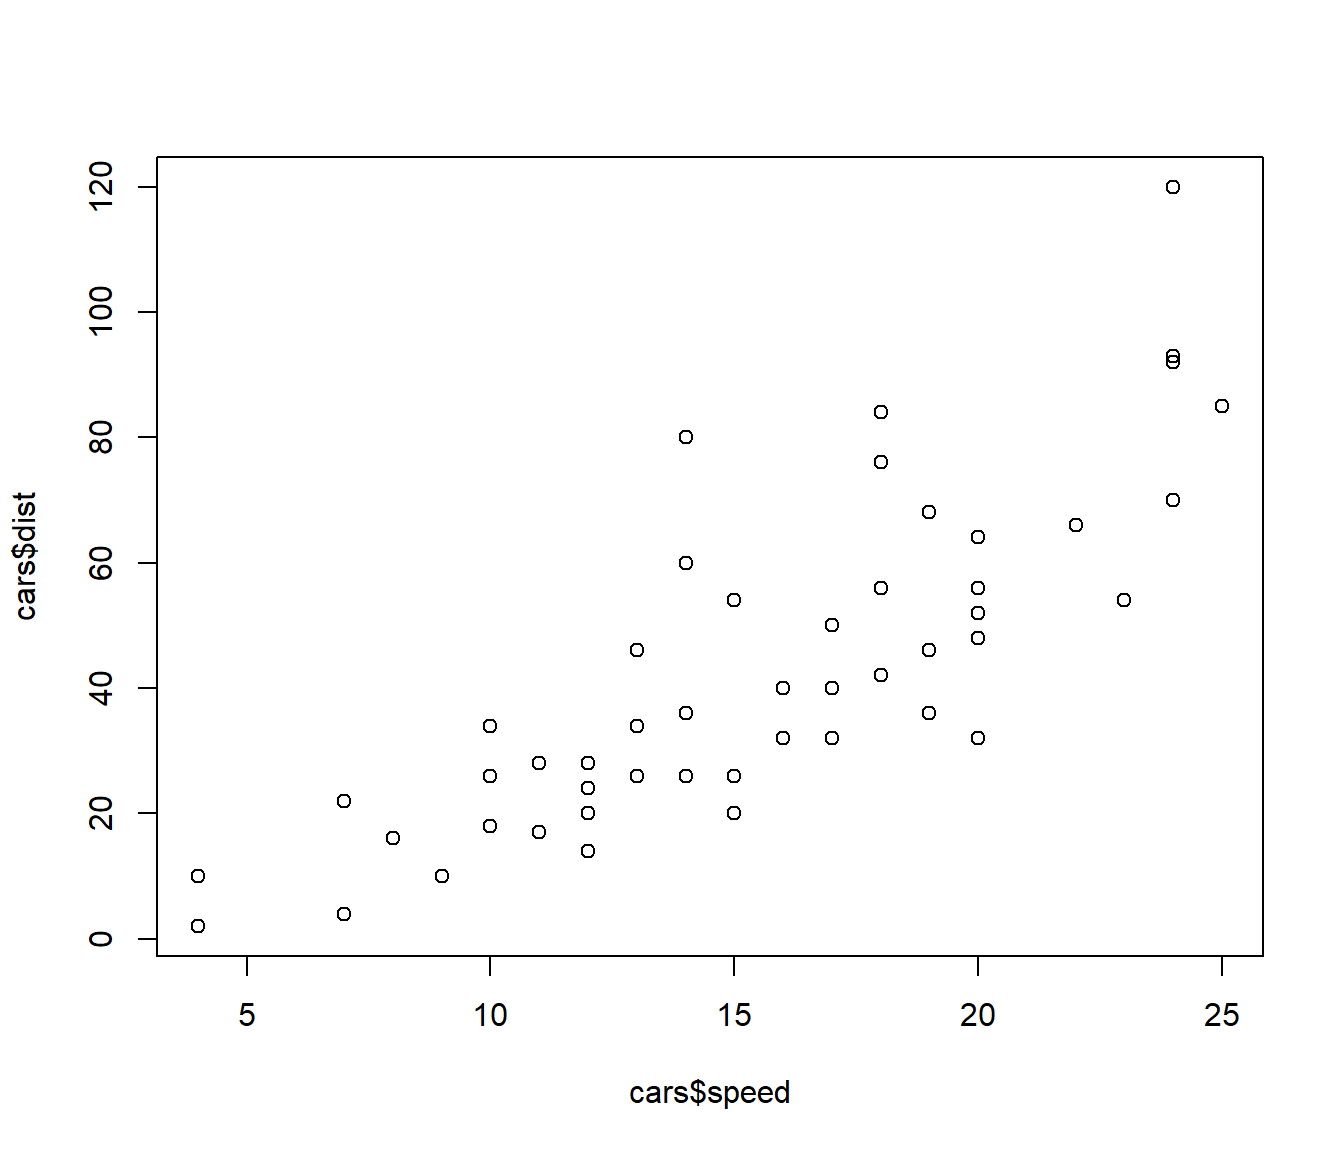
\includegraphics[width=0.7\linewidth]{03-Graficos_files/figure-latex/cars1-1} 

}

\caption{Gráfico de dispersión de distancia frente a velocidad}\label{fig:cars1}
\end{figure}

{[}Figura \ref{fig:cars1}{]}

El comando \texttt{plot} incluye por defecto una elección automáticas de
títulos, ejes, escalas, etiquetas, etc., que pueden ser modificados
añadiendo parámetros gráficos al comando:

\begin{longtable}[]{@{}ll@{}}
\toprule
Parámetro & Descripción\tabularnewline
\midrule
\endhead
\texttt{type} & tipo de gráfico:\tabularnewline
\t & \texttt{p}: puntos, \texttt{l}: líneas, \texttt{b}: puntos y
líneas, \texttt{n}: gráfico en blanco, \ldots{}\tabularnewline
\texttt{xlim}, \texttt{ylim} & límites de los ejes (e.g.
\texttt{xlim=c(1,\ 10)} o \texttt{xlim=range(x)})\tabularnewline
\texttt{xlab}, \texttt{ylab} & títulos de los ejes\tabularnewline
\texttt{main,\ sub} & título principal y subtítulo\tabularnewline
\texttt{col} & color de los símbolos (véase
\texttt{colors()})\tabularnewline
\t & véase \texttt{col.axis}, \texttt{col.lab}, \texttt{col.main},
\texttt{col.sub}\tabularnewline
\texttt{lty} & tipo de línea\tabularnewline
\texttt{lwd} & anchura de línea\tabularnewline
\texttt{pch} & tipo de símbolo\tabularnewline
\texttt{cex} & tamaño de los símbolos\tabularnewline
\texttt{bg} & color de relleno (para
\texttt{pch\ =\ 21:25})\tabularnewline
\bottomrule
\end{longtable}

Para obtener ayuda sobre estos parámetros ejecutar \texttt{help(par)}.

Veamos algún ejemplo:

\begin{Shaded}
\begin{Highlighting}[]
\KeywordTok{plot}\NormalTok{(cars, }\DataTypeTok{xlab =} \StringTok{"velocidad"}\NormalTok{, }\DataTypeTok{ylab =} \StringTok{"distancia"}\NormalTok{, }\DataTypeTok{main =} \StringTok{"Título"}\NormalTok{)}
\end{Highlighting}
\end{Shaded}

\begin{figure}[!htb]

{\centering 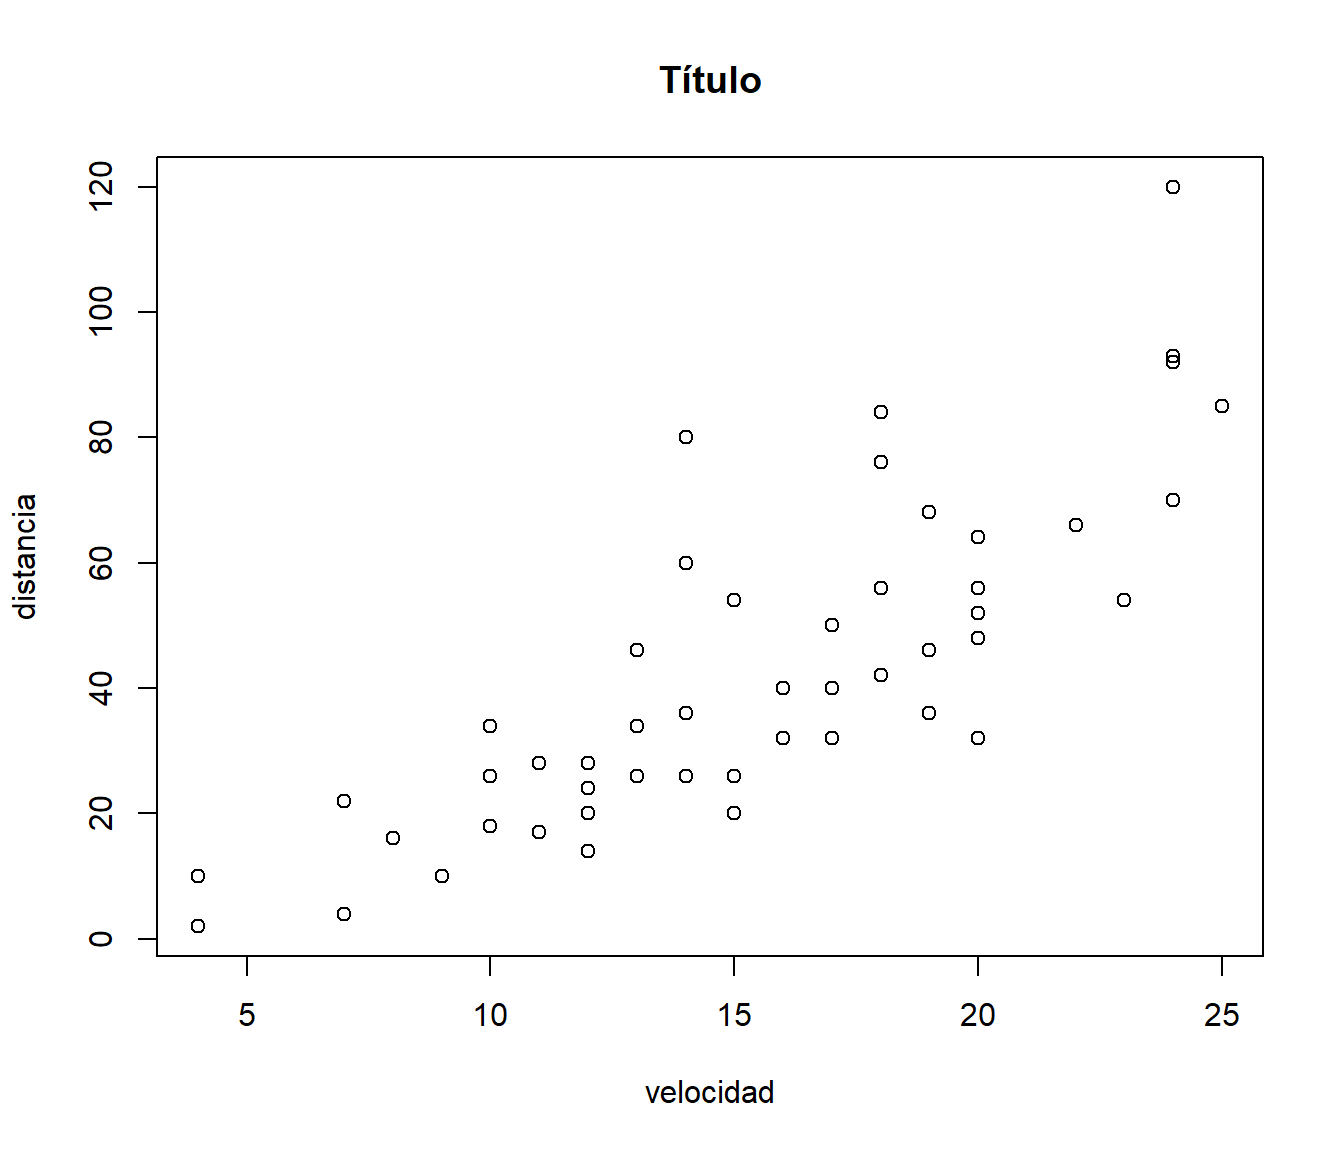
\includegraphics[width=0.7\linewidth]{03-Graficos_files/figure-latex/cars2-1} 

}

\caption{Gráfico de dispersión de distancia frente a velocidad, especificando título y etiquetas de los ejes}\label{fig:cars2}
\end{figure}

{[}Figura \ref{fig:cars2}{]}

\begin{Shaded}
\begin{Highlighting}[]
\KeywordTok{plot}\NormalTok{(cars, }\DataTypeTok{pch =} \DecValTok{16}\NormalTok{, }\DataTypeTok{col =} \StringTok{'blue'}\NormalTok{, }\DataTypeTok{main =} \StringTok{'pch=16'}\NormalTok{)}
\end{Highlighting}
\end{Shaded}

\begin{figure}[!htb]

{\centering 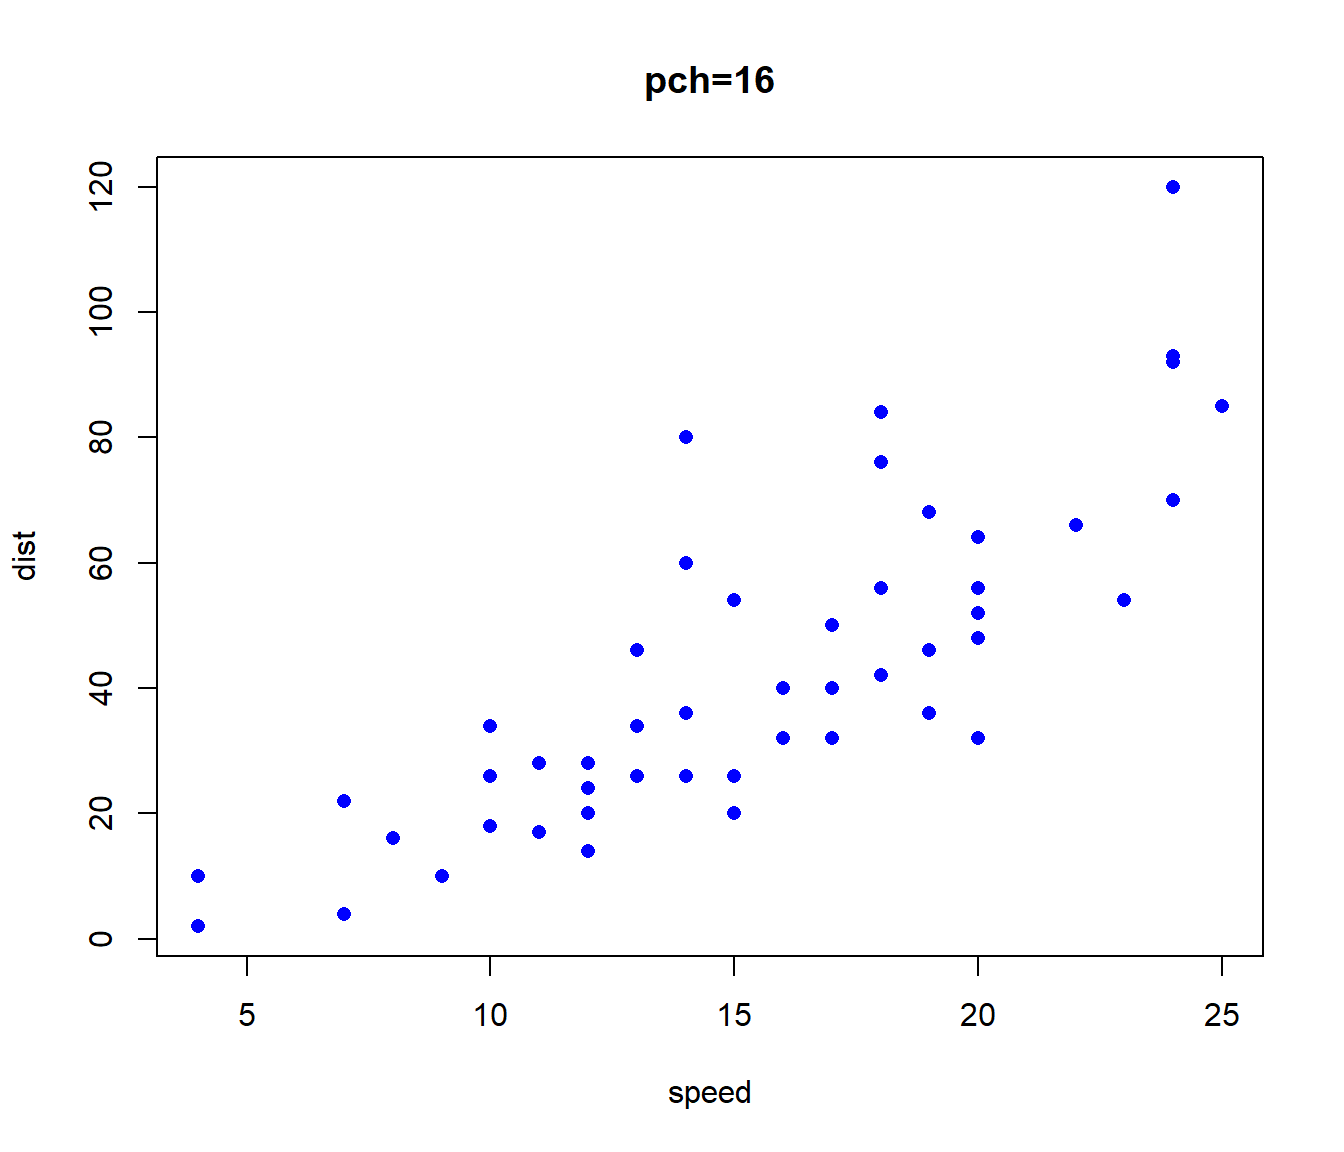
\includegraphics[width=0.7\linewidth]{03-Graficos_files/figure-latex/cars3-1} 

}

\caption{Gráfico de dispersión de distancia frente a velocidad, cambiando el color y el tipo de símbolo}\label{fig:cars3}
\end{figure}

{[}Figura \ref{fig:cars3}{]}

\section{Funciones gráficas de bajo
nivel}\label{funciones-graficas-de-bajo-nivel}

Las principales funciones gráficas de bajo nivel son:

\begin{longtable}[]{@{}ll@{}}
\toprule
Función & Descripción\tabularnewline
\midrule
\endhead
\texttt{points} y \texttt{lines} & agregan puntos y
líneas\tabularnewline
\texttt{text} & agrega un texto\tabularnewline
\texttt{mtext} & agrega texto en los márgenes\tabularnewline
\texttt{segments} & dibuja línea desde el punto inicial al
final\tabularnewline
\texttt{abline} & dibuja líneas\tabularnewline
\texttt{rect} & dibuja rectángulos\tabularnewline
\texttt{polygon} & dibuja polígonos\tabularnewline
\texttt{legend} & agrega una leyenda\tabularnewline
\texttt{axis} & agrega ejes\tabularnewline
\texttt{locator} & devuelve coordenadas de puntos\tabularnewline
\texttt{identify} & similar a \texttt{locator}\tabularnewline
\bottomrule
\end{longtable}

\section{Ejemplos}\label{ejemplos-1}

\begin{Shaded}
\begin{Highlighting}[]
\KeywordTok{plot}\NormalTok{(cars)}
\KeywordTok{abline}\NormalTok{(}\DataTypeTok{h =} \KeywordTok{c}\NormalTok{(}\DecValTok{20}\NormalTok{, }\DecValTok{40}\NormalTok{), }\DataTypeTok{lty =} \DecValTok{2}\NormalTok{) }\CommentTok{# líneas verticales discontinuas (lty=2)}
\CommentTok{# selecciona puntos y los dibuja en azul sólido}
\KeywordTok{points}\NormalTok{(}\KeywordTok{subset}\NormalTok{(cars, dist }\OperatorTok{>}\StringTok{ }\DecValTok{20} \OperatorTok{&}\StringTok{ }\NormalTok{dist }\OperatorTok{<}\StringTok{ }\DecValTok{40}\NormalTok{), }\DataTypeTok{pch =} \DecValTok{16}\NormalTok{, }\DataTypeTok{col =} \StringTok{'blue'}\NormalTok{) }
\end{Highlighting}
\end{Shaded}

\begin{center}\includegraphics[width=0.7\linewidth]{03-Graficos_files/figure-latex/unnamed-chunk-2-1} \end{center}

\begin{Shaded}
\begin{Highlighting}[]
\NormalTok{x <-}\StringTok{ }\KeywordTok{seq}\NormalTok{(}\DecValTok{0}\NormalTok{, }\DecValTok{2} \OperatorTok{*}\StringTok{ }\NormalTok{pi, }\DataTypeTok{length =} \DecValTok{100}\NormalTok{)}
\NormalTok{y1 <-}\StringTok{ }\KeywordTok{cos}\NormalTok{(x)}
\NormalTok{y2 <-}\StringTok{ }\KeywordTok{sin}\NormalTok{(x)}
\KeywordTok{plot}\NormalTok{( x, y1, }\DataTypeTok{type =} \StringTok{"l"}\NormalTok{, }\DataTypeTok{col =} \DecValTok{2}\NormalTok{, }\DataTypeTok{lwd =} \DecValTok{3}\NormalTok{, }\DataTypeTok{xlab =} \StringTok{"[0,2pi]"}\NormalTok{, }\DataTypeTok{ylab =} \StringTok{""}\NormalTok{, }\DataTypeTok{main =} \StringTok{"Seno y Coseno"}\NormalTok{)}
\KeywordTok{lines}\NormalTok{(x, y2, }\DataTypeTok{col =} \DecValTok{3}\NormalTok{, }\DataTypeTok{lwd =} \DecValTok{3}\NormalTok{, }\DataTypeTok{lty =} \DecValTok{2}\NormalTok{)}
\KeywordTok{points}\NormalTok{(pi, }\DecValTok{0}\NormalTok{, }\DataTypeTok{pch =} \DecValTok{17}\NormalTok{, }\DataTypeTok{col =} \DecValTok{4}\NormalTok{)}
\KeywordTok{legend}\NormalTok{(}\DecValTok{0}\NormalTok{, }\OperatorTok{-}\FloatTok{0.5}\NormalTok{, }\KeywordTok{c}\NormalTok{(}\StringTok{"Coseno"}\NormalTok{, }\StringTok{"Seno"}\NormalTok{), }\DataTypeTok{col =} \DecValTok{2}\OperatorTok{:}\DecValTok{3}\NormalTok{, }\DataTypeTok{lty =} \DecValTok{1}\OperatorTok{:}\DecValTok{2}\NormalTok{, }\DataTypeTok{lwd =} \DecValTok{3}\NormalTok{)}

\KeywordTok{abline}\NormalTok{(}\DataTypeTok{v =}\NormalTok{ pi, }\DataTypeTok{lty =} \DecValTok{3}\NormalTok{)}
\KeywordTok{abline}\NormalTok{(}\DataTypeTok{h =} \DecValTok{0}\NormalTok{, }\DataTypeTok{lty =} \DecValTok{3}\NormalTok{)}
\KeywordTok{text}\NormalTok{(pi, }\DecValTok{0}\NormalTok{, }\StringTok{"(pi,0)"}\NormalTok{, }\DataTypeTok{adj =} \KeywordTok{c}\NormalTok{(}\DecValTok{0}\NormalTok{, }\DecValTok{0}\NormalTok{))}
\end{Highlighting}
\end{Shaded}

\begin{center}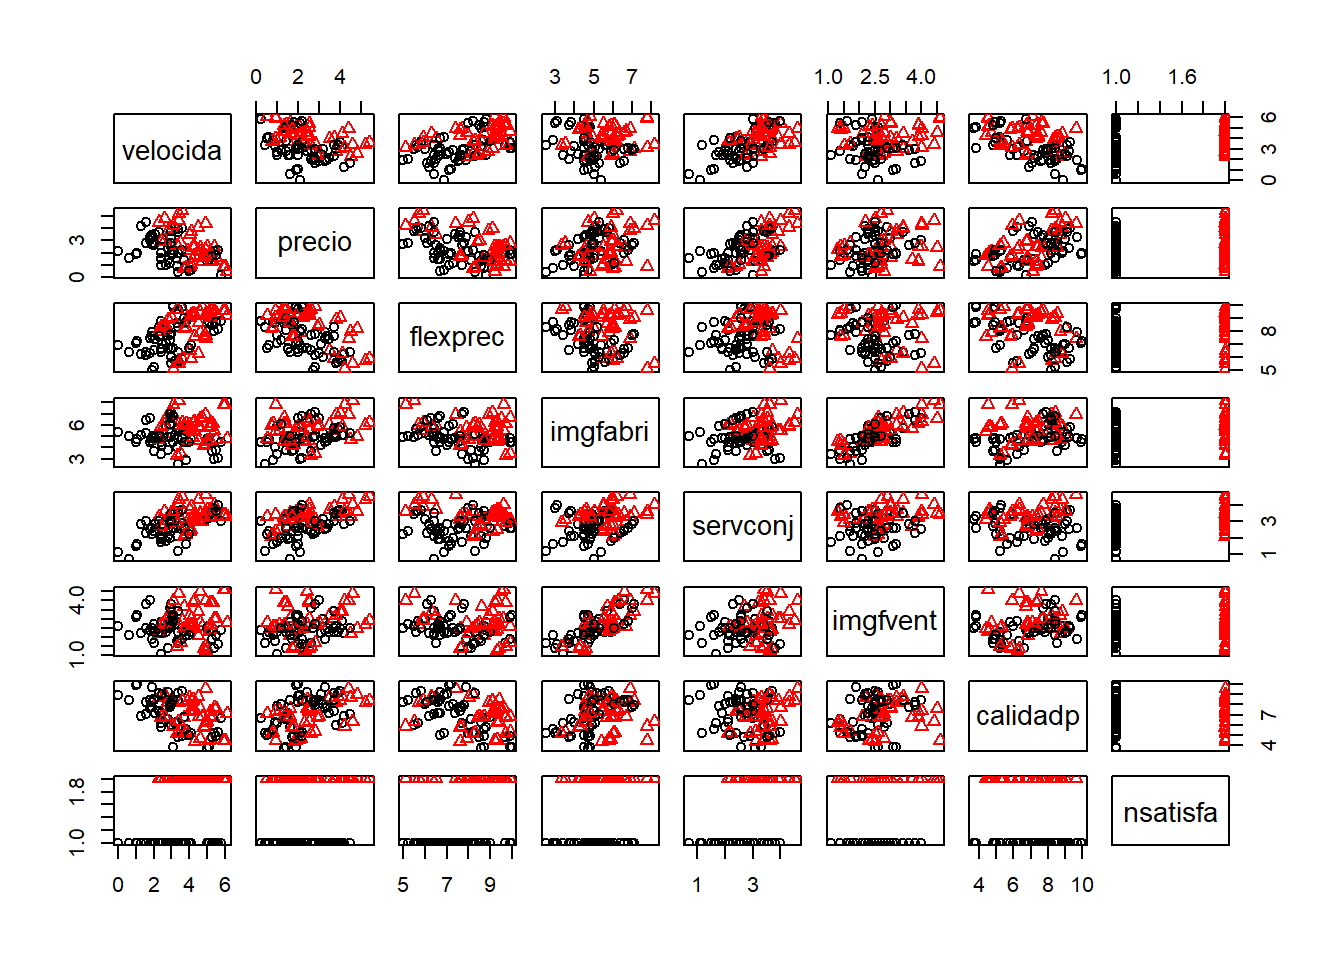
\includegraphics[width=0.7\linewidth]{03-Graficos_files/figure-latex/unnamed-chunk-3-1} \end{center}

Alternativamente se podría usar \texttt{curve()}:

\begin{Shaded}
\begin{Highlighting}[]
\KeywordTok{curve}\NormalTok{(cos, }\DecValTok{0}\NormalTok{, }\DecValTok{2}\OperatorTok{*}\NormalTok{pi, }\DataTypeTok{col =} \DecValTok{2}\NormalTok{, }\DataTypeTok{lwd =} \DecValTok{3}\NormalTok{, }
      \DataTypeTok{xlab =} \StringTok{"[0,2pi]"}\NormalTok{, }\DataTypeTok{ylab =} \StringTok{""}\NormalTok{, }\DataTypeTok{main =} \StringTok{"Seno y Coseno"}\NormalTok{)}
\KeywordTok{curve}\NormalTok{(sin, }\DataTypeTok{col =} \DecValTok{3}\NormalTok{, }\DataTypeTok{lwd =} \DecValTok{3}\NormalTok{, }\DataTypeTok{lty =} \DecValTok{2}\NormalTok{, }\DataTypeTok{add =} \OtherTok{TRUE}\NormalTok{)}
\end{Highlighting}
\end{Shaded}

\begin{center}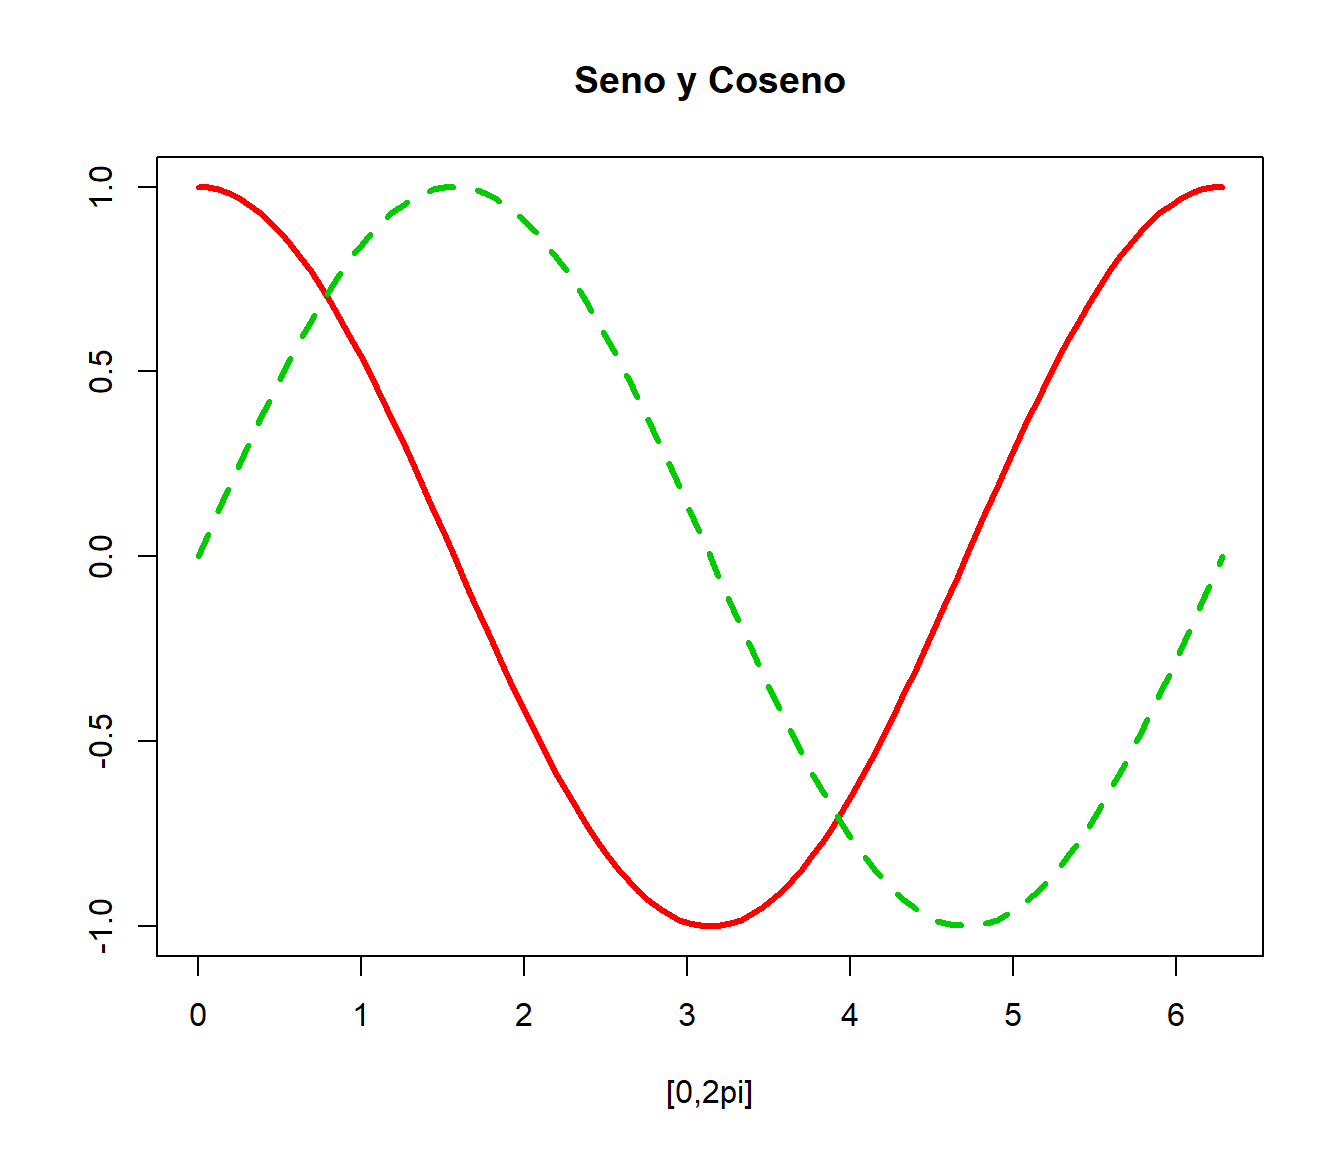
\includegraphics[width=0.7\linewidth]{03-Graficos_files/figure-latex/unnamed-chunk-4-1} \end{center}

\section{Parámetros gráficos}\label{parametros-graficos}

Como ya hemos visto, muchas funciones gráficas permiten establecer
(temporalmente) opciones gráficas mediante estos parámetros. Con la
función \texttt{par()} se pueden obtener y establecer (de forma
permanente) todas las opciones gráficas. Algunas más de estas opciones
son:

\begin{longtable}[]{@{}ll@{}}
\toprule
Parámetro & Descripción\tabularnewline
\midrule
\endhead
\texttt{adj} & justificación del texto\tabularnewline
\texttt{axes} & si es \texttt{FALSE} no dibuja los ejes ni la
caja\tabularnewline
\texttt{bg} & color del fondo\tabularnewline
\texttt{bty} & tipo de caja alrededor del gráfico\tabularnewline
\texttt{font} & estilo del texto\tabularnewline
\ & (1: normal, 2: cursiva, 3:negrita, 4: negrita
cursiva)\tabularnewline
\texttt{las} & orientación de los caracteres en los ejes\tabularnewline
\texttt{mar} & márgenes\tabularnewline
\texttt{mfcol} & divide la pantalla gráfica por columnas\tabularnewline
\texttt{mfrow} & lo mismo que \texttt{mfcol} pero por
filas\tabularnewline
\bottomrule
\end{longtable}

Ejecutar \texttt{help(par)} para obtener la lista completa.

\section{Múltiples gráficos por
ventana}\label{multiples-graficos-por-ventana}

En \texttt{R} se pueden hacer varios gráficos por ventana. Para ello,
antes de ejecutar la función \texttt{plot}, se puede utilizar la
función:

\begin{Shaded}
\begin{Highlighting}[]
\KeywordTok{par}\NormalTok{(}\DataTypeTok{mfrow =} \KeywordTok{c}\NormalTok{(filas, columnas))}
\end{Highlighting}
\end{Shaded}

Los gráficos se irán mostrando en pantalla por filas. En caso de que se
quieran mostrar por columnas en la función anterior se sustituye
\texttt{mfrow} por \texttt{mfcol}.

Por ejemplo, con el siguiente código se obtiene el gráfico de la
siguiente transparencia.

\begin{Shaded}
\begin{Highlighting}[]
\KeywordTok{par}\NormalTok{(}\DataTypeTok{mfrow =} \KeywordTok{c}\NormalTok{(}\DecValTok{2}\NormalTok{, }\DecValTok{3}\NormalTok{))}
\KeywordTok{plot}\NormalTok{(cars, }\DataTypeTok{pch =} \DecValTok{1}\NormalTok{, }\DataTypeTok{main =} \StringTok{"pch = 1"}\NormalTok{)}
\KeywordTok{plot}\NormalTok{(cars, }\DataTypeTok{pch =} \DecValTok{2}\NormalTok{, }\DataTypeTok{main =} \StringTok{"pch = 2"}\NormalTok{)}
\KeywordTok{plot}\NormalTok{(cars, }\DataTypeTok{pch =} \DecValTok{3}\NormalTok{, }\DataTypeTok{main =} \StringTok{"pch = 3"}\NormalTok{)}

\KeywordTok{plot}\NormalTok{(cars, }\DataTypeTok{col =} \StringTok{"red"}\NormalTok{, }\DataTypeTok{main =} \StringTok{"col = red"}\NormalTok{)}
\KeywordTok{plot}\NormalTok{(cars, }\DataTypeTok{col =} \StringTok{"blue"}\NormalTok{, }\DataTypeTok{main =} \StringTok{"col = blue"}\NormalTok{)}
\KeywordTok{plot}\NormalTok{(cars, }\DataTypeTok{col =} \StringTok{"brown"}\NormalTok{, }\DataTypeTok{main =} \StringTok{"col = brown"}\NormalTok{)}
\end{Highlighting}
\end{Shaded}

\begin{center}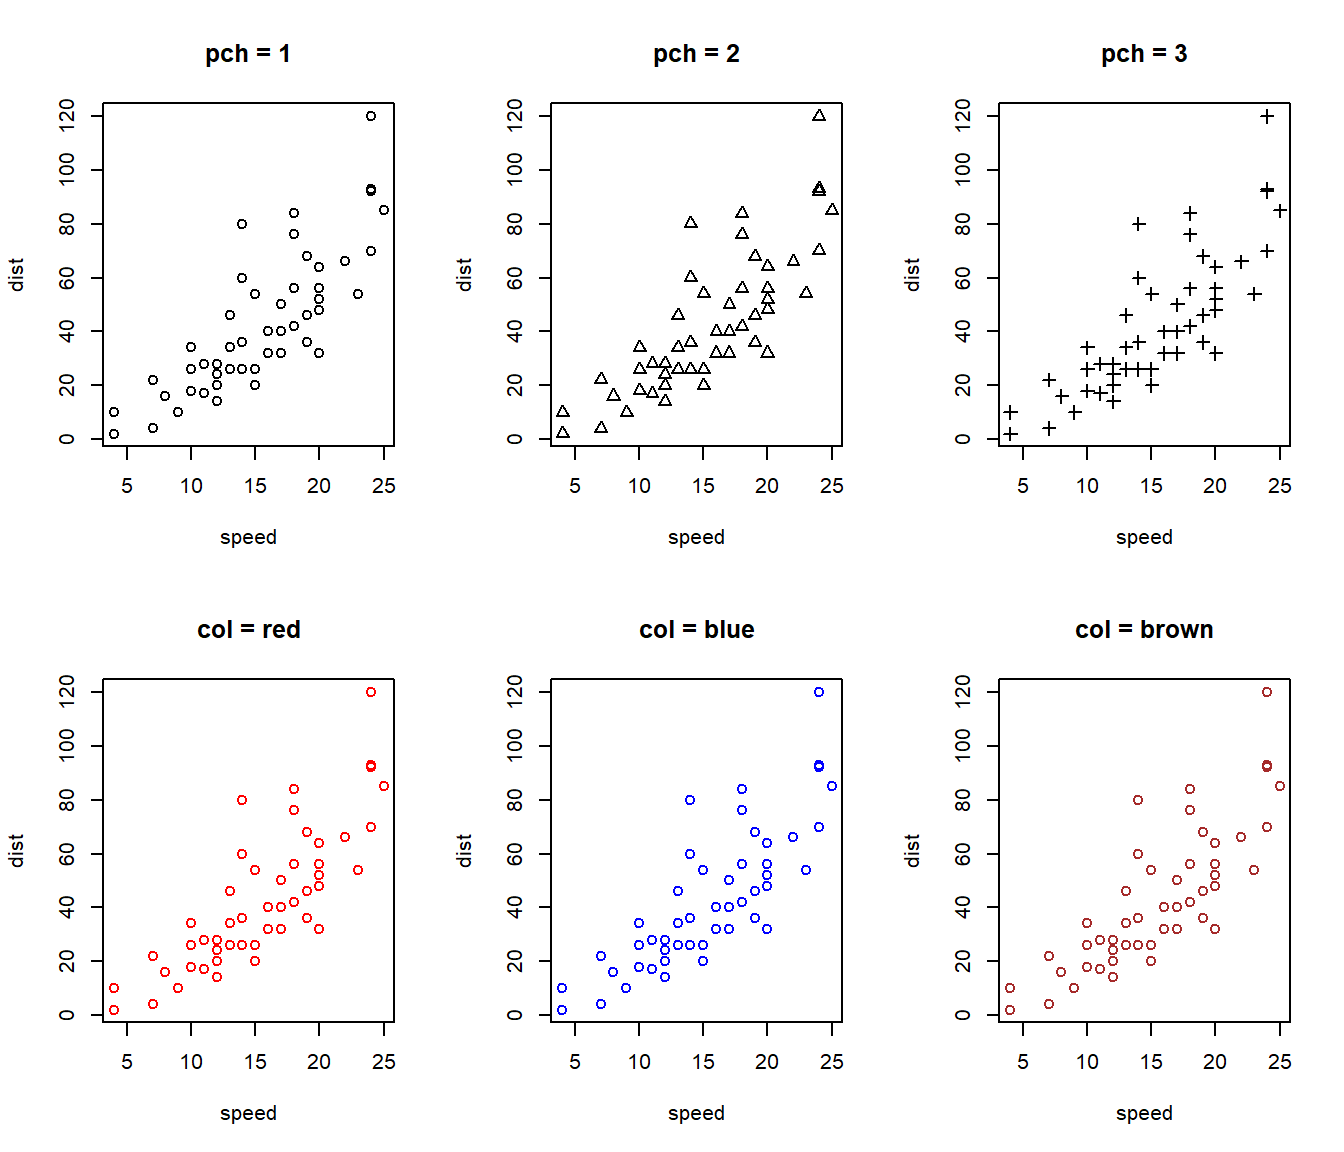
\includegraphics[width=0.7\linewidth]{03-Graficos_files/figure-latex/unnamed-chunk-6-1} \end{center}

Para estructuras gráficas más complicadas véase \texttt{help(layout)}.

\section{Exportar gráficos}\label{exportar-graficos}

Para guardar gráficos, en Windows, se puede usar el menú
\texttt{Archivo\ -\textgreater{}\ Guardar\ como} de la ventana gráfica
(seleccionando el formato deseado: bitmap, postscript,\ldots{}) y
también mediante código ejecutando \texttt{savePlot(filename,\ type)}.
Alternativamente, se pueden emplear ficheros como dispositivos gráficos.
Por ejemplo, a continuación guardamos un gráfico en el fichero
\emph{car.pdf}:

\begin{Shaded}
\begin{Highlighting}[]
\KeywordTok{pdf}\NormalTok{(}\StringTok{"cars.pdf"}\NormalTok{)   }\CommentTok{# abrimos el dispositivo gráfico}
\KeywordTok{plot}\NormalTok{(cars)}
\KeywordTok{dev.off}\NormalTok{()         }\CommentTok{# cerramos el dispositivo}
\end{Highlighting}
\end{Shaded}

Con el siguiente código guardaremos el gráfico en formato jpeg:

\begin{Shaded}
\begin{Highlighting}[]
\KeywordTok{jgeg}\NormalTok{(}\StringTok{"cars.jpg"}\NormalTok{)  }\CommentTok{# abrimos el dispositivo gráfico}
\KeywordTok{plot}\NormalTok{(cars)}
\KeywordTok{dev.off}\NormalTok{()         }\CommentTok{# cerramos el dispositivo}
\end{Highlighting}
\end{Shaded}

Otros formatos disponibles son \texttt{bmp}, \texttt{png} y
\texttt{tiff}. Para más detalles ejecutar:

\begin{Shaded}
\begin{Highlighting}[]
\KeywordTok{help}\NormalTok{(Devices)}
\end{Highlighting}
\end{Shaded}

\section{Otras librerías gráficas}\label{otras-librerias-graficas}

Además de los gráficos estándar, en \texttt{R} están disponibles muchas
librerías gráficas adicionales:

\begin{itemize}
\item
  Gráficos Lattice (Trellis)

  \begin{itemize}
  \item
    Especialmente adecuados para gráficas condicionales múltiples.
  \item
    No se pueden combinar con las funciones estándar.
  \item
    Generalmente el argumento principal es una formula:

    \begin{itemize}
    \item
      \texttt{y\ \textasciitilde{}\ x\ \textbar{}\ a} gráficas de
      \texttt{y} sobre \texttt{x} condicionadas por \texttt{a}
    \item
      \texttt{y\ \textasciitilde{}\ x\ \textbar{}\ a*b} gráficas
      condicionadas por \texttt{a} y \texttt{b}
    \end{itemize}
  \item
    Devuelven un objeto con el que se puede interactuar.
  \end{itemize}
\item
  Más librerías gráficas:

  \begin{itemize}
  \item
    \href{http://had.co.nz/ggplot2}{ggplot2}
  \item
    \href{http://rgl.neoscientists.org}{rgl}
  \item
    \href{http://www.ggobi.org/rggobi}{rggobi}
  \end{itemize}
\end{itemize}

Para más detalles ver
\href{http://cran.r-project.org/web/views/Graphics.html}{CRAN Task View:
Graphics}

\subsection{Ejemplos}\label{ejemplos-2}

\begin{Shaded}
\begin{Highlighting}[]
\KeywordTok{load}\NormalTok{(}\StringTok{"datos/empleados.RData"}\NormalTok{)}
\KeywordTok{library}\NormalTok{(lattice)}
\KeywordTok{xyplot}\NormalTok{(}\KeywordTok{log}\NormalTok{(salario) }\OperatorTok{~}\StringTok{ }\KeywordTok{log}\NormalTok{(salini) }\OperatorTok{|}\StringTok{ }\NormalTok{sexoraza, }\DataTypeTok{data =}\NormalTok{ empleados)}
\end{Highlighting}
\end{Shaded}

\begin{center}\includegraphics[width=0.7\linewidth]{03-Graficos_files/figure-latex/unnamed-chunk-10-1} \end{center}

\begin{Shaded}
\begin{Highlighting}[]
\CommentTok{# Equivalente a xyplot(log(salario) ~ log(salini) | sexo*minoria, data = empleados)}
\end{Highlighting}
\end{Shaded}

\begin{Shaded}
\begin{Highlighting}[]
\KeywordTok{library}\NormalTok{(ggplot2)}
\KeywordTok{ggplot}\NormalTok{(empleados, }\KeywordTok{aes}\NormalTok{(}\KeywordTok{log}\NormalTok{(salini), }\KeywordTok{log}\NormalTok{(salario), }\DataTypeTok{col =}\NormalTok{ sexo)) }\OperatorTok{+}
\StringTok{  }\KeywordTok{geom_point}\NormalTok{() }\OperatorTok{+}
\StringTok{  }\KeywordTok{geom_smooth}\NormalTok{(}\DataTypeTok{method =} \StringTok{"lm"}\NormalTok{, }\DataTypeTok{se =} \OtherTok{FALSE}\NormalTok{)}
\end{Highlighting}
\end{Shaded}

\begin{center}\includegraphics[width=0.7\linewidth]{03-Graficos_files/figure-latex/unnamed-chunk-11-1} \end{center}

\begin{Shaded}
\begin{Highlighting}[]
\KeywordTok{ggplot}\NormalTok{(empleados, }\KeywordTok{aes}\NormalTok{(salario, }\DataTypeTok{fill =}\NormalTok{ sexo)) }\OperatorTok{+}
\StringTok{  }\KeywordTok{geom_density}\NormalTok{(}\DataTypeTok{alpha=}\NormalTok{.}\DecValTok{5}\NormalTok{)}
\end{Highlighting}
\end{Shaded}

\begin{center}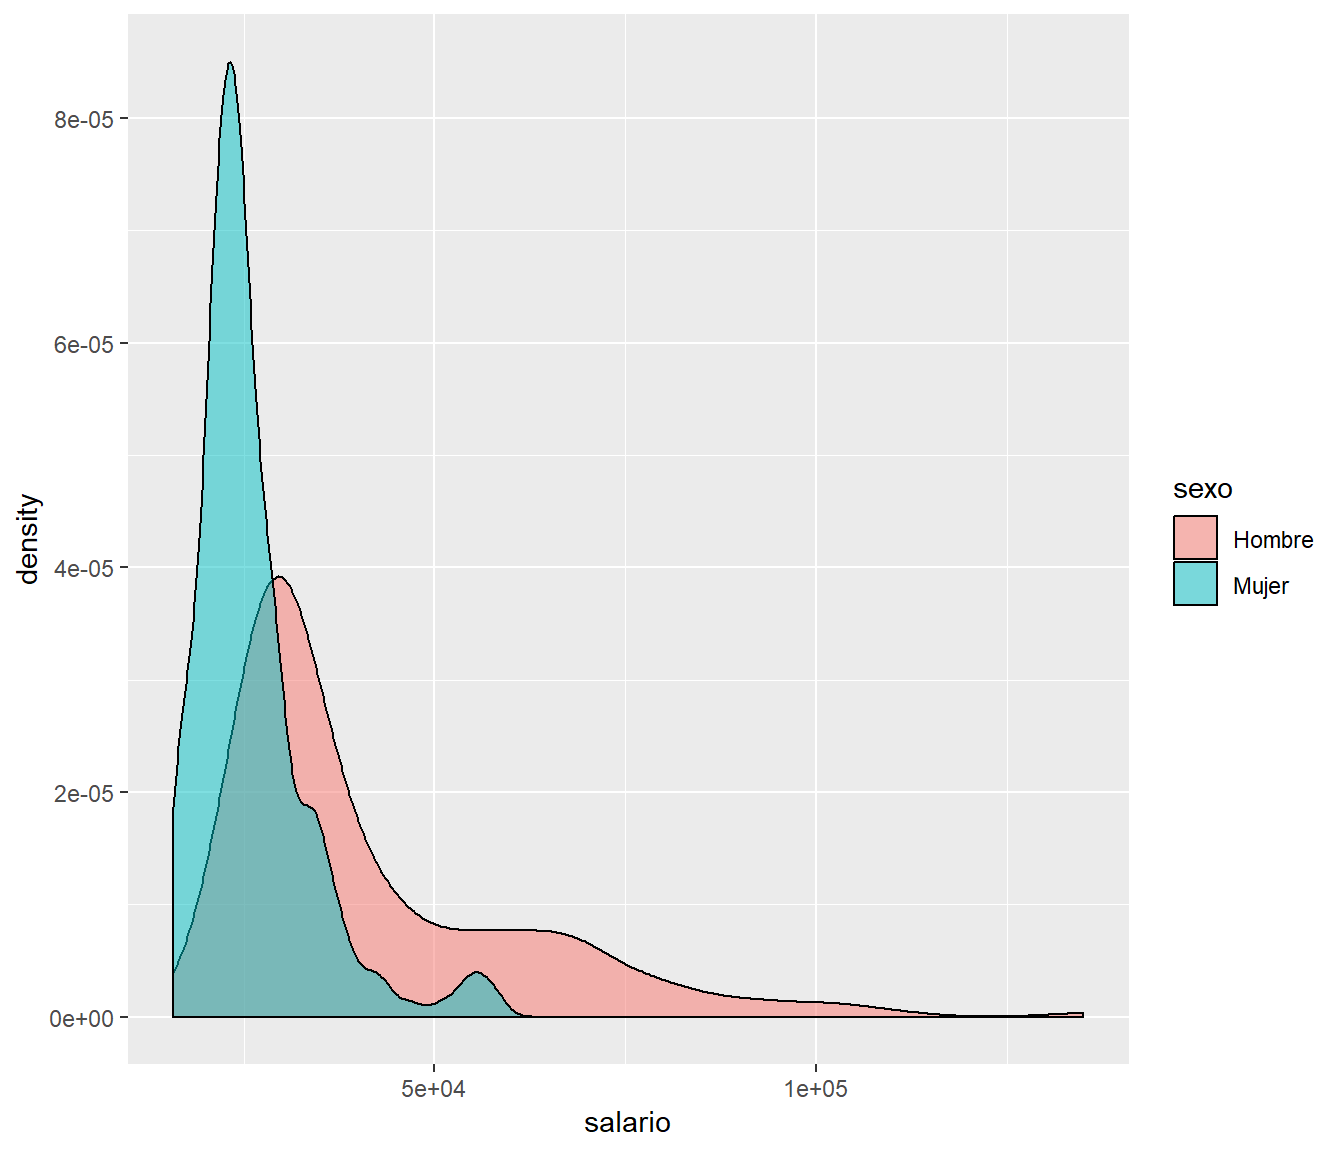
\includegraphics[width=0.7\linewidth]{03-Graficos_files/figure-latex/unnamed-chunk-11-2} \end{center}

\chapter{Manipulación de datos}\label{manipulacion-de-datos}

\section{Lectura, importación y exportación de
datos}\label{lectura-importacion-y-exportacion-de-datos}

La mayoría de los estudios estadísticos requieren disponer de un
conjunto de datos. Además de la introducción directa, \texttt{R} es
capaz de importar datos externos en múltiples formatos:

\begin{itemize}
\item
  bases de datos disponibles en librerías de \texttt{R}
\item
  archivos de texto en formato ASCII
\item
  archivos en otros formatos: Excel, SPSS, \ldots{}
\item
  bases de datos relacionales: MySQL, Oracle, \ldots{}
\item
  formatos web: HTML, XML, JSON, \ldots{}
\item
  \ldots{}.
\end{itemize}

\subsection{Introducción directa}\label{introduccion-directa}

Si los datos son pocos, se pueden teclear directamente en un vector o en
un data.frame. Por ejemplo:

\begin{Shaded}
\begin{Highlighting}[]
\NormalTok{producto <-}\StringTok{ }\KeywordTok{c}\NormalTok{(}\StringTok{"A"}\NormalTok{, }\StringTok{"B"}\NormalTok{, }\StringTok{"C"}\NormalTok{)}
\NormalTok{precio <-}\StringTok{ }\KeywordTok{c}\NormalTok{(}\DecValTok{1200}\NormalTok{, }\DecValTok{560}\NormalTok{, }\DecValTok{740}\NormalTok{)}
\NormalTok{datos <-}\StringTok{ }\KeywordTok{data.frame}\NormalTok{(producto, precio)}
\NormalTok{datos}
\end{Highlighting}
\end{Shaded}

\begin{verbatim}
##   producto precio
## 1        A   1200
## 2        B    560
## 3        C    740
\end{verbatim}

En ocasiones, tanto para matrices como para data.frames, será de
utilidad la función \texttt{edit}. Por ejemplo, una sentencia como:

\begin{Shaded}
\begin{Highlighting}[]
\NormalTok{datos2 <-}\StringTok{ }\KeywordTok{edit}\NormalTok{(datos)}
\end{Highlighting}
\end{Shaded}

abre una hoja de cálculo ``muy básica'' con la que podremos editar los
elementos del data.frame, cambiar sus dimensiones añadiendo filas y/o
columnas, \ldots{}

\textbf{Nota}: Hay que destacar que \texttt{datos} tiene que existir
antes de emplear la función \texttt{edit}. Para modificar directamente
el objeto puede ser más cómodo emplear la función \texttt{fix()}.

\subsection{Lectura desde paquetes}\label{lectura-desde-paquetes}

El programa \texttt{R} dispone de múltiples conjuntos de datos. Al
teclear:

\begin{Shaded}
\begin{Highlighting}[]
\KeywordTok{data}\NormalTok{()}
\end{Highlighting}
\end{Shaded}

se obtiene un listado de las bases de datos disponibles.

\begin{verbatim}
Data sets in package "datasets":

AirPassengers           Monthly Airline Passenger Numbers 1949-1960
BJsales                 Sales Data with Leading Indicator
BJsales.lead (BJsales)
                        Sales Data with Leading Indicator
BOD                     Biochemical Oxygen Demand
CO2                     Carbon Dioxide Uptake in Grass Plants
ChickWeight             Weight versus age of chicks on different diets

.....
\end{verbatim}

Para cargar una base de datos concreta se utiliza el comando
\texttt{data(nombre)} (aunque en algunos casos se cargan
automáticamente). Por ejemplo, la base de datos llamada \texttt{cars} se
carga con:

\begin{Shaded}
\begin{Highlighting}[]
\KeywordTok{data}\NormalTok{(cars)}
\end{Highlighting}
\end{Shaded}

Una vez cargado el objeto \texttt{cars} (\texttt{R} lo carga como un
data.frame), se podrán utilizar las correspondientes sentencias para
realizar resúmenes numéricos y gráficos.

\begin{Shaded}
\begin{Highlighting}[]
\KeywordTok{head}\NormalTok{(cars)  }\CommentTok{# Primeros valores}
\end{Highlighting}
\end{Shaded}

\begin{verbatim}
##   speed dist
## 1     4    2
## 2     4   10
## 3     7    4
## 4     7   22
## 5     8   16
## 6     9   10
\end{verbatim}

\begin{Shaded}
\begin{Highlighting}[]
\KeywordTok{help}\NormalTok{(cars)  }\CommentTok{# Obtención de ayuda}
\end{Highlighting}
\end{Shaded}

\begin{verbatim}
...

Speed and Stopping Distances of Cars

Description:
     The data give the speed of cars and the distances taken to stop.
     Note that the data were recorded in the 1920s.

...  

Format:
     A data frame with 50 observations on 2 variables.
       [,1]  speed  numeric  Speed (mph)            
       [,2]  dist   numeric  Stopping distance (ft) 
      
Source:
     Ezekiel, M. (1930) _Methods of Correlation Analysis_.  Wiley.
     
...  
\end{verbatim}

\begin{Shaded}
\begin{Highlighting}[]
\KeywordTok{names}\NormalTok{(cars)      }\CommentTok{# Nombres}
\end{Highlighting}
\end{Shaded}

\begin{verbatim}
## [1] "speed" "dist"
\end{verbatim}

\begin{Shaded}
\begin{Highlighting}[]
\NormalTok{cars}\OperatorTok{$}\NormalTok{speed[}\DecValTok{1}\OperatorTok{:}\DecValTok{10}\NormalTok{] }\CommentTok{# Primeros 10 valores de velocidad}
\end{Highlighting}
\end{Shaded}

\begin{verbatim}
##  [1]  4  4  7  7  8  9 10 10 10 11
\end{verbatim}

\begin{Shaded}
\begin{Highlighting}[]
\NormalTok{cars}\OperatorTok{$}\NormalTok{dist[}\DecValTok{1}\OperatorTok{:}\DecValTok{10}\NormalTok{] }\CommentTok{# Primeros 10 valores de distancia}
\end{Highlighting}
\end{Shaded}

\begin{verbatim}
##  [1]  2 10  4 22 16 10 18 26 34 17
\end{verbatim}

\begin{Shaded}
\begin{Highlighting}[]
\KeywordTok{names}\NormalTok{(cars) <-}\StringTok{ }\KeywordTok{c}\NormalTok{(}\StringTok{"velocidad"}\NormalTok{, }\StringTok{"distancia"}\NormalTok{)  }\CommentTok{# Nombres en español}
\KeywordTok{head}\NormalTok{(cars)}
\end{Highlighting}
\end{Shaded}

\begin{verbatim}
##   velocidad distancia
## 1         4         2
## 2         4        10
## 3         7         4
## 4         7        22
## 5         8        16
## 6         9        10
\end{verbatim}

\begin{Shaded}
\begin{Highlighting}[]
\KeywordTok{summary}\NormalTok{(cars)   }\CommentTok{# Resumen estadístico}
\end{Highlighting}
\end{Shaded}

\begin{verbatim}
##    velocidad      distancia     
##  Min.   : 4.0   Min.   :  2.00  
##  1st Qu.:12.0   1st Qu.: 26.00  
##  Median :15.0   Median : 36.00  
##  Mean   :15.4   Mean   : 42.98  
##  3rd Qu.:19.0   3rd Qu.: 56.00  
##  Max.   :25.0   Max.   :120.00
\end{verbatim}

\begin{Shaded}
\begin{Highlighting}[]
\KeywordTok{plot}\NormalTok{(cars)             }\CommentTok{# Gráfico de dispersión de los datos}
\KeywordTok{hist}\NormalTok{(cars}\OperatorTok{$}\NormalTok{velocidad)    }\CommentTok{# Histograma de velocidad}
\KeywordTok{boxplot}\NormalTok{(cars}\OperatorTok{$}\NormalTok{distancia) }\CommentTok{# Boxplot de distancia}
\end{Highlighting}
\end{Shaded}

\subsection{Lectura de archivos de
texto}\label{lectura-de-archivos-de-texto}

En \texttt{R} para leer archivos de texto se suele utilizar la función
\texttt{read.table()}.

Supóngase, por ejemplo, que en el directorio actual está el fichero
\emph{empleados.txt}. La lectura de este fichero vendría dada por el
código:

\begin{Shaded}
\begin{Highlighting}[]
\NormalTok{datos <-}\StringTok{ }\KeywordTok{read.table}\NormalTok{(}\DataTypeTok{file =} \StringTok{"datos/empleados.txt"}\NormalTok{, }\DataTypeTok{header =} \OtherTok{TRUE}\NormalTok{)}
\KeywordTok{head}\NormalTok{(datos)}
\end{Highlighting}
\end{Shaded}

\begin{verbatim}
##   id   sexo   fechnac educ         catlab salario salini tiempemp expprev
## 1  1 Hombre  2/3/1952   15      Directivo   57000  27000       98     144
## 2  2 Hombre 5/23/1958   16 Administrativo   40200  18750       98      36
## 3  3  Mujer 7/26/1929   12 Administrativo   21450  12000       98     381
## 4  4  Mujer 4/15/1947    8 Administrativo   21900  13200       98     190
## 5  5 Hombre  2/9/1955   15 Administrativo   45000  21000       98     138
## 6  6 Hombre 8/22/1958   15 Administrativo   32100  13500       98      67
##   minoria
## 1      No
## 2      No
## 3      No
## 4      No
## 5      No
## 6      No
\end{verbatim}

Si el fichero estuviese en el directorio \emph{c:\textbackslash{}datos}
bastaría con especificar \texttt{file\ =\ "c:/datos/empleados.txt"}.
Nótese también que para la lectura del fichero anterior se ha
establecido el argumento \texttt{header=TRUE} para indicar que la
primera línea del fichero contiene los nombres de las variables.

Los argumentos utilizados habitualmente para esta función son:

\begin{itemize}
\item
  \texttt{header}: indica si el fichero tiene cabecera
  (\texttt{header=TRUE}) o no (\texttt{header=FALSE}). Por defecto toma
  el valor \texttt{header=FALSE}.
\item
  \texttt{sep}: carácter separador de columnas que por defecto es un
  espacio en blanco (\texttt{sep=""}). Otras opciones serían:
  \texttt{sep=","} si el separador es un ``;'', \texttt{sep="*"} si el
  separador es un ``*'', etc.
\item
  \texttt{dec}: carácter utilizado en el fichero para los números
  decimales. Por defecto se establece \texttt{dec\ =\ "."}. Si los
  decimales vienen dados por ``,'' se utiliza \texttt{dec\ =\ ","}
\end{itemize}

Resumiendo, los (principales) argumentos por defecto de la función
\texttt{read.table} son los que se muestran en la siguiente línea:

\begin{Shaded}
\begin{Highlighting}[]
\KeywordTok{read.table}\NormalTok{(file, }\DataTypeTok{header =} \OtherTok{FALSE}\NormalTok{, }\DataTypeTok{sep =} \StringTok{""}\NormalTok{, }\DataTypeTok{dec =} \StringTok{"."}\NormalTok{)  }
\end{Highlighting}
\end{Shaded}

Para más detalles sobre esta función véase \texttt{help(read.table)}.

Estan disponibles otras funciones con valores por defecto de los
parámetros adecuados para otras situaciones. Por ejemplo, para ficheros
separados por tabuladores se puede utilizar \texttt{read.delim()} o
\texttt{read.delim2()}:

\begin{Shaded}
\begin{Highlighting}[]
\KeywordTok{read.delim}\NormalTok{(file, }\DataTypeTok{header =} \OtherTok{TRUE}\NormalTok{, }\DataTypeTok{sep =} \StringTok{"}\CharTok{\textbackslash{}t}\StringTok{"}\NormalTok{, }\DataTypeTok{dec =} \StringTok{"."}\NormalTok{)}
\KeywordTok{read.delim2}\NormalTok{(file, }\DataTypeTok{header =} \OtherTok{TRUE}\NormalTok{, }\DataTypeTok{sep =} \StringTok{"}\CharTok{\textbackslash{}t}\StringTok{"}\NormalTok{, }\DataTypeTok{dec =} \StringTok{","}\NormalTok{)}
\end{Highlighting}
\end{Shaded}

\subsection{Importación desde SPSS}\label{importacion-desde-spss}

El programa \texttt{R} permite lectura de ficheros de datos en formato
SPSS (extensión \emph{.sav}) sin necesidad de tener instalado dicho
programa en el ordenador. Para ello se necesita:

\begin{itemize}
\item
  cargar la librería \texttt{foreign}
\item
  utilizar la función \texttt{read.spss}
\end{itemize}

Por ejemplo:

\begin{Shaded}
\begin{Highlighting}[]
\KeywordTok{library}\NormalTok{(foreign)}
\NormalTok{datos <-}\StringTok{ }\KeywordTok{read.spss}\NormalTok{(}\DataTypeTok{file =} \StringTok{"datos/Employee data.sav"}\NormalTok{, }\DataTypeTok{to.data.frame =} \OtherTok{TRUE}\NormalTok{)}
\KeywordTok{head}\NormalTok{(datos)}
\end{Highlighting}
\end{Shaded}

\begin{verbatim}
##   id   sexo     fechnac educ         catlab salario salini tiempemp
## 1  1 Hombre 11654150400   15      Directivo   57000  27000       98
## 2  2 Hombre 11852956800   16 Administrativo   40200  18750       98
## 3  3  Mujer 10943337600   12 Administrativo   21450  12000       98
## 4  4  Mujer 11502518400    8 Administrativo   21900  13200       98
## 5  5 Hombre 11749363200   15 Administrativo   45000  21000       98
## 6  6 Hombre 11860819200   15 Administrativo   32100  13500       98
##   expprev minoria
## 1     144      No
## 2      36      No
## 3     381      No
## 4     190      No
## 5     138      No
## 6      67      No
\end{verbatim}

\textbf{Nota}: Si hay fechas, puede ser recomendable emplear la función
\texttt{spss.get()} del paquete \texttt{Hmisc}.

\subsection{Importación desde Excel}\label{importacion-desde-excel}

Se pueden leer fichero de Excel (con extensión \emph{.xls}) utilizando
por ejemplo funciones de las librerías \texttt{openxlsx},
\texttt{XLConnect} o \texttt{RODBC}. Sin embargo, puede ser recomendable
exportar los datos desde Excel a un archivo de texto separado por
tabuladores (extensión \emph{.csv}).

Por ejemplo, supongamos que queremos leer el fichero \emph{coches.xls}:

\begin{itemize}
\item
  Desde Excel se selecciona el menú
  \texttt{Archivo\ -\textgreater{}\ Guardar\ como\ -\textgreater{}\ Guardar\ como}
  y en \texttt{Tipo} se escoge la opción de archivo CSV. De esta forma
  se guardarán los datos en el archivo \emph{coches.csv}.
\item
  El fichero \emph{coches.csv} es un fichero de texto plano (se puede
  editar con Notepad), con cabecera, las columnas separadas por ``;'', y
  siendo ``,'' el carácter decimal.
\item
  Por lo tanto, la lectura de este fichero se puede hacer con:

\begin{Shaded}
\begin{Highlighting}[]
\NormalTok{datos <-}\StringTok{ }\KeywordTok{read.table}\NormalTok{(}\StringTok{"datos/coches.csv"}\NormalTok{, }\DataTypeTok{header =} \OtherTok{TRUE}\NormalTok{, }\DataTypeTok{sep =} \StringTok{";"}\NormalTok{, }\DataTypeTok{dec =} \StringTok{","}\NormalTok{)}
\end{Highlighting}
\end{Shaded}
\end{itemize}

Otra posibilidad es utilizar la función \texttt{read.csv2}, que es una
adaptación de la función general \texttt{read.table} con la siguiente
configuración.

\begin{Shaded}
\begin{Highlighting}[]
\KeywordTok{read.csv2}\NormalTok{(file, }\DataTypeTok{header =} \OtherTok{TRUE}\NormalTok{, }\DataTypeTok{sep =} \StringTok{";"}\NormalTok{, }\DataTypeTok{dec =} \StringTok{","}\NormalTok{)}
\end{Highlighting}
\end{Shaded}

Por lo tanto, la lectura del fichero \emph{coches.csv} se puede hacer de
modo más directo con

\begin{Shaded}
\begin{Highlighting}[]
\NormalTok{datos <-}\StringTok{ }\KeywordTok{read.csv2}\NormalTok{(}\StringTok{"datos/coches.csv"}\NormalTok{)}
\end{Highlighting}
\end{Shaded}

\subsection{Exportación de datos}\label{exportacion-de-datos}

Es evidente que además de la lectura e importación de datos también será
de gran interés la exportación de datos para que puedan leídos con otros
programas. Para ello, es de gran utilidad la función
\texttt{write.table}. Esta función es similar, pero funcionando en
sentido inverso, a la ya vista \texttt{read.table}.

Veamos un ejemplo:

\begin{Shaded}
\begin{Highlighting}[]
\NormalTok{tipo <-}\StringTok{ }\KeywordTok{c}\NormalTok{(}\StringTok{"A"}\NormalTok{, }\StringTok{"B"}\NormalTok{, }\StringTok{"C"}\NormalTok{)}
\NormalTok{longitud <-}\StringTok{ }\KeywordTok{c}\NormalTok{(}\FloatTok{120.34}\NormalTok{, }\FloatTok{99.45}\NormalTok{, }\FloatTok{115.67}\NormalTok{)}
\NormalTok{datos <-}\StringTok{ }\KeywordTok{data.frame}\NormalTok{(tipo, longitud)}
\NormalTok{datos}
\end{Highlighting}
\end{Shaded}

\begin{verbatim}
##   tipo longitud
## 1    A   120.34
## 2    B    99.45
## 3    C   115.67
\end{verbatim}

Para guardar el data.frame \texttt{datos} en un fichero de texto se
utiliza se puede utilizar

\begin{Shaded}
\begin{Highlighting}[]
\KeywordTok{write.table}\NormalTok{(datos, }\DataTypeTok{file =} \StringTok{"datos.txt"}\NormalTok{)}
\end{Highlighting}
\end{Shaded}

Otra posibilidad es utilizar la función

\begin{Shaded}
\begin{Highlighting}[]
\KeywordTok{write.csv2}\NormalTok{(datos, }\DataTypeTok{file =} \StringTok{"datos.csv"}\NormalTok{)}
\end{Highlighting}
\end{Shaded}

que dará lugar al fichero \emph{datos.csv} importable directamente desde
Excel.

\section{Manipulación de datos}\label{manipulacion-de-datos-1}

Una vez cargada una (o varias) bases de datos hay una series de
operaciones que serán de interés para el tratamiento de datos:

\begin{itemize}
\tightlist
\item
  Operaciones con variables:

  \begin{itemize}
  \tightlist
  \item
    creación
  \item
    recodificación (e.g.~categorización)
  \item
    \ldots{}
  \end{itemize}
\item
  Operaciones con casos:

  \begin{itemize}
  \tightlist
  \item
    ordenación
  \item
    filtrado de datos
  \item
    \ldots{}
  \end{itemize}
\end{itemize}

A continuación se tratan las operaciones más básicas.

\subsection{Operaciones con variables}\label{operaciones-con-variables}

\subsubsection{Creación (y eliminación) de
variables}\label{creacion-y-eliminacion-de-variables}

Consideremos de nuevo la base de datos \texttt{cars} incluida en el
paquete \texttt{datasets}.

\begin{Shaded}
\begin{Highlighting}[]
\KeywordTok{data}\NormalTok{(cars)}
\KeywordTok{head}\NormalTok{(cars)}
\end{Highlighting}
\end{Shaded}

\begin{verbatim}
##   speed dist
## 1     4    2
## 2     4   10
## 3     7    4
## 4     7   22
## 5     8   16
## 6     9   10
\end{verbatim}

Utilizando el comando \texttt{help(cars)} se obtiene que \texttt{cars}
es un data.frame con 50 observaciones y dos variables:

\begin{itemize}
\item
  \texttt{speed}: Velocidad (millas por hora)
\item
  \texttt{dist}: tiempo hasta detenerse (pies)
\end{itemize}

Recordemos que, para acceder a la variable \texttt{speed} se puede hacer
directamente con su nombre o bien utilizando notación ``matricial''.

\begin{Shaded}
\begin{Highlighting}[]
\NormalTok{cars}\OperatorTok{$}\NormalTok{speed}
\end{Highlighting}
\end{Shaded}

\begin{verbatim}
##  [1]  4  4  7  7  8  9 10 10 10 11 11 12 12 12 12 13 13 13 13 14 14 14 14
## [24] 15 15 15 16 16 17 17 17 18 18 18 18 19 19 19 20 20 20 20 20 22 23 24
## [47] 24 24 24 25
\end{verbatim}

\begin{Shaded}
\begin{Highlighting}[]
\NormalTok{cars[, }\DecValTok{1}\NormalTok{]  }\CommentTok{# Equivalente}
\end{Highlighting}
\end{Shaded}

\begin{verbatim}
##  [1]  4  4  7  7  8  9 10 10 10 11 11 12 12 12 12 13 13 13 13 14 14 14 14
## [24] 15 15 15 16 16 17 17 17 18 18 18 18 19 19 19 20 20 20 20 20 22 23 24
## [47] 24 24 24 25
\end{verbatim}

Supongamos ahora que queremos transformar la variable original
\texttt{speed} (millas por hora) en una nueva variable
\texttt{velocidad} (kilómetros por hora) y añadir esta nueva variable al
data.frame \texttt{cars}.

La transformación que permite pasar millas a kilómetros es
kilómetros=millas/0.62137 que en \texttt{R} se hace directamente con:

\begin{Shaded}
\begin{Highlighting}[]
\NormalTok{cars}\OperatorTok{$}\NormalTok{speed}\OperatorTok{/}\FloatTok{0.62137}
\end{Highlighting}
\end{Shaded}

Finalmente, incluimos la nueva variable que llamaremos
\texttt{velocidad} en \texttt{cars}.

\begin{Shaded}
\begin{Highlighting}[]
\NormalTok{cars}\OperatorTok{$}\NormalTok{velocidad <-}\StringTok{ }\NormalTok{cars}\OperatorTok{$}\NormalTok{speed }\OperatorTok{/}\StringTok{ }\FloatTok{0.62137}
\KeywordTok{head}\NormalTok{(cars)}
\end{Highlighting}
\end{Shaded}

\begin{verbatim}
##   speed dist velocidad
## 1     4    2  6.437388
## 2     4   10  6.437388
## 3     7    4 11.265430
## 4     7   22 11.265430
## 5     8   16 12.874777
## 6     9   10 14.484124
\end{verbatim}

También transformaremos la variable \texttt{dist} (en pies) en una nueva
variable \texttt{distancia} (en metros). Ahora la transformación deseada
es \texttt{metros=pies/3.2808}.

\begin{Shaded}
\begin{Highlighting}[]
\NormalTok{cars}\OperatorTok{$}\NormalTok{distancia <-}\StringTok{ }\NormalTok{cars}\OperatorTok{$}\NormalTok{dis }\OperatorTok{/}\StringTok{ }\FloatTok{3.2808}
\KeywordTok{head}\NormalTok{(cars)}
\end{Highlighting}
\end{Shaded}

\begin{verbatim}
##   speed dist velocidad distancia
## 1     4    2  6.437388 0.6096074
## 2     4   10  6.437388 3.0480371
## 3     7    4 11.265430 1.2192148
## 4     7   22 11.265430 6.7056815
## 5     8   16 12.874777 4.8768593
## 6     9   10 14.484124 3.0480371
\end{verbatim}

Ahora, eliminaremos las variables originales \texttt{speed} y
\texttt{dist}, y guardaremos el data.frame resultante con el nombre
\texttt{coches}. En primer lugar, veamos varias formas de acceder a las
variables de interés

\begin{Shaded}
\begin{Highlighting}[]
\NormalTok{cars[, }\KeywordTok{c}\NormalTok{(}\DecValTok{3}\NormalTok{, }\DecValTok{4}\NormalTok{)]}
\NormalTok{cars[, }\KeywordTok{c}\NormalTok{(}\StringTok{"velocidad"}\NormalTok{, }\StringTok{"distancia"}\NormalTok{)]}
\NormalTok{cars[, }\OperatorTok{-}\KeywordTok{c}\NormalTok{(}\DecValTok{1}\NormalTok{, }\DecValTok{2}\NormalTok{)]}
\end{Highlighting}
\end{Shaded}

Utilizando alguna de las opciones anteriores se obtiene el data.frame
deseado.

\begin{Shaded}
\begin{Highlighting}[]
\NormalTok{coches <-}\StringTok{ }\NormalTok{cars[, }\KeywordTok{c}\NormalTok{(}\StringTok{"velocidad"}\NormalTok{, }\StringTok{"distancia"}\NormalTok{)]}
\KeywordTok{head}\NormalTok{(coches)}
\end{Highlighting}
\end{Shaded}

\begin{verbatim}
##   velocidad distancia
## 1  6.437388 0.6096074
## 2  6.437388 3.0480371
## 3 11.265430 1.2192148
## 4 11.265430 6.7056815
## 5 12.874777 4.8768593
## 6 14.484124 3.0480371
\end{verbatim}

Finalmente los datos anteriores podrían ser guardados en un fichero
exportable a Excel con el siguiente comando:

\begin{Shaded}
\begin{Highlighting}[]
\KeywordTok{write.csv2}\NormalTok{(coches, }\DataTypeTok{file =} \StringTok{"coches.csv"}\NormalTok{)}
\end{Highlighting}
\end{Shaded}

\subsection{Operaciones con casos}\label{operaciones-con-casos}

\subsubsection{Ordenación}\label{ordenacion}

Continuemos con el data.frame \texttt{cars}. Se puede comprobar que los
datos disponibles están ordenados por los valores de \texttt{speed}. A
continuación haremos la ordenación utilizando los valores de
\texttt{dist}. Para ello utilizaremos el conocido como vector de índices
de ordenación.

El vector de índices de ordenación establece el orden en que tienen que
ser elegidos los elementos de un vector para obtener la ordenación
deseada. Veamos un ejemplo sencillo:

\begin{Shaded}
\begin{Highlighting}[]
\NormalTok{x <-}\StringTok{ }\KeywordTok{c}\NormalTok{(}\FloatTok{2.5}\NormalTok{, }\FloatTok{4.3}\NormalTok{, }\FloatTok{1.2}\NormalTok{, }\FloatTok{3.1}\NormalTok{, }\FloatTok{5.0}\NormalTok{) }\CommentTok{# valores originales}
\NormalTok{ii <-}\StringTok{ }\KeywordTok{order}\NormalTok{(x)}
\NormalTok{ii    }\CommentTok{# vector de ordenación}
\end{Highlighting}
\end{Shaded}

\begin{verbatim}
## [1] 3 1 4 2 5
\end{verbatim}

\begin{Shaded}
\begin{Highlighting}[]
\NormalTok{x[ii] }\CommentTok{# valores ordenados}
\end{Highlighting}
\end{Shaded}

\begin{verbatim}
## [1] 1.2 2.5 3.1 4.3 5.0
\end{verbatim}

En el caso de vectores, el procedimiento anterior se podría hacer
directamente con:

\begin{Shaded}
\begin{Highlighting}[]
\KeywordTok{sort}\NormalTok{(x)}
\end{Highlighting}
\end{Shaded}

Sin embargo, para ordenar data.frames será necesario la utilización del
vector de índices de ordenación. A continuación, los datos de
\texttt{cars} ordenados por \texttt{dist}:

\begin{Shaded}
\begin{Highlighting}[]
\NormalTok{ii <-}\StringTok{ }\KeywordTok{order}\NormalTok{(cars}\OperatorTok{$}\NormalTok{dist) }\CommentTok{# Vector de índices de ordenación}
\NormalTok{cars2 <-}\StringTok{ }\NormalTok{cars[ii, ]    }\CommentTok{# Datos ordenados por dist}
\KeywordTok{head}\NormalTok{(cars2)}
\end{Highlighting}
\end{Shaded}

\begin{verbatim}
##    speed dist velocidad distancia
## 1      4    2  6.437388 0.6096074
## 3      7    4 11.265430 1.2192148
## 2      4   10  6.437388 3.0480371
## 6      9   10 14.484124 3.0480371
## 12    12   14 19.312165 4.2672519
## 5      8   16 12.874777 4.8768593
\end{verbatim}

\subsubsection{Filtrado}\label{filtrado}

El filtrado de datos consiste en elegir una submuestra que cumpla
determinadas condiciones. Para ello se puede utilizar la función
\texttt{subset}.

A continuación están dos ejemplos para comprender su utilización:

\begin{Shaded}
\begin{Highlighting}[]
\KeywordTok{subset}\NormalTok{(cars, dist }\OperatorTok{>}\StringTok{ }\DecValTok{85}\NormalTok{) }\CommentTok{# datos con dis>85}
\end{Highlighting}
\end{Shaded}

\begin{verbatim}
##    speed dist velocidad distancia
## 47    24   92  38.62433  28.04194
## 48    24   93  38.62433  28.34674
## 49    24  120  38.62433  36.57644
\end{verbatim}

\begin{Shaded}
\begin{Highlighting}[]
\KeywordTok{subset}\NormalTok{(cars, speed }\OperatorTok{>}\StringTok{ }\DecValTok{10} \OperatorTok{&}\StringTok{ }\NormalTok{speed }\OperatorTok{<}\StringTok{ }\DecValTok{15} \OperatorTok{&}\StringTok{ }\NormalTok{dist }\OperatorTok{>}\StringTok{ }\DecValTok{45}\NormalTok{) }\CommentTok{# speed en (10,15) y dist>45}
\end{Highlighting}
\end{Shaded}

\begin{verbatim}
##    speed dist velocidad distancia
## 19    13   46  20.92151  14.02097
## 22    14   60  22.53086  18.28822
## 23    14   80  22.53086  24.38430
\end{verbatim}

También se pueden hacer el filtrado empleando directamente los
correspondientes vectores de índices.

\begin{Shaded}
\begin{Highlighting}[]
\NormalTok{ii <-}\StringTok{ }\NormalTok{cars}\OperatorTok{$}\NormalTok{dist }\OperatorTok{>}\StringTok{ }\DecValTok{85}
\NormalTok{cars[ii, ]   }\CommentTok{# dis>85}
\end{Highlighting}
\end{Shaded}

\begin{verbatim}
##    speed dist velocidad distancia
## 47    24   92  38.62433  28.04194
## 48    24   93  38.62433  28.34674
## 49    24  120  38.62433  36.57644
\end{verbatim}

\begin{Shaded}
\begin{Highlighting}[]
\NormalTok{ii <-}\StringTok{ }\NormalTok{cars}\OperatorTok{$}\NormalTok{speed }\OperatorTok{>}\StringTok{ }\DecValTok{10} \OperatorTok{&}\StringTok{ }\NormalTok{cars}\OperatorTok{$}\NormalTok{speed }\OperatorTok{<}\StringTok{ }\DecValTok{15} \OperatorTok{&}\StringTok{ }\NormalTok{cars}\OperatorTok{$}\NormalTok{dist }\OperatorTok{>}\StringTok{ }\DecValTok{45}
\NormalTok{cars[ii, ]  }\CommentTok{# speed en (10,15) y dist>45}
\end{Highlighting}
\end{Shaded}

\begin{verbatim}
##    speed dist velocidad distancia
## 19    13   46  20.92151  14.02097
## 22    14   60  22.53086  18.28822
## 23    14   80  22.53086  24.38430
\end{verbatim}

\chapter{Análisis exploratorio de
datos}\label{analisis-exploratorio-de-datos}

El objetivo del \emph{análisis exploratorio de datos} es presentar una
descripción de los mismos que faciliten su análisis mediante
procedimientos que permitan:

\begin{itemize}
\tightlist
\item
  Organizar los datos
\item
  Resumirlos
\item
  Representarlos gráficamente
\item
  Análizar la información
\end{itemize}

\section{Medidas resumen}\label{medidas-resumen}

\subsection{Datos de ejemplo}\label{datos-de-ejemplo}

El fichero \emph{empleados.RData} contiene datos de empleados de un
banco que utilizaremos, entre otros, a modo de ejemplo.

\begin{Shaded}
\begin{Highlighting}[]
\KeywordTok{load}\NormalTok{(}\StringTok{"datos/empleados.RData"}\NormalTok{)}
\KeywordTok{data.frame}\NormalTok{(}\DataTypeTok{Etiquetas =} \KeywordTok{attr}\NormalTok{(empleados, }\StringTok{"variable.labels"}\NormalTok{))  }\CommentTok{# Listamos las etiquetas}
\end{Highlighting}
\end{Shaded}

\begin{verbatim}
##                              Etiquetas
## id                  Código de empleado
## sexo                              Sexo
## fechnac            Fecha de nacimiento
## educ            Nivel educativo (años)
## catlab               Categoría Laboral
## salario                 Salario actual
## salini                 Salario inicial
## tiempemp       Meses desde el contrato
## expprev     Experiencia previa (meses)
## minoria           Clasificación étnica
## sexoraza Clasificación por sexo y raza
\end{verbatim}

Para hacer referencia directamente a las variables de \emph{empleados}

\begin{Shaded}
\begin{Highlighting}[]
\KeywordTok{attach}\NormalTok{(empleados)}
\end{Highlighting}
\end{Shaded}

\subsection{Tablas de frecuencias}\label{tablas-de-frecuencias}

\begin{Shaded}
\begin{Highlighting}[]
\KeywordTok{table}\NormalTok{(sexo)}
\end{Highlighting}
\end{Shaded}

\begin{verbatim}
## sexo
## Hombre  Mujer 
##    258    216
\end{verbatim}

\begin{Shaded}
\begin{Highlighting}[]
\KeywordTok{prop.table}\NormalTok{(}\KeywordTok{table}\NormalTok{(sexo))}
\end{Highlighting}
\end{Shaded}

\begin{verbatim}
## sexo
##    Hombre     Mujer 
## 0.5443038 0.4556962
\end{verbatim}

\begin{Shaded}
\begin{Highlighting}[]
\KeywordTok{table}\NormalTok{(sexo,catlab)}
\end{Highlighting}
\end{Shaded}

\begin{verbatim}
##         catlab
## sexo     Administrativo Seguridad Directivo
##   Hombre            157        27        74
##   Mujer             206         0        10
\end{verbatim}

\begin{Shaded}
\begin{Highlighting}[]
\KeywordTok{prop.table}\NormalTok{(}\KeywordTok{table}\NormalTok{(sexo,catlab))}
\end{Highlighting}
\end{Shaded}

\begin{verbatim}
##         catlab
## sexo     Administrativo  Seguridad  Directivo
##   Hombre     0.33122363 0.05696203 0.15611814
##   Mujer      0.43459916 0.00000000 0.02109705
\end{verbatim}

\begin{Shaded}
\begin{Highlighting}[]
\KeywordTok{prop.table}\NormalTok{(}\KeywordTok{table}\NormalTok{(sexo,catlab), }\DecValTok{1}\NormalTok{)}
\end{Highlighting}
\end{Shaded}

\begin{verbatim}
##         catlab
## sexo     Administrativo Seguridad Directivo
##   Hombre      0.6085271 0.1046512 0.2868217
##   Mujer       0.9537037 0.0000000 0.0462963
\end{verbatim}

\begin{Shaded}
\begin{Highlighting}[]
\KeywordTok{prop.table}\NormalTok{(}\KeywordTok{table}\NormalTok{(sexo,catlab), }\DecValTok{2}\NormalTok{)}
\end{Highlighting}
\end{Shaded}

\begin{verbatim}
##         catlab
## sexo     Administrativo Seguridad Directivo
##   Hombre      0.4325069 1.0000000 0.8809524
##   Mujer       0.5674931 0.0000000 0.1190476
\end{verbatim}

\begin{Shaded}
\begin{Highlighting}[]
\KeywordTok{table}\NormalTok{(catlab,educ,sexo)}
\end{Highlighting}
\end{Shaded}

\begin{verbatim}
## , , sexo = Hombre
## 
##                 educ
## catlab             8  12  14  15  16  17  18  19  20  21
##   Administrativo  10  48   6  78  10   2   2   1   0   0
##   Seguridad       13  13   0   1   0   0   0   0   0   0
##   Directivo        0   1   0   4  25   8   7  26   2   1
## 
## , , sexo = Mujer
## 
##                 educ
## catlab             8  12  14  15  16  17  18  19  20  21
##   Administrativo  30 128   0  33  14   1   0   0   0   0
##   Seguridad        0   0   0   0   0   0   0   0   0   0
##   Directivo        0   0   0   0  10   0   0   0   0   0
\end{verbatim}

\begin{Shaded}
\begin{Highlighting}[]
\KeywordTok{round}\NormalTok{(}\KeywordTok{prop.table}\NormalTok{(}\KeywordTok{table}\NormalTok{(catlab,educ,sexo)),}\DecValTok{2}\NormalTok{)}
\end{Highlighting}
\end{Shaded}

\begin{verbatim}
## , , sexo = Hombre
## 
##                 educ
## catlab              8   12   14   15   16   17   18   19   20   21
##   Administrativo 0.02 0.10 0.01 0.16 0.02 0.00 0.00 0.00 0.00 0.00
##   Seguridad      0.03 0.03 0.00 0.00 0.00 0.00 0.00 0.00 0.00 0.00
##   Directivo      0.00 0.00 0.00 0.01 0.05 0.02 0.01 0.05 0.00 0.00
## 
## , , sexo = Mujer
## 
##                 educ
## catlab              8   12   14   15   16   17   18   19   20   21
##   Administrativo 0.06 0.27 0.00 0.07 0.03 0.00 0.00 0.00 0.00 0.00
##   Seguridad      0.00 0.00 0.00 0.00 0.00 0.00 0.00 0.00 0.00 0.00
##   Directivo      0.00 0.00 0.00 0.00 0.02 0.00 0.00 0.00 0.00 0.00
\end{verbatim}

Si la variable es ordinal, entonces también son de interés las
frecuencias acumuladas

\begin{Shaded}
\begin{Highlighting}[]
\KeywordTok{table}\NormalTok{(educ)}
\end{Highlighting}
\end{Shaded}

\begin{verbatim}
## educ
##   8  12  14  15  16  17  18  19  20  21 
##  53 190   6 116  59  11   9  27   2   1
\end{verbatim}

\begin{Shaded}
\begin{Highlighting}[]
\KeywordTok{prop.table}\NormalTok{(}\KeywordTok{table}\NormalTok{(educ))}
\end{Highlighting}
\end{Shaded}

\begin{verbatim}
## educ
##           8          12          14          15          16          17 
## 0.111814346 0.400843882 0.012658228 0.244725738 0.124472574 0.023206751 
##          18          19          20          21 
## 0.018987342 0.056962025 0.004219409 0.002109705
\end{verbatim}

\begin{Shaded}
\begin{Highlighting}[]
\KeywordTok{cumsum}\NormalTok{(}\KeywordTok{table}\NormalTok{(educ))}
\end{Highlighting}
\end{Shaded}

\begin{verbatim}
##   8  12  14  15  16  17  18  19  20  21 
##  53 243 249 365 424 435 444 471 473 474
\end{verbatim}

\begin{Shaded}
\begin{Highlighting}[]
\KeywordTok{cumsum}\NormalTok{(}\KeywordTok{prop.table}\NormalTok{(}\KeywordTok{table}\NormalTok{(educ)))}
\end{Highlighting}
\end{Shaded}

\begin{verbatim}
##         8        12        14        15        16        17        18 
## 0.1118143 0.5126582 0.5253165 0.7700422 0.8945148 0.9177215 0.9367089 
##        19        20        21 
## 0.9936709 0.9978903 1.0000000
\end{verbatim}

\subsection{Media y varianza}\label{media-y-varianza}

La media es la medida de centralización por excelencia. Para su cálculo
se utiliza la instrucción \emph{mean}

\begin{Shaded}
\begin{Highlighting}[]
\NormalTok{consumo<-}\KeywordTok{c}\NormalTok{(}\FloatTok{6.9}\NormalTok{, }\FloatTok{6.3}\NormalTok{, }\FloatTok{6.2}\NormalTok{, }\FloatTok{6.5}\NormalTok{ ,}\FloatTok{6.4}\NormalTok{, }\FloatTok{6.8}\NormalTok{, }\FloatTok{6.6}\NormalTok{)}
\KeywordTok{mean}\NormalTok{(consumo)}
\end{Highlighting}
\end{Shaded}

\begin{verbatim}
## [1] 6.528571
\end{verbatim}

\begin{Shaded}
\begin{Highlighting}[]
\KeywordTok{dotchart}\NormalTok{(consumo,}\DataTypeTok{pch=}\DecValTok{16}\NormalTok{)}
\KeywordTok{text}\NormalTok{(}\KeywordTok{mean}\NormalTok{(consumo),}\FloatTok{2.5}\NormalTok{, }\DataTypeTok{pos=}\DecValTok{3}\NormalTok{,}\KeywordTok{expression}\NormalTok{(}\KeywordTok{bar}\NormalTok{(X)}\OperatorTok{==}\FloatTok{6.53}\NormalTok{))}
\KeywordTok{arrows}\NormalTok{(}\KeywordTok{mean}\NormalTok{(consumo),}\DecValTok{0}\NormalTok{,}\KeywordTok{mean}\NormalTok{(consumo),}\FloatTok{2.5}\NormalTok{,}\DataTypeTok{length =} \FloatTok{0.15}\NormalTok{,}\DataTypeTok{col=}\StringTok{'red'}\NormalTok{)}
\end{Highlighting}
\end{Shaded}

\begin{center}\includegraphics[width=0.7\linewidth]{05-AnalisisExploratorio_files/figure-latex/unnamed-chunk-7-1} \end{center}

\begin{Shaded}
\begin{Highlighting}[]
\KeywordTok{mean}\NormalTok{(salario)}
\end{Highlighting}
\end{Shaded}

\begin{verbatim}
## [1] 34419.57
\end{verbatim}

\begin{Shaded}
\begin{Highlighting}[]
\KeywordTok{mean}\NormalTok{(}\KeywordTok{subset}\NormalTok{(empleados,catlab}\OperatorTok{==}\StringTok{'Directivo'}\NormalTok{)}\OperatorTok{$}\NormalTok{salario)}
\end{Highlighting}
\end{Shaded}

\begin{verbatim}
## [1] 63977.8
\end{verbatim}

También se puede utilizar la función \emph{tapply}, que se estudiará con
detalle más adelante

\begin{Shaded}
\begin{Highlighting}[]
\KeywordTok{tapply}\NormalTok{(salario, catlab, mean)}
\end{Highlighting}
\end{Shaded}

\begin{verbatim}
## Administrativo      Seguridad      Directivo 
##       27838.54       30938.89       63977.80
\end{verbatim}

La principal medida de dispersión es la varianza. En la práctica, cuando
se trabaja con datos muestrales, se sustituye por la
\emph{cuasi}-varianza (también llamada varianza muestral corregida), que
se calcula mediante el comando \emph{var}

\begin{Shaded}
\begin{Highlighting}[]
\KeywordTok{var}\NormalTok{(consumo)}
\end{Highlighting}
\end{Shaded}

\begin{verbatim}
## [1] 0.06571429
\end{verbatim}

\begin{Shaded}
\begin{Highlighting}[]
\KeywordTok{var}\NormalTok{(salario)}
\end{Highlighting}
\end{Shaded}

\begin{verbatim}
## [1] 291578214
\end{verbatim}

La \emph{cuasi}-desviación típica se calcula

\begin{Shaded}
\begin{Highlighting}[]
\KeywordTok{sd}\NormalTok{(consumo)}
\end{Highlighting}
\end{Shaded}

\begin{verbatim}
## [1] 0.256348
\end{verbatim}

\begin{Shaded}
\begin{Highlighting}[]
\KeywordTok{sd}\NormalTok{(salario)}
\end{Highlighting}
\end{Shaded}

\begin{verbatim}
## [1] 17075.66
\end{verbatim}

o, equivalentemente,

\begin{Shaded}
\begin{Highlighting}[]
\KeywordTok{sqrt}\NormalTok{(}\KeywordTok{var}\NormalTok{(consumo))}
\end{Highlighting}
\end{Shaded}

\begin{verbatim}
## [1] 0.256348
\end{verbatim}

\begin{Shaded}
\begin{Highlighting}[]
\KeywordTok{sqrt}\NormalTok{(}\KeywordTok{var}\NormalTok{(salario))}
\end{Highlighting}
\end{Shaded}

\begin{verbatim}
## [1] 17075.66
\end{verbatim}

La media de dispersión adimensional (relativa) más utilizada es el
\emph{coeficiente de variación} (de Pearson)

\begin{Shaded}
\begin{Highlighting}[]
\KeywordTok{sd}\NormalTok{(consumo)}\OperatorTok{/}\KeywordTok{abs}\NormalTok{(}\KeywordTok{mean}\NormalTok{(consumo))}
\end{Highlighting}
\end{Shaded}

\begin{verbatim}
## [1] 0.03926555
\end{verbatim}

que también podemos expresar en tanto por cien

\begin{Shaded}
\begin{Highlighting}[]
\DecValTok{100}\OperatorTok{*}\KeywordTok{sd}\NormalTok{(consumo)}\OperatorTok{/}\KeywordTok{abs}\NormalTok{(}\KeywordTok{mean}\NormalTok{(consumo))}
\end{Highlighting}
\end{Shaded}

\begin{verbatim}
## [1] 3.926555
\end{verbatim}

El coeficiente de variación nos permite, entre otras cosas, comparar
dispersiones de variables medidas en diferentes unidades

\begin{Shaded}
\begin{Highlighting}[]
\DecValTok{100}\OperatorTok{*}\KeywordTok{sd}\NormalTok{(salini)}\OperatorTok{/}\KeywordTok{abs}\NormalTok{(}\KeywordTok{mean}\NormalTok{(salini))}
\end{Highlighting}
\end{Shaded}

\begin{verbatim}
## [1] 46.2541
\end{verbatim}

\begin{Shaded}
\begin{Highlighting}[]
\DecValTok{100}\OperatorTok{*}\KeywordTok{sd}\NormalTok{(salario)}\OperatorTok{/}\KeywordTok{abs}\NormalTok{(}\KeywordTok{mean}\NormalTok{(salario))}
\end{Highlighting}
\end{Shaded}

\begin{verbatim}
## [1] 49.61033
\end{verbatim}

\begin{Shaded}
\begin{Highlighting}[]
\DecValTok{100}\OperatorTok{*}\KeywordTok{sd}\NormalTok{(expprev)}\OperatorTok{/}\KeywordTok{abs}\NormalTok{(}\KeywordTok{mean}\NormalTok{(expprev))}
\end{Highlighting}
\end{Shaded}

\begin{verbatim}
## [1] 109.1022
\end{verbatim}

\subsection{Mediana y cuantiles}\label{mediana-y-cuantiles}

La mediana es una medida de centralización robusta. Se calcula mediante
\emph{median}

\begin{Shaded}
\begin{Highlighting}[]
\NormalTok{diametro <-}\StringTok{ }\KeywordTok{c}\NormalTok{(}\FloatTok{3.88}\NormalTok{,}\FloatTok{4.09}\NormalTok{,}\FloatTok{3.92}\NormalTok{,}\FloatTok{3.97}\NormalTok{,}\FloatTok{4.02}\NormalTok{,}\FloatTok{3.95}\NormalTok{, }\FloatTok{4.03}\NormalTok{,}\FloatTok{3.92}\NormalTok{,}\FloatTok{3.98}\NormalTok{,}\FloatTok{5.60}\NormalTok{)}
\KeywordTok{dotchart}\NormalTok{(diametro,}\DataTypeTok{pch=}\DecValTok{16}\NormalTok{,}\DataTypeTok{xlab=}\StringTok{"diámetro"}\NormalTok{)}
\KeywordTok{abline}\NormalTok{(}\DataTypeTok{v=}\KeywordTok{mean}\NormalTok{(diametro),}\DataTypeTok{col=}\StringTok{'red'}\NormalTok{,}\DataTypeTok{lwd=}\DecValTok{2}\NormalTok{)}
\KeywordTok{abline}\NormalTok{(}\DataTypeTok{v=}\KeywordTok{median}\NormalTok{(diametro),}\DataTypeTok{col=}\StringTok{'blue'}\NormalTok{,}\DataTypeTok{lty=}\DecValTok{2}\NormalTok{,}\DataTypeTok{lwd=}\DecValTok{2}\NormalTok{)}
\KeywordTok{legend}\NormalTok{(}\StringTok{"bottomright"}\NormalTok{,}\KeywordTok{c}\NormalTok{(}\StringTok{"media"}\NormalTok{,}\StringTok{"mediana"}\NormalTok{),}
       \DataTypeTok{col=}\KeywordTok{c}\NormalTok{(}\StringTok{"red"}\NormalTok{,}\StringTok{"blue"}\NormalTok{),}\DataTypeTok{lty=}\KeywordTok{c}\NormalTok{(}\DecValTok{1}\NormalTok{,}\DecValTok{2}\NormalTok{),}\DataTypeTok{lwd=}\KeywordTok{c}\NormalTok{(}\DecValTok{2}\NormalTok{,}\DecValTok{2}\NormalTok{),}\DataTypeTok{box.lty=}\DecValTok{0}\NormalTok{,}\DataTypeTok{cex=}\FloatTok{1.5}\NormalTok{)}
\end{Highlighting}
\end{Shaded}

\begin{center}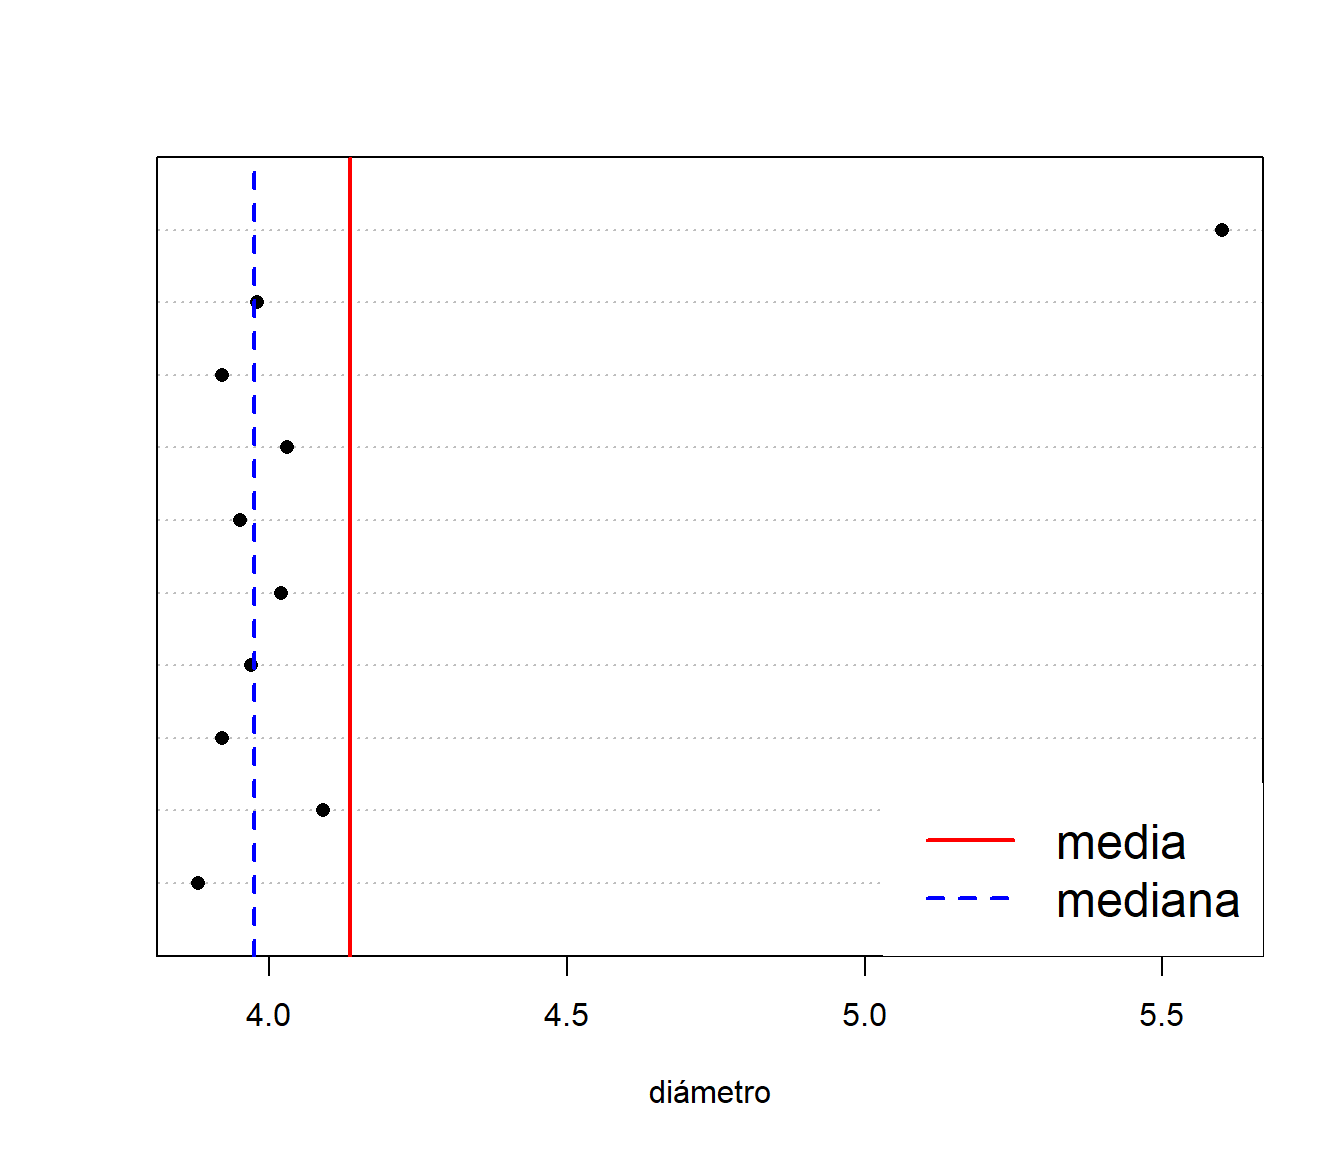
\includegraphics[width=0.7\linewidth]{05-AnalisisExploratorio_files/figure-latex/unnamed-chunk-15-1} \end{center}

Podemos comprobar que la variable \emph{salario} presenta una asimetría
derecha

\begin{Shaded}
\begin{Highlighting}[]
\KeywordTok{mean}\NormalTok{(salario); }\KeywordTok{median}\NormalTok{(salario)}
\end{Highlighting}
\end{Shaded}

\begin{verbatim}
## [1] 34419.57
\end{verbatim}

\begin{verbatim}
## [1] 28875
\end{verbatim}

Calculemos cuántos empleados tienen un salario inferior al salario medio

\begin{Shaded}
\begin{Highlighting}[]
\KeywordTok{mean}\NormalTok{(salario }\OperatorTok{<}\StringTok{ }\KeywordTok{mean}\NormalTok{(salario))}
\end{Highlighting}
\end{Shaded}

\begin{verbatim}
## [1] 0.6940928
\end{verbatim}

\begin{Shaded}
\begin{Highlighting}[]
\KeywordTok{paste}\NormalTok{(}\StringTok{'El '}\NormalTok{, }\KeywordTok{round}\NormalTok{(}\DecValTok{100}\OperatorTok{*}\KeywordTok{mean}\NormalTok{(salario }\OperatorTok{<}\StringTok{ }\KeywordTok{mean}\NormalTok{(salario)),}\DecValTok{0}\NormalTok{), }\StringTok{'%'}\NormalTok{,}
      \StringTok{' de los empleados tienen un salario inferior al salario medio'}\NormalTok{, }\DataTypeTok{sep=}\StringTok{''}\NormalTok{)}
\end{Highlighting}
\end{Shaded}

\begin{verbatim}
## [1] "El 69% de los empleados tienen un salario inferior al salario medio"
\end{verbatim}

Como sabemos, la mitad de los empleados tienen un salario inferior a la
mediana

\begin{Shaded}
\begin{Highlighting}[]
\KeywordTok{mean}\NormalTok{(salario }\OperatorTok{<}\StringTok{ }\KeywordTok{median}\NormalTok{(salario))}
\end{Highlighting}
\end{Shaded}

\begin{verbatim}
## [1] 0.5
\end{verbatim}

Los cuantiles son una generalización de la mediana, que se corresponde
con el cuantil de orden 0.5. \emph{R} contempla distintas formas de
calcular los cuantiles

\begin{Shaded}
\begin{Highlighting}[]
\KeywordTok{median}\NormalTok{(}\KeywordTok{c}\NormalTok{(}\DecValTok{1}\NormalTok{,}\DecValTok{2}\NormalTok{,}\DecValTok{3}\NormalTok{,}\DecValTok{4}\NormalTok{))}
\end{Highlighting}
\end{Shaded}

\begin{verbatim}
## [1] 2.5
\end{verbatim}

\begin{Shaded}
\begin{Highlighting}[]
\KeywordTok{quantile}\NormalTok{(}\KeywordTok{c}\NormalTok{(}\DecValTok{1}\NormalTok{,}\DecValTok{2}\NormalTok{,}\DecValTok{3}\NormalTok{,}\DecValTok{4}\NormalTok{),}\FloatTok{0.5}\NormalTok{)}
\end{Highlighting}
\end{Shaded}

\begin{verbatim}
## 50% 
## 2.5
\end{verbatim}

\begin{Shaded}
\begin{Highlighting}[]
\KeywordTok{quantile}\NormalTok{(}\KeywordTok{c}\NormalTok{(}\DecValTok{1}\NormalTok{,}\DecValTok{2}\NormalTok{,}\DecValTok{3}\NormalTok{,}\DecValTok{4}\NormalTok{),}\FloatTok{0.5}\NormalTok{,}\DataTypeTok{type=}\DecValTok{1}\NormalTok{)}
\end{Highlighting}
\end{Shaded}

\begin{verbatim}
## 50% 
##   2
\end{verbatim}

Calculemos los \emph{cuartiles} y los \emph{deciles} de la variable
\emph{salario}

\begin{Shaded}
\begin{Highlighting}[]
\KeywordTok{quantile}\NormalTok{(salario)}
\end{Highlighting}
\end{Shaded}

\begin{verbatim}
##       0%      25%      50%      75%     100% 
##  15750.0  24000.0  28875.0  36937.5 135000.0
\end{verbatim}

\begin{Shaded}
\begin{Highlighting}[]
\KeywordTok{quantile}\NormalTok{(salario, }\DataTypeTok{probs=}\KeywordTok{c}\NormalTok{(}\FloatTok{0.25}\NormalTok{,}\FloatTok{0.5}\NormalTok{,}\FloatTok{0.75}\NormalTok{))}
\end{Highlighting}
\end{Shaded}

\begin{verbatim}
##     25%     50%     75% 
## 24000.0 28875.0 36937.5
\end{verbatim}

\begin{Shaded}
\begin{Highlighting}[]
\KeywordTok{quantile}\NormalTok{(salario, }\DataTypeTok{probs=}\KeywordTok{seq}\NormalTok{(}\FloatTok{0.1}\NormalTok{, }\FloatTok{0.9}\NormalTok{, }\FloatTok{0.1}\NormalTok{))}
\end{Highlighting}
\end{Shaded}

\begin{verbatim}
##     10%     20%     30%     40%     50%     60%     70%     80%     90% 
## 21045.0 22950.0 24885.0 26700.0 28875.0 30750.0 34500.0 40920.0 59392.5
\end{verbatim}

El \emph{rango} y el \emph{rango intercuartílico}

\begin{Shaded}
\begin{Highlighting}[]
\KeywordTok{data.frame}\NormalTok{(}\DataTypeTok{Rango=}\KeywordTok{max}\NormalTok{(salario)}\OperatorTok{-}\KeywordTok{min}\NormalTok{(salario),}
           \DataTypeTok{RI=}\KeywordTok{as.numeric}\NormalTok{(}\KeywordTok{quantile}\NormalTok{(salario, }\FloatTok{0.75}\NormalTok{) }\OperatorTok{-}\StringTok{ }\KeywordTok{quantile}\NormalTok{(salario, }\FloatTok{0.25}\NormalTok{)))}
\end{Highlighting}
\end{Shaded}

\begin{verbatim}
##    Rango      RI
## 1 119250 12937.5
\end{verbatim}

\subsection{\texorpdfstring{\emph{Summary}}{Summary}}\label{summary}

\begin{Shaded}
\begin{Highlighting}[]
\KeywordTok{summary}\NormalTok{(empleados)}
\end{Highlighting}
\end{Shaded}

\begin{verbatim}
##        id            sexo        fechnac                educ      
##  Min.   :  1.0   Hombre:258   Min.   :1929-02-10   Min.   : 8.00  
##  1st Qu.:119.2   Mujer :216   1st Qu.:1948-01-03   1st Qu.:12.00  
##  Median :237.5                Median :1962-01-23   Median :12.00  
##  Mean   :237.5                Mean   :1956-10-08   Mean   :13.49  
##  3rd Qu.:355.8                3rd Qu.:1965-07-06   3rd Qu.:15.00  
##  Max.   :474.0                Max.   :1971-02-10   Max.   :21.00  
##                               NA's   :1                           
##             catlab       salario           salini         tiempemp    
##  Administrativo:363   Min.   : 15750   Min.   : 9000   Min.   :63.00  
##  Seguridad     : 27   1st Qu.: 24000   1st Qu.:12488   1st Qu.:72.00  
##  Directivo     : 84   Median : 28875   Median :15000   Median :81.00  
##                       Mean   : 34420   Mean   :17016   Mean   :81.11  
##                       3rd Qu.: 36938   3rd Qu.:17490   3rd Qu.:90.00  
##                       Max.   :135000   Max.   :79980   Max.   :98.00  
##                                                                       
##     expprev       minoria           sexoraza  
##  Min.   :  0.00   No:370   Blanca varón :194  
##  1st Qu.: 19.25   Sí:104   Minoría varón: 64  
##  Median : 55.00            Blanca mujer :176  
##  Mean   : 95.86            Minoría mujer: 40  
##  3rd Qu.:138.75                               
##  Max.   :476.00                               
## 
\end{verbatim}

\begin{Shaded}
\begin{Highlighting}[]
\KeywordTok{summary}\NormalTok{(}\KeywordTok{subset}\NormalTok{(empleados,catlab}\OperatorTok{==}\StringTok{'Directivo'}\NormalTok{))}
\end{Highlighting}
\end{Shaded}

\begin{verbatim}
##        id            sexo       fechnac                educ      
##  Min.   :  1.0   Hombre:74   Min.   :1937-07-12   Min.   :12.00  
##  1st Qu.:102.5   Mujer :10   1st Qu.:1954-08-09   1st Qu.:16.00  
##  Median :233.5               Median :1961-05-29   Median :17.00  
##  Mean   :234.1               Mean   :1958-11-26   Mean   :17.25  
##  3rd Qu.:344.2               3rd Qu.:1963-10-03   3rd Qu.:19.00  
##  Max.   :468.0               Max.   :1966-04-05   Max.   :21.00  
##             catlab      salario           salini         tiempemp    
##  Administrativo: 0   Min.   : 34410   Min.   :15750   Min.   :64.00  
##  Seguridad     : 0   1st Qu.: 51956   1st Qu.:23063   1st Qu.:73.00  
##  Directivo     :84   Median : 60500   Median :28740   Median :81.00  
##                      Mean   : 63978   Mean   :30258   Mean   :81.15  
##                      3rd Qu.: 71281   3rd Qu.:34058   3rd Qu.:91.00  
##                      Max.   :135000   Max.   :79980   Max.   :98.00  
##     expprev       minoria          sexoraza 
##  Min.   :  3.00   No:80   Blanca varón :70  
##  1st Qu.: 19.75   Sí: 4   Minoría varón: 4  
##  Median : 52.00           Blanca mujer :10  
##  Mean   : 77.62           Minoría mujer: 0  
##  3rd Qu.:125.25                             
##  Max.   :285.00
\end{verbatim}

\section{Gráficos}\label{graficos-1}

\subsection{Diagrama de barras y gráfico de
sectores}\label{diagrama-de-barras-y-grafico-de-sectores}

\begin{Shaded}
\begin{Highlighting}[]
\KeywordTok{table}\NormalTok{(catlab)}
\end{Highlighting}
\end{Shaded}

\begin{verbatim}
## catlab
## Administrativo      Seguridad      Directivo 
##            363             27             84
\end{verbatim}

\begin{Shaded}
\begin{Highlighting}[]
\KeywordTok{par}\NormalTok{(}\DataTypeTok{mfrow =} \KeywordTok{c}\NormalTok{(}\DecValTok{1}\NormalTok{, }\DecValTok{3}\NormalTok{))}
\KeywordTok{barplot}\NormalTok{(}\KeywordTok{table}\NormalTok{(catlab),}\DataTypeTok{main=}\StringTok{"frecuencia absoluta"}\NormalTok{)}
\KeywordTok{barplot}\NormalTok{(}\DecValTok{100}\OperatorTok{*}\KeywordTok{prop.table}\NormalTok{(}\KeywordTok{table}\NormalTok{(catlab)),}\DataTypeTok{main=}\StringTok{"frecuencia relativa (%)"}\NormalTok{)}
\KeywordTok{pie}\NormalTok{(}\KeywordTok{table}\NormalTok{(catlab))}
\end{Highlighting}
\end{Shaded}

\begin{center}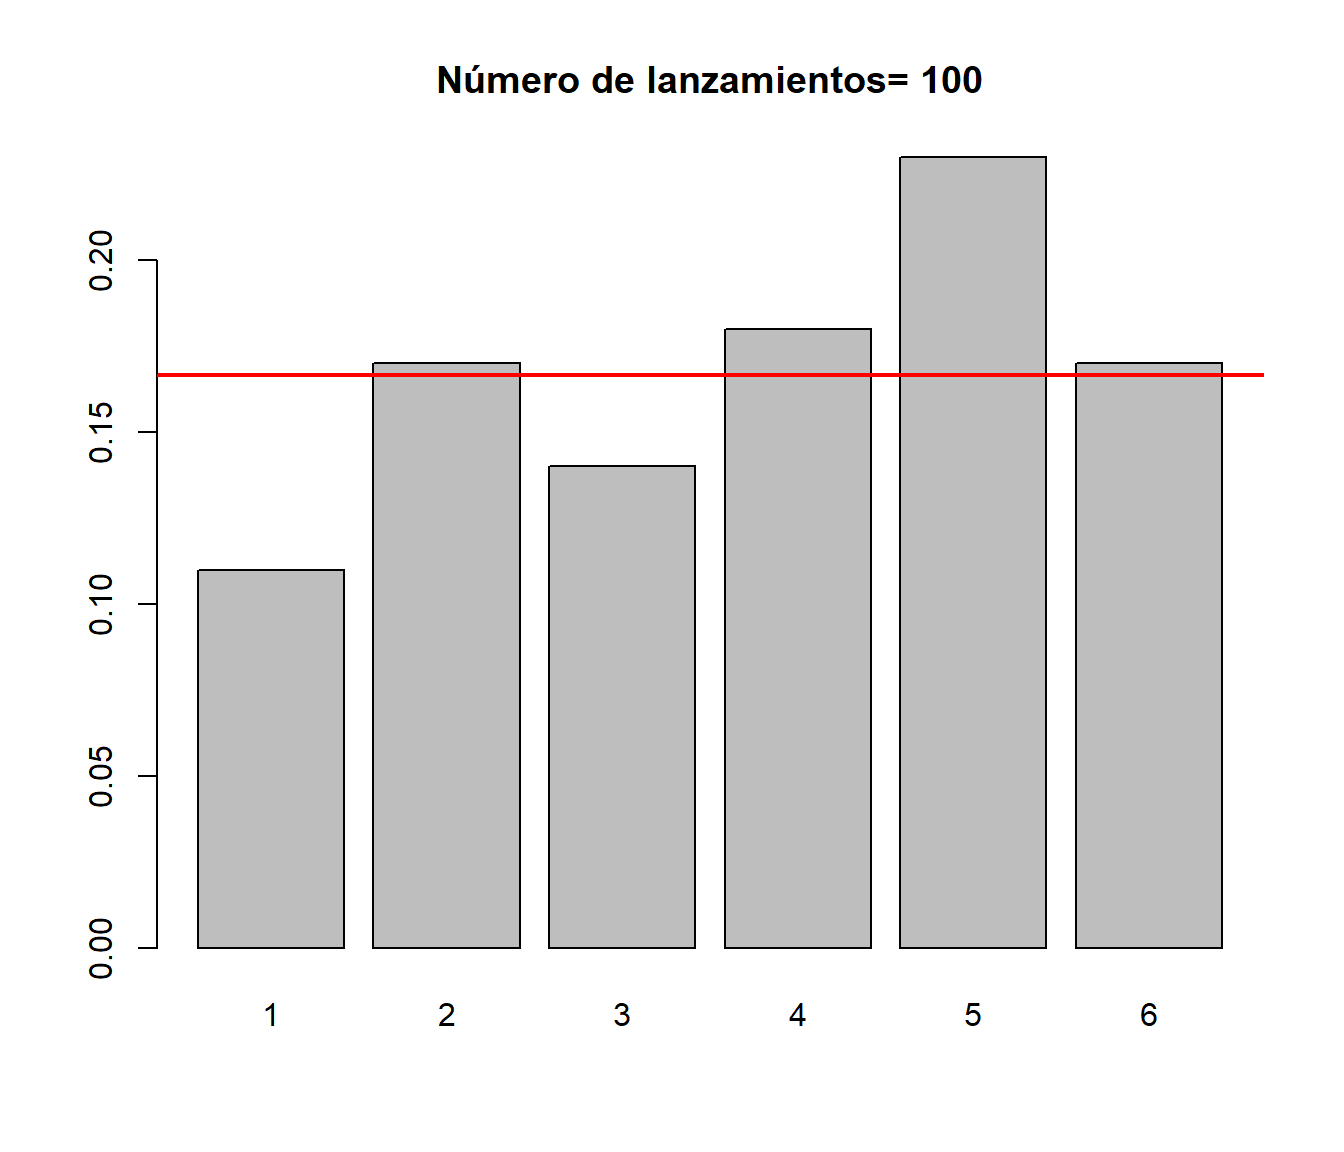
\includegraphics[width=0.7\linewidth]{05-AnalisisExploratorio_files/figure-latex/unnamed-chunk-23-1} \end{center}

\begin{Shaded}
\begin{Highlighting}[]
\NormalTok{nj <-}\StringTok{ }\KeywordTok{table}\NormalTok{(educ)}
\NormalTok{fj <-}\StringTok{ }\KeywordTok{prop.table}\NormalTok{(nj)}
\NormalTok{Nj <-}\StringTok{ }\KeywordTok{cumsum}\NormalTok{(nj)}
\NormalTok{Fj <-}\StringTok{ }\KeywordTok{cumsum}\NormalTok{(fj)}
\KeywordTok{layout}\NormalTok{(}\KeywordTok{matrix}\NormalTok{(}\KeywordTok{c}\NormalTok{(}\DecValTok{1}\NormalTok{,}\DecValTok{2}\NormalTok{,}\DecValTok{5}\NormalTok{,}\DecValTok{3}\NormalTok{,}\DecValTok{4}\NormalTok{,}\DecValTok{5}\NormalTok{), }\DecValTok{2}\NormalTok{, }\DecValTok{3}\NormalTok{, }\DataTypeTok{byrow=}\OtherTok{TRUE}\NormalTok{), }\DataTypeTok{respect=}\OtherTok{TRUE}\NormalTok{)}
\KeywordTok{barplot}\NormalTok{(nj,}\DataTypeTok{main=}\StringTok{"frecuencia absolutas"}\NormalTok{,}\DataTypeTok{xlab=}\StringTok{'años de estudio'}\NormalTok{)}
\KeywordTok{barplot}\NormalTok{(fj,}\DataTypeTok{main=}\StringTok{"frecuencia relativas"}\NormalTok{,}\DataTypeTok{xlab=}\StringTok{'años de estudio'}\NormalTok{)}
\KeywordTok{barplot}\NormalTok{(Nj,}\DataTypeTok{main=}\StringTok{"frecuencia absolutas acumuladas"}\NormalTok{,}\DataTypeTok{xlab=}\StringTok{'años de estudio'}\NormalTok{)}
\KeywordTok{barplot}\NormalTok{(Fj,}\DataTypeTok{main=}\StringTok{"frecuencia relativas acumuladas"}\NormalTok{,}\DataTypeTok{xlab=}\StringTok{'años de estudio'}\NormalTok{)}
\KeywordTok{pie}\NormalTok{(nj,}\DataTypeTok{col=}\KeywordTok{rainbow}\NormalTok{(}\DecValTok{6}\NormalTok{),}\DataTypeTok{main=}\StringTok{'años de estudio'}\NormalTok{)}
\end{Highlighting}
\end{Shaded}

\begin{center}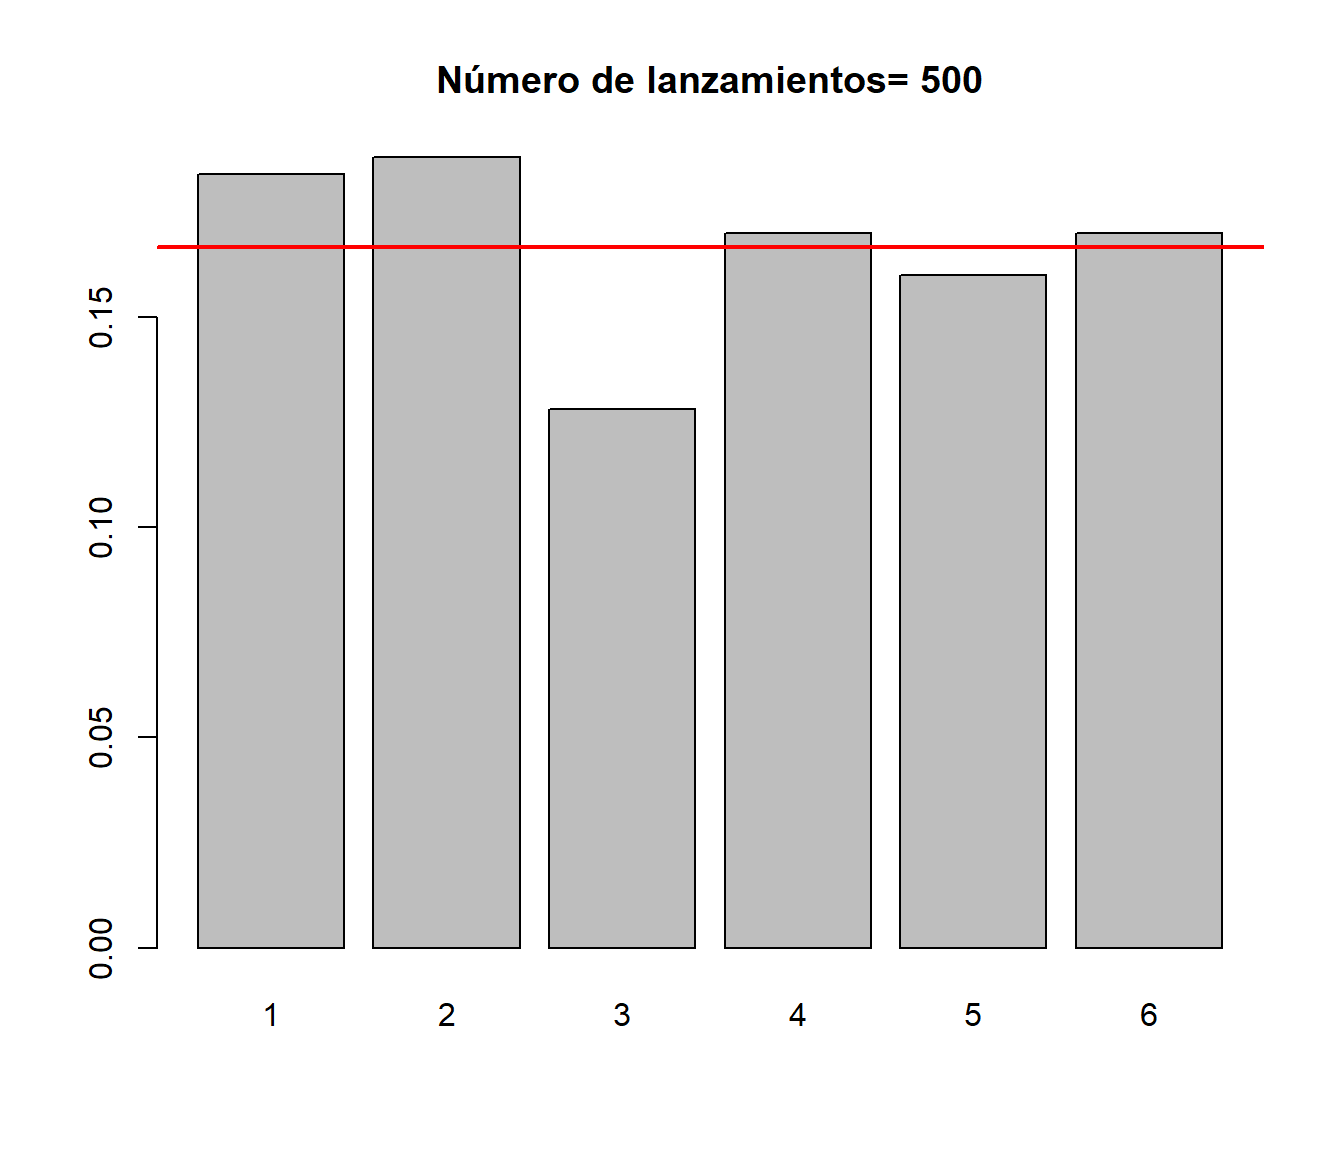
\includegraphics[width=0.7\linewidth]{05-AnalisisExploratorio_files/figure-latex/unnamed-chunk-23-2} \end{center}

\begin{Shaded}
\begin{Highlighting}[]
\KeywordTok{par}\NormalTok{(}\DataTypeTok{mfrow =} \KeywordTok{c}\NormalTok{(}\DecValTok{1}\NormalTok{, }\DecValTok{1}\NormalTok{))}
\end{Highlighting}
\end{Shaded}

Con datos continuos, podemos hacer uso de la función \emph{cut} (más
adelante veremos como se representa el histograma)

\begin{Shaded}
\begin{Highlighting}[]
\KeywordTok{table}\NormalTok{(}\KeywordTok{cut}\NormalTok{(expprev, }\DataTypeTok{breaks=}\DecValTok{5}\NormalTok{))}
\end{Highlighting}
\end{Shaded}

\begin{verbatim}
## 
## (-0.476,95.2]    (95.2,190]     (190,286]     (286,381]     (381,476] 
##           312            81            46            22            13
\end{verbatim}

\begin{Shaded}
\begin{Highlighting}[]
\KeywordTok{barplot}\NormalTok{(}\KeywordTok{table}\NormalTok{(}\KeywordTok{cut}\NormalTok{(expprev,}\DataTypeTok{breaks=}\DecValTok{5}\NormalTok{)),}\DataTypeTok{xlab=}\StringTok{"Experiencia previa"}\NormalTok{,}
        \DataTypeTok{main=}\StringTok{"Categorización en 5 clases"}\NormalTok{)}
\end{Highlighting}
\end{Shaded}

\begin{center}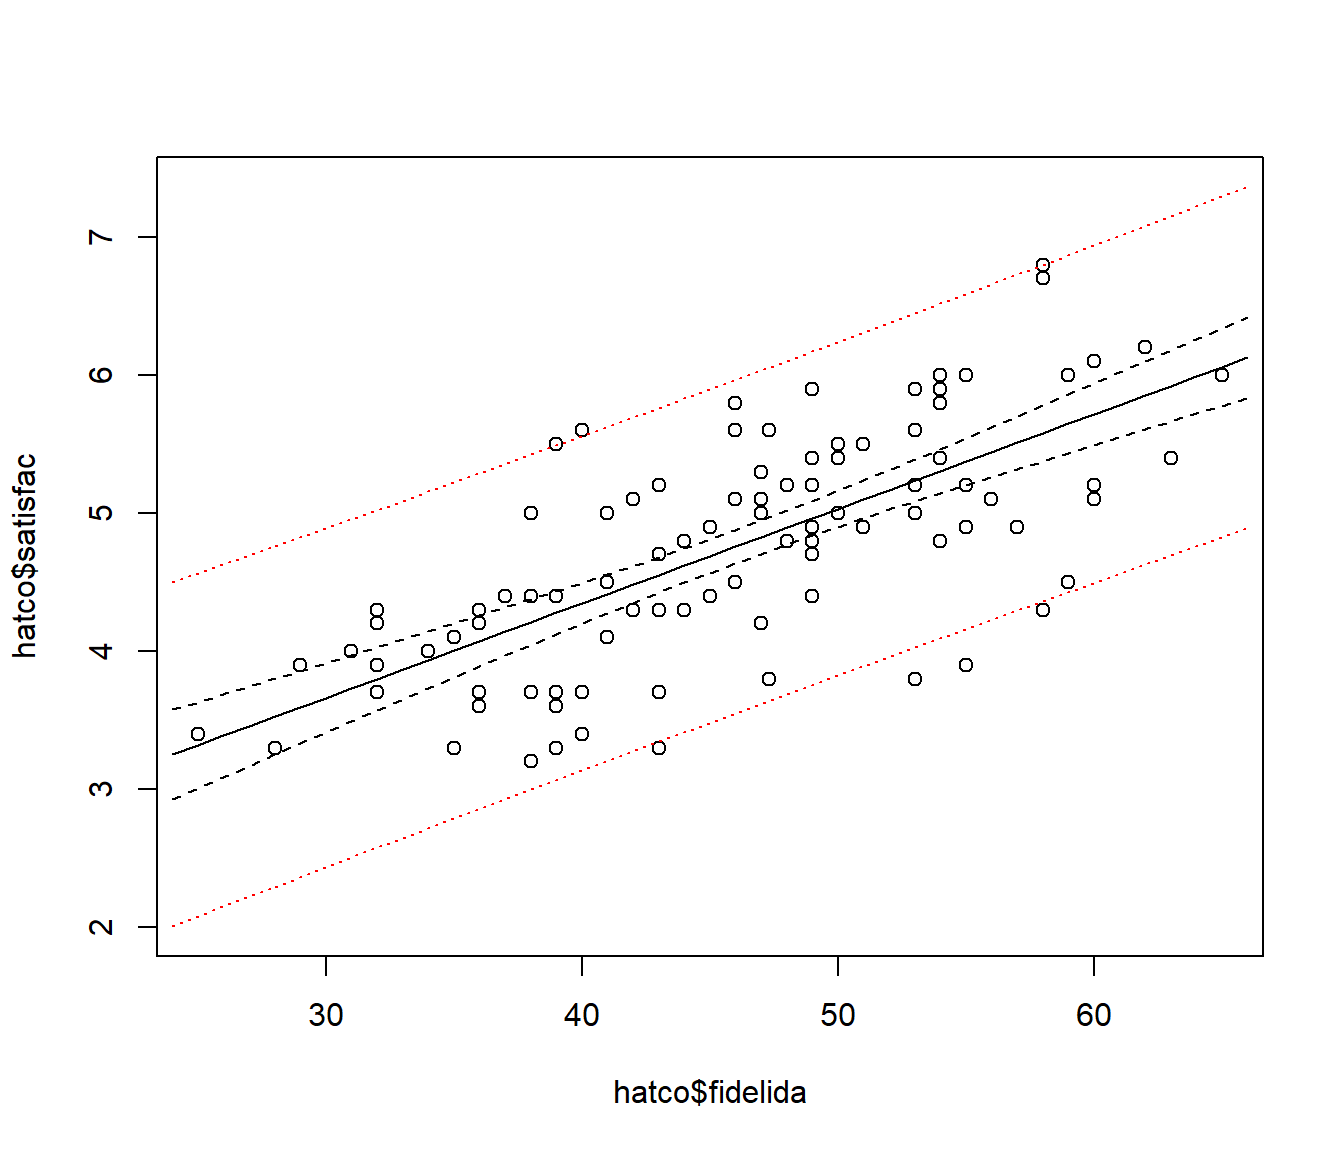
\includegraphics[width=0.7\linewidth]{05-AnalisisExploratorio_files/figure-latex/unnamed-chunk-24-1} \end{center}

Debemos ser muy cuidadosos a la hora de valorar gráficas como la
siguiente

\begin{Shaded}
\begin{Highlighting}[]
\NormalTok{tt <-}\StringTok{ }\KeywordTok{table}\NormalTok{(}\KeywordTok{cut}\NormalTok{(expprev, }\DataTypeTok{breaks=}\KeywordTok{c}\NormalTok{(}\DecValTok{0}\NormalTok{,}\DecValTok{40}\NormalTok{,}\DecValTok{80}\NormalTok{,}\DecValTok{150}\NormalTok{,}\DecValTok{250}\NormalTok{,}\DecValTok{400}\NormalTok{)))}
\KeywordTok{barplot}\NormalTok{(tt,}\DataTypeTok{xlab=}\StringTok{"Experiencia previa"}\NormalTok{, }\DataTypeTok{main=}\StringTok{"Categorización en 5 clases"}\NormalTok{)}
\end{Highlighting}
\end{Shaded}

\begin{center}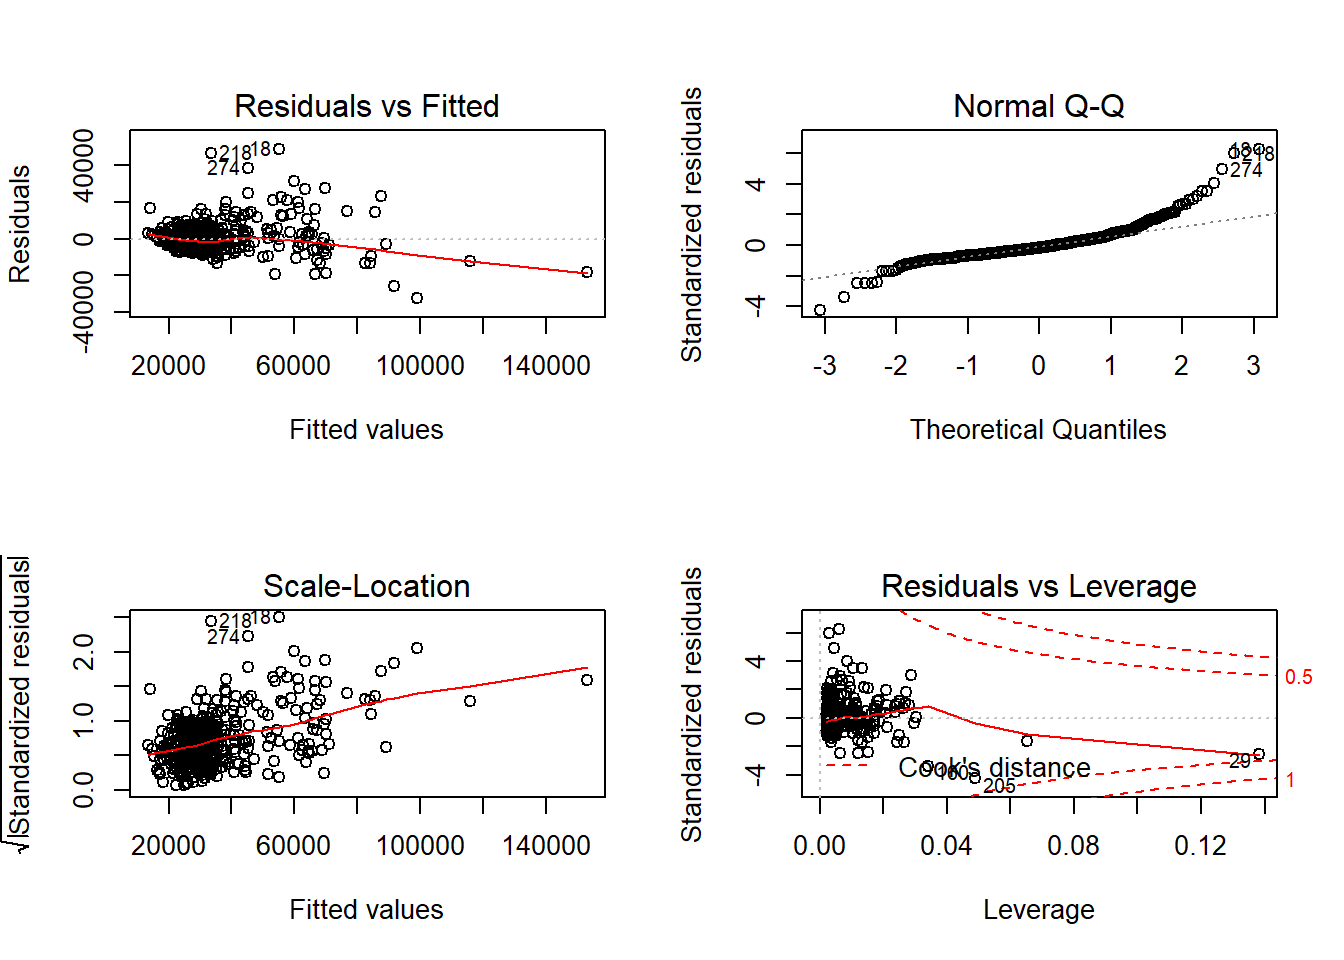
\includegraphics[width=0.7\linewidth]{05-AnalisisExploratorio_files/figure-latex/unnamed-chunk-25-1} \end{center}

\subsection{Gráfico de puntos}\label{grafico-de-puntos}

\begin{Shaded}
\begin{Highlighting}[]
\KeywordTok{dotchart}\NormalTok{(salario, }\DataTypeTok{xlab=}\StringTok{'salarios'}\NormalTok{)}
\end{Highlighting}
\end{Shaded}

\begin{center}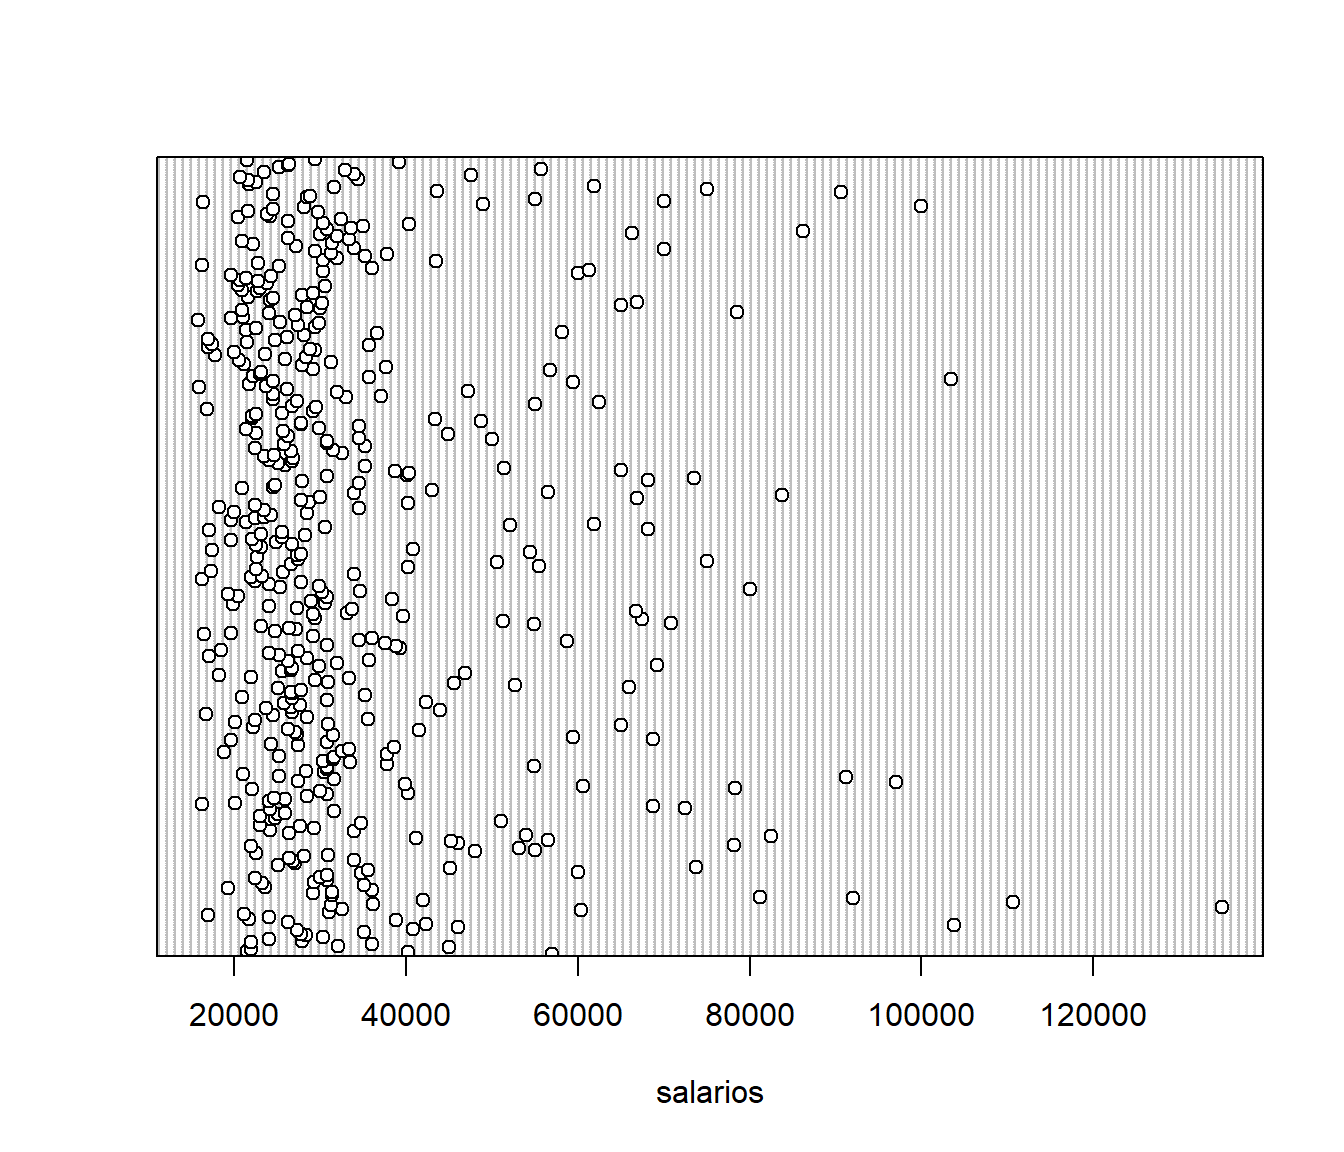
\includegraphics[width=0.7\linewidth]{05-AnalisisExploratorio_files/figure-latex/unnamed-chunk-26-1} \end{center}

\begin{Shaded}
\begin{Highlighting}[]
\KeywordTok{stripchart}\NormalTok{(salario}\OperatorTok{~}\NormalTok{sexo, }\DataTypeTok{method=}\StringTok{'jitter'}\NormalTok{)}
\end{Highlighting}
\end{Shaded}

\begin{center}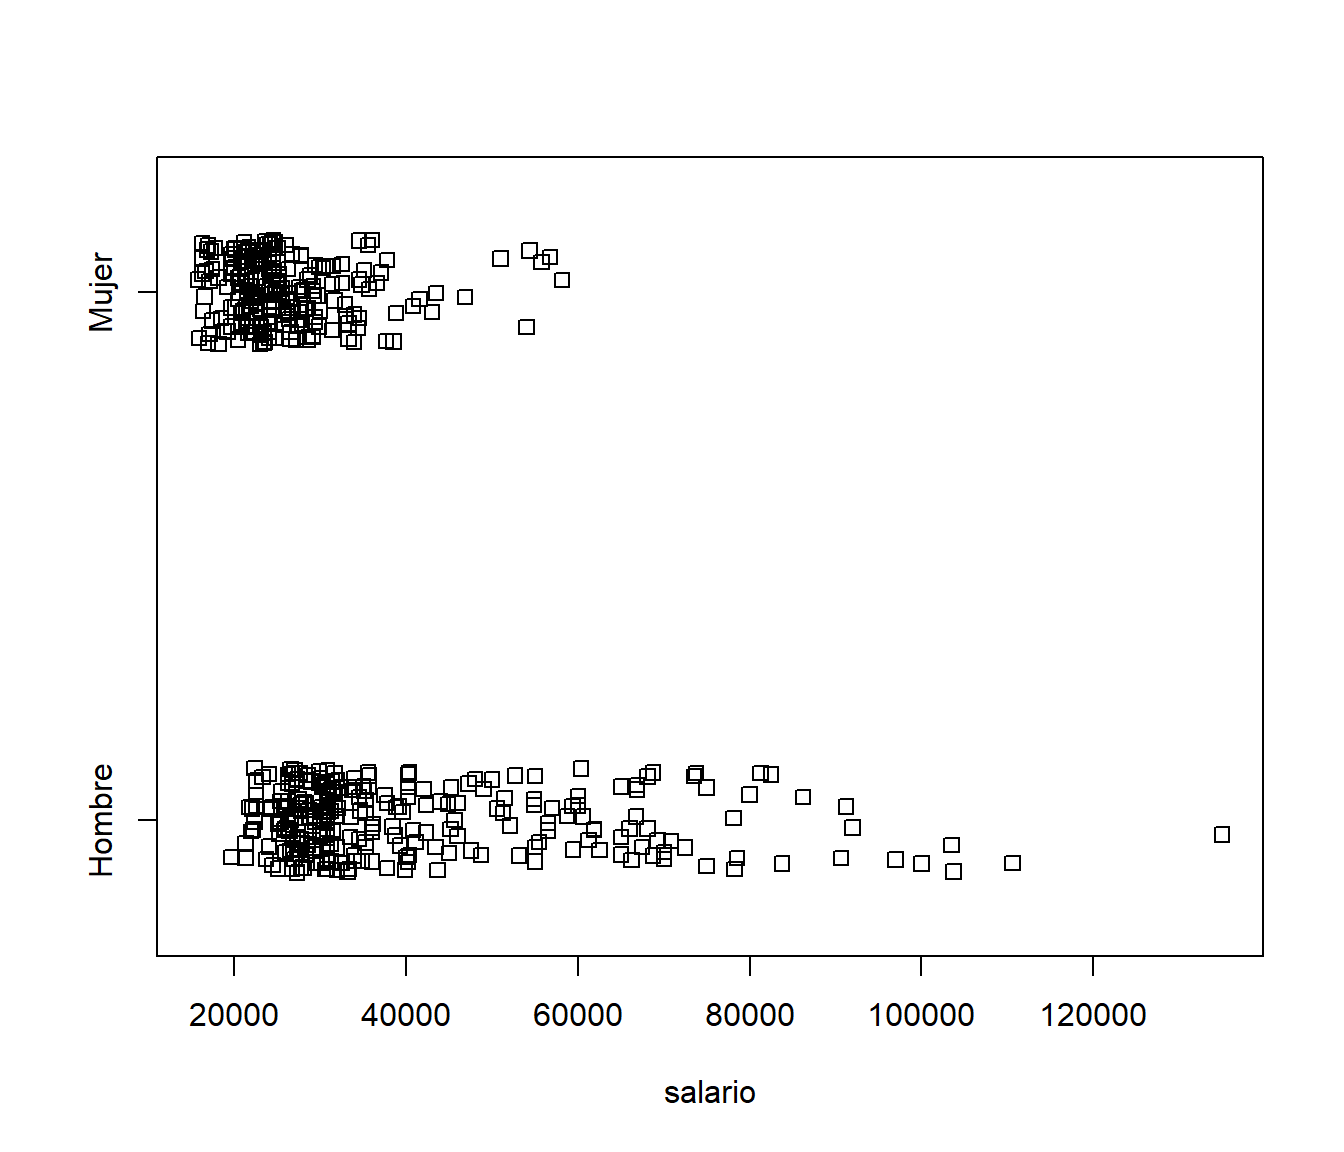
\includegraphics[width=0.7\linewidth]{05-AnalisisExploratorio_files/figure-latex/unnamed-chunk-26-2} \end{center}

\subsection{Árbol de tallo y hojas}\label{arbol-de-tallo-y-hojas}

Esta representación puede ser útil cuando se dispone de pocos datos.

\begin{Shaded}
\begin{Highlighting}[]
\KeywordTok{stem}\NormalTok{(salario)}
\end{Highlighting}
\end{Shaded}

\begin{verbatim}
## 
##   The decimal point is 4 digit(s) to the right of the |
## 
##    1 | 666666777777777778888999
##    2 | 00000000000000111111111111111111122222222222222222222222233333333333+148
##    3 | 00000000000000000001111111111111111111111111122222222222223333333333+36
##    4 | 0000000001112222334445555666778899
##    5 | 0111123344555556677778999
##    6 | 0001122355566777888999
##    7 | 00134455889
##    8 | 01346
##    9 | 1127
##   10 | 044
##   11 | 1
##   12 | 
##   13 | 5
\end{verbatim}

\begin{Shaded}
\begin{Highlighting}[]
\KeywordTok{stem}\NormalTok{(tiempemp)}
\end{Highlighting}
\end{Shaded}

\begin{verbatim}
## 
##   The decimal point is at the |
## 
##   62 | 000
##   64 | 00000000000000000000000
##   66 | 000000000000000000000000000000000
##   68 | 0000000000000000000000000000000
##   70 | 0000000000000000
##   72 | 00000000000000000000000000
##   74 | 000000000000000
##   76 | 00000000000000000000000
##   78 | 000000000000000000000000000000000000
##   80 | 00000000000000000000000000000000000000
##   82 | 0000000000000000000000000000000000
##   84 | 000000000000000000000000
##   86 | 000000000000000000000000
##   88 | 00000000000000000000
##   90 | 00000000000000000000000000000
##   92 | 00000000000000000000000000000000000000
##   94 | 00000000000000000000
##   96 | 000000000000000000000000000
##   98 | 00000000000000
\end{verbatim}

\subsection{Histograma}\label{histograma}

Este gráfico es uno de los más habituales para representar datos
continuos

\begin{Shaded}
\begin{Highlighting}[]
\KeywordTok{hist}\NormalTok{(salario, }\DataTypeTok{main=}\StringTok{'número de clases por defecto'}\NormalTok{)}
\end{Highlighting}
\end{Shaded}

\begin{center}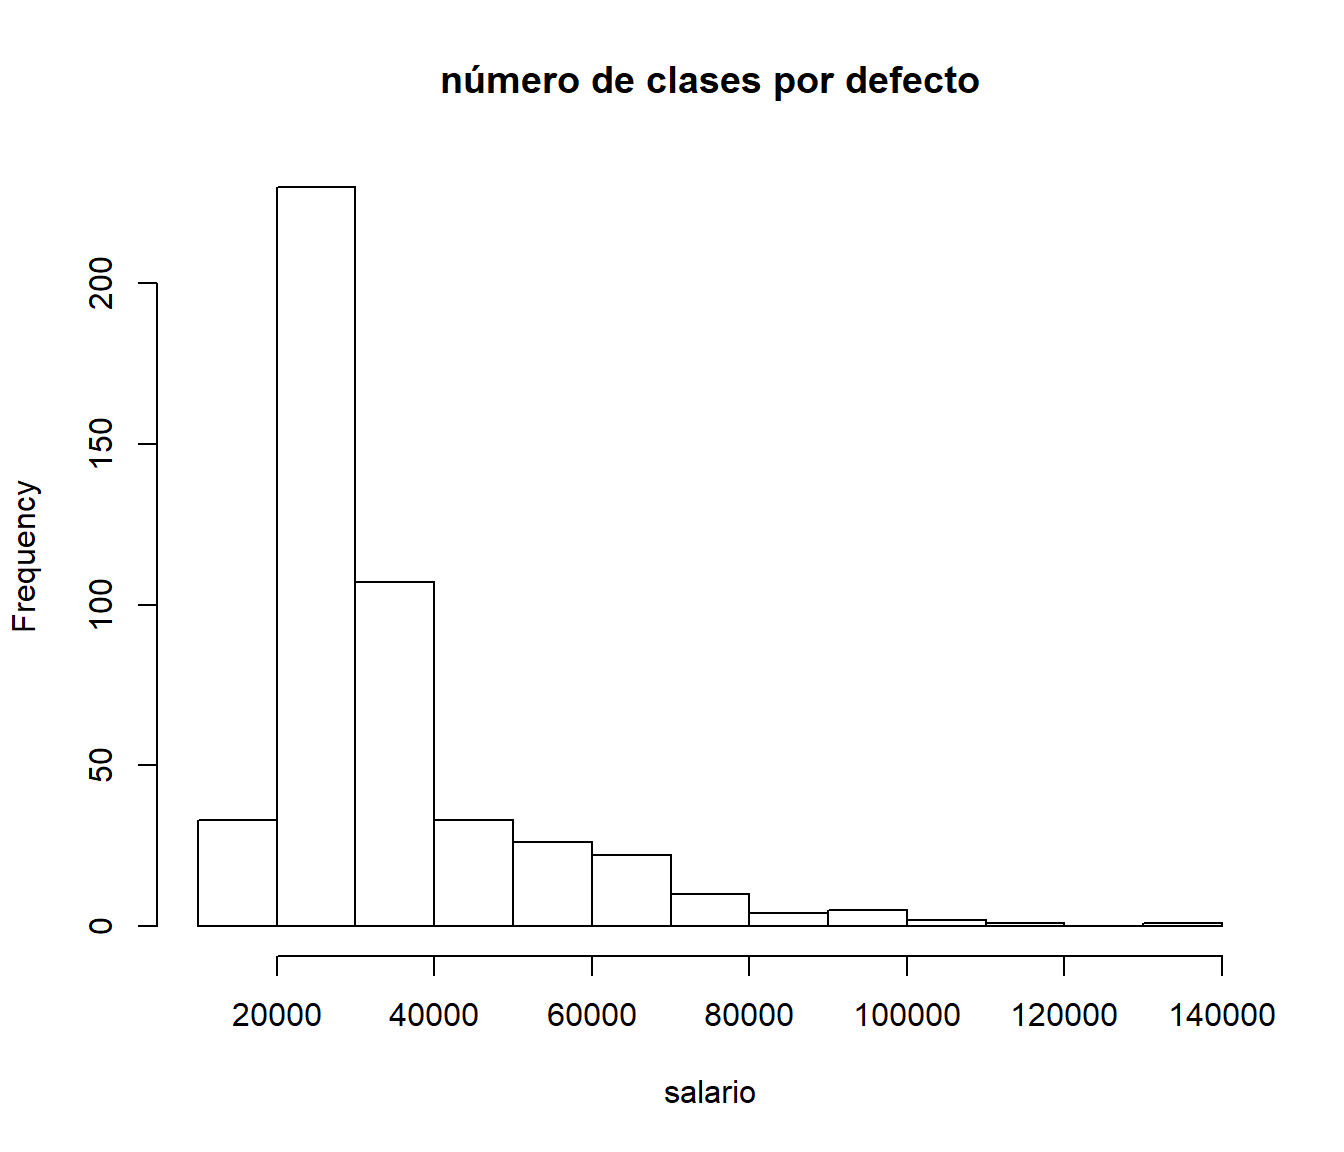
\includegraphics[width=0.7\linewidth]{05-AnalisisExploratorio_files/figure-latex/unnamed-chunk-28-1} \end{center}

\begin{Shaded}
\begin{Highlighting}[]
\KeywordTok{hist}\NormalTok{(salario, }\DataTypeTok{breaks=}\DecValTok{3}\NormalTok{, }\DataTypeTok{main=}\StringTok{'3 intervalos de clase'}\NormalTok{)}
\end{Highlighting}
\end{Shaded}

\begin{center}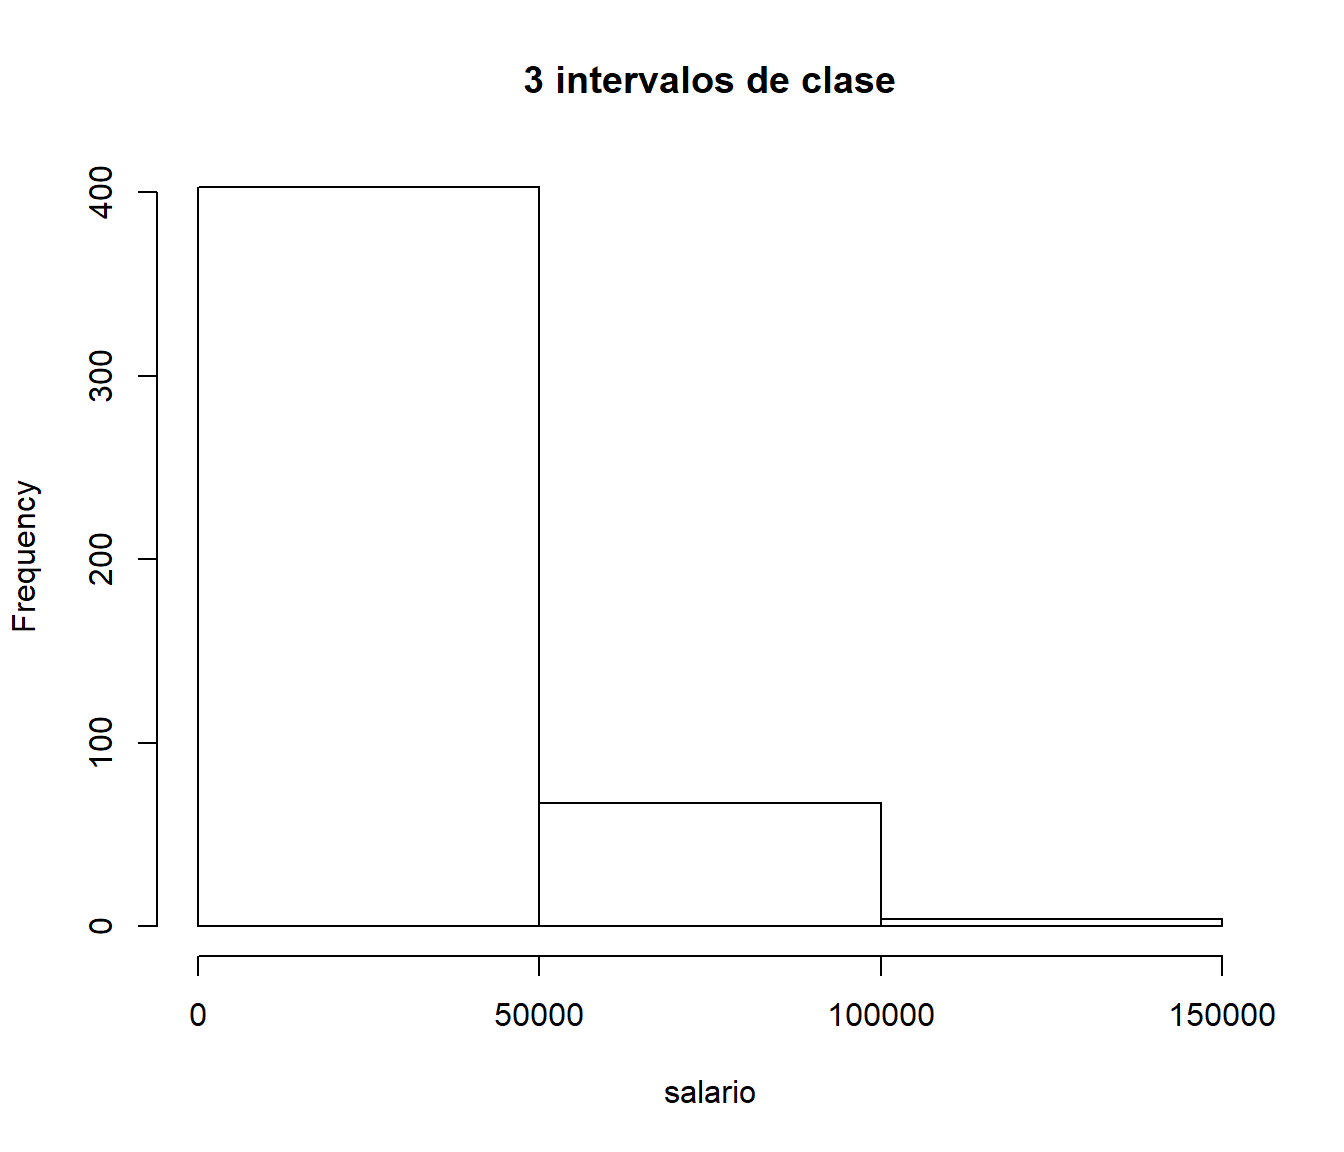
\includegraphics[width=0.7\linewidth]{05-AnalisisExploratorio_files/figure-latex/unnamed-chunk-28-2} \end{center}

\begin{Shaded}
\begin{Highlighting}[]
\KeywordTok{hist}\NormalTok{(salario, }\DataTypeTok{breaks=}\DecValTok{100}\NormalTok{, }\DataTypeTok{main=}\StringTok{'100 intervalos de clase'}\NormalTok{)}
\end{Highlighting}
\end{Shaded}

\begin{center}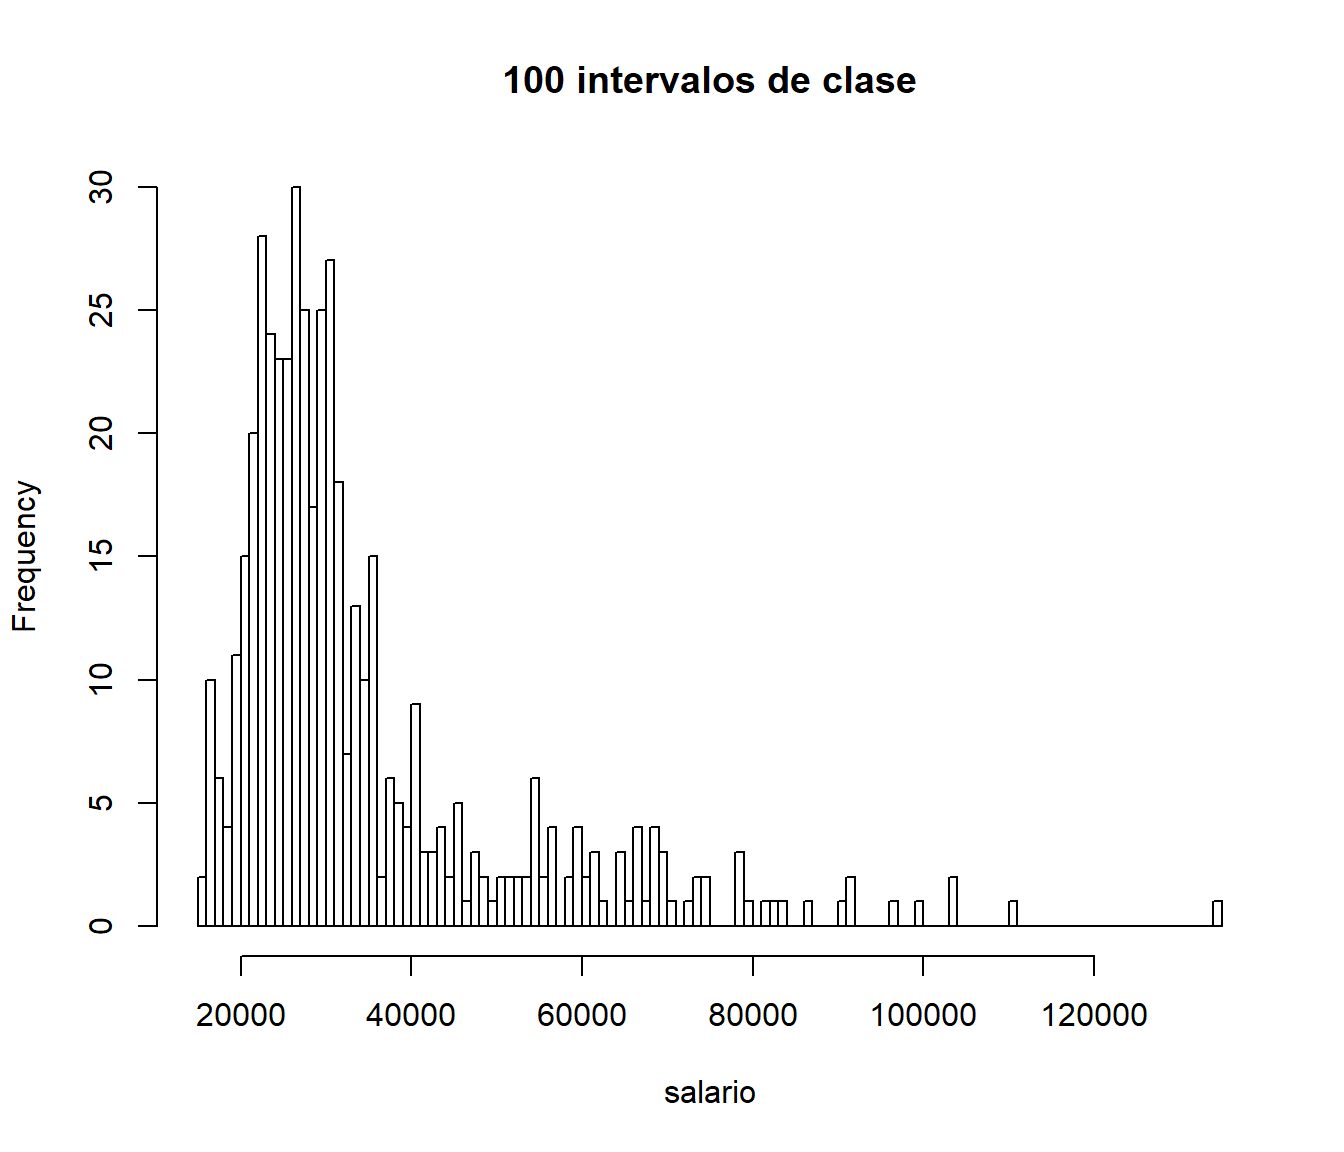
\includegraphics[width=0.7\linewidth]{05-AnalisisExploratorio_files/figure-latex/unnamed-chunk-28-3} \end{center}

\begin{Shaded}
\begin{Highlighting}[]
\NormalTok{cl1 <-}\StringTok{ }\KeywordTok{seq}\NormalTok{(}\DecValTok{15000}\NormalTok{,}\DecValTok{40000}\NormalTok{,}\DecValTok{5000}\NormalTok{)}
\NormalTok{cl2 <-}\StringTok{ }\KeywordTok{seq}\NormalTok{(}\DecValTok{50000}\NormalTok{,}\DecValTok{80000}\NormalTok{,}\DecValTok{10000}\NormalTok{)}
\NormalTok{cl3 <-}\StringTok{ }\KeywordTok{seq}\NormalTok{(}\DecValTok{100000}\NormalTok{,}\DecValTok{140000}\NormalTok{,}\DecValTok{20000}\NormalTok{)}
\KeywordTok{hist}\NormalTok{(salario, }\DataTypeTok{breaks=}\KeywordTok{c}\NormalTok{(cl1,cl2,cl3),}\DataTypeTok{main=}\StringTok{'intervalos de clase de distinta amplitud'}\NormalTok{)}
\end{Highlighting}
\end{Shaded}

\begin{center}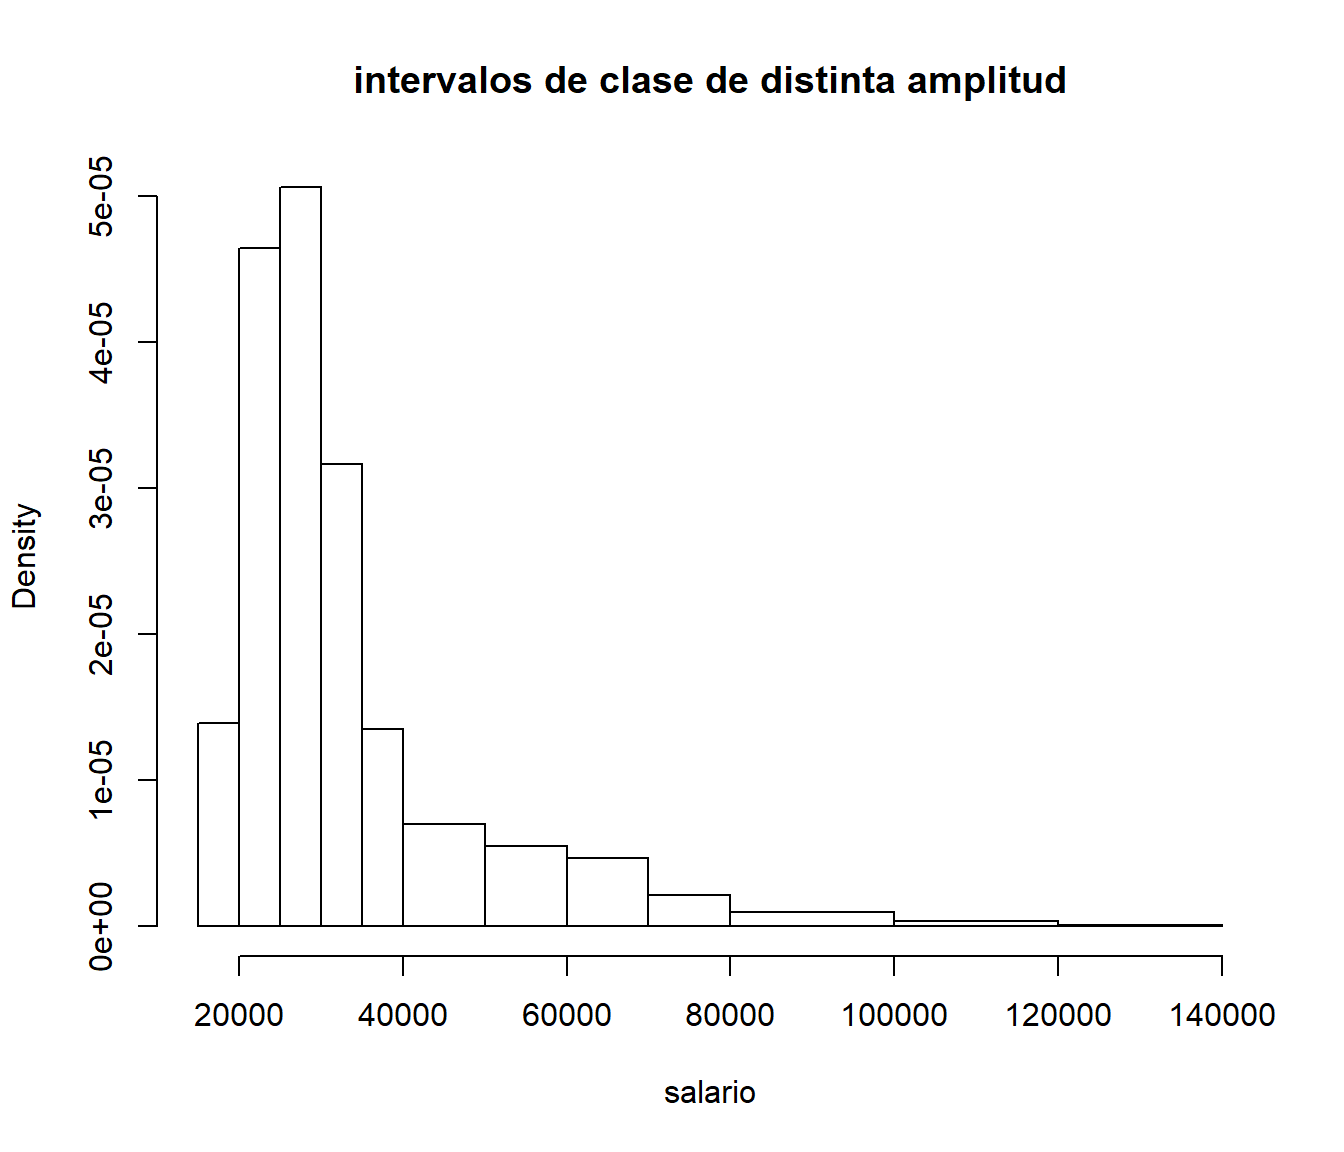
\includegraphics[width=0.7\linewidth]{05-AnalisisExploratorio_files/figure-latex/unnamed-chunk-28-4} \end{center}

\subsection{Gráfico de densidad}\label{grafico-de-densidad}

Es una versión suavizada del histograma.

\begin{Shaded}
\begin{Highlighting}[]
\KeywordTok{plot}\NormalTok{(}\KeywordTok{density}\NormalTok{(salario))}
\end{Highlighting}
\end{Shaded}

\begin{center}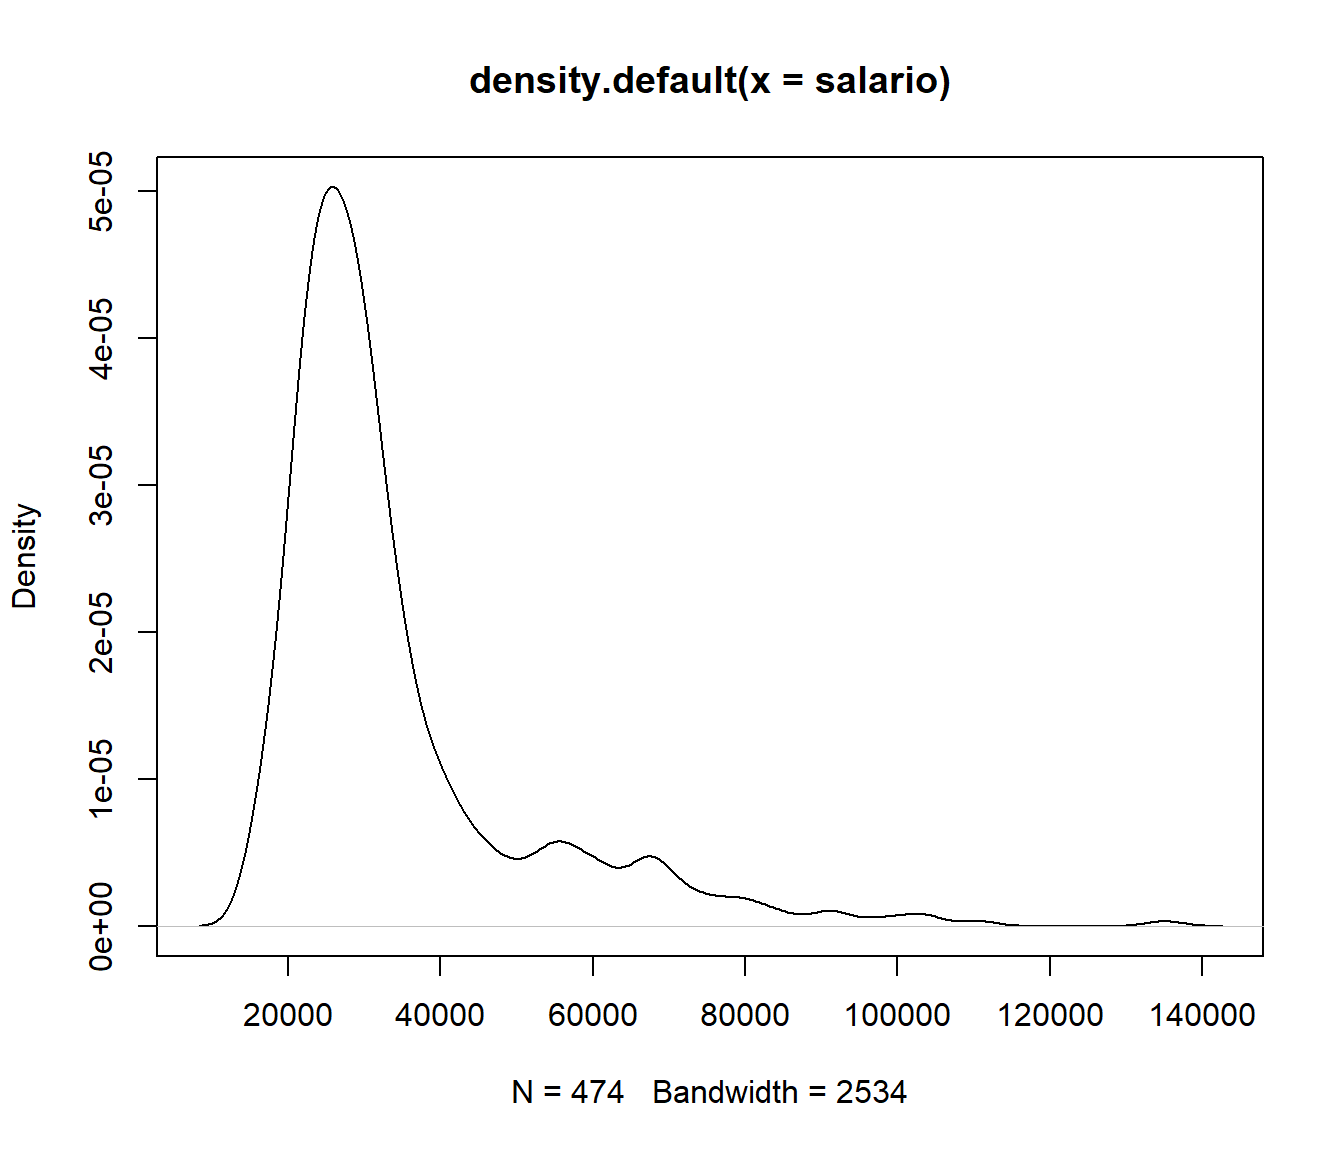
\includegraphics[width=0.7\linewidth]{05-AnalisisExploratorio_files/figure-latex/unnamed-chunk-29-1} \end{center}

\begin{Shaded}
\begin{Highlighting}[]
\KeywordTok{hist}\NormalTok{(salario, }\DataTypeTok{freq=}\NormalTok{F, }\DataTypeTok{main=}\StringTok{''}\NormalTok{)}
\KeywordTok{lines}\NormalTok{(}\KeywordTok{density}\NormalTok{(salario), }\DataTypeTok{lwd=}\DecValTok{3}\NormalTok{, }\DataTypeTok{col=}\StringTok{'red'}\NormalTok{)}
\end{Highlighting}
\end{Shaded}

\begin{center}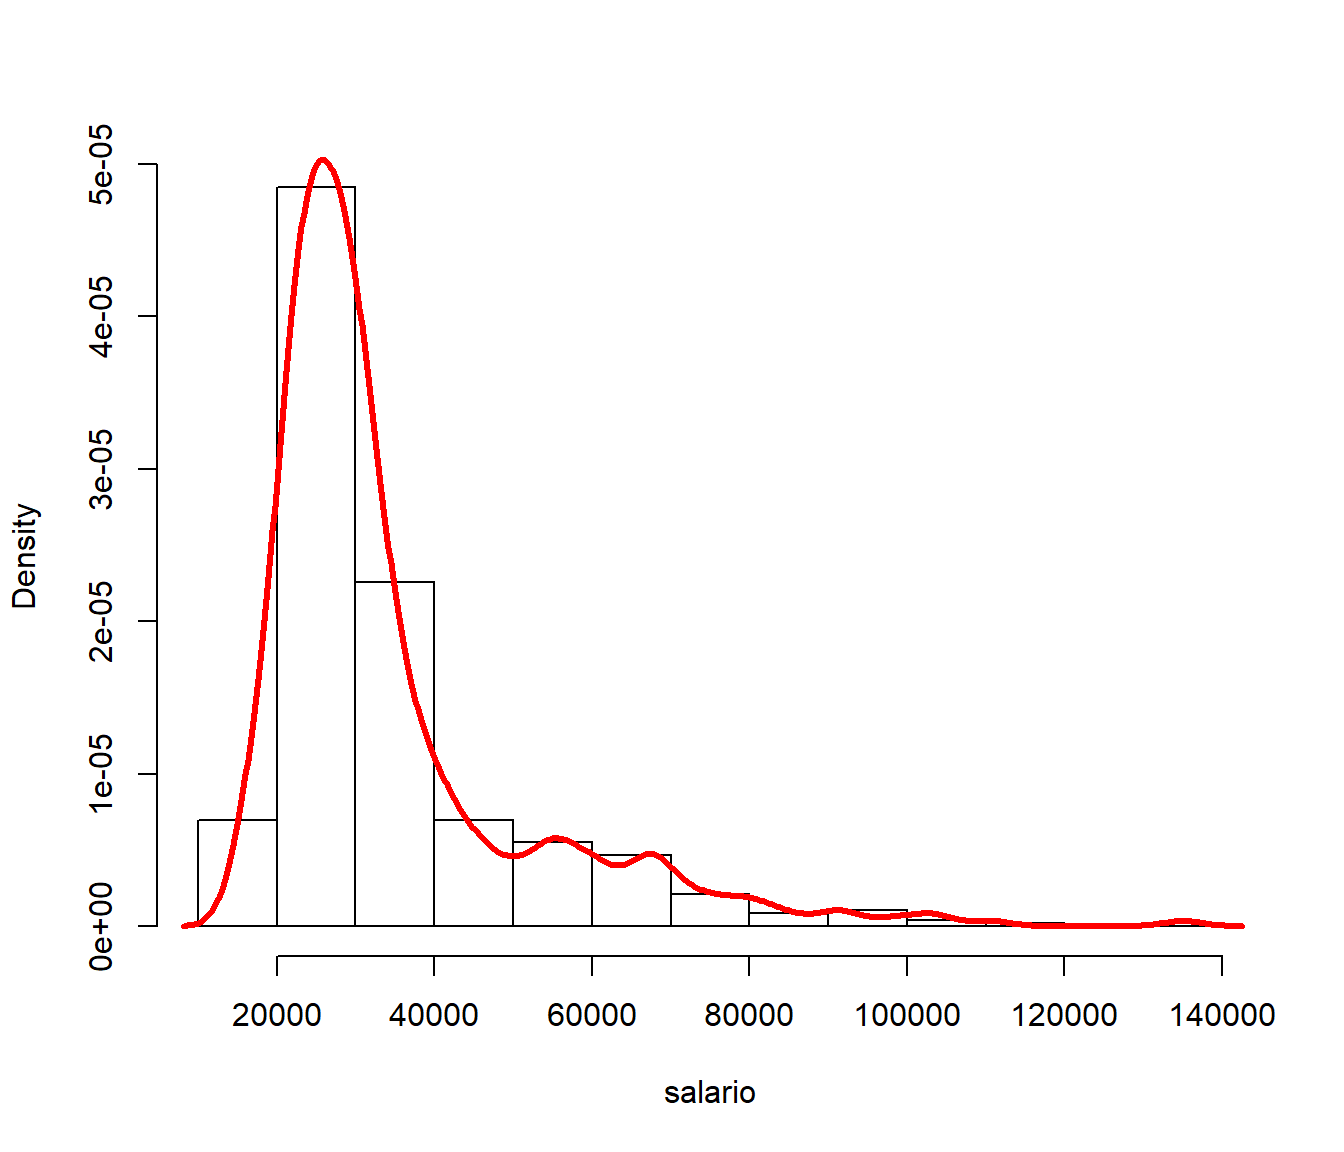
\includegraphics[width=0.7\linewidth]{05-AnalisisExploratorio_files/figure-latex/unnamed-chunk-29-2} \end{center}

El paquete \emph{car} nos da acceso a la instrucción \emph{densityPlot}:

\begin{Shaded}
\begin{Highlighting}[]
\KeywordTok{library}\NormalTok{(car)  }\CommentTok{# help(car)}
\KeywordTok{densityPlot}\NormalTok{(salario}\OperatorTok{~}\NormalTok{sexo)}
\end{Highlighting}
\end{Shaded}

\begin{center}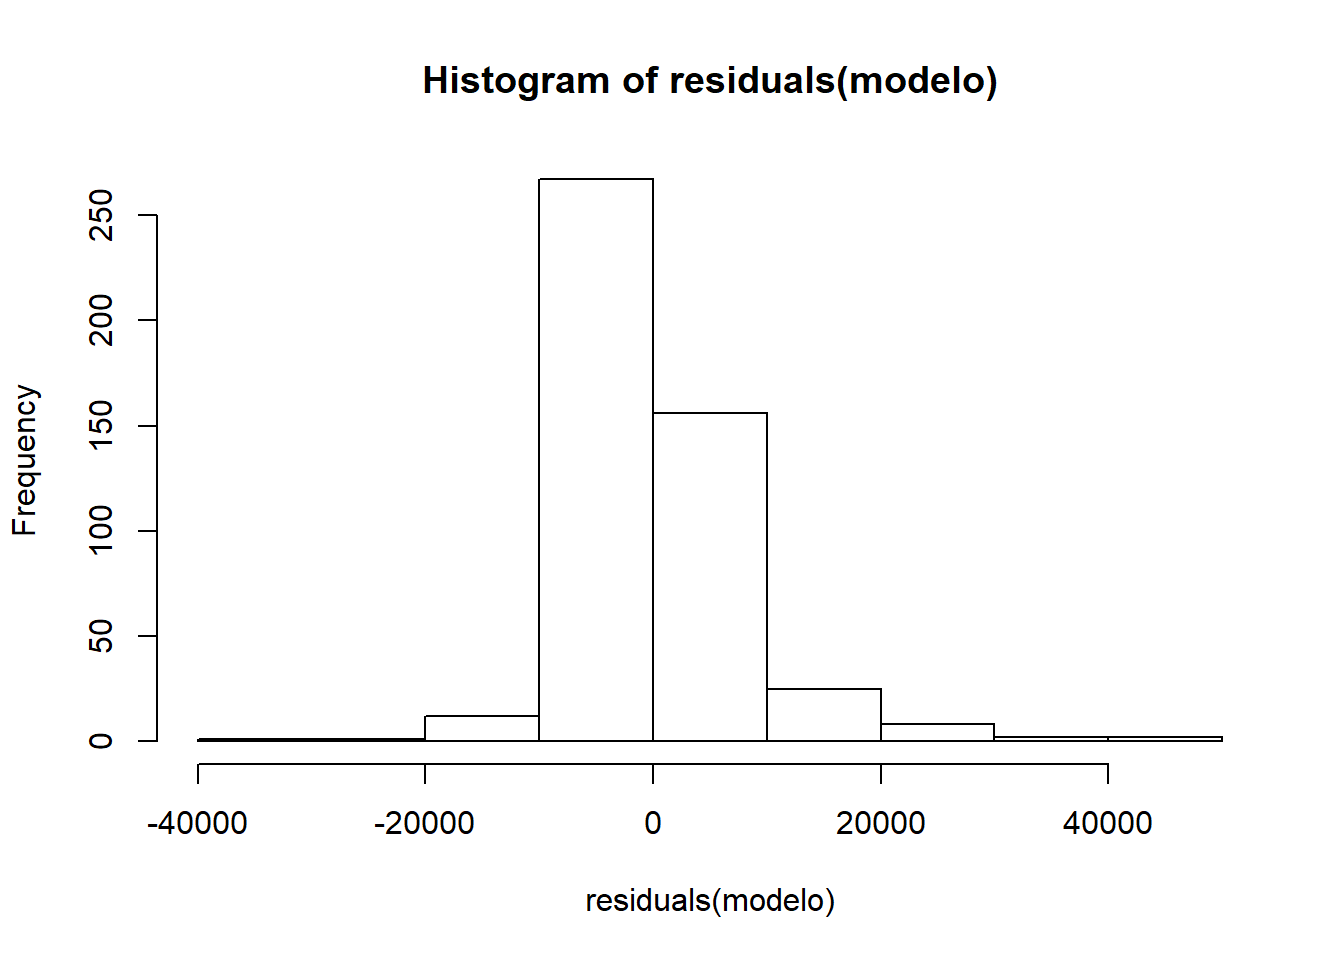
\includegraphics[width=0.7\linewidth]{05-AnalisisExploratorio_files/figure-latex/unnamed-chunk-30-1} \end{center}

\subsection{Diagrama de cajas}\label{diagrama-de-cajas}

Se trata de un gráfico muy polivalente

\begin{Shaded}
\begin{Highlighting}[]
\KeywordTok{boxplot}\NormalTok{(salario, }\DataTypeTok{horizontal=}\NormalTok{T, }\DataTypeTok{axes=}\NormalTok{F)}
\KeywordTok{axis}\NormalTok{(}\DecValTok{1}\NormalTok{)}
\end{Highlighting}
\end{Shaded}

\begin{center}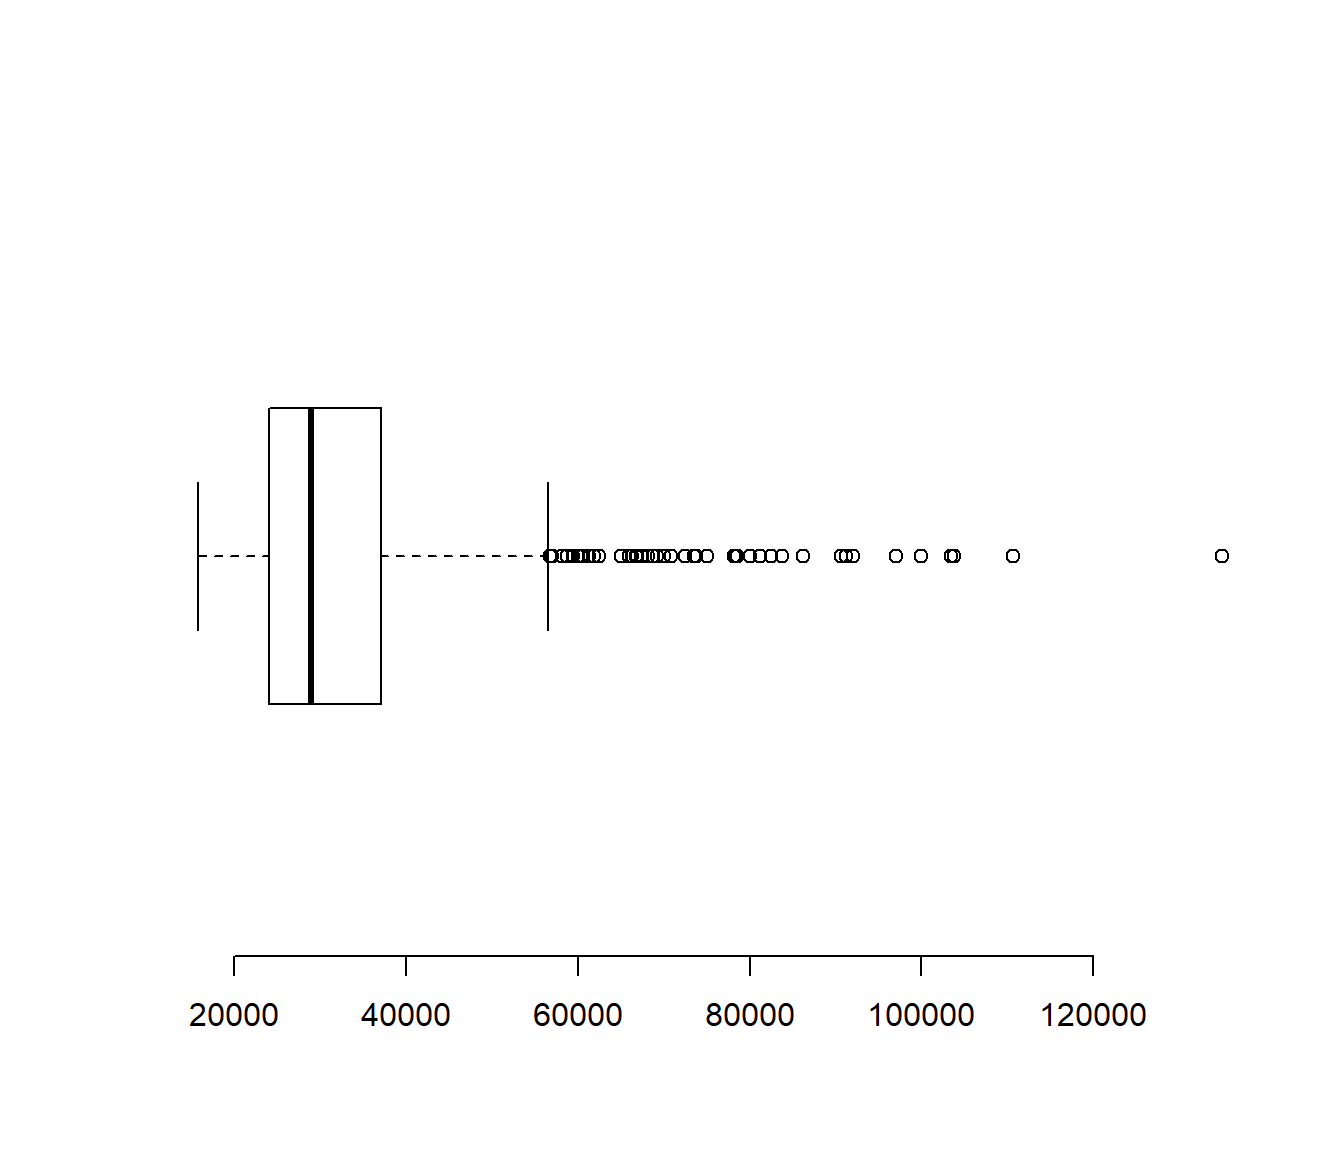
\includegraphics[width=0.7\linewidth]{05-AnalisisExploratorio_files/figure-latex/unnamed-chunk-31-1} \end{center}

\begin{Shaded}
\begin{Highlighting}[]
\KeywordTok{par}\NormalTok{(}\DataTypeTok{mfrow=}\KeywordTok{c}\NormalTok{(}\DecValTok{1}\NormalTok{,}\DecValTok{2}\NormalTok{))}
\KeywordTok{boxplot}\NormalTok{(salario}\OperatorTok{~}\NormalTok{catlab)}
\KeywordTok{boxplot}\NormalTok{(salario}\OperatorTok{~}\NormalTok{sexo)}
\end{Highlighting}
\end{Shaded}

\begin{center}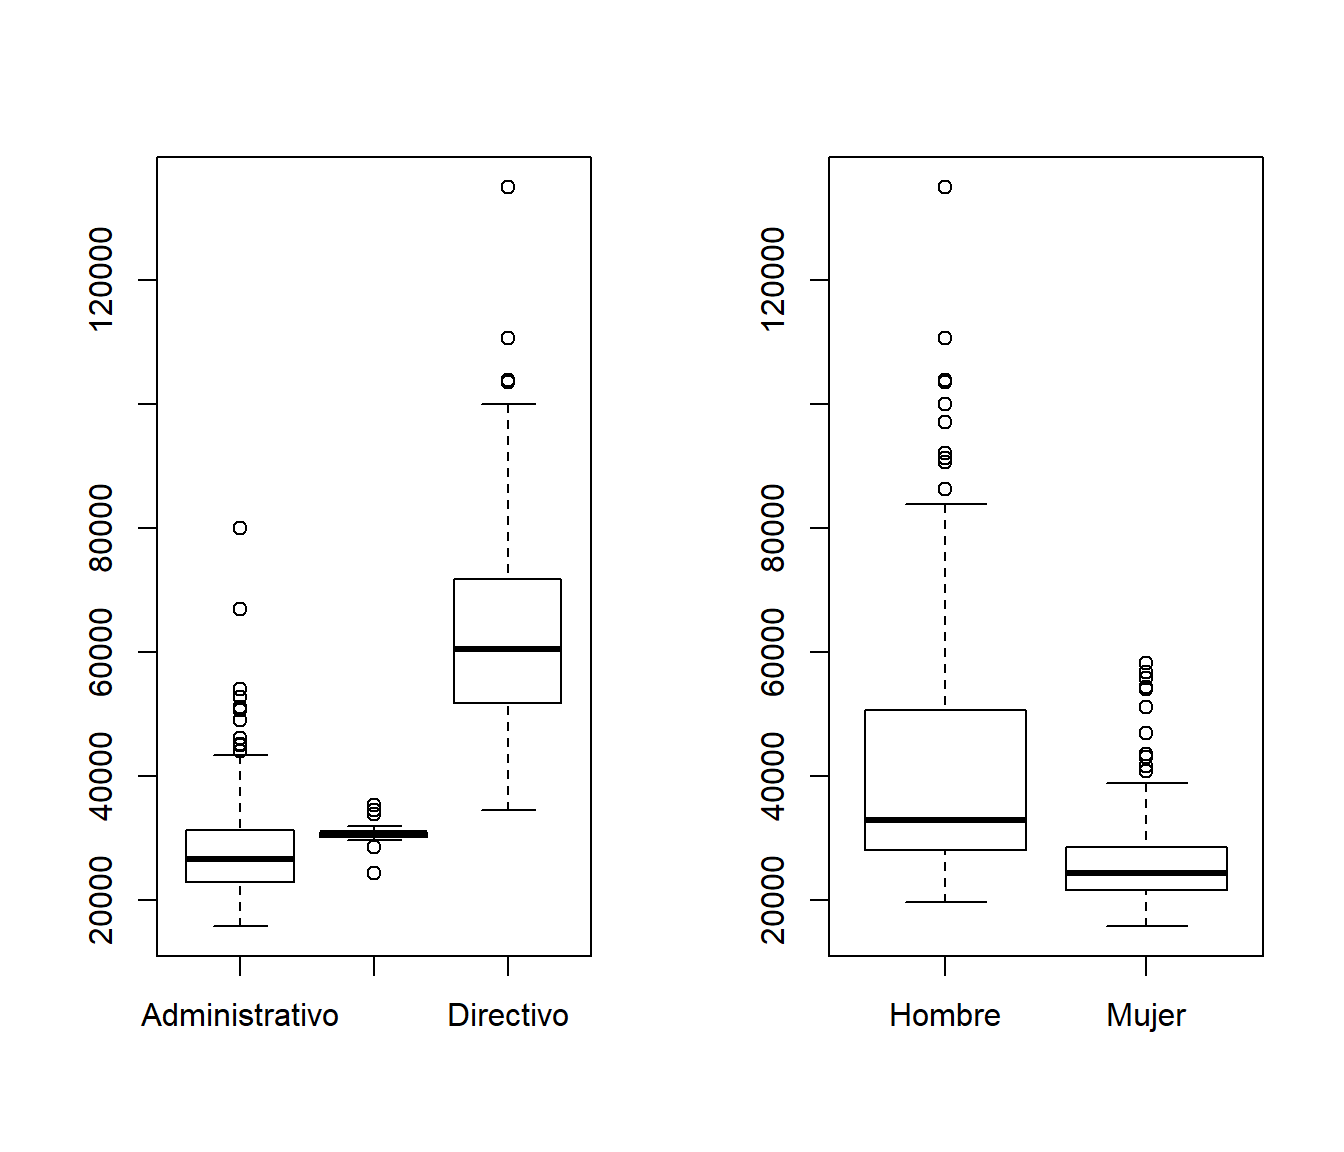
\includegraphics[width=0.7\linewidth]{05-AnalisisExploratorio_files/figure-latex/unnamed-chunk-31-2} \end{center}

\begin{Shaded}
\begin{Highlighting}[]
\KeywordTok{par}\NormalTok{(}\DataTypeTok{mfrow=}\KeywordTok{c}\NormalTok{(}\DecValTok{1}\NormalTok{,}\DecValTok{1}\NormalTok{))}
\KeywordTok{boxplot}\NormalTok{(salario}\OperatorTok{~}\NormalTok{sexo}\OperatorTok{*}\NormalTok{catlab)}
\end{Highlighting}
\end{Shaded}

\begin{center}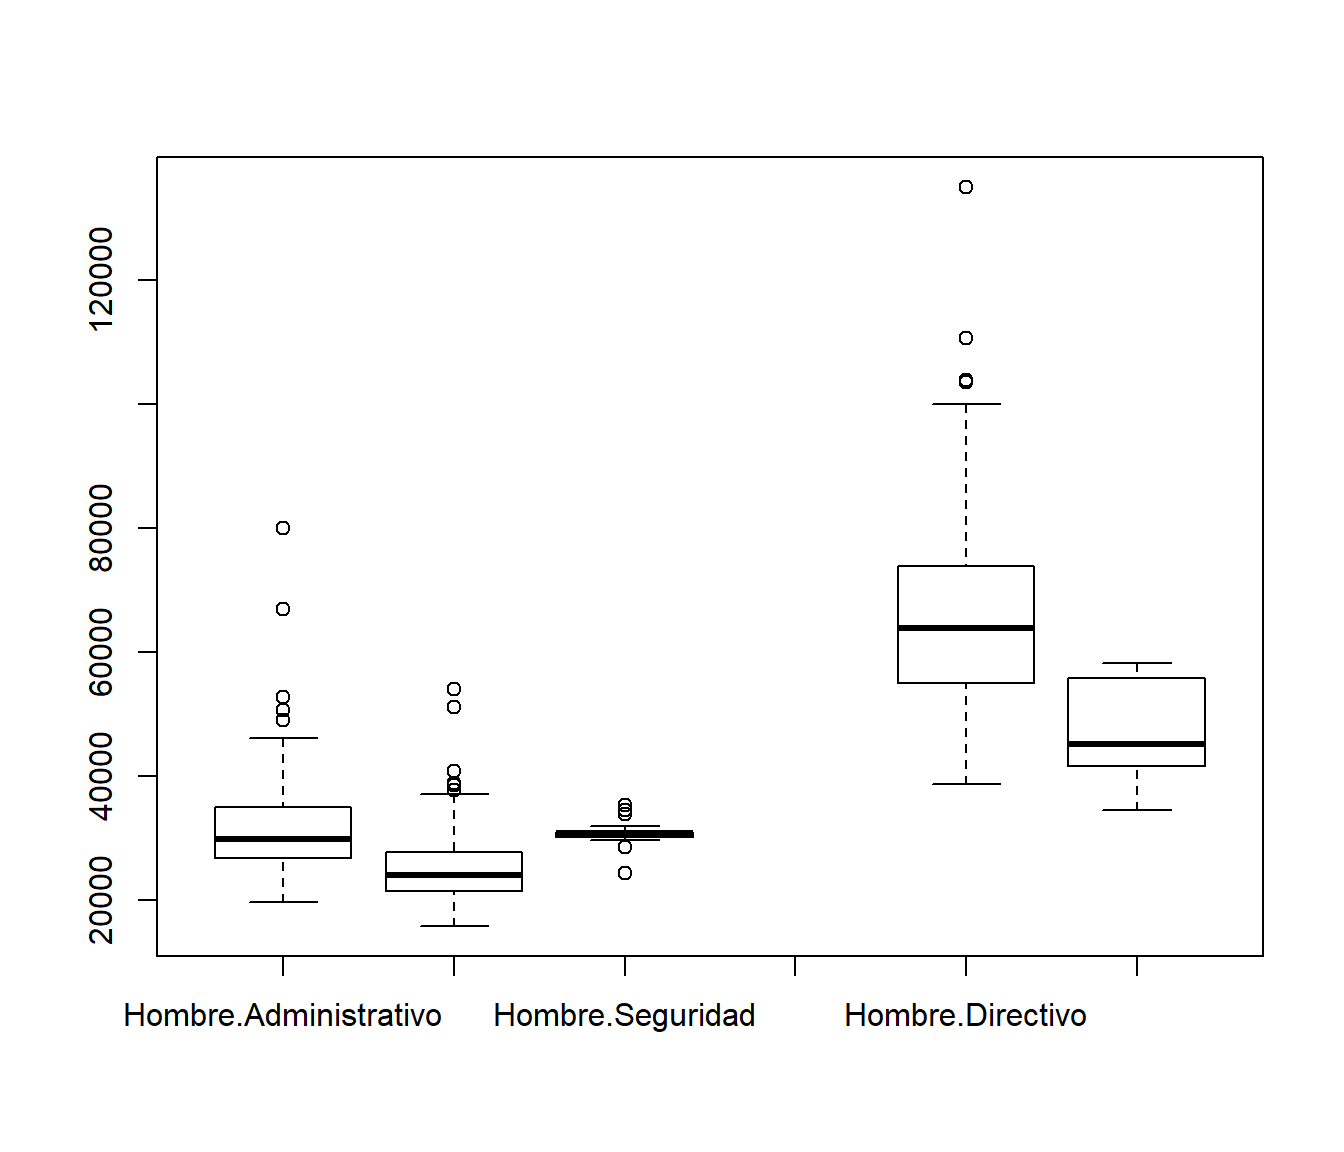
\includegraphics[width=0.7\linewidth]{05-AnalisisExploratorio_files/figure-latex/unnamed-chunk-31-3} \end{center}

\begin{Shaded}
\begin{Highlighting}[]
\KeywordTok{boxplot}\NormalTok{(salini, salario)}
\end{Highlighting}
\end{Shaded}

\begin{center}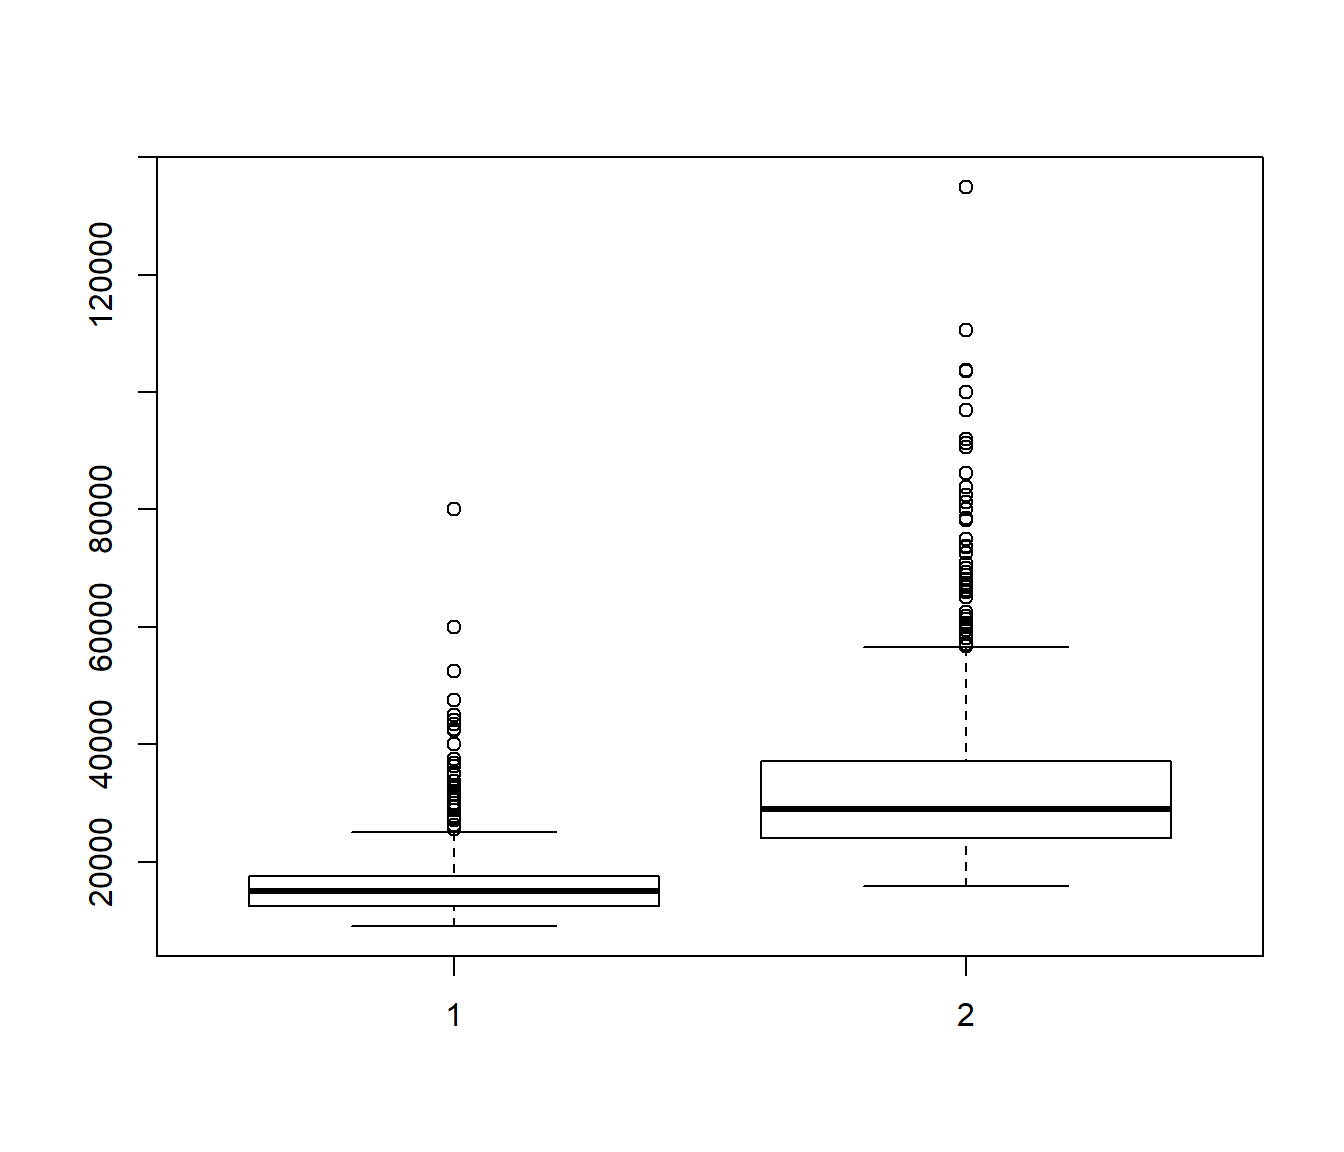
\includegraphics[width=0.7\linewidth]{05-AnalisisExploratorio_files/figure-latex/unnamed-chunk-31-4} \end{center}

\begin{Shaded}
\begin{Highlighting}[]
\KeywordTok{hist}\NormalTok{(salario,}\DataTypeTok{probability=}\NormalTok{T,}\DataTypeTok{ylab=}\StringTok{""}\NormalTok{,}\DataTypeTok{col=}\StringTok{'grey'}\NormalTok{,}\DataTypeTok{axes=}\NormalTok{F,}\DataTypeTok{main=}\StringTok{""}\NormalTok{); }\KeywordTok{axis}\NormalTok{(}\DecValTok{1}\NormalTok{)}
\KeywordTok{lines}\NormalTok{(}\KeywordTok{density}\NormalTok{(salario),}\DataTypeTok{col=}\StringTok{'red'}\NormalTok{,}\DataTypeTok{lwd=}\DecValTok{2}\NormalTok{)}
\KeywordTok{par}\NormalTok{(}\DataTypeTok{new=}\NormalTok{T)}
\KeywordTok{boxplot}\NormalTok{(salario,}\DataTypeTok{horizontal=}\NormalTok{T,}\DataTypeTok{axes=}\NormalTok{F,}\DataTypeTok{lwd=}\DecValTok{2}\NormalTok{)}
\end{Highlighting}
\end{Shaded}

\begin{center}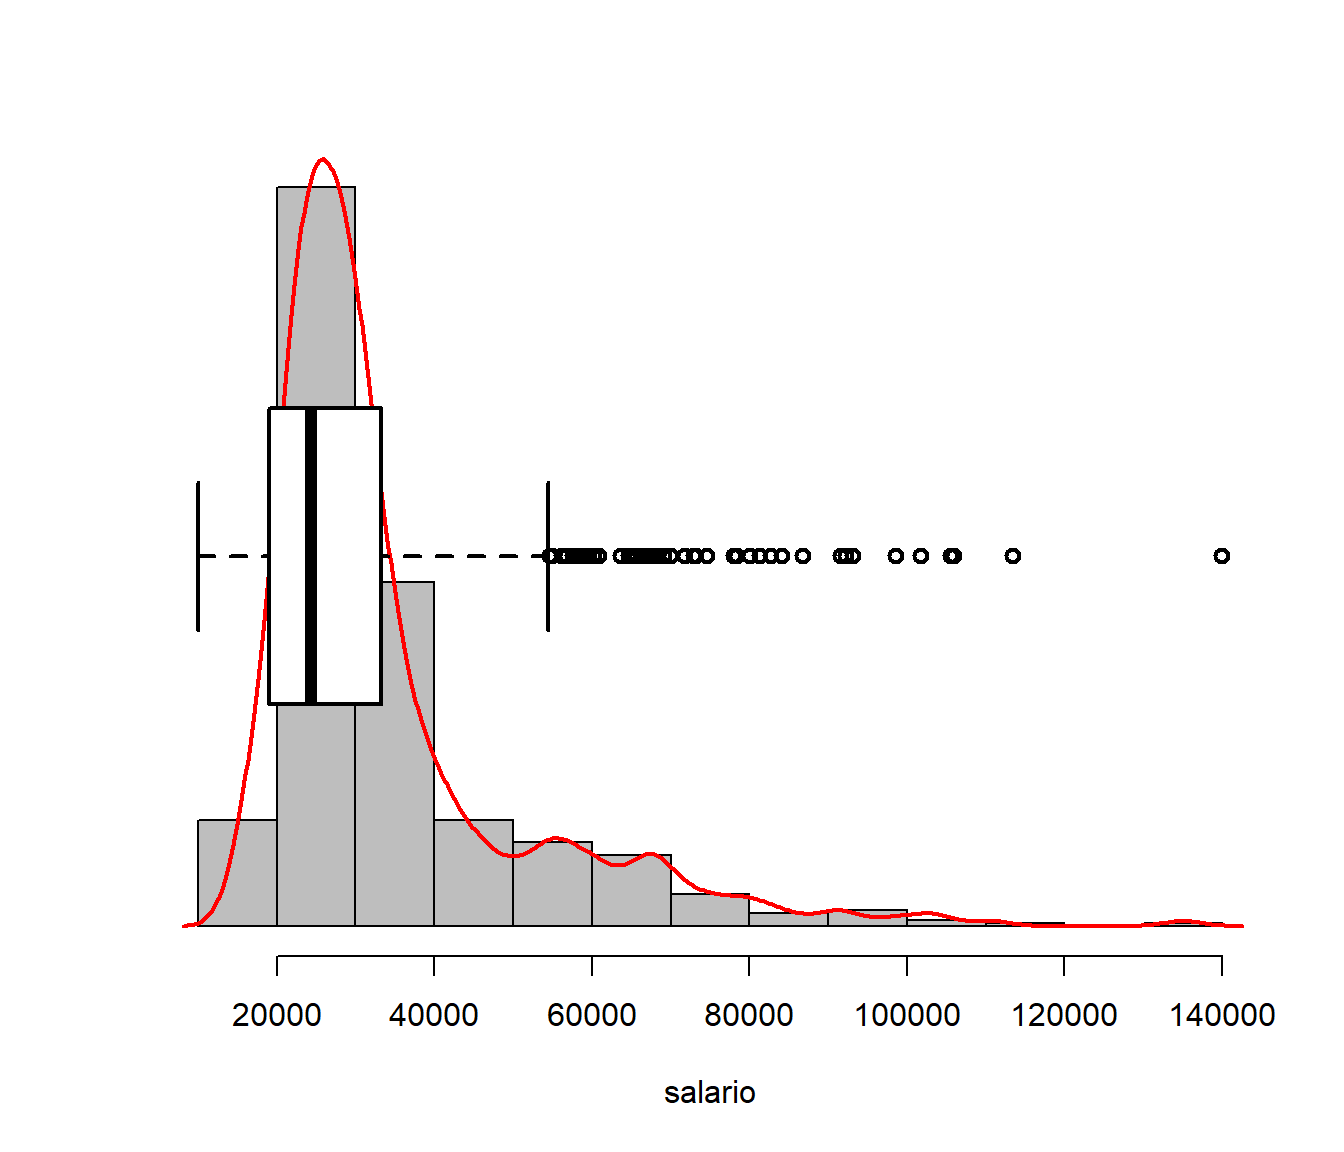
\includegraphics[width=0.7\linewidth]{05-AnalisisExploratorio_files/figure-latex/unnamed-chunk-31-5} \end{center}

\subsection{Gráfica de dispersión}\label{grafica-de-dispersion}

Permite ver la relación entre dos variables:

\begin{Shaded}
\begin{Highlighting}[]
\KeywordTok{plot}\NormalTok{(educ,salario)}
\end{Highlighting}
\end{Shaded}

\begin{center}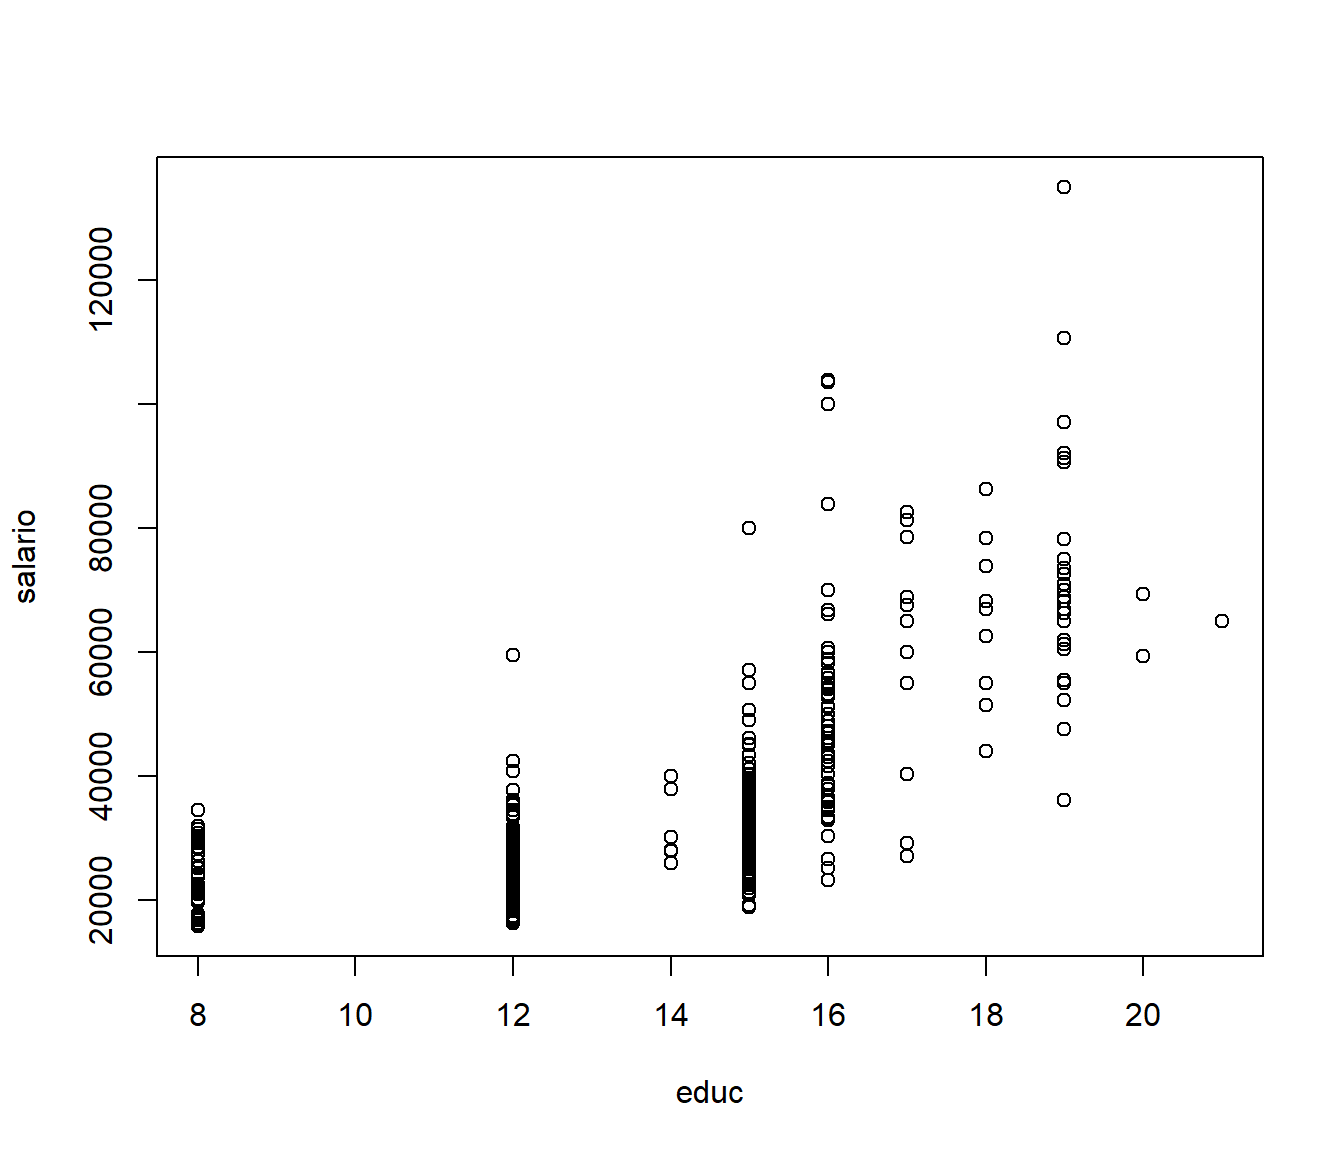
\includegraphics[width=0.7\linewidth]{05-AnalisisExploratorio_files/figure-latex/unnamed-chunk-32-1} \end{center}

\begin{Shaded}
\begin{Highlighting}[]
\KeywordTok{plot}\NormalTok{(tiempemp,salario)}
\end{Highlighting}
\end{Shaded}

\begin{center}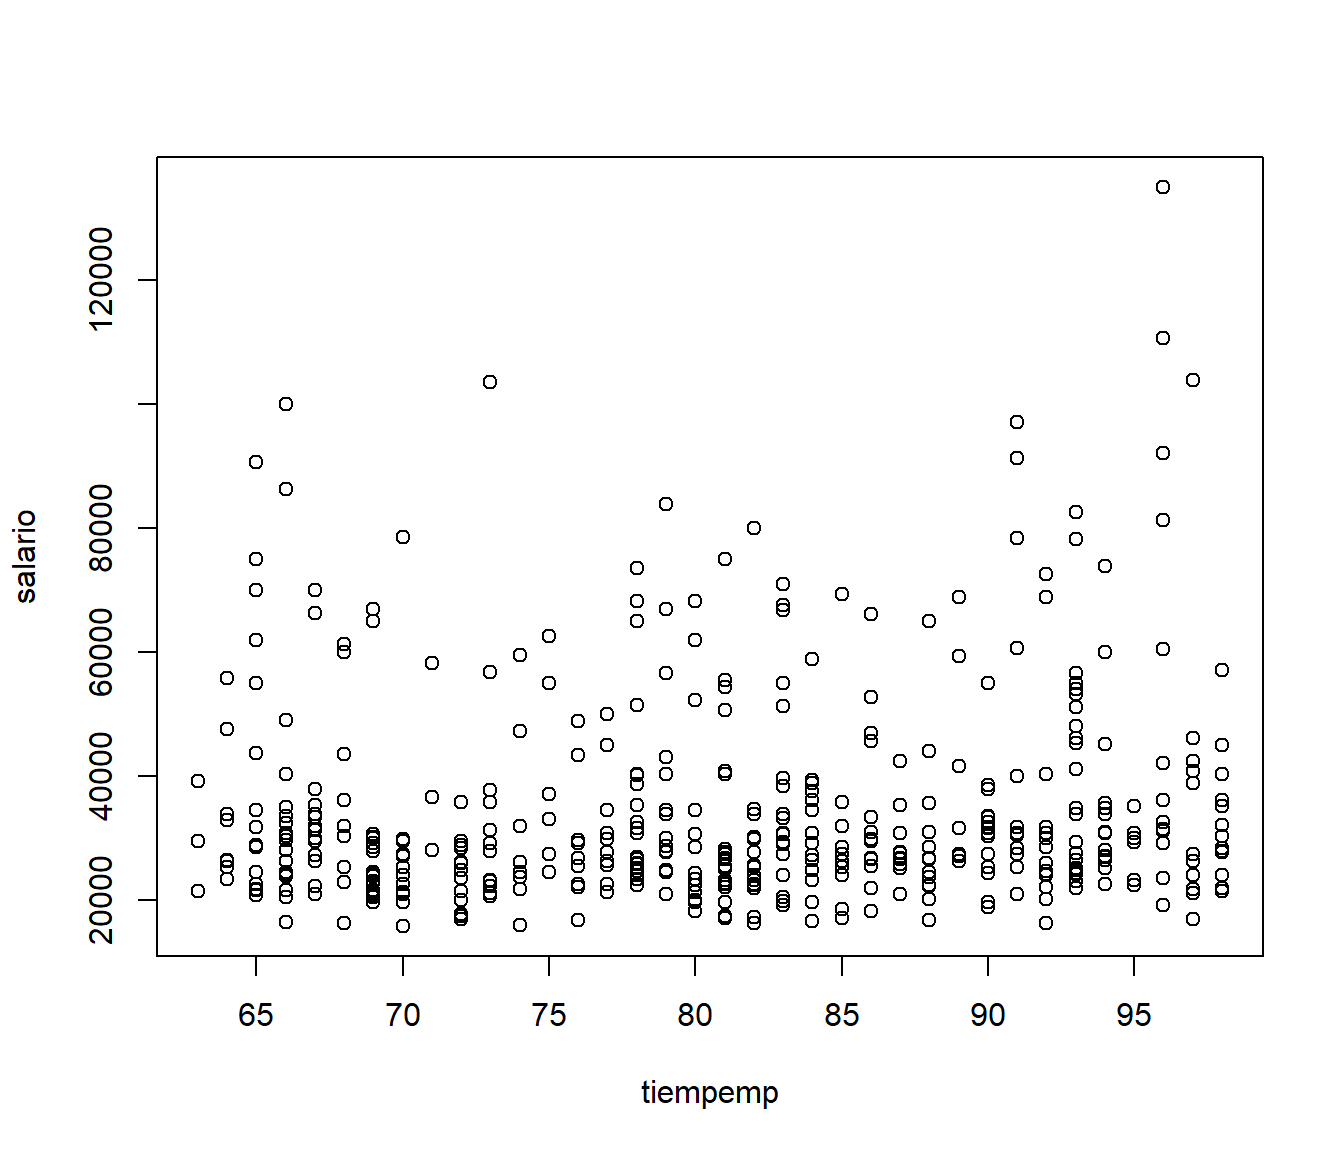
\includegraphics[width=0.7\linewidth]{05-AnalisisExploratorio_files/figure-latex/unnamed-chunk-32-2} \end{center}

\begin{Shaded}
\begin{Highlighting}[]
\KeywordTok{plot}\NormalTok{(salini,salario)}
\end{Highlighting}
\end{Shaded}

\begin{center}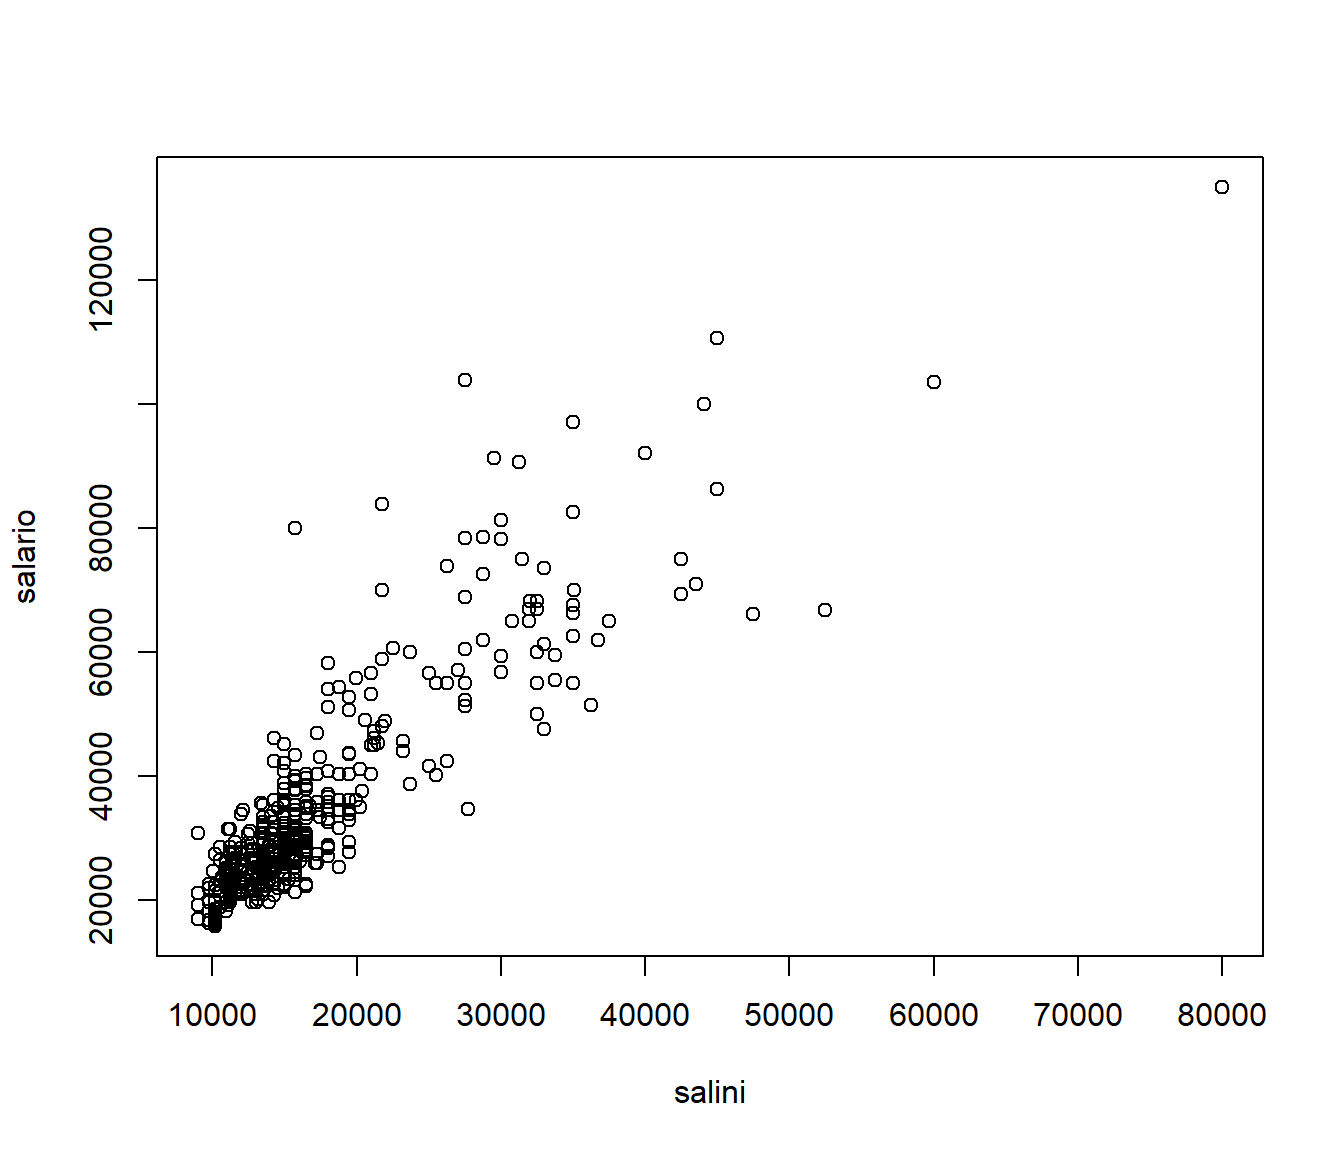
\includegraphics[width=0.7\linewidth]{05-AnalisisExploratorio_files/figure-latex/unnamed-chunk-32-3} \end{center}

En el caso de una serie temporal

\begin{Shaded}
\begin{Highlighting}[]
\NormalTok{AirPassengers}
\end{Highlighting}
\end{Shaded}

\begin{verbatim}
##      Jan Feb Mar Apr May Jun Jul Aug Sep Oct Nov Dec
## 1949 112 118 132 129 121 135 148 148 136 119 104 118
## 1950 115 126 141 135 125 149 170 170 158 133 114 140
## 1951 145 150 178 163 172 178 199 199 184 162 146 166
## 1952 171 180 193 181 183 218 230 242 209 191 172 194
## 1953 196 196 236 235 229 243 264 272 237 211 180 201
## 1954 204 188 235 227 234 264 302 293 259 229 203 229
## 1955 242 233 267 269 270 315 364 347 312 274 237 278
## 1956 284 277 317 313 318 374 413 405 355 306 271 306
## 1957 315 301 356 348 355 422 465 467 404 347 305 336
## 1958 340 318 362 348 363 435 491 505 404 359 310 337
## 1959 360 342 406 396 420 472 548 559 463 407 362 405
## 1960 417 391 419 461 472 535 622 606 508 461 390 432
\end{verbatim}

\begin{Shaded}
\begin{Highlighting}[]
\KeywordTok{plot}\NormalTok{(AirPassengers)}
\end{Highlighting}
\end{Shaded}

\begin{center}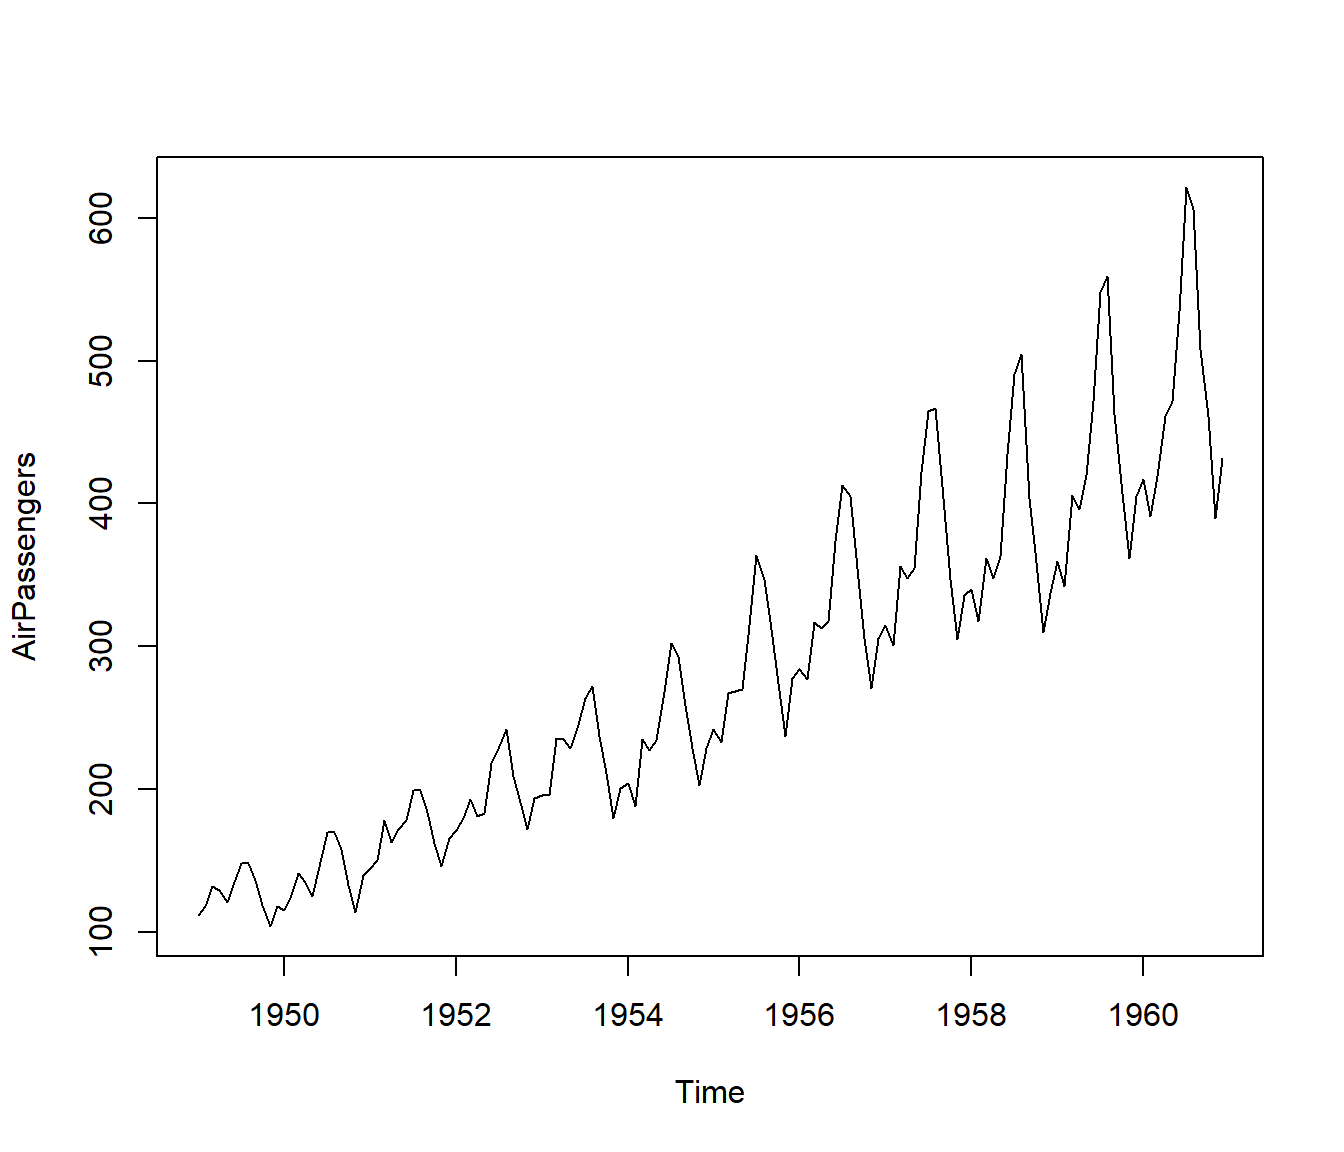
\includegraphics[width=0.7\linewidth]{05-AnalisisExploratorio_files/figure-latex/unnamed-chunk-33-1} \end{center}

Y un último ejemplo utilizando los datos \emph{iris} de Fisher:

\begin{Shaded}
\begin{Highlighting}[]
\KeywordTok{plot}\NormalTok{(iris[,}\DecValTok{3}\NormalTok{],iris[,}\DecValTok{4}\NormalTok{],}\DataTypeTok{main=}\StringTok{"Longitud y anchura de pétalos de lirios"}\NormalTok{,}
     \DataTypeTok{xlab=}\StringTok{"Longitud de pétalo"}\NormalTok{,}\DataTypeTok{ylab=}\StringTok{"Anchura de pétalo"}\NormalTok{)}
\end{Highlighting}
\end{Shaded}

\begin{center}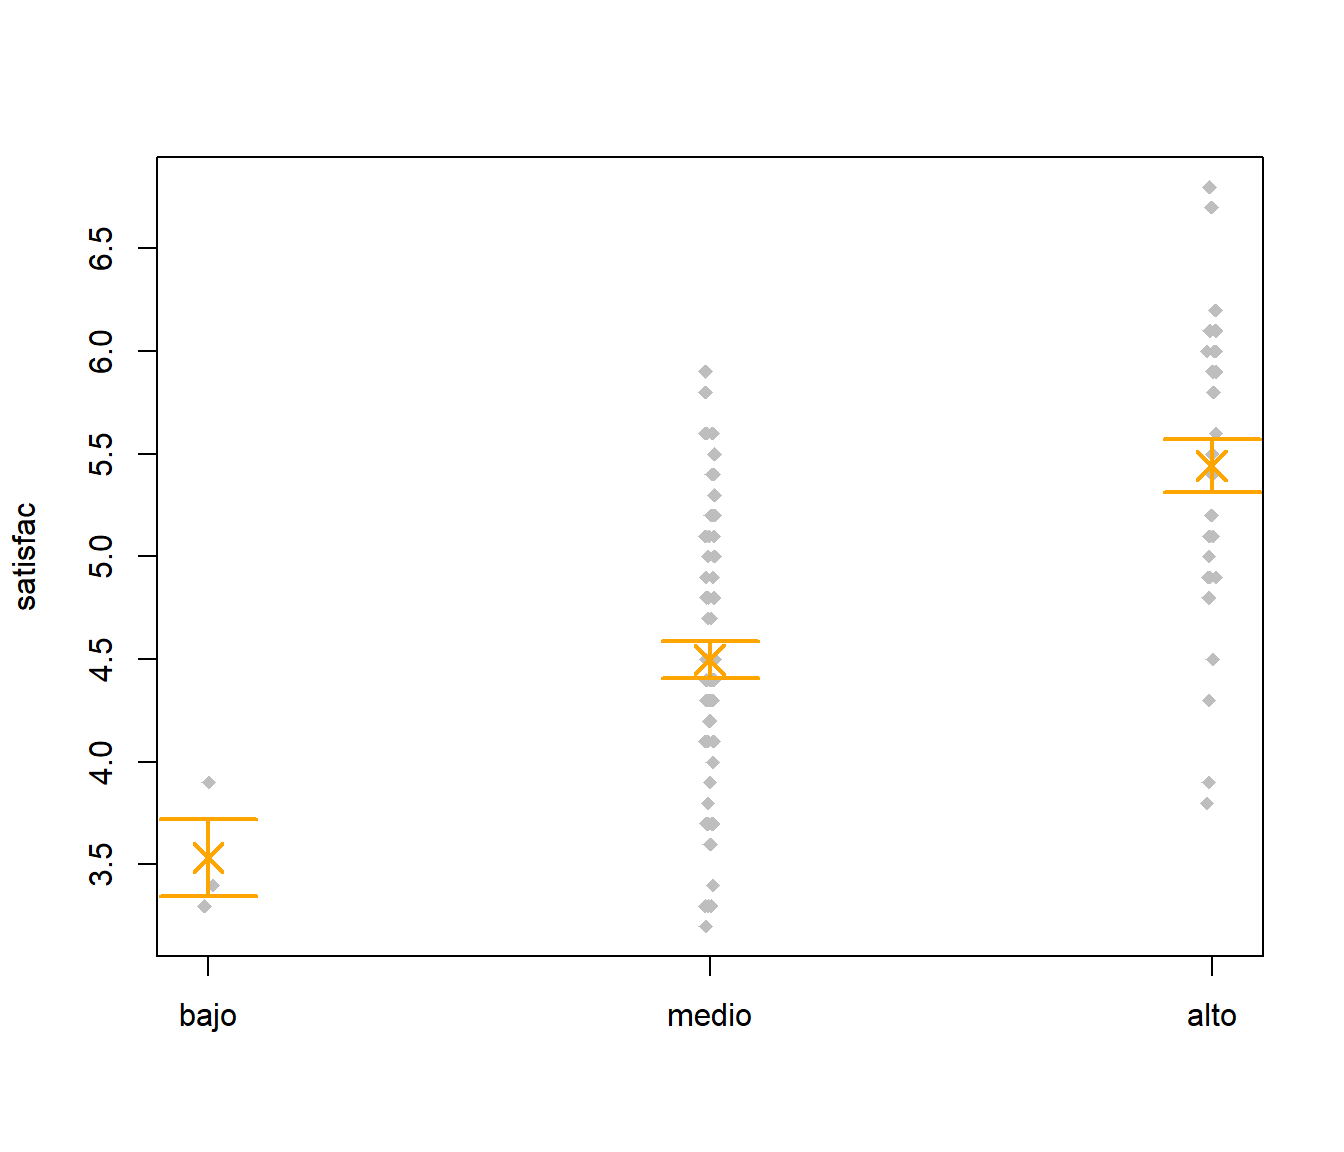
\includegraphics[width=0.7\linewidth]{05-AnalisisExploratorio_files/figure-latex/unnamed-chunk-34-1} \end{center}

\begin{Shaded}
\begin{Highlighting}[]
\NormalTok{iris.color<-}\KeywordTok{c}\NormalTok{(}\StringTok{"red"}\NormalTok{,}\StringTok{"green"}\NormalTok{,}\StringTok{"blue"}\NormalTok{)[iris}\OperatorTok{$}\NormalTok{Species]}
\KeywordTok{plot}\NormalTok{(iris[,}\DecValTok{3}\NormalTok{],iris[,}\DecValTok{4}\NormalTok{],}\DataTypeTok{col=}\NormalTok{iris.color,}\DataTypeTok{main=}\StringTok{"Longitud y anchura}
\StringTok{     de pétalo según especies"}\NormalTok{,}\DataTypeTok{xlab=}\StringTok{"Longitud de pétalo"}\NormalTok{,}
     \DataTypeTok{ylab=}\StringTok{"Anchura de pétalo"}\NormalTok{)}
\KeywordTok{legend}\NormalTok{(}\StringTok{"topleft"}\NormalTok{,}\KeywordTok{c}\NormalTok{(}\StringTok{"Setosa"}\NormalTok{,}\StringTok{"Versicolor"}\NormalTok{,}\StringTok{"Virginica"}\NormalTok{),}\DataTypeTok{pch=}\DecValTok{1}\NormalTok{,}
       \DataTypeTok{col=}\KeywordTok{c}\NormalTok{(}\StringTok{"red"}\NormalTok{,}\StringTok{"green"}\NormalTok{,}\StringTok{"blue"}\NormalTok{),}\DataTypeTok{box.lty=}\DecValTok{0}\NormalTok{)}
\end{Highlighting}
\end{Shaded}

\begin{center}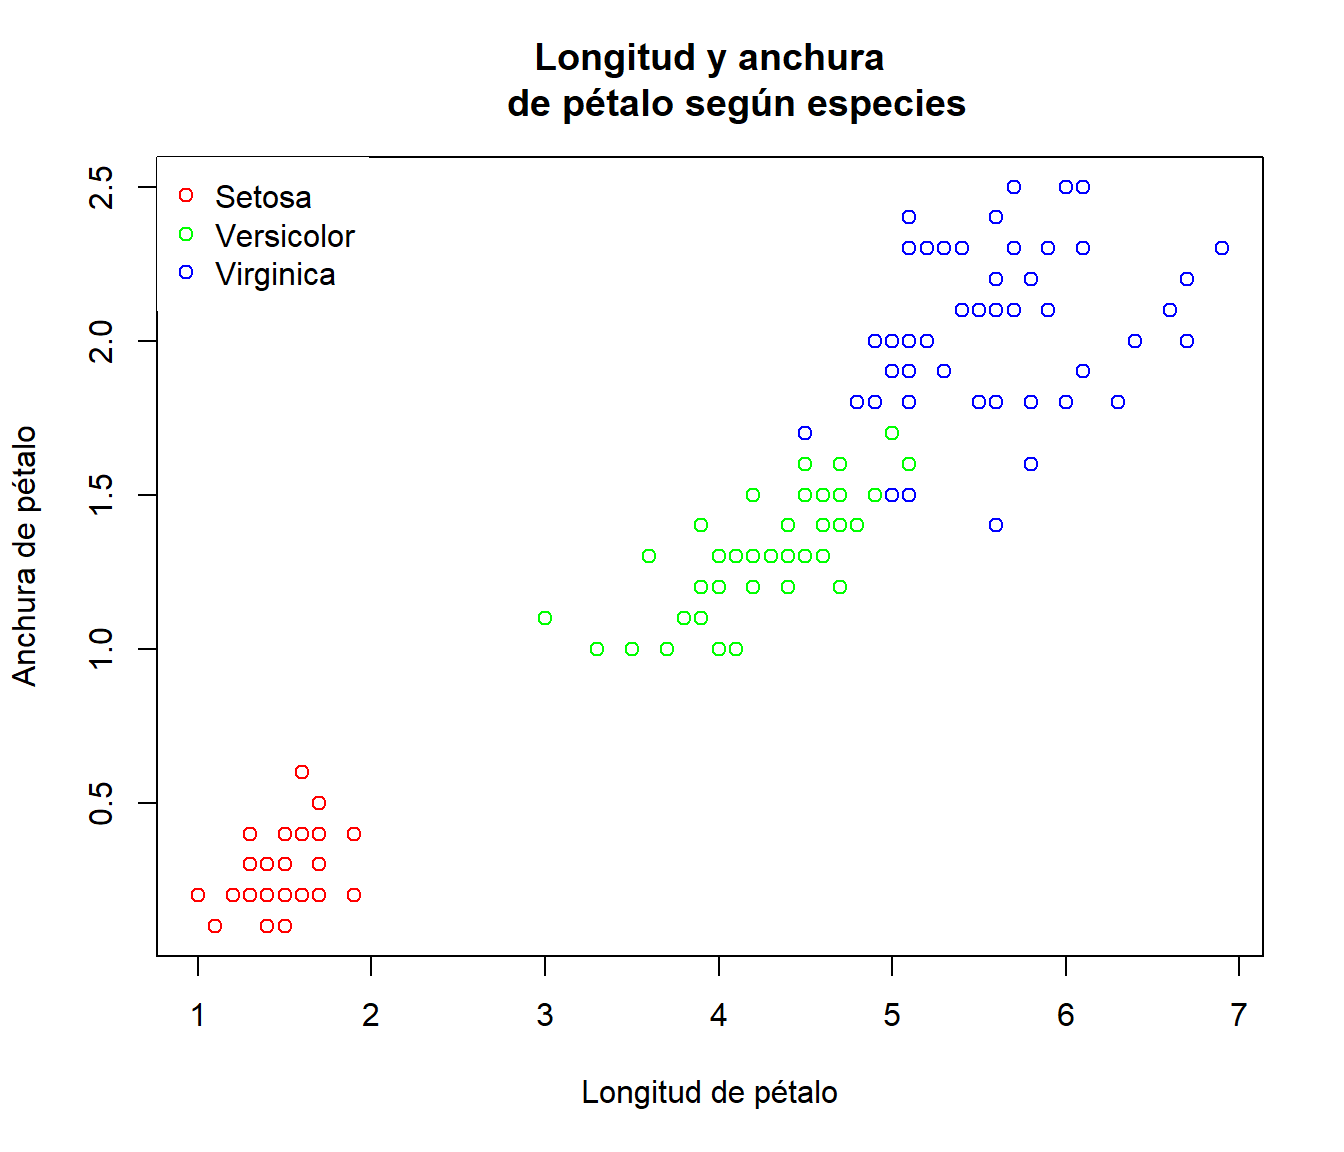
\includegraphics[width=0.7\linewidth]{05-AnalisisExploratorio_files/figure-latex/unnamed-chunk-34-2} \end{center}

\begin{Shaded}
\begin{Highlighting}[]
\KeywordTok{pairs}\NormalTok{(iris[,}\DecValTok{1}\OperatorTok{:}\DecValTok{4}\NormalTok{],}\DataTypeTok{col=}\NormalTok{iris.color)}
\end{Highlighting}
\end{Shaded}

\begin{center}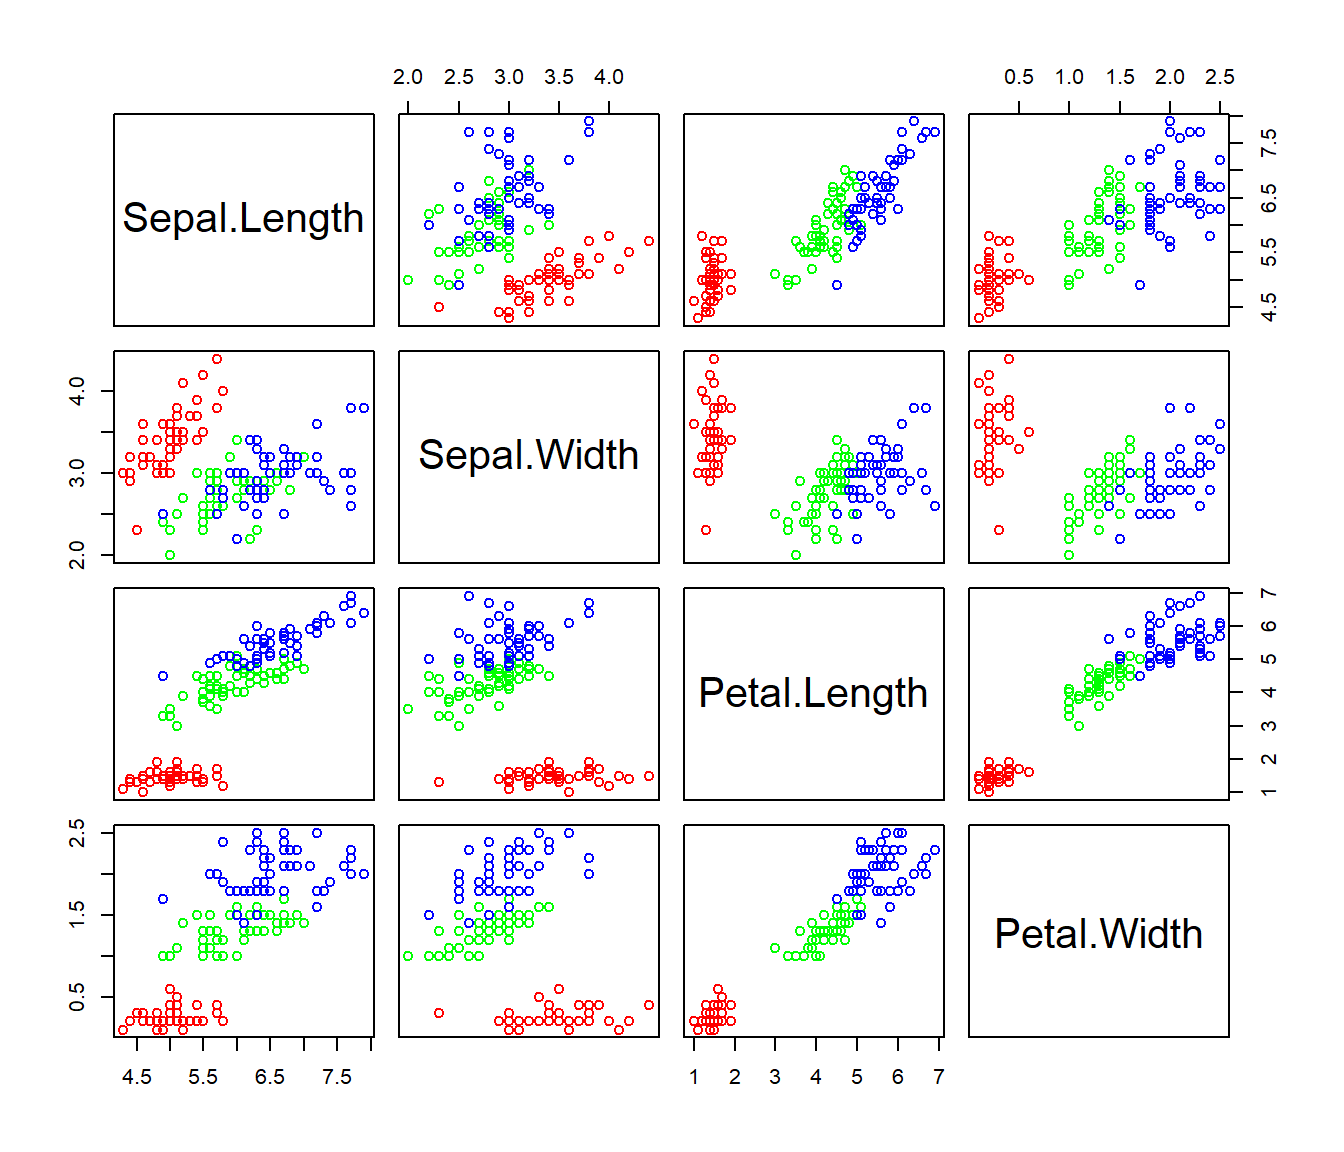
\includegraphics[width=0.7\linewidth]{05-AnalisisExploratorio_files/figure-latex/unnamed-chunk-34-3} \end{center}

\chapter{Modelado de datos}\label{modelado-de-datos}

La realidad puede ser muy compleja por lo que es habitual emplear un
modelo para tratar de explicarla.

\begin{itemize}
\item
  Modelos estocásticos (con componente aleatoria).

  \begin{itemize}
  \item
    Tienen en cuenta la incertidumbre debida a no disponer de la
    suficiente información sobre las variables que influyen en el
    fenómeno en estudio.
  \item
    La inferencia estadística proporciona herramientas para ajustar y
    contrastar la validez del modelo a partir de los datos observados.
  \end{itemize}
\end{itemize}

Sin embargo resultaría muy extraño que la realidad coincida exactamente
con un modelo concreto.

\begin{itemize}
\item
  \href{https://en.wikipedia.org/wiki/George_E._P._Box}{George Box}
  afirmó en su famoso aforismo:

  \begin{quote}
  En esencia, todos los modelos son falsos, pero algunos son útiles.
  \end{quote}
\item
  El objetivo de un modelo es disponer de una aproximación simple de la
  realidad que sea útil.
\end{itemize}

\section{Modelos de regresión}\label{modelos-de-regresion}

Nos centraremos en los modelos de regresión:

\[Y=f(X_{1},\cdots,X_{p})+\varepsilon\] donde:

\begin{itemize}
\item
  \(Y\equiv\) \textbf{variable respuesta} (o dependiente).
\item
  \(\left( X_{1},\cdots,X_{p}\right) \equiv\) \textbf{variables
  explicativas} (independientes, o covariables).
\item
  \(\varepsilon\equiv\) \textbf{error aleatorio.}
\end{itemize}

\subsection{\texorpdfstring{Herramientas disponibles en
\texttt{R}}{Herramientas disponibles en R}}\label{herramientas-disponibles-en-r}

\texttt{R} dispone de múltiples herramientas para trabajar con modelos
de este tipo. Algunas de las funciones y paquetes disponibles se
muestran a continuación:

\begin{itemize}
\item
  Modelos paramétricos:

  \begin{itemize}
  \item
    Modelos lineales:

    \begin{itemize}
    \item
      Regresión lineal: \texttt{lm()} (\texttt{aov()}, \texttt{lme()},
      \texttt{biglm}, \ldots{}).
    \item
      Regresión lineal robusta: \texttt{MASS::rlm()}.
    \item
      Métodos de regularización (Ridge regression, Lasso):
      \texttt{glmnet}, \ldots{}
    \end{itemize}
  \item
    Modelos lineales generalizados: \texttt{glm()} (\texttt{bigglm},
    \ldots{}).
  \item
    Modelos paramétricos no lineales: \texttt{nls()} (\texttt{nlme},
    \ldots{}).
  \end{itemize}
\item
  Modelos no paramétricos:

  \begin{itemize}
  \item
    Regresión local (métodos de suavizado): \texttt{loess()},
    \texttt{KernSmooth}, \texttt{sm}, \ldots{}
  \item
    Modelos aditivos generalizados (GAM): \texttt{gam}, \texttt{mgcv},
    \ldots{}
  \item
    Arboles de decisión (Random Forest, Boosting): \texttt{rpart},
    \texttt{randomForest}, \texttt{xgboost}, \ldots{}
  \item
    Redes neuronales, \ldots{}
  \end{itemize}
\end{itemize}

Desde el punto de vista de la programación, con todos estos modelos se
trabaja de una forma muy similar en \texttt{R}.

\section{Fórmulas}\label{formulas}

En \texttt{R} para especificar un modelo estadístico (realmente una
familia) se suelen emplear fórmulas (también para generar gráficos). Son
de la forma:

\begin{Shaded}
\begin{Highlighting}[]
\NormalTok{respuesta }\OperatorTok{~}\StringTok{ }\NormalTok{modelo}
\end{Highlighting}
\end{Shaded}

\texttt{modelo} especifica los ``términos'' mediante operadores (tienen
un significado especial en este contexto):

\begin{longtable}[]{@{}ll@{}}
\toprule
Operador & Descripción\tabularnewline
\midrule
\endhead
\texttt{a+b} & incluye \texttt{a} y \texttt{b} (efectos
principales)\tabularnewline
\texttt{-b} & excluye \texttt{b} del modelo\tabularnewline
\texttt{a:b} & interacción de \texttt{a} y \texttt{b}\tabularnewline
\ & \texttt{b\ \%in\%\ a} efectos de \texttt{b} anidados en \texttt{a}
(\texttt{a:b})\tabularnewline
\ & \texttt{a/b\ =\ a\ +\ b\ \%in\%\ a\ =\ a\ +\ a:b}\tabularnewline
\texttt{a*b\ =\ a+b+a:b} & efectos principales más
interacciones\tabularnewline
\texttt{\^{}n} & interacciones hasta nivel \texttt{n}
(\texttt{(a+b)\^{}2\ =\ a+b+a:b})\tabularnewline
\texttt{poly(a,\ n)} & polinomios de \texttt{a} hasta grado
\texttt{n}\tabularnewline
\texttt{1} & término constante\tabularnewline
\texttt{.} & todas las variables disponibles o modelo actual en
actualizaciones\tabularnewline
\bottomrule
\end{longtable}

Para realizar operaciones aritméticas (que incluyan \texttt{+},
\texttt{-}, \texttt{*}, \texttt{\^{}}, \texttt{1}, \ldots{}) es
necesario ``aislar'' la operación dentro una función (e.g.
\texttt{log(abs(x)\ +\ 1)}). Por ejemplo, para realizar un ajuste
cuadrático se debería utilizar
\texttt{y\ \textasciitilde{}\ x\ +\ I(x\^{}2)}, ya que
\texttt{y\ \textasciitilde{}\ x\ +\ x\^{}2\ =\ y\ \textasciitilde{}\ x}
(la interacción \texttt{x:x\ =\ x}).

\begin{itemize}
\tightlist
\item
  \texttt{I()} función identidad.
\end{itemize}

\section{Ejemplo: regresión lineal
simple}\label{ejemplo-regresion-lineal-simple}

Introducido en descriptiva y con referencias al tema siguiente

\chapter{Modelos lineales}\label{modelos-lineales}

Suponen que la función de regresión es lineal:

\[Y=\beta_{0}+\beta_{1}X_{1}+\beta_{2}X_{2}+\cdots+\beta_{p}X_{p}+\varepsilon\]

El efecto de las variables explicativas sobre la respuesta es simple
(proporcional a su valor).

\section{Ejemplo}\label{ejemplo}

El fichero \emph{hatco.RData} contiene observaciones de clientes de la
compañía de distribución industrial (Compañía Hair, Anderson y Tatham).
Las variables se pueden clasificar en tres grupos:

\begin{Shaded}
\begin{Highlighting}[]
\KeywordTok{load}\NormalTok{(}\StringTok{'datos/hatco.RData'}\NormalTok{)}
\KeywordTok{as.data.frame}\NormalTok{(}\KeywordTok{attr}\NormalTok{(hatco, }\StringTok{"variable.labels"}\NormalTok{))}
\end{Highlighting}
\end{Shaded}

\begin{verbatim}
##          attr(hatco, "variable.labels")
## empresa                         Empresa
## tamano             Tamaño de la empresa
## adquisic      Estructura de adquisición
## tindustr              Tipo de industria
## tsitcomp    Tipo de situación de compra
## velocida           Velocidad de entrega
## precio                 Nivel de precios
## flexprec        Flexibilidad de precios
## imgfabri          Imagen del fabricante
## servconj              Servicio conjunto
## imgfvent     Imagen de fuerza de ventas
## calidadp            Calidad de producto
## fidelida   Porcentaje de compra a HATCO
## satisfac            Satisfacción global
## nfidelid        Nivel de compra a HATCO
## nsatisfa          Nivel de satisfacción
\end{verbatim}

Consideraremos como respuesta la variable \emph{fidelida} y como
variables explicativas el resto de variables continuas menos
\emph{satisfac}.

\begin{Shaded}
\begin{Highlighting}[]
\NormalTok{datos <-}\StringTok{ }\NormalTok{hatco[, }\DecValTok{6}\OperatorTok{:}\DecValTok{13}\NormalTok{]  }\CommentTok{# Nota: realmente no copia el objeto...}
\KeywordTok{plot}\NormalTok{(datos)}
\end{Highlighting}
\end{Shaded}

\includegraphics{08-ModelosLineales_files/figure-latex/unnamed-chunk-2-1.pdf}

\begin{Shaded}
\begin{Highlighting}[]
\CommentTok{# cor(datos, use = "complete") # Por defecto 8 decimales...}
\KeywordTok{print}\NormalTok{(}\KeywordTok{cor}\NormalTok{(datos, }\DataTypeTok{use =} \StringTok{"complete"}\NormalTok{), }\DataTypeTok{digits =} \DecValTok{2}\NormalTok{)}
\end{Highlighting}
\end{Shaded}

\begin{verbatim}
##          velocida precio flexprec imgfabri servconj imgfvent calidadp
## velocida    1.000 -0.354    0.519    0.049    0.609    0.081   -0.490
## precio     -0.354  1.000   -0.486    0.272    0.511    0.189    0.468
## flexprec    0.519 -0.486    1.000   -0.115    0.075   -0.038   -0.445
## imgfabri    0.049  0.272   -0.115    1.000    0.298    0.790    0.199
## servconj    0.609  0.511    0.075    0.298    1.000    0.246   -0.062
## imgfvent    0.081  0.189   -0.038    0.790    0.246    1.000    0.181
## calidadp   -0.490  0.468   -0.445    0.199   -0.062    0.181    1.000
## fidelida    0.674  0.077    0.578    0.224    0.698    0.267   -0.204
##          fidelida
## velocida    0.674
## precio      0.077
## flexprec    0.578
## imgfabri    0.224
## servconj    0.698
## imgfvent    0.267
## calidadp   -0.204
## fidelida    1.000
\end{verbatim}

\section{\texorpdfstring{Ajuste: función
\texttt{lm}}{Ajuste: función lm}}\label{ajuste-funcion-lm}

Para el ajuste (estimación de los parámetros) de un modelo lineal a un
conjunto de datos (por mínimos cuadrados) se emplea la función
\texttt{lm}:

\begin{Shaded}
\begin{Highlighting}[]
\NormalTok{ajuste <-}\StringTok{ }\KeywordTok{lm}\NormalTok{(formula, datos, seleccion, pesos, na.action)}
\end{Highlighting}
\end{Shaded}

\begin{itemize}
\tightlist
\item
  \texttt{formula} fórmula que especifica el modelo.
\item
  \texttt{datos} data.frame opcional con las variables de la formula.
\item
  \texttt{seleccion} especificación opcional de un subconjunto de
  observaciones.
\item
  \texttt{pesos} vector opcional de pesos (WLS).
\item
  \texttt{na.action} opción para manejar los datos faltantes
  (\texttt{na.omit}).
\end{itemize}

\begin{Shaded}
\begin{Highlighting}[]
\NormalTok{modelo <-}\StringTok{ }\KeywordTok{lm}\NormalTok{(fidelida }\OperatorTok{~}\StringTok{ }\NormalTok{servconj, datos)}
\NormalTok{modelo}
\end{Highlighting}
\end{Shaded}

\begin{verbatim}
## 
## Call:
## lm(formula = fidelida ~ servconj, data = datos)
## 
## Coefficients:
## (Intercept)     servconj  
##       21.98         8.30
\end{verbatim}

Al imprimir el ajuste resultante se muestra un pequeño resumen del
ajuste (aunque el objeto que contiene los resultados es una lista).

Para obtener un resumen más completo se puede utilizar la función
\texttt{summary()}.

\begin{Shaded}
\begin{Highlighting}[]
\KeywordTok{summary}\NormalTok{(modelo)}
\end{Highlighting}
\end{Shaded}

\begin{verbatim}
## 
## Call:
## lm(formula = fidelida ~ servconj, data = datos)
## 
## Residuals:
##      Min       1Q   Median       3Q      Max 
## -14.1956  -4.0655   0.2944   4.5945  11.9744 
## 
## Coefficients:
##             Estimate Std. Error t value Pr(>|t|)    
## (Intercept)  21.9754     2.6086   8.424 3.34e-13 ***
## servconj      8.3000     0.8645   9.601 9.76e-16 ***
## ---
## Signif. codes:  0 '***' 0.001 '**' 0.01 '*' 0.05 '.' 0.1 ' ' 1
## 
## Residual standard error: 6.432 on 97 degrees of freedom
##   (1 observation deleted due to missingness)
## Multiple R-squared:  0.4872, Adjusted R-squared:  0.482 
## F-statistic: 92.17 on 1 and 97 DF,  p-value: 9.765e-16
\end{verbatim}

\begin{Shaded}
\begin{Highlighting}[]
\KeywordTok{plot}\NormalTok{(fidelida }\OperatorTok{~}\StringTok{ }\NormalTok{servconj, datos)}
\KeywordTok{abline}\NormalTok{(modelo)}
\end{Highlighting}
\end{Shaded}

\includegraphics{08-ModelosLineales_files/figure-latex/unnamed-chunk-7-1.pdf}

\subsection{Extracción de información}\label{extraccion-de-informacion}

Para la extracción de información se pueden acceder a los componentes
del modelo ajustado o emplear funciones (genéricas). Algunas de las más
utilizadas son las siguientes:

\begin{longtable}[]{@{}ll@{}}
\toprule
\begin{minipage}[b]{0.10\columnwidth}\raggedright\strut
Función\strut
\end{minipage} & \begin{minipage}[b]{0.68\columnwidth}\raggedright\strut
Descripción\strut
\end{minipage}\tabularnewline
\midrule
\endhead
\begin{minipage}[t]{0.10\columnwidth}\raggedright\strut
\texttt{fitted}\strut
\end{minipage} & \begin{minipage}[t]{0.68\columnwidth}\raggedright\strut
valores ajustados\strut
\end{minipage}\tabularnewline
\begin{minipage}[t]{0.10\columnwidth}\raggedright\strut
\texttt{coef}\strut
\end{minipage} & \begin{minipage}[t]{0.68\columnwidth}\raggedright\strut
coeficientes estimados (y errores estándar)\strut
\end{minipage}\tabularnewline
\begin{minipage}[t]{0.10\columnwidth}\raggedright\strut
\texttt{confint}\strut
\end{minipage} & \begin{minipage}[t]{0.68\columnwidth}\raggedright\strut
intervalos de confianza para los coeficientes\strut
\end{minipage}\tabularnewline
\begin{minipage}[t]{0.10\columnwidth}\raggedright\strut
\texttt{residuals}\strut
\end{minipage} & \begin{minipage}[t]{0.68\columnwidth}\raggedright\strut
residuos\strut
\end{minipage}\tabularnewline
\begin{minipage}[t]{0.10\columnwidth}\raggedright\strut
\texttt{plot}\strut
\end{minipage} & \begin{minipage}[t]{0.68\columnwidth}\raggedright\strut
gráficos de diagnóstico\strut
\end{minipage}\tabularnewline
\begin{minipage}[t]{0.10\columnwidth}\raggedright\strut
\texttt{termplot}\strut
\end{minipage} & \begin{minipage}[t]{0.68\columnwidth}\raggedright\strut
gráfico de efectos parciales\strut
\end{minipage}\tabularnewline
\begin{minipage}[t]{0.10\columnwidth}\raggedright\strut
\texttt{anova}\strut
\end{minipage} & \begin{minipage}[t]{0.68\columnwidth}\raggedright\strut
calcula tablas de análisis de varianza (también permite comparar
modelos)\strut
\end{minipage}\tabularnewline
\begin{minipage}[t]{0.10\columnwidth}\raggedright\strut
\texttt{predict}\strut
\end{minipage} & \begin{minipage}[t]{0.68\columnwidth}\raggedright\strut
calcula predicciones para nuevos datos\strut
\end{minipage}\tabularnewline
\bottomrule
\end{longtable}

Ejemplo:

\begin{Shaded}
\begin{Highlighting}[]
\NormalTok{modelo2 <-}\StringTok{ }\KeywordTok{lm}\NormalTok{(fidelida }\OperatorTok{~}\StringTok{ }\NormalTok{servconj }\OperatorTok{+}\StringTok{ }\NormalTok{flexprec, }\DataTypeTok{data =}\NormalTok{ hatco)}
\KeywordTok{summary}\NormalTok{(modelo2)}
\end{Highlighting}
\end{Shaded}

\begin{verbatim}
## 
## Call:
## lm(formula = fidelida ~ servconj + flexprec, data = hatco)
## 
## Residuals:
##      Min       1Q   Median       3Q      Max 
## -10.2549  -2.2850   0.3411   3.3260   7.0853 
## 
## Coefficients:
##             Estimate Std. Error t value Pr(>|t|)    
## (Intercept)  -3.4617     2.9734  -1.164    0.247    
## servconj      7.8287     0.5897  13.276   <2e-16 ***
## flexprec      3.4017     0.3191  10.661   <2e-16 ***
## ---
## Signif. codes:  0 '***' 0.001 '**' 0.01 '*' 0.05 '.' 0.1 ' ' 1
## 
## Residual standard error: 4.375 on 96 degrees of freedom
##   (1 observation deleted due to missingness)
## Multiple R-squared:  0.7652, Adjusted R-squared:  0.7603 
## F-statistic: 156.4 on 2 and 96 DF,  p-value: < 2.2e-16
\end{verbatim}

\begin{Shaded}
\begin{Highlighting}[]
\KeywordTok{confint}\NormalTok{(modelo2)}
\end{Highlighting}
\end{Shaded}

\begin{verbatim}
##                 2.5 %   97.5 %
## (Intercept) -9.363813 2.440344
## servconj     6.658219 8.999274
## flexprec     2.768333 4.035030
\end{verbatim}

\begin{Shaded}
\begin{Highlighting}[]
\KeywordTok{anova}\NormalTok{(modelo2)}
\end{Highlighting}
\end{Shaded}

\begin{verbatim}
## Analysis of Variance Table
## 
## Response: fidelida
##           Df Sum Sq Mean Sq F value    Pr(>F)    
## servconj   1 3813.6  3813.6  199.23 < 2.2e-16 ***
## flexprec   1 2175.6  2175.6  113.66 < 2.2e-16 ***
## Residuals 96 1837.6    19.1                      
## ---
## Signif. codes:  0 '***' 0.001 '**' 0.01 '*' 0.05 '.' 0.1 ' ' 1
\end{verbatim}

\begin{Shaded}
\begin{Highlighting}[]
\CommentTok{# anova(modelo2, modelo)}
\CommentTok{# termplot(modelo2, partial.resid = TRUE)}
\end{Highlighting}
\end{Shaded}

Muchas de estas funciones genéricas son válidas para otros tipos de
modelos (glm, \ldots{}).

Algunas funciones como \texttt{summary()} devuelven información
adicional:

\begin{Shaded}
\begin{Highlighting}[]
\NormalTok{res <-}\StringTok{ }\KeywordTok{summary}\NormalTok{(modelo2)}
\KeywordTok{names}\NormalTok{(res)}
\end{Highlighting}
\end{Shaded}

\begin{verbatim}
##  [1] "call"          "terms"         "residuals"     "coefficients" 
##  [5] "aliased"       "sigma"         "df"            "r.squared"    
##  [9] "adj.r.squared" "fstatistic"    "cov.unscaled"  "na.action"
\end{verbatim}

\begin{Shaded}
\begin{Highlighting}[]
\NormalTok{res}\OperatorTok{$}\NormalTok{sigma}
\end{Highlighting}
\end{Shaded}

\begin{verbatim}
## [1] 4.375074
\end{verbatim}

\begin{Shaded}
\begin{Highlighting}[]
\NormalTok{res}\OperatorTok{$}\NormalTok{adj.r.squared}
\end{Highlighting}
\end{Shaded}

\begin{verbatim}
## [1] 0.7603292
\end{verbatim}

\section{Predicción}\label{prediccion}

Para calcular predicciones (estimaciones de la media condicionada) se
puede emplear la función \texttt{predict()} (ejecutar
\texttt{help(predict.lm)} para ver todas las opciones disponibles). Por
defecto obtiene las predicciones correspondientes a las observaciones
(\texttt{modelo\$fitted.values}). Para otros casos hay que emplear el
argumento \texttt{newdata}:

\begin{itemize}
\tightlist
\item
  data.frame con los valores de (todas) las covariables, sus nombres
  deben coincidir con los originales.
\end{itemize}

Ejemplo:

\begin{Shaded}
\begin{Highlighting}[]
\NormalTok{valores <-}\StringTok{ }\DecValTok{0}\OperatorTok{:}\DecValTok{5}
\NormalTok{pred <-}\StringTok{ }\KeywordTok{predict}\NormalTok{(modelo, }\DataTypeTok{newdata =} \KeywordTok{data.frame}\NormalTok{(}\DataTypeTok{servconj =}\NormalTok{ valores))}
\NormalTok{pred}
\end{Highlighting}
\end{Shaded}

\begin{verbatim}
##        1        2        3        4        5        6 
## 21.97544 30.27548 38.57552 46.87556 55.17560 63.47564
\end{verbatim}

\begin{Shaded}
\begin{Highlighting}[]
\KeywordTok{plot}\NormalTok{(fidelida }\OperatorTok{~}\StringTok{ }\NormalTok{servconj, datos)}
\KeywordTok{lines}\NormalTok{(valores, pred)}
\end{Highlighting}
\end{Shaded}

\includegraphics{08-ModelosLineales_files/figure-latex/unnamed-chunk-10-1.pdf}

Esta función también permite obtener intervalos de confianza y de
predicción:

\begin{Shaded}
\begin{Highlighting}[]
\NormalTok{valores <-}\StringTok{ }\KeywordTok{seq}\NormalTok{(}\DecValTok{0}\NormalTok{, }\DecValTok{5}\NormalTok{, }\DataTypeTok{len =} \DecValTok{100}\NormalTok{)}
\NormalTok{newdata <-}\StringTok{ }\KeywordTok{data.frame}\NormalTok{(}\DataTypeTok{servconj =}\NormalTok{ valores)}
\NormalTok{pred <-}\StringTok{ }\KeywordTok{predict}\NormalTok{(modelo, }\DataTypeTok{newdata =}\NormalTok{ newdata, }\DataTypeTok{interval =} \KeywordTok{c}\NormalTok{(}\StringTok{"confidence"}\NormalTok{))}
\KeywordTok{head}\NormalTok{(pred)}
\end{Highlighting}
\end{Shaded}

\begin{verbatim}
##        fit      lwr      upr
## 1 21.97544 16.79816 27.15272
## 2 22.39463 17.30126 27.48800
## 3 22.81383 17.80427 27.82338
## 4 23.23302 18.30718 28.15886
## 5 23.65221 18.80999 28.49444
## 6 24.07141 19.31269 28.83013
\end{verbatim}

\begin{Shaded}
\begin{Highlighting}[]
\KeywordTok{plot}\NormalTok{(fidelida }\OperatorTok{~}\StringTok{ }\NormalTok{servconj, datos)}
\KeywordTok{matlines}\NormalTok{(valores, pred, }\DataTypeTok{lty =} \KeywordTok{c}\NormalTok{(}\DecValTok{1}\NormalTok{, }\DecValTok{2}\NormalTok{, }\DecValTok{2}\NormalTok{), }\DataTypeTok{col =} \DecValTok{1}\NormalTok{)}
\NormalTok{pred2 <-}\StringTok{ }\KeywordTok{predict}\NormalTok{(modelo, }\DataTypeTok{newdata =}\NormalTok{ newdata, }\DataTypeTok{interval =} \KeywordTok{c}\NormalTok{(}\StringTok{"prediction"}\NormalTok{))}
\KeywordTok{matlines}\NormalTok{(valores, pred2[, }\OperatorTok{-}\DecValTok{1}\NormalTok{], }\DataTypeTok{lty =} \DecValTok{3}\NormalTok{, }\DataTypeTok{col =} \DecValTok{1}\NormalTok{)}
\KeywordTok{legend}\NormalTok{(}\StringTok{"topleft"}\NormalTok{, }\KeywordTok{c}\NormalTok{(}\StringTok{"Ajuste"}\NormalTok{, }\StringTok{"Int. confianza"}\NormalTok{, }\StringTok{"Int. predicción"), lty = c(1, 2, 3))}
\end{Highlighting}
\end{Shaded}

\includegraphics{08-ModelosLineales_files/figure-latex/unnamed-chunk-11-1.pdf}

\section{Selección de variables
explicativas}\label{seleccion-de-variables-explicativas}

Cuando se dispone de un conjunto grande de posibles variables
explicativas suele ser especialmente importante determinar cuales de
estas deberían ser incluidas en el modelo de regresión. Si alguna de las
variables no contiene información relevante sobre la respuesta no se
debería incluir (se simplificaría la interpretación del modelo,
aumentaría la precisión de la estimación y se evitarían problemas como
la multicolinealidad). Se trataría entonces de conseguir un buen ajuste
con el menor número de variables explicativas posible.

Para actualizar un modelo (p.e. eliminando o añadiendo variables) se
puede emplear la función \texttt{update}:

\begin{Shaded}
\begin{Highlighting}[]
\NormalTok{modelo.completo <-}\StringTok{ }\KeywordTok{lm}\NormalTok{(fidelida }\OperatorTok{~}\StringTok{ }\NormalTok{. , }\DataTypeTok{data =}\NormalTok{ datos)}
\KeywordTok{summary}\NormalTok{(modelo.completo)}
\end{Highlighting}
\end{Shaded}

\begin{verbatim}
## 
## Call:
## lm(formula = fidelida ~ ., data = datos)
## 
## Residuals:
##      Min       1Q   Median       3Q      Max 
## -13.3351  -2.0733   0.5224   2.9218   6.7106 
## 
## Coefficients:
##             Estimate Std. Error t value Pr(>|t|)    
## (Intercept)  -9.5935     4.8213  -1.990   0.0496 *  
## velocida     -0.6023     1.9590  -0.307   0.7592    
## precio       -1.0771     2.0283  -0.531   0.5967    
## flexprec      3.4616     0.3997   8.660 1.62e-13 ***
## imgfabri     -0.1735     0.6472  -0.268   0.7892    
## servconj      9.0919     3.8023   2.391   0.0189 *  
## imgfvent      1.5596     0.9221   1.691   0.0942 .  
## calidadp      0.4874     0.3451   1.412   0.1613    
## ---
## Signif. codes:  0 '***' 0.001 '**' 0.01 '*' 0.05 '.' 0.1 ' ' 1
## 
## Residual standard error: 4.281 on 91 degrees of freedom
##   (1 observation deleted due to missingness)
## Multiple R-squared:  0.7869, Adjusted R-squared:  0.7705 
## F-statistic:    48 on 7 and 91 DF,  p-value: < 2.2e-16
\end{verbatim}

\begin{Shaded}
\begin{Highlighting}[]
\NormalTok{modelo.reducido <-}\StringTok{ }\KeywordTok{update}\NormalTok{(modelo.completo, . }\OperatorTok{~}\StringTok{ }\NormalTok{. }\OperatorTok{-}\StringTok{ }\NormalTok{imgfabri)}
\KeywordTok{summary}\NormalTok{(modelo.reducido)}
\end{Highlighting}
\end{Shaded}

\begin{verbatim}
## 
## Call:
## lm(formula = fidelida ~ velocida + precio + flexprec + servconj + 
##     imgfvent + calidadp, data = datos)
## 
## Residuals:
##      Min       1Q   Median       3Q      Max 
## -13.2195  -2.0022   0.4724   2.9514   6.8328 
## 
## Coefficients:
##             Estimate Std. Error t value Pr(>|t|)    
## (Intercept)  -9.9900     4.5656  -2.188   0.0312 *  
## velocida     -0.5207     1.9254  -0.270   0.7874    
## precio       -1.0017     1.9986  -0.501   0.6174    
## flexprec      3.4709     0.3962   8.761 9.23e-14 ***
## servconj      8.9111     3.7230   2.394   0.0187 *  
## imgfvent      1.3699     0.5883   2.329   0.0221 *  
## calidadp      0.4844     0.3432   1.411   0.1615    
## ---
## Signif. codes:  0 '***' 0.001 '**' 0.01 '*' 0.05 '.' 0.1 ' ' 1
## 
## Residual standard error: 4.26 on 92 degrees of freedom
##   (1 observation deleted due to missingness)
## Multiple R-squared:  0.7867, Adjusted R-squared:  0.7728 
## F-statistic: 56.56 on 6 and 92 DF,  p-value: < 2.2e-16
\end{verbatim}

Para obtener el modelo ``óptimo'' lo ideal sería evaluar todos los
modelos posibles.

\subsection{Búsqueda exhaustiva}\label{busqueda-exhaustiva}

La función \texttt{regsubsets} del paquete \texttt{leaps} permite
seleccionar los mejores modelos fijando el número de variables
explicativas. Por defecto, evalúa todos los modelos posibles con un
determinado número de parámetros (variando desde 1 hasta un máximo de
\texttt{nvmax=8}) y selecciona el mejor (\texttt{nbest=1}).

\begin{Shaded}
\begin{Highlighting}[]
\KeywordTok{library}\NormalTok{(leaps)}
\NormalTok{res <-}\StringTok{ }\KeywordTok{regsubsets}\NormalTok{(fidelida }\OperatorTok{~}\StringTok{ }\NormalTok{. , }\DataTypeTok{data =}\NormalTok{ datos)}
\KeywordTok{summary}\NormalTok{(res)}
\end{Highlighting}
\end{Shaded}

\begin{verbatim}
## Subset selection object
## Call: regsubsets.formula(fidelida ~ ., data = datos)
## 7 Variables  (and intercept)
##          Forced in Forced out
## velocida     FALSE      FALSE
## precio       FALSE      FALSE
## flexprec     FALSE      FALSE
## imgfabri     FALSE      FALSE
## servconj     FALSE      FALSE
## imgfvent     FALSE      FALSE
## calidadp     FALSE      FALSE
## 1 subsets of each size up to 7
## Selection Algorithm: exhaustive
##          velocida precio flexprec imgfabri servconj imgfvent calidadp
## 1  ( 1 ) " "      " "    " "      " "      "*"      " "      " "     
## 2  ( 1 ) " "      " "    "*"      " "      "*"      " "      " "     
## 3  ( 1 ) " "      " "    "*"      " "      "*"      "*"      " "     
## 4  ( 1 ) " "      " "    "*"      " "      "*"      "*"      "*"     
## 5  ( 1 ) " "      "*"    "*"      " "      "*"      "*"      "*"     
## 6  ( 1 ) "*"      "*"    "*"      " "      "*"      "*"      "*"     
## 7  ( 1 ) "*"      "*"    "*"      "*"      "*"      "*"      "*"
\end{verbatim}

\begin{Shaded}
\begin{Highlighting}[]
\CommentTok{# names(summary(res))}
\end{Highlighting}
\end{Shaded}

Al representar el resultado se obtiene un gráfico con los mejores
modelos ordenados según el criterio determinado por el argumento
\texttt{scale\ =\ c("bic",\ "Cp",\ "adjr2",\ "r2")}. Por ejemplo, en
este caso, empleando el coeficiente de determinación ajustado,
obtendríamos:

\begin{Shaded}
\begin{Highlighting}[]
\KeywordTok{plot}\NormalTok{(res, }\DataTypeTok{scale =} \StringTok{"adjr2"}\NormalTok{)}
\end{Highlighting}
\end{Shaded}

\includegraphics{08-ModelosLineales_files/figure-latex/unnamed-chunk-14-1.pdf}

En este caso (considerando que una mejora del 2\% no es significativa),
el modelo resultante sería:

\begin{Shaded}
\begin{Highlighting}[]
\KeywordTok{lm}\NormalTok{(fidelida }\OperatorTok{~}\StringTok{ }\NormalTok{servconj }\OperatorTok{+}\StringTok{ }\NormalTok{flexprec, }\DataTypeTok{data =}\NormalTok{ hatco)}
\end{Highlighting}
\end{Shaded}

\begin{verbatim}
## 
## Call:
## lm(formula = fidelida ~ servconj + flexprec, data = hatco)
## 
## Coefficients:
## (Intercept)     servconj     flexprec  
##      -3.462        7.829        3.402
\end{verbatim}

\textbf{Notas}:

\begin{itemize}
\item
  Si se emplea alguno de los criterios habituales, el mejor modelo con
  un determinado número de variables no depende del criterio empleado.
  Pero estos criterios pueden diferir al comparar modelos con distinto
  número de variables explicativas.
\item
  Si el número de variables explicativas es grande, en lugar de emplear
  una búsqueda exhaustiva se puede emplear un criterio por pasos,
  mediante el argumento
  \texttt{method\ =\ c("backward",\ "forward",\ "seqrep")}, pero puede
  ser recomendable emplear el paquete \texttt{MASS} para obtener
  directamente el modelo final.
\end{itemize}

\subsection{Selección por pasos}\label{seleccion-por-pasos}

Si el número de variables es grande (no sería práctico evaluar todas las
posibilidades) se suele utilizar alguno (o varios) de los siguientes
métodos:

\begin{itemize}
\item
  \textbf{Selección progresiva} (forward): Se parte de una situación en
  la que no hay ninguna variable y en cada paso se incluye una aplicando
  un \textbf{criterio de entrada} (hasta que ninguna de las restantes lo
  verifican).
\item
  \textbf{Eliminación progresiva} (backward): Se parte del modelo con
  todas las variables y en cada paso se elimina una aplicando un
  \textbf{criterio de salida} (hasta que ninguna de las incluidas lo
  verifican).
\item
  \textbf{Regresión paso a paso} (stepwise): El más utilizado, se
  combina un criterio de entrada y uno de salida. Normalmente se parte
  sin ninguna variable y \textbf{en cada paso puede haber una inclusión
  y una exclusión} (forward/backward).
\end{itemize}

La función \texttt{stepAIC} del paquete \texttt{MASS} permite
seleccionar el modelo por pasos, hacia delante o hacia atrás según
criterio AIC o BIC (también esta disponible una función \texttt{step}
del paquete base \texttt{stats} con menos opciones). La función
\texttt{stepwise} del paquete \texttt{RcmdrMisc} es una interfaz de
\texttt{stepAIC} que facilita su uso:

\begin{Shaded}
\begin{Highlighting}[]
\KeywordTok{library}\NormalTok{(MASS)}
\KeywordTok{library}\NormalTok{(RcmdrMisc)}
\NormalTok{modelo <-}\StringTok{ }\KeywordTok{stepwise}\NormalTok{(modelo.completo, }\DataTypeTok{direction =} \StringTok{"forward/backward"}\NormalTok{, }\DataTypeTok{criterion =} \StringTok{"BIC"}\NormalTok{)}
\end{Highlighting}
\end{Shaded}

\begin{verbatim}
## 
## Direction:  forward/backward
## Criterion:  BIC 
## 
## Start:  AIC=437.24
## fidelida ~ 1
## 
##            Df Sum of Sq    RSS    AIC
## + servconj  1    3813.6 4013.2 375.71
## + velocida  1    3558.5 4268.2 381.81
## + flexprec  1    2615.5 5211.3 401.57
## + imgfvent  1     556.9 7269.9 434.53
## + imgfabri  1     394.2 7432.5 436.72
## <none>                  7826.8 437.24
## + calidadp  1     325.8 7501.0 437.63
## + precio    1      46.2 7780.6 441.25
## 
## Step:  AIC=375.71
## fidelida ~ servconj
## 
##            Df Sum of Sq    RSS    AIC
## + flexprec  1    2175.6 1837.6 302.97
## + precio    1     831.5 3181.7 357.32
## + velocida  1     772.3 3240.9 359.15
## + calidadp  1     203.8 3809.4 375.15
## <none>                  4013.2 375.71
## + imgfvent  1      74.8 3938.4 378.44
## + imgfabri  1       2.3 4010.9 380.25
## - servconj  1    3813.6 7826.8 437.24
## 
## Step:  AIC=302.97
## fidelida ~ servconj + flexprec
## 
##            Df Sum of Sq    RSS    AIC
## + imgfvent  1     129.8 1707.7 300.31
## <none>                  1837.6 302.97
## + imgfabri  1      69.3 1768.3 303.76
## + calidadp  1      50.7 1786.9 304.80
## + precio    1       0.2 1837.4 307.56
## + velocida  1       0.0 1837.5 307.57
## - flexprec  1    2175.6 4013.2 375.71
## - servconj  1    3373.7 5211.3 401.57
## 
## Step:  AIC=300.31
## fidelida ~ servconj + flexprec + imgfvent
## 
##            Df Sum of Sq    RSS    AIC
## <none>                  1707.7 300.31
## - imgfvent  1    129.82 1837.6 302.97
## + calidadp  1     24.70 1683.0 303.47
## + precio    1      0.96 1706.8 304.85
## + imgfabri  1      0.66 1707.1 304.87
## + velocida  1      0.41 1707.3 304.88
## - flexprec  1   2230.67 3938.4 378.44
## - servconj  1   2850.14 4557.9 392.91
\end{verbatim}

\begin{Shaded}
\begin{Highlighting}[]
\KeywordTok{summary}\NormalTok{(modelo)}
\end{Highlighting}
\end{Shaded}

\begin{verbatim}
## 
## Call:
## lm(formula = fidelida ~ servconj + flexprec + imgfvent, data = datos)
## 
## Residuals:
##      Min       1Q   Median       3Q      Max 
## -12.9301  -2.1395   0.0695   2.9632   7.4286 
## 
## Coefficients:
##             Estimate Std. Error t value Pr(>|t|)    
## (Intercept)  -6.7761     3.1343  -2.162   0.0331 *  
## servconj      7.4320     0.5902  12.592   <2e-16 ***
## flexprec      3.4503     0.3097  11.140   <2e-16 ***
## imgfvent      1.5369     0.5719   2.687   0.0085 ** 
## ---
## Signif. codes:  0 '***' 0.001 '**' 0.01 '*' 0.05 '.' 0.1 ' ' 1
## 
## Residual standard error: 4.24 on 95 degrees of freedom
##   (1 observation deleted due to missingness)
## Multiple R-squared:  0.7818, Adjusted R-squared:  0.7749 
## F-statistic: 113.5 on 3 and 95 DF,  p-value: < 2.2e-16
\end{verbatim}

Los métodos disponibles son \texttt{"backward/forward"},
\texttt{"forward/backward"}, \texttt{"backward"} y \texttt{"forward"}.

Cuando el número de variables explicativas es muy grande (o si el tamaño
de la muestra es pequeño en comparación) pueden aparecer problemas al
emplear los métodos anteriores (incluso pueden no ser aplicables). Una
alternativa son los métodos de regularización (Ridge regression, Lasso)
disponibles en el paquete \texttt{glmnet}.

\section{Regresión con variables
categóricas}\label{regresion-con-variables-categoricas}

La función \texttt{lm()} admite también variables categóricas
(factores), lo que equivaldría a modelos de análisis de la varianza o de
la covarianza.

Como ejemplo, en el resto del tema emplearemos los datos de empleados:

\begin{Shaded}
\begin{Highlighting}[]
\KeywordTok{load}\NormalTok{(}\StringTok{"datos/empleados.RData"}\NormalTok{)}
\NormalTok{datos <-}\StringTok{ }\KeywordTok{with}\NormalTok{(empleados, }\KeywordTok{data.frame}\NormalTok{(}\DataTypeTok{lnsal =} \KeywordTok{log}\NormalTok{(salario), }\DataTypeTok{lnsalini =} \KeywordTok{log}\NormalTok{(salini), catlab, sexo))}
\end{Highlighting}
\end{Shaded}

Al incluir variables categóricas la función \texttt{lm()} genera las
variables indicadoras (variables dummy) que sean necesarias. Por
ejemplo, la función \texttt{model.matrix()} construye la denominada
matriz de diseño \(X\) de un modelo lineal:
\[\mathbf{Y}=X\mathbf{\beta}+\mathbf{\varepsilon}\] En el caso de una
variable categórica, por defecto se toma la primera categoría como
referencia y se generan variables indicadoras del resto de categorías:

\begin{Shaded}
\begin{Highlighting}[]
\NormalTok{X <-}\StringTok{ }\KeywordTok{model.matrix}\NormalTok{(lnsal }\OperatorTok{~}\StringTok{ }\NormalTok{catlab, datos)}
\KeywordTok{head}\NormalTok{(X)}
\end{Highlighting}
\end{Shaded}

\begin{verbatim}
##   (Intercept) catlabSeguridad catlabDirectivo
## 1           1               0               1
## 2           1               0               0
## 3           1               0               0
## 4           1               0               0
## 5           1               0               0
## 6           1               0               0
\end{verbatim}

En el correspondiente ajuste (análisis de la varianza de un factor):

\begin{Shaded}
\begin{Highlighting}[]
\NormalTok{modelo <-}\StringTok{ }\KeywordTok{lm}\NormalTok{(lnsal }\OperatorTok{~}\StringTok{ }\NormalTok{catlab, datos)}
\KeywordTok{summary}\NormalTok{(modelo)}
\end{Highlighting}
\end{Shaded}

\begin{verbatim}
## 
## Call:
## lm(formula = lnsal ~ catlab, data = datos)
## 
## Residuals:
##      Min       1Q   Median       3Q      Max 
## -0.58352 -0.15983 -0.01012  0.13277  1.08725 
## 
## Coefficients:
##                 Estimate Std. Error t value Pr(>|t|)    
## (Intercept)     10.20254    0.01280 797.245  < 2e-16 ***
## catlabSeguridad  0.13492    0.04864   2.774  0.00576 ** 
## catlabDirectivo  0.82709    0.02952  28.017  < 2e-16 ***
## ---
## Signif. codes:  0 '***' 0.001 '**' 0.01 '*' 0.05 '.' 0.1 ' ' 1
## 
## Residual standard error: 0.2438 on 471 degrees of freedom
## Multiple R-squared:  0.625,  Adjusted R-squared:  0.6234 
## F-statistic: 392.6 on 2 and 471 DF,  p-value: < 2.2e-16
\end{verbatim}

el nivel de referencia no tiene asociado un coeficiente (su efecto se
corresponde con \texttt{(Intercept)}). Los coeficientes del resto de
niveles miden el cambio que se produce en la media al cambiar desde la
categoría de referencia (diferencias de efectos respecto al nivel de
referencia).

Para contrastar el efecto de los factores, es preferible emplear la
función \texttt{anova}:

\begin{Shaded}
\begin{Highlighting}[]
\NormalTok{modelo <-}\StringTok{ }\KeywordTok{lm}\NormalTok{(lnsal }\OperatorTok{~}\StringTok{ }\NormalTok{catlab }\OperatorTok{+}\StringTok{ }\NormalTok{sexo, datos)}
\KeywordTok{anova}\NormalTok{(modelo)}
\end{Highlighting}
\end{Shaded}

\begin{verbatim}
## Analysis of Variance Table
## 
## Response: lnsal
##            Df Sum Sq Mean Sq F value    Pr(>F)    
## catlab      2 46.674 23.3372  489.59 < 2.2e-16 ***
## sexo        1  5.596  5.5965  117.41 < 2.2e-16 ***
## Residuals 470 22.404  0.0477                      
## ---
## Signif. codes:  0 '***' 0.001 '**' 0.01 '*' 0.05 '.' 0.1 ' ' 1
\end{verbatim}

\textbf{Notas}:

\begin{itemize}
\item
  Para centrarse en las efectos de los factores, se puede emplear la
  función \texttt{aov} (analysis of variance; ver también
  \texttt{model.tables()} y \texttt{TukeyHSD()}). Esta función llama
  internamente a \texttt{lm()} (utilizando la misma parametrización).
\item
  Para utilizar distintas parametrizaciones de los efectos se puede
  emplear el argumento
  \texttt{contrasts\ =\ c("contr.treatment",\ "contr.poly")} (ver
  \texttt{help(contrasts)}).
\end{itemize}

\section{Interacciones}\label{interacciones}

Al emplear el operador \texttt{+} se considera que los efectos de las
covariables son aditivos (independientes):

\begin{Shaded}
\begin{Highlighting}[]
\NormalTok{modelo <-}\StringTok{ }\KeywordTok{lm}\NormalTok{(lnsal }\OperatorTok{~}\StringTok{ }\NormalTok{lnsalini }\OperatorTok{+}\StringTok{ }\NormalTok{catlab, datos)}
\KeywordTok{anova}\NormalTok{(modelo)}
\end{Highlighting}
\end{Shaded}

\begin{verbatim}
## Analysis of Variance Table
## 
## Response: lnsal
##            Df Sum Sq Mean Sq  F value    Pr(>F)    
## lnsalini    1 58.668  58.668 1901.993 < 2.2e-16 ***
## catlab      2  1.509   0.755   24.465 7.808e-11 ***
## Residuals 470 14.497   0.031                       
## ---
## Signif. codes:  0 '***' 0.001 '**' 0.01 '*' 0.05 '.' 0.1 ' ' 1
\end{verbatim}

\begin{Shaded}
\begin{Highlighting}[]
\KeywordTok{plot}\NormalTok{(lnsal }\OperatorTok{~}\StringTok{ }\NormalTok{lnsalini, }\DataTypeTok{data =}\NormalTok{ datos, }\DataTypeTok{pch =} \KeywordTok{as.numeric}\NormalTok{(catlab), }\DataTypeTok{col =} \StringTok{'darkgray'}\NormalTok{)}
\NormalTok{parest <-}\StringTok{ }\KeywordTok{coef}\NormalTok{(modelo)}
\KeywordTok{abline}\NormalTok{(}\DataTypeTok{a =}\NormalTok{ parest[}\DecValTok{1}\NormalTok{], }\DataTypeTok{b =}\NormalTok{ parest[}\DecValTok{2}\NormalTok{], }\DataTypeTok{lty =} \DecValTok{1}\NormalTok{)}
\KeywordTok{abline}\NormalTok{(}\DataTypeTok{a =}\NormalTok{ parest[}\DecValTok{1}\NormalTok{] }\OperatorTok{+}\StringTok{ }\NormalTok{parest[}\DecValTok{3}\NormalTok{], }\DataTypeTok{b =}\NormalTok{ parest[}\DecValTok{2}\NormalTok{], }\DataTypeTok{lty =} \DecValTok{2}\NormalTok{)}
\KeywordTok{abline}\NormalTok{(}\DataTypeTok{a =}\NormalTok{ parest[}\DecValTok{1}\NormalTok{] }\OperatorTok{+}\StringTok{ }\NormalTok{parest[}\DecValTok{4}\NormalTok{], }\DataTypeTok{b =}\NormalTok{ parest[}\DecValTok{2}\NormalTok{], }\DataTypeTok{lty =} \DecValTok{3}\NormalTok{)}
\KeywordTok{legend}\NormalTok{(}\StringTok{"bottomright"}\NormalTok{, }\KeywordTok{levels}\NormalTok{(datos}\OperatorTok{$}\NormalTok{catlab), }\DataTypeTok{pch =} \DecValTok{1}\OperatorTok{:}\DecValTok{3}\NormalTok{, }\DataTypeTok{lty =} \DecValTok{1}\OperatorTok{:}\DecValTok{3}\NormalTok{)}
\end{Highlighting}
\end{Shaded}

\includegraphics{08-ModelosLineales_files/figure-latex/unnamed-chunk-21-1.pdf}

Para especificar que el efecto de una covariable depende de otra
(interacción), se pueden emplear los operadores \texttt{*} ó \texttt{:}.

\begin{Shaded}
\begin{Highlighting}[]
\NormalTok{modelo2 <-}\StringTok{ }\KeywordTok{lm}\NormalTok{(lnsal }\OperatorTok{~}\StringTok{ }\NormalTok{lnsalini}\OperatorTok{*}\NormalTok{catlab, datos)}
\KeywordTok{summary}\NormalTok{(modelo2)}
\end{Highlighting}
\end{Shaded}

\begin{verbatim}
## 
## Call:
## lm(formula = lnsal ~ lnsalini * catlab, data = datos)
## 
## Residuals:
##      Min       1Q   Median       3Q      Max 
## -0.37440 -0.11335 -0.00524  0.10459  0.97018 
## 
## Coefficients:
##                          Estimate Std. Error t value Pr(>|t|)    
## (Intercept)               1.66865    0.43820   3.808 0.000159 ***
## lnsalini                  0.89512    0.04595  19.479  < 2e-16 ***
## catlabSeguridad           8.31808    3.01827   2.756 0.006081 ** 
## catlabDirectivo           3.01268    0.79509   3.789 0.000171 ***
## lnsalini:catlabSeguridad -0.85864    0.31392  -2.735 0.006470 ** 
## lnsalini:catlabDirectivo -0.27713    0.07924  -3.497 0.000515 ***
## ---
## Signif. codes:  0 '***' 0.001 '**' 0.01 '*' 0.05 '.' 0.1 ' ' 1
## 
## Residual standard error: 0.1727 on 468 degrees of freedom
## Multiple R-squared:  0.8131, Adjusted R-squared:  0.8111 
## F-statistic: 407.3 on 5 and 468 DF,  p-value: < 2.2e-16
\end{verbatim}

\begin{Shaded}
\begin{Highlighting}[]
\KeywordTok{anova}\NormalTok{(modelo2)}
\end{Highlighting}
\end{Shaded}

\begin{verbatim}
## Analysis of Variance Table
## 
## Response: lnsal
##                  Df Sum Sq Mean Sq   F value    Pr(>F)    
## lnsalini          1 58.668  58.668 1967.6294 < 2.2e-16 ***
## catlab            2  1.509   0.755   25.3090 3.658e-11 ***
## lnsalini:catlab   2  0.543   0.272    9.1097 0.0001315 ***
## Residuals       468 13.954   0.030                        
## ---
## Signif. codes:  0 '***' 0.001 '**' 0.01 '*' 0.05 '.' 0.1 ' ' 1
\end{verbatim}

En este caso las pendientes también varían dependiendo del nivel del
factor:

\begin{Shaded}
\begin{Highlighting}[]
\KeywordTok{plot}\NormalTok{(lnsal }\OperatorTok{~}\StringTok{ }\NormalTok{lnsalini, }\DataTypeTok{data =}\NormalTok{ datos, }\DataTypeTok{pch =} \KeywordTok{as.numeric}\NormalTok{(catlab), }\DataTypeTok{col =} \StringTok{'darkgray'}\NormalTok{)}
\NormalTok{parest <-}\StringTok{ }\KeywordTok{coef}\NormalTok{(modelo2)}
\KeywordTok{abline}\NormalTok{(}\DataTypeTok{a =}\NormalTok{ parest[}\DecValTok{1}\NormalTok{], }\DataTypeTok{b =}\NormalTok{ parest[}\DecValTok{2}\NormalTok{], }\DataTypeTok{lty =} \DecValTok{1}\NormalTok{)}
\KeywordTok{abline}\NormalTok{(}\DataTypeTok{a =}\NormalTok{ parest[}\DecValTok{1}\NormalTok{] }\OperatorTok{+}\StringTok{ }\NormalTok{parest[}\DecValTok{3}\NormalTok{], }\DataTypeTok{b =}\NormalTok{ parest[}\DecValTok{2}\NormalTok{] }\OperatorTok{+}\StringTok{ }\NormalTok{parest[}\DecValTok{5}\NormalTok{], }\DataTypeTok{lty =} \DecValTok{2}\NormalTok{)}
\KeywordTok{abline}\NormalTok{(}\DataTypeTok{a =}\NormalTok{ parest[}\DecValTok{1}\NormalTok{] }\OperatorTok{+}\StringTok{ }\NormalTok{parest[}\DecValTok{4}\NormalTok{], }\DataTypeTok{b =}\NormalTok{ parest[}\DecValTok{2}\NormalTok{] }\OperatorTok{+}\StringTok{ }\NormalTok{parest[}\DecValTok{6}\NormalTok{], }\DataTypeTok{lty =} \DecValTok{3}\NormalTok{)}
\KeywordTok{legend}\NormalTok{(}\StringTok{"bottomright"}\NormalTok{, }\KeywordTok{levels}\NormalTok{(datos}\OperatorTok{$}\NormalTok{catlab), }\DataTypeTok{pch =} \DecValTok{1}\OperatorTok{:}\DecValTok{3}\NormalTok{, }\DataTypeTok{lty =} \DecValTok{1}\OperatorTok{:}\DecValTok{3}\NormalTok{)}
\end{Highlighting}
\end{Shaded}

\includegraphics{08-ModelosLineales_files/figure-latex/unnamed-chunk-23-1.pdf}

Por ejemplo, empleando la fórmula
\texttt{lnsal\ \textasciitilde{}\ lnsalini:catlab} se considerarían
distintas pendientes pero el mismo término independiente.

\section{Diagnosis del modelo}\label{diagnosis-del-modelo}

Las conclusiones obtenidas con este método se basan en las hipótesis
básicas del modelo:

\begin{itemize}
\item
  Linealidad.
\item
  Normalidad (y homogeneidad).
\item
  Homocedasticidad.
\item
  Independencia.
\item
  Ninguna de las variables explicativas es combinación lineal de las
  demás.
\end{itemize}

Si alguna de estas hipótesis no es cierta, las conclusiones obtenidas
pueden no ser fiables, o incluso totalmente erróneas. En el caso de
regresión múltiple es de especial interés el fenómeno de la
multicolinealidad (o colinearidad) relacionado con la última de estas
hipótesis.

En esta sección consideraremos como ejemplo el modelo:

\begin{Shaded}
\begin{Highlighting}[]
\NormalTok{modelo <-}\StringTok{ }\KeywordTok{lm}\NormalTok{(salario }\OperatorTok{~}\StringTok{ }\NormalTok{salini }\OperatorTok{+}\StringTok{ }\NormalTok{expprev, }\DataTypeTok{data =}\NormalTok{ empleados)}
\KeywordTok{summary}\NormalTok{(modelo)   }
\end{Highlighting}
\end{Shaded}

\begin{verbatim}
## 
## Call:
## lm(formula = salario ~ salini + expprev, data = empleados)
## 
## Residuals:
##    Min     1Q Median     3Q    Max 
## -32263  -4219  -1332   2673  48571 
## 
## Coefficients:
##               Estimate Std. Error t value Pr(>|t|)    
## (Intercept) 3850.71760  900.63287   4.276 2.31e-05 ***
## salini         1.92291    0.04548  42.283  < 2e-16 ***
## expprev      -22.44482    3.42240  -6.558 1.44e-10 ***
## ---
## Signif. codes:  0 '***' 0.001 '**' 0.01 '*' 0.05 '.' 0.1 ' ' 1
## 
## Residual standard error: 7777 on 471 degrees of freedom
## Multiple R-squared:  0.7935, Adjusted R-squared:  0.7926 
## F-statistic: 904.8 on 2 and 471 DF,  p-value: < 2.2e-16
\end{verbatim}

\subsection{Gráficas básicas de
diagnóstico}\label{graficas-basicas-de-diagnostico}

Con la función \texttt{plot} se pueden generar gráficos de interés para
la diagnosis del modelo:

\begin{Shaded}
\begin{Highlighting}[]
\NormalTok{oldpar <-}\StringTok{ }\KeywordTok{par}\NormalTok{( }\DataTypeTok{mfrow=}\KeywordTok{c}\NormalTok{(}\DecValTok{2}\NormalTok{,}\DecValTok{2}\NormalTok{))}
\KeywordTok{plot}\NormalTok{(modelo)}
\end{Highlighting}
\end{Shaded}

\includegraphics{08-ModelosLineales_files/figure-latex/unnamed-chunk-25-1.pdf}

\begin{Shaded}
\begin{Highlighting}[]
\KeywordTok{par}\NormalTok{(oldpar)}
\end{Highlighting}
\end{Shaded}

Por defecto se muestran cuatro gráficos (ver \texttt{help(plot.lm)} para
más detalles). El primero (residuos frente a predicciones) permite
detectar falta de linealidad o heterocedasticidad (o el efecto de un
factor omitido: mala especificación del modelo), lo ideal sería no
observar ningún patrón.

El segundo gráfico (gráfico QQ), permite diagnosticar la normalidad, los
puntos del deberían estar cerca de la diagonal.

El tercer gráfico de dispersión-nivel permite detectar
heterocedasticidad y ayudar a seleccionar una transformación para
corregirla (más adelante, en la sección \emph{Alternativas}, se tratará
este tema), la pendiente de los datos debería ser nula.

El último gráfico permite detectar valores atípicos o influyentes.
Representa los residuos estandarizados en función del valor de
influencia (a priori) o leverage (\(hii\) que depende de los valores de
las variables explicativas, debería ser \(< 2(p+1)/2\)) y señala las
observaciones atípicas (residuos fuera de {[}-2,2{]}) e influyentes a
posteriori (estadístico de Cook \textgreater{}0.5 y \textgreater{}1).

Si las conclusiones obtenidas dependen en gran medida de una observación
(normalmente atípica), esta se denomina influyente (a posteriori) y debe
ser examinada con cuidado por el experimentador. Para recalcular el
modelo sin una de las observaciones puede ser útil la función update:

\begin{Shaded}
\begin{Highlighting}[]
\CommentTok{# which.max(cooks.distance(modelo))}
\NormalTok{modelo2 <-}\StringTok{ }\KeywordTok{update}\NormalTok{(modelo, }\DataTypeTok{data =}\NormalTok{ empleados[}\OperatorTok{-}\DecValTok{29}\NormalTok{, ])}
\end{Highlighting}
\end{Shaded}

Si hay datos atípicos o influyentes, puede ser recomendable emplear
regresión lineal robusta, por ejemplo mediante la función \texttt{rlm}
del paquete \texttt{MASS}.

En el ejemplo anterior, se observa claramente heterogeneidad de
varianzas y falta de normalidad. Aparentemente no hay observaciones
influyentes (a posteriori) aunque si algún dato atípico.

\subsection{Gráficos parciales de
residuos}\label{graficos-parciales-de-residuos}

En regresión lineal múltiple, en lugar de generar gráficos de dispersión
simple (p.e. gráficos de dispersión matriciales) para detectar problemas
(falta de linealidad, \ldots{}) y analizar los efectos de las variables
explicativas, se pueden generar gráficos parciales de residuos, por
ejemplo con el comando:

\begin{Shaded}
\begin{Highlighting}[]
\KeywordTok{termplot}\NormalTok{(modelo, }\DataTypeTok{partial.resid =} \OtherTok{TRUE}\NormalTok{)}
\end{Highlighting}
\end{Shaded}

Aunque puede ser preferible emplear las funciones \texttt{crPlots} ó
\texttt{avPlots} del paquete \texttt{car}:

\begin{Shaded}
\begin{Highlighting}[]
\KeywordTok{library}\NormalTok{(car)}
\KeywordTok{crPlots}\NormalTok{(modelo)}
\end{Highlighting}
\end{Shaded}

\includegraphics{08-ModelosLineales_files/figure-latex/unnamed-chunk-28-1.pdf}

\begin{Shaded}
\begin{Highlighting}[]
\CommentTok{# avPlots(modelo)}
\end{Highlighting}
\end{Shaded}

Estas funciones permitirían además detectar puntos atípicos o
influyentes (mediante los argumentos \texttt{id.method} e
\texttt{id.n}).

\subsection{Estadísticos}\label{estadisticos}

Para obtener medidas de diagnosis o resúmenes numéricos de interés se
pueden emplear las siguientes funciones:

\begin{longtable}[]{@{}ll@{}}
\toprule
\begin{minipage}[b]{0.10\columnwidth}\raggedright\strut
Función\strut
\end{minipage} & \begin{minipage}[b]{0.82\columnwidth}\raggedright\strut
Descripción\strut
\end{minipage}\tabularnewline
\midrule
\endhead
\begin{minipage}[t]{0.10\columnwidth}\raggedright\strut
rstandard\strut
\end{minipage} & \begin{minipage}[t]{0.82\columnwidth}\raggedright\strut
residuos estandarizados\strut
\end{minipage}\tabularnewline
\begin{minipage}[t]{0.10\columnwidth}\raggedright\strut
rstudent\strut
\end{minipage} & \begin{minipage}[t]{0.82\columnwidth}\raggedright\strut
residuos estudentizados (eliminados)\strut
\end{minipage}\tabularnewline
\begin{minipage}[t]{0.10\columnwidth}\raggedright\strut
cooks.distance\strut
\end{minipage} & \begin{minipage}[t]{0.82\columnwidth}\raggedright\strut
valores del estadístico de Cook\strut
\end{minipage}\tabularnewline
\begin{minipage}[t]{0.10\columnwidth}\raggedright\strut
influence\strut
\end{minipage} & \begin{minipage}[t]{0.82\columnwidth}\raggedright\strut
valores de influencia, cambios en coeficientes y varianza residual al
eliminar cada dato.\strut
\end{minipage}\tabularnewline
\bottomrule
\end{longtable}

Ejecutar \texttt{help(influence.measures)} para ver un listado de
medidas de diagnóstico adicionales.

Hay muchas herramientas adicionales disponibles en otros paquetes. Por
ejemplo, para la detección de multicolinealidad, se puede emplear la
función \texttt{vif} del paquete \texttt{car} para calcular los factores
de inflación de varianza para las variables del modelo:

\begin{Shaded}
\begin{Highlighting}[]
\CommentTok{# library(car)}
\KeywordTok{vif}\NormalTok{(modelo)}
\end{Highlighting}
\end{Shaded}

\begin{verbatim}
##   salini  expprev 
## 1.002041 1.002041
\end{verbatim}

Valores grandes, por ejemplo \textgreater{} 10, indican la posible
presencia de multicolinealidad.

\textbf{Nota}: Las tolerancias (proporciones de variabilidad no
explicada por las demás covariables) se pueden calcular con
\texttt{1/vif(modelo)}.

\subsection{Contrastes}\label{contrastes}

\subsubsection{Normalidad}\label{normalidad}

Para realizar el contraste de normalidad de Shapiro-Wilk se puede
emplear:

\begin{Shaded}
\begin{Highlighting}[]
\KeywordTok{shapiro.test}\NormalTok{(}\KeywordTok{residuals}\NormalTok{(modelo))}
\end{Highlighting}
\end{Shaded}

\begin{verbatim}
## 
##  Shapiro-Wilk normality test
## 
## data:  residuals(modelo)
## W = 0.85533, p-value < 2.2e-16
\end{verbatim}

\begin{Shaded}
\begin{Highlighting}[]
\KeywordTok{hist}\NormalTok{(}\KeywordTok{residuals}\NormalTok{(modelo))}
\end{Highlighting}
\end{Shaded}

\includegraphics{08-ModelosLineales_files/figure-latex/unnamed-chunk-30-1.pdf}

\subsubsection{Homocedasticidad}\label{homocedasticidad}

La librería \texttt{lmtest} proporciona herramientas adicionales para la
diagnosis de modelos lineales, por ejemplo el test de Breusch-Pagan para
heterocedasticidad:

\begin{Shaded}
\begin{Highlighting}[]
\KeywordTok{library}\NormalTok{(lmtest)}
\KeywordTok{bptest}\NormalTok{(modelo, }\DataTypeTok{studentize =} \OtherTok{FALSE}\NormalTok{)}
\end{Highlighting}
\end{Shaded}

\begin{verbatim}
## 
##  Breusch-Pagan test
## 
## data:  modelo
## BP = 290.37, df = 2, p-value < 2.2e-16
\end{verbatim}

Si el p-valor es grande aceptaríamos que hay igualdad de varianzas.

\subsubsection{Autocorrelación}\label{autocorrelacion}

Contraste de Durbin-Watson para detectar si hay correlación serial entre
los errores:

\begin{Shaded}
\begin{Highlighting}[]
\KeywordTok{dwtest}\NormalTok{(modelo, }\DataTypeTok{alternative=} \StringTok{"two.sided"}\NormalTok{)}
\end{Highlighting}
\end{Shaded}

\begin{verbatim}
## 
##  Durbin-Watson test
## 
## data:  modelo
## DW = 1.8331, p-value = 0.06702
## alternative hypothesis: true autocorrelation is not 0
\end{verbatim}

Si el p-valor es pequeño rechazaríamos la hipótesis de independencia.

\section{Métodos de regularización}\label{metodos-de-regularizacion}

{[}{[}Pasar a selección de variables explicativas?{]}{]}

Estos métodos emplean también un modelo lineal:
\[Y=\beta_{0}+\beta_{1}X_{1}+\beta_{2}X_{2}+\cdots+\beta_{p}X_{p}+\varepsilon\]

En lugar de ajustarlo por mínimos cuadrados (estándar), minimizando:
\[ RSS = \sum\limits_{i=1}^{n}\left(  y_{i} - \beta_0 - \beta_1 x_{1i} - \cdots - \beta_p x_{pi} \right)^{2}\]

Se imponen restricciones adicionales a los parámetros que los
``retraen'' (shrink) hacia cero:

\begin{itemize}
\item
  Produce una reducción en la varianza de predicción (a costa del
  sesgo).
\item
  En principio se consideran todas las variables explicativas.
\end{itemize}

\textbf{Ridge regression}

\begin{itemize}
\tightlist
\item
  Penalización cuadrática: \(RSS+\lambda\sum_{j=1}^{p}\beta_{j}^{2}\).
\end{itemize}

\textbf{Lasso}

\begin{itemize}
\item
  Penalización en valor absoluto:
  \(RSS+\lambda\sum_{j=1}^{p}|\beta_{j}|\).
\item
  Normalmente asigna peso nulo a algunas variables (selección de
  variables).
\end{itemize}

El parámetro de penalización se selecciona por \textbf{validación
cruzada}.

\begin{itemize}
\tightlist
\item
  Normalmente estandarizan las variables explicativas (coeficientes en
  la misma escala).
\end{itemize}

\subsection{Datos}\label{datos}

El fichero \emph{hatco.RData} contiene observaciones de clientes de la
compañía de distribución industrial (Compañía Hair, Anderson y Tatham).
Las variables se pueden clasificar en tres grupos:

\begin{Shaded}
\begin{Highlighting}[]
\KeywordTok{load}\NormalTok{(}\StringTok{'datos/hatco.RData'}\NormalTok{)}
\KeywordTok{as.data.frame}\NormalTok{(}\KeywordTok{attr}\NormalTok{(hatco, }\StringTok{"variable.labels"}\NormalTok{))}
\end{Highlighting}
\end{Shaded}

\begin{verbatim}
##          attr(hatco, "variable.labels")
## empresa                         Empresa
## tamano             Tamaño de la empresa
## adquisic      Estructura de adquisición
## tindustr              Tipo de industria
## tsitcomp    Tipo de situación de compra
## velocida           Velocidad de entrega
## precio                 Nivel de precios
## flexprec        Flexibilidad de precios
## imgfabri          Imagen del fabricante
## servconj              Servicio conjunto
## imgfvent     Imagen de fuerza de ventas
## calidadp            Calidad de producto
## fidelida   Porcentaje de compra a HATCO
## satisfac            Satisfacción global
## nfidelid        Nivel de compra a HATCO
## nsatisfa          Nivel de satisfacción
\end{verbatim}

Consideraremos como respuesta la variable \emph{fidelida} y como
variables explicativas el resto de variables continuas menos
\emph{satisfac}.

\begin{Shaded}
\begin{Highlighting}[]
\KeywordTok{library}\NormalTok{(glmnet)}
\end{Highlighting}
\end{Shaded}

El paquete \texttt{glmnet} no emplea formulación de modelos, hay que
establecer la respuesta \texttt{y} y las variables explicativas
\texttt{x} (se puede emplear la función \texttt{model.matrix()} para
construir \texttt{x}, la matriz de diseño, a partir de una fórmula). En
este caso, eliminamos también la última fila por tener datos faltantes:

\begin{Shaded}
\begin{Highlighting}[]
\NormalTok{x <-}\StringTok{ }\KeywordTok{as.matrix}\NormalTok{(hatco[}\OperatorTok{-}\DecValTok{100}\NormalTok{, }\DecValTok{6}\OperatorTok{:}\DecValTok{12}\NormalTok{])}
\NormalTok{y <-}\StringTok{ }\NormalTok{hatco}\OperatorTok{$}\NormalTok{fidelida[}\OperatorTok{-}\DecValTok{100}\NormalTok{]}
\end{Highlighting}
\end{Shaded}

\subsection{Ridge Regression}\label{ridge-regression}

Ajustamos un modelo de regresión ridge con la función \texttt{glmnet}
con \texttt{alpha=0} (ridge penalty).

\begin{Shaded}
\begin{Highlighting}[]
\NormalTok{fit.ridge <-}\StringTok{ }\KeywordTok{glmnet}\NormalTok{(x, y, }\DataTypeTok{alpha =} \DecValTok{0}\NormalTok{)}
\KeywordTok{plot}\NormalTok{(fit.ridge, }\DataTypeTok{xvar =} \StringTok{"lambda"}\NormalTok{, }\DataTypeTok{label =} \OtherTok{TRUE}\NormalTok{)}
\end{Highlighting}
\end{Shaded}

\includegraphics{08-ModelosLineales_files/figure-latex/unnamed-chunk-36-1.pdf}

Para seleccionar el parámetro de penalización por validación cruzada se
puede emplear la función \texttt{cv.glmnet}.

\begin{Shaded}
\begin{Highlighting}[]
\NormalTok{cv.ridge <-}\StringTok{ }\KeywordTok{cv.glmnet}\NormalTok{(x, y, }\DataTypeTok{alpha =} \DecValTok{0}\NormalTok{)}
\KeywordTok{plot}\NormalTok{(cv.ridge)}
\end{Highlighting}
\end{Shaded}

\includegraphics{08-ModelosLineales_files/figure-latex/unnamed-chunk-37-1.pdf}

En este caso el parámetro sería:

\begin{Shaded}
\begin{Highlighting}[]
\NormalTok{cv.ridge}\OperatorTok{$}\NormalTok{lambda.1se}
\end{Highlighting}
\end{Shaded}

\begin{verbatim}
## [1] 2.282989
\end{verbatim}

y el modelo resultante contiene todas las variables explicativas:

\begin{Shaded}
\begin{Highlighting}[]
\KeywordTok{coef}\NormalTok{(cv.ridge)}
\end{Highlighting}
\end{Shaded}

\begin{verbatim}
## 8 x 1 sparse Matrix of class "dgCMatrix"
##                     1
## (Intercept) 0.8070124
## velocida    1.6118087
## precio      0.8138416
## flexprec    2.5691838
## imgfabri    0.2578045
## servconj    4.1078673
## imgfvent    1.1551747
## calidadp    0.1621387
\end{verbatim}

\subsection{Lasso}\label{lasso}

Ajustamos un modelo lasso también con la función \texttt{glmnet} (con la
opción por defecto \texttt{alpha=1}, lasso penalty).

\begin{Shaded}
\begin{Highlighting}[]
\NormalTok{fit.lasso <-}\StringTok{ }\KeywordTok{glmnet}\NormalTok{(x,y)}
\KeywordTok{plot}\NormalTok{(fit.lasso, }\DataTypeTok{xvar =} \StringTok{"lambda"}\NormalTok{, }\DataTypeTok{label =} \OtherTok{TRUE}\NormalTok{)}
\end{Highlighting}
\end{Shaded}

\includegraphics{08-ModelosLineales_files/figure-latex/unnamed-chunk-40-1.pdf}

Seleccionamos el parámetro de penalización por validación cruzada.

\begin{Shaded}
\begin{Highlighting}[]
\NormalTok{cv.lasso <-}\StringTok{ }\KeywordTok{cv.glmnet}\NormalTok{(x,y)}
\KeywordTok{plot}\NormalTok{(cv.lasso)}
\end{Highlighting}
\end{Shaded}

\includegraphics{08-ModelosLineales_files/figure-latex/unnamed-chunk-41-1.pdf}

En este caso el modelo resultante solo contiene 4 variables
explicativas:

\begin{Shaded}
\begin{Highlighting}[]
\KeywordTok{coef}\NormalTok{(cv.lasso)}
\end{Highlighting}
\end{Shaded}

\begin{verbatim}
## 8 x 1 sparse Matrix of class "dgCMatrix"
##                     1
## (Intercept) 6.7318222
## velocida    0.1070413
## precio      .        
## flexprec    2.5781037
## imgfabri    .        
## servconj    6.2106583
## imgfvent    0.2446890
## calidadp    .
\end{verbatim}

\section{Alternativas}\label{alternativas}

\subsection{Transformación (modelos
linealizables)}\label{transformacion-modelos-linealizables}

Cuando no se satisfacen los supuestos básicos se puede intentar
transformar los datos para corregir la falta de linealidad, la
heterocedasticidad y/o la falta de normalidad (normalmente estas últimas
``suelen ocurrir en la misma escala''). Por ejemplo, la función
\texttt{boxcox} del paquete \texttt{MASS} permite seleccionar la
transformación de Box-Cox más adecuada: \[Y^{(\lambda)} =
\begin{cases}
\dfrac{Y^\lambda - 1}{\lambda} & \text{si } \lambda \neq 0 \\
\ln{(Y)} & \text{si } \lambda = 0
\end{cases}\]

\begin{Shaded}
\begin{Highlighting}[]
\CommentTok{# library(MASS)}
\KeywordTok{boxcox}\NormalTok{(modelo)}
\end{Highlighting}
\end{Shaded}

\includegraphics{08-ModelosLineales_files/figure-latex/unnamed-chunk-43-1.pdf}

En este caso una transformación logarítmica parece adecuada.

En ocasiones para obtener una relación lineal (o heterocedasticidad)
también es necesario transformar las covariables además de la respuesta.
Algunas de las relaciones fácilmente linealizables se muestran a
continuación:

\begin{longtable}[]{@{}llll@{}}
\toprule
modelo & ecuación & covariable & respuesta\tabularnewline
\midrule
\endhead
logarítmico & \(y = a + b\text{ }log(x)\) & \(log(x)\) &
\_\tabularnewline
inverso & \(y = a + b/x\) & \(1/x\) & \_\tabularnewline
potencial & \(y = ax^b\) & \(log(x)\) & \(log(y)\)\tabularnewline
exponencial & \(y = ae^{bx}\) & \_ & \(log(y)\)\tabularnewline
curva-S & \(y = ae^{b/x}\) & \(1/x\) & \(log(y)\)\tabularnewline
\bottomrule
\end{longtable}

\subsubsection{Ejemplo:}\label{ejemplo-1}

\begin{Shaded}
\begin{Highlighting}[]
\KeywordTok{plot}\NormalTok{(salario }\OperatorTok{~}\StringTok{ }\NormalTok{salini, }\DataTypeTok{data =}\NormalTok{ empleados, }\DataTypeTok{col =} \StringTok{'darkgray'}\NormalTok{)}

\CommentTok{# Ajuste lineal}
\KeywordTok{abline}\NormalTok{(}\KeywordTok{lm}\NormalTok{(salario }\OperatorTok{~}\StringTok{ }\NormalTok{salini, }\DataTypeTok{data =}\NormalTok{ empleados)) }

\CommentTok{# Modelo exponencial}
\NormalTok{modelo1 <-}\StringTok{ }\KeywordTok{lm}\NormalTok{(}\KeywordTok{log}\NormalTok{(salario) }\OperatorTok{~}\StringTok{ }\NormalTok{salini, }\DataTypeTok{data =}\NormalTok{ empleados)}
\NormalTok{parest <-}\StringTok{ }\KeywordTok{coef}\NormalTok{(modelo1)}
\KeywordTok{curve}\NormalTok{(}\KeywordTok{exp}\NormalTok{(parest[}\DecValTok{1}\NormalTok{] }\OperatorTok{+}\StringTok{ }\NormalTok{parest[}\DecValTok{2}\NormalTok{]}\OperatorTok{*}\NormalTok{x), }\DataTypeTok{lty =} \DecValTok{2}\NormalTok{, }\DataTypeTok{add =} \OtherTok{TRUE}\NormalTok{)}

\CommentTok{# Modelo logarítmico}
\NormalTok{modelo2 <-}\StringTok{ }\KeywordTok{lm}\NormalTok{(}\KeywordTok{log}\NormalTok{(salario) }\OperatorTok{~}\StringTok{ }\KeywordTok{log}\NormalTok{(salini), }\DataTypeTok{data =}\NormalTok{ empleados)}
\NormalTok{parest <-}\StringTok{ }\KeywordTok{coef}\NormalTok{(modelo2)}
\KeywordTok{curve}\NormalTok{(}\KeywordTok{exp}\NormalTok{(parest[}\DecValTok{1}\NormalTok{]) }\OperatorTok{*}\StringTok{ }\NormalTok{x}\OperatorTok{^}\NormalTok{parest[}\DecValTok{2}\NormalTok{], }\DataTypeTok{lty =} \DecValTok{3}\NormalTok{, }\DataTypeTok{add =} \OtherTok{TRUE}\NormalTok{)}

\KeywordTok{legend}\NormalTok{(}\StringTok{"bottomright"}\NormalTok{, }\KeywordTok{c}\NormalTok{(}\StringTok{"Lineal"}\NormalTok{,}\StringTok{"Exponencial"}\NormalTok{,}\StringTok{"Logarítmico"}\NormalTok{), }\DataTypeTok{lty =} \DecValTok{1}\OperatorTok{:}\DecValTok{3}\NormalTok{)}
\end{Highlighting}
\end{Shaded}

\includegraphics{08-ModelosLineales_files/figure-latex/unnamed-chunk-44-1.pdf}

Con estos datos de ejemplo, el principal problema es la falta de
homogeneidad de varianzas (y de normalidad) y se corrige sustancialmente
con el segundo modelo:

\begin{Shaded}
\begin{Highlighting}[]
\KeywordTok{plot}\NormalTok{(}\KeywordTok{log}\NormalTok{(salario) }\OperatorTok{~}\StringTok{ }\KeywordTok{log}\NormalTok{(salini), }\DataTypeTok{data =}\NormalTok{ empleados)}
\KeywordTok{abline}\NormalTok{(modelo2)}
\end{Highlighting}
\end{Shaded}

\includegraphics{08-ModelosLineales_files/figure-latex/unnamed-chunk-45-1.pdf}

\subsection{Ajuste polinómico}\label{ajuste-polinomico}

En este apartado utilizaremos como ejemplo el conjunto de datos
\texttt{Prestige} de la librería \texttt{car}. Al tratar de explicar
\texttt{prestige} (puntuación de ocupaciones obtenidas a partir de una
encuesta ) a partir de \texttt{income} (media de ingresos en la
ocupación), un ajuste cuadrático puede parecer razonable:

\begin{Shaded}
\begin{Highlighting}[]
\CommentTok{# library(car)}
\KeywordTok{plot}\NormalTok{(prestige }\OperatorTok{~}\StringTok{ }\NormalTok{income, }\DataTypeTok{data =}\NormalTok{ Prestige, }\DataTypeTok{col =} \StringTok{'darkgray'}\NormalTok{)}
\CommentTok{# Ajuste lineal}
\KeywordTok{abline}\NormalTok{(}\KeywordTok{lm}\NormalTok{(prestige }\OperatorTok{~}\StringTok{ }\NormalTok{income, }\DataTypeTok{data =}\NormalTok{ Prestige)) }
\CommentTok{# Ajuste cuadrático}
\NormalTok{modelo <-}\StringTok{ }\KeywordTok{lm}\NormalTok{(prestige }\OperatorTok{~}\StringTok{ }\NormalTok{income }\OperatorTok{+}\StringTok{ }\KeywordTok{I}\NormalTok{(income}\OperatorTok{^}\DecValTok{2}\NormalTok{), }\DataTypeTok{data =}\NormalTok{ Prestige)}
\NormalTok{parest <-}\StringTok{ }\KeywordTok{coef}\NormalTok{(modelo)}
\KeywordTok{curve}\NormalTok{(parest[}\DecValTok{1}\NormalTok{] }\OperatorTok{+}\StringTok{ }\NormalTok{parest[}\DecValTok{2}\NormalTok{]}\OperatorTok{*}\NormalTok{x }\OperatorTok{+}\StringTok{ }\NormalTok{parest[}\DecValTok{3}\NormalTok{]}\OperatorTok{*}\NormalTok{x}\OperatorTok{^}\DecValTok{2}\NormalTok{, }\DataTypeTok{lty =} \DecValTok{2}\NormalTok{, }\DataTypeTok{add =} \OtherTok{TRUE}\NormalTok{)}

\KeywordTok{legend}\NormalTok{(}\StringTok{"bottomright"}\NormalTok{, }\KeywordTok{c}\NormalTok{(}\StringTok{"Lineal"}\NormalTok{,}\StringTok{"Cuadrático"}\NormalTok{), }\DataTypeTok{lty =} \DecValTok{1}\OperatorTok{:}\DecValTok{2}\NormalTok{)}
\end{Highlighting}
\end{Shaded}

\includegraphics{08-ModelosLineales_files/figure-latex/unnamed-chunk-46-1.pdf}

Alternativamente se podría emplear la función \texttt{poly}:

\begin{Shaded}
\begin{Highlighting}[]
\KeywordTok{plot}\NormalTok{(prestige }\OperatorTok{~}\StringTok{ }\NormalTok{income, }\DataTypeTok{data =}\NormalTok{ Prestige, }\DataTypeTok{col =} \StringTok{'darkgray'}\NormalTok{)}
\CommentTok{# Ajuste cúbico}
\NormalTok{modelo <-}\StringTok{ }\KeywordTok{lm}\NormalTok{(prestige }\OperatorTok{~}\StringTok{ }\KeywordTok{poly}\NormalTok{(income, }\DecValTok{3}\NormalTok{), }\DataTypeTok{data =}\NormalTok{ Prestige)}
\NormalTok{valores <-}\StringTok{ }\KeywordTok{seq}\NormalTok{(}\DecValTok{0}\NormalTok{, }\DecValTok{26000}\NormalTok{, }\DataTypeTok{len =} \DecValTok{100}\NormalTok{)}
\NormalTok{pred <-}\StringTok{ }\KeywordTok{predict}\NormalTok{(modelo, }\DataTypeTok{newdata =} \KeywordTok{data.frame}\NormalTok{(}\DataTypeTok{income =}\NormalTok{ valores))}
\KeywordTok{lines}\NormalTok{(valores, pred, }\DataTypeTok{lty =} \DecValTok{3}\NormalTok{) }
\end{Highlighting}
\end{Shaded}

\includegraphics{08-ModelosLineales_files/figure-latex/unnamed-chunk-47-1.pdf}

\subsection{Ajuste polinómico local
(robusto)}\label{ajuste-polinomico-local-robusto}

Si no se logra un buen ajuste empleando los modelos anteriores se puede
pensar en utilizar métodos no paramétricos (p.e. regresión aditiva no
paramétrica). Por ejemplo, en\texttt{R} es habitual emplear la función
\texttt{loess} (sobre todo en gráficos):

\begin{Shaded}
\begin{Highlighting}[]
\KeywordTok{plot}\NormalTok{(prestige }\OperatorTok{~}\StringTok{ }\NormalTok{income, Prestige, }\DataTypeTok{col =} \StringTok{'darkgray'}\NormalTok{)}
\NormalTok{fit <-}\StringTok{ }\KeywordTok{loess}\NormalTok{(prestige }\OperatorTok{~}\StringTok{ }\NormalTok{income, Prestige, }\DataTypeTok{span =} \FloatTok{0.75}\NormalTok{)}
\NormalTok{valores <-}\StringTok{ }\KeywordTok{seq}\NormalTok{(}\DecValTok{0}\NormalTok{, }\DecValTok{25000}\NormalTok{, }\DecValTok{100}\NormalTok{)}
\NormalTok{pred <-}\StringTok{ }\KeywordTok{predict}\NormalTok{(fit, }\DataTypeTok{newdata =} \KeywordTok{data.frame}\NormalTok{(}\DataTypeTok{income =}\NormalTok{ valores))}
\KeywordTok{lines}\NormalTok{(valores, pred)}
\end{Highlighting}
\end{Shaded}

\includegraphics{08-ModelosLineales_files/figure-latex/unnamed-chunk-48-1.pdf}

Este tipo de modelos los trataremos con detalle más adelante\ldots{}

\chapter{Modelos lineales
generalizados}\label{modelos-lineales-generalizados}

Los modelos lineales generalizados son una extensión de los modelos
lineales para el caso de que la distribución condicional de la variable
respuesta no sea normal (por ejemplo discreta: Bernouilli, Binomial,
Poisson, \ldots{})

En los modelo lineales se supone que:
\[E( Y | \mathbf{X} ) = \beta_{0}+\beta_{1}X_{1}+\beta_{2}X_{2}+\cdots+\beta_{p}X_{p}\]
En los modelos lineales generalizados se introduce una función
invertible \emph{g}, denominada función enlace (o link):
\[g\left(E(Y | \mathbf{X} )\right) = \beta_{0}+\beta_{1}X_{1}+\beta_{2}X_{2}+\cdots+\beta_{p}X_{p}\]

\section{\texorpdfstring{Ajuste: función
\texttt{glm}}{Ajuste: función glm}}\label{ajuste-funcion-glm}

Para el ajuste (estimación de los parámetros) de un modelo lineal
generalizado a un conjunto de datos (por máxima verosimilitud) se emplea
la función \texttt{glm}:

\begin{Shaded}
\begin{Highlighting}[]
\NormalTok{ajuste <-}\StringTok{ }\KeywordTok{glm}\NormalTok{(formula, }\DataTypeTok{family =}\NormalTok{ gaussian, datos, ...)}
\end{Highlighting}
\end{Shaded}

El parámetro \texttt{family} indica la distribución y el link. Por
ejemplo:

\begin{itemize}
\item
  \texttt{gaussian(link\ =\ "identity")},
  \texttt{gaussian(link\ =\ "log")}
\item
  \texttt{binomial(link\ =\ "logit")},
  \texttt{binomial(link\ =\ "probit")}
\item
  \texttt{poisson(link\ =\ "log")}
\item
  \texttt{Gamma(link\ =\ "inverse")}
\end{itemize}

Para cada distribución se toma por defecto una función link (mostrada en
primer lugar; ver \texttt{help(family)} para más detalles).

Muchas de las herramientas y funciones genéricas disponibles para los
modelos lineales son válidas también para este tipo de modelos:
\texttt{summary}, \texttt{coef}, \texttt{confint}, \texttt{predict},
\texttt{anova}, \ldots{}.

Veremos con más detalle el caso particular de la regresión logística.

\section{Regresión logística}\label{regresion-logistica}

\subsection{Ejemplo}\label{ejemplo-2}

Como ejemplo emplearemos los datos de clientes de la compañía de
distribución industrial (Compañía Hair, Anderson y Tatham).

\begin{Shaded}
\begin{Highlighting}[]
\KeywordTok{load}\NormalTok{(}\StringTok{"datos/hatco.RData"}\NormalTok{)}
\KeywordTok{as.data.frame}\NormalTok{(}\KeywordTok{attr}\NormalTok{(hatco, }\StringTok{"variable.labels"}\NormalTok{))}
\end{Highlighting}
\end{Shaded}

\begin{verbatim}
##          attr(hatco, "variable.labels")
## empresa                         Empresa
## tamano             Tamaño de la empresa
## adquisic      Estructura de adquisición
## tindustr              Tipo de industria
## tsitcomp    Tipo de situación de compra
## velocida           Velocidad de entrega
## precio                 Nivel de precios
## flexprec        Flexibilidad de precios
## imgfabri          Imagen del fabricante
## servconj              Servicio conjunto
## imgfvent     Imagen de fuerza de ventas
## calidadp            Calidad de producto
## fidelida   Porcentaje de compra a HATCO
## satisfac            Satisfacción global
## nfidelid        Nivel de compra a HATCO
## nsatisfa          Nivel de satisfacción
\end{verbatim}

Consideraremos como respuesta la variable \emph{nsatisfa} y como
variables explicativas el resto de variables continuas menos
\emph{fidelida} y \emph{satisfac}. Eliminamos también la última fila por
tener datos faltantes (realmente no sería necesario).

\begin{Shaded}
\begin{Highlighting}[]
\NormalTok{datos <-}\StringTok{ }\NormalTok{hatco[}\OperatorTok{-}\DecValTok{100}\NormalTok{, }\KeywordTok{c}\NormalTok{(}\DecValTok{6}\OperatorTok{:}\DecValTok{12}\NormalTok{, }\DecValTok{16}\NormalTok{)]}
\KeywordTok{plot}\NormalTok{(datos, }\DataTypeTok{pch =} \KeywordTok{as.numeric}\NormalTok{(datos}\OperatorTok{$}\NormalTok{nsatisfa), }\DataTypeTok{col =} \KeywordTok{as.numeric}\NormalTok{(datos}\OperatorTok{$}\NormalTok{nsatisfa))}
\end{Highlighting}
\end{Shaded}

\includegraphics{09-ModelosGLM_files/figure-latex/unnamed-chunk-3-1.pdf}

\subsection{Ajuste de un modelo de regresión
logística}\label{ajuste-de-un-modelo-de-regresion-logistica}

Se emplea la función \texttt{glm} seleccionando
\texttt{family\ =\ binomial} (la función de enlace por defecto será
\emph{logit}):

\begin{Shaded}
\begin{Highlighting}[]
\NormalTok{modelo <-}\StringTok{ }\KeywordTok{glm}\NormalTok{(nsatisfa }\OperatorTok{~}\StringTok{ }\NormalTok{velocida }\OperatorTok{+}\StringTok{ }\NormalTok{imgfabri , }\DataTypeTok{family =}\NormalTok{ binomial, }\DataTypeTok{data =}\NormalTok{ datos)}
\NormalTok{modelo}
\end{Highlighting}
\end{Shaded}

\begin{verbatim}
## 
## Call:  glm(formula = nsatisfa ~ velocida + imgfabri, family = binomial, 
##     data = datos)
## 
## Coefficients:
## (Intercept)     velocida     imgfabri  
##     -10.127        1.203        1.058  
## 
## Degrees of Freedom: 98 Total (i.e. Null);  96 Residual
## Null Deviance:       136.4 
## Residual Deviance: 88.64     AIC: 94.64
\end{verbatim}

La razón de ventajas (OR) permite cuantificar el efecto de las variables
explicativas en la respuesta (Incremento proporcional en la ventaja o
probabilidad de éxito, al aumentar una unidad la variable manteniendo
las demás fijas):

\begin{Shaded}
\begin{Highlighting}[]
\KeywordTok{exp}\NormalTok{(}\KeywordTok{coef}\NormalTok{(modelo))  }\CommentTok{# Razones de ventajas ("odds ratios")}
\end{Highlighting}
\end{Shaded}

\begin{verbatim}
##  (Intercept)     velocida     imgfabri 
## 3.997092e-05 3.329631e+00 2.881619e+00
\end{verbatim}

\begin{Shaded}
\begin{Highlighting}[]
\KeywordTok{exp}\NormalTok{(}\KeywordTok{confint}\NormalTok{(modelo))}
\end{Highlighting}
\end{Shaded}

\begin{verbatim}
## Waiting for profiling to be done...
\end{verbatim}

\begin{verbatim}
##                    2.5 %      97.5 %
## (Intercept) 3.828431e-07 0.001621259
## velocida    2.061302e+00 5.976208357
## imgfabri    1.737500e+00 5.247303813
\end{verbatim}

Para obtener un resumen más completo del ajuste también se utiliza
\texttt{summary()}

\begin{Shaded}
\begin{Highlighting}[]
\KeywordTok{summary}\NormalTok{(modelo)}
\end{Highlighting}
\end{Shaded}

\begin{verbatim}
## 
## Call:
## glm(formula = nsatisfa ~ velocida + imgfabri, family = binomial, 
##     data = datos)
## 
## Deviance Residuals: 
##     Min       1Q   Median       3Q      Max  
## -1.8941  -0.6697  -0.2098   0.7865   2.3378  
## 
## Coefficients:
##             Estimate Std. Error z value Pr(>|z|)    
## (Intercept) -10.1274     2.1062  -4.808 1.52e-06 ***
## velocida      1.2029     0.2685   4.479 7.49e-06 ***
## imgfabri      1.0584     0.2792   3.790 0.000151 ***
## ---
## Signif. codes:  0 '***' 0.001 '**' 0.01 '*' 0.05 '.' 0.1 ' ' 1
## 
## (Dispersion parameter for binomial family taken to be 1)
## 
##     Null deviance: 136.42  on 98  degrees of freedom
## Residual deviance:  88.64  on 96  degrees of freedom
## AIC: 94.64
## 
## Number of Fisher Scoring iterations: 5
\end{verbatim}

La desvianza (deviance) es una medida de la bondad del ajuste de un
modelo lineal generalizado (sería equivalente a la suma de cuadrados
residual de un modelo lineal; valores más altos indican peor ajuste). La
\emph{Null deviance} se correspondería con un modelo solo con la
constante y la \emph{Residual deviance} con el modelo ajustado. En este
caso hay una reducción de 47.78 con una pérdida de 2 grados de libertad
(una reducción significativa).

Para contrastar globalmente el efecto de las covariables también podemos
emplear:

\begin{Shaded}
\begin{Highlighting}[]
\NormalTok{modelo.null <-}\StringTok{ }\KeywordTok{glm}\NormalTok{(nsatisfa }\OperatorTok{~}\StringTok{ }\DecValTok{1}\NormalTok{, binomial, datos)}
\KeywordTok{anova}\NormalTok{(modelo.null, modelo, }\DataTypeTok{test =} \StringTok{"Chi"}\NormalTok{)}
\end{Highlighting}
\end{Shaded}

\begin{verbatim}
## Analysis of Deviance Table
## 
## Model 1: nsatisfa ~ 1
## Model 2: nsatisfa ~ velocida + imgfabri
##   Resid. Df Resid. Dev Df Deviance  Pr(>Chi)    
## 1        98     136.42                          
## 2        96      88.64  2   47.783 4.207e-11 ***
## ---
## Signif. codes:  0 '***' 0.001 '**' 0.01 '*' 0.05 '.' 0.1 ' ' 1
\end{verbatim}

\section{Predicción}\label{prediccion-1}

Las predicciones se obtienen también con la función \texttt{predict}:

\begin{Shaded}
\begin{Highlighting}[]
\NormalTok{p.est <-}\StringTok{ }\KeywordTok{predict}\NormalTok{(modelo, }\DataTypeTok{type =} \StringTok{"response"}\NormalTok{)}
\end{Highlighting}
\end{Shaded}

El parámetro \texttt{type\ =\ "response"} permite calcular las
probabilidades estimadas de la segunda categoría.

Podríamos obtener una tabla de clasificación:

\begin{Shaded}
\begin{Highlighting}[]
\NormalTok{cat.est <-}\StringTok{ }\KeywordTok{as.numeric}\NormalTok{(p.est }\OperatorTok{>}\StringTok{ }\FloatTok{0.5}\NormalTok{)}
\NormalTok{tabla <-}\StringTok{ }\KeywordTok{table}\NormalTok{(datos}\OperatorTok{$}\NormalTok{nsatisfa, cat.est)}
\NormalTok{tabla}
\end{Highlighting}
\end{Shaded}

\begin{verbatim}
##       cat.est
##         0  1
##   bajo 44 10
##   alto  7 38
\end{verbatim}

\begin{Shaded}
\begin{Highlighting}[]
\KeywordTok{print}\NormalTok{(}\DecValTok{100}\OperatorTok{*}\KeywordTok{prop.table}\NormalTok{(tabla), }\DataTypeTok{digits =} \DecValTok{2}\NormalTok{)}
\end{Highlighting}
\end{Shaded}

\begin{verbatim}
##       cat.est
##           0    1
##   bajo 44.4 10.1
##   alto  7.1 38.4
\end{verbatim}

Por defecto \texttt{predict} obtiene las predicciones correspondientes a
las observaciones (\texttt{modelo\$fitted.values}). Para otros casos hay
que emplear el argumento \texttt{newdata}.

\section{Selección de variables
explicativas}\label{seleccion-de-variables-explicativas-1}

El objetivo sería conseguir un buen ajuste con el menor número de
variables explicativas posible.

Para actualizar un modelo (p.e. eliminando o añadiendo variables) se
puede emplear la función \texttt{update}:

\begin{Shaded}
\begin{Highlighting}[]
\NormalTok{modelo.completo <-}\StringTok{ }\KeywordTok{glm}\NormalTok{(nsatisfa }\OperatorTok{~}\StringTok{ }\NormalTok{. , }\DataTypeTok{family =}\NormalTok{ binomial, }\DataTypeTok{data =}\NormalTok{ datos)}
\KeywordTok{summary}\NormalTok{(modelo.completo)}
\end{Highlighting}
\end{Shaded}

\begin{verbatim}
## 
## Call:
## glm(formula = nsatisfa ~ ., family = binomial, data = datos)
## 
## Deviance Residuals: 
##      Min        1Q    Median        3Q       Max  
## -2.01370  -0.31260  -0.02826   0.35423   1.74741  
## 
## Coefficients:
##             Estimate Std. Error z value Pr(>|z|)    
## (Intercept) -32.6317     7.7121  -4.231 2.32e-05 ***
## velocida      3.9980     2.3362   1.711 0.087019 .  
## precio        3.6042     2.3184   1.555 0.120044    
## flexprec      1.5769     0.4433   3.557 0.000375 ***
## imgfabri      2.1669     0.6857   3.160 0.001576 ** 
## servconj     -4.2655     4.3526  -0.980 0.327096    
## imgfvent     -1.1496     0.8937  -1.286 0.198318    
## calidadp      0.1506     0.2495   0.604 0.546147    
## ---
## Signif. codes:  0 '***' 0.001 '**' 0.01 '*' 0.05 '.' 0.1 ' ' 1
## 
## (Dispersion parameter for binomial family taken to be 1)
## 
##     Null deviance: 136.424  on 98  degrees of freedom
## Residual deviance:  60.807  on 91  degrees of freedom
## AIC: 76.807
## 
## Number of Fisher Scoring iterations: 7
\end{verbatim}

\begin{Shaded}
\begin{Highlighting}[]
\NormalTok{modelo.reducido <-}\StringTok{ }\KeywordTok{update}\NormalTok{(modelo.completo, . }\OperatorTok{~}\StringTok{ }\NormalTok{. }\OperatorTok{-}\StringTok{ }\NormalTok{calidadp)}
\KeywordTok{summary}\NormalTok{(modelo.reducido)}
\end{Highlighting}
\end{Shaded}

\begin{verbatim}
## 
## Call:
## glm(formula = nsatisfa ~ velocida + precio + flexprec + imgfabri + 
##     servconj + imgfvent, family = binomial, data = datos)
## 
## Deviance Residuals: 
##     Min       1Q   Median       3Q      Max  
## -2.0920  -0.3518  -0.0280   0.3876   1.7885  
## 
## Coefficients:
##             Estimate Std. Error z value Pr(>|z|)    
## (Intercept) -31.6022     7.3962  -4.273 1.93e-05 ***
## velocida      4.1831     2.2077   1.895 0.058121 .  
## precio        3.8872     2.1685   1.793 0.073044 .  
## flexprec      1.5452     0.4361   3.543 0.000396 ***
## imgfabri      2.1984     0.6746   3.259 0.001119 ** 
## servconj     -4.6985     4.0597  -1.157 0.247125    
## imgfvent     -1.1387     0.8784  -1.296 0.194849    
## ---
## Signif. codes:  0 '***' 0.001 '**' 0.01 '*' 0.05 '.' 0.1 ' ' 1
## 
## (Dispersion parameter for binomial family taken to be 1)
## 
##     Null deviance: 136.424  on 98  degrees of freedom
## Residual deviance:  61.171  on 92  degrees of freedom
## AIC: 75.171
## 
## Number of Fisher Scoring iterations: 7
\end{verbatim}

Para obtener el modelo ``óptimo'' lo ideal sería evaluar todos los
modelos posibles. En este caso no se puede emplear la función
\texttt{regsubsets} del paquete \texttt{leaps} (sólo para modelos
lineales), pero por ejemplo el paquete
\href{https://cran.r-project.org/web/packages/bestglm/vignettes/bestglm.pdf}{\texttt{bestglm}}
proporciona una herramienta equivalente (\texttt{bestglm()}).

\subsection{Selección por pasos}\label{seleccion-por-pasos-1}

La función \texttt{stepwise} del paquete \texttt{RcmdrMisc} (interfaz de
\texttt{stepAIC} del paquete \texttt{MASS}) permite seleccionar el
modelo por pasos según criterio AIC o BIC:

\begin{Shaded}
\begin{Highlighting}[]
\KeywordTok{library}\NormalTok{(MASS)}
\KeywordTok{library}\NormalTok{(RcmdrMisc)}
\NormalTok{modelo <-}\StringTok{ }\KeywordTok{stepwise}\NormalTok{(modelo.completo, }\DataTypeTok{direction=}\StringTok{'backward/forward'}\NormalTok{, }\DataTypeTok{criterion=}\StringTok{'BIC'}\NormalTok{)}
\end{Highlighting}
\end{Shaded}

\begin{verbatim}
## 
## Direction:  backward/forward
## Criterion:  BIC 
## 
## Start:  AIC=97.57
## nsatisfa ~ velocida + precio + flexprec + imgfabri + servconj + 
##     imgfvent + calidadp
## 
##            Df Deviance     AIC
## - calidadp  1   61.171  93.337
## - servconj  1   61.565  93.730
## - imgfvent  1   62.668  94.834
## - precio    1   62.712  94.878
## - velocida  1   63.105  95.271
## <none>          60.807  97.568
## - imgfabri  1   76.251 108.416
## - flexprec  1   82.443 114.609
## 
## Step:  AIC=93.34
## nsatisfa ~ velocida + precio + flexprec + imgfabri + servconj + 
##     imgfvent
## 
##            Df Deviance     AIC
## - servconj  1   62.205  89.776
## - imgfvent  1   63.055  90.625
## - precio    1   63.698  91.269
## - velocida  1   63.983  91.554
## <none>          61.171  93.337
## + calidadp  1   60.807  97.568
## - imgfabri  1   77.823 105.394
## - flexprec  1   82.461 110.032
## 
## Step:  AIC=89.78
## nsatisfa ~ velocida + precio + flexprec + imgfabri + imgfvent
## 
##            Df Deviance     AIC
## - imgfvent  1   64.646  87.622
## <none>          62.205  89.776
## + servconj  1   61.171  93.337
## + calidadp  1   61.565  93.730
## - imgfabri  1   78.425 101.401
## - precio    1   79.699 102.675
## - flexprec  1   82.978 105.954
## - velocida  1   88.731 111.706
## 
## Step:  AIC=87.62
## nsatisfa ~ velocida + precio + flexprec + imgfabri
## 
##            Df Deviance     AIC
## <none>          64.646  87.622
## + imgfvent  1   62.205  89.776
## + servconj  1   63.055  90.625
## + calidadp  1   63.890  91.460
## - precio    1   80.474  98.854
## - flexprec  1   83.663 102.044
## - imgfabri  1   85.208 103.588
## - velocida  1   89.641 108.021
\end{verbatim}

\begin{Shaded}
\begin{Highlighting}[]
\KeywordTok{summary}\NormalTok{(modelo)}
\end{Highlighting}
\end{Shaded}

\begin{verbatim}
## 
## Call:
## glm(formula = nsatisfa ~ velocida + precio + flexprec + imgfabri, 
##     family = binomial, data = datos)
## 
## Deviance Residuals: 
##      Min        1Q    Median        3Q       Max  
## -1.99422  -0.36209  -0.03932   0.44249   1.80432  
## 
## Coefficients:
##             Estimate Std. Error z value Pr(>|z|)    
## (Intercept) -28.0825     6.4767  -4.336 1.45e-05 ***
## velocida      1.6268     0.4268   3.812 0.000138 ***
## precio        1.3749     0.4231   3.250 0.001155 ** 
## flexprec      1.3364     0.3785   3.530 0.000415 ***
## imgfabri      1.5168     0.4252   3.567 0.000361 ***
## ---
## Signif. codes:  0 '***' 0.001 '**' 0.01 '*' 0.05 '.' 0.1 ' ' 1
## 
## (Dispersion parameter for binomial family taken to be 1)
## 
##     Null deviance: 136.424  on 98  degrees of freedom
## Residual deviance:  64.646  on 94  degrees of freedom
## AIC: 74.646
## 
## Number of Fisher Scoring iterations: 6
\end{verbatim}

\section{Diagnosis del modelo}\label{diagnosis-del-modelo-1}

\subsection{Gráficas básicas de
diagnóstico}\label{graficas-basicas-de-diagnostico-1}

Con la función \texttt{plot} se pueden generar gráficos de interés para
la diagnosis del modelo:

\begin{Shaded}
\begin{Highlighting}[]
\NormalTok{oldpar <-}\StringTok{ }\KeywordTok{par}\NormalTok{( }\DataTypeTok{mfrow=}\KeywordTok{c}\NormalTok{(}\DecValTok{2}\NormalTok{,}\DecValTok{2}\NormalTok{))}
\KeywordTok{plot}\NormalTok{(modelo)}
\end{Highlighting}
\end{Shaded}

\includegraphics{09-ModelosGLM_files/figure-latex/unnamed-chunk-12-1.pdf}

\begin{Shaded}
\begin{Highlighting}[]
\KeywordTok{par}\NormalTok{(oldpar)}
\end{Highlighting}
\end{Shaded}

Aunque su interpretación difiere un poco de la de los modelos
lineales\ldots{}

\subsection{Gráficos parciales de
residuos}\label{graficos-parciales-de-residuos-1}

Se pueden generar gráficos parciales de residuos (p.e.
\texttt{crPlots()} del paquete \texttt{car}):

\begin{Shaded}
\begin{Highlighting}[]
\CommentTok{# library(car)}
\KeywordTok{crPlots}\NormalTok{(modelo)}
\end{Highlighting}
\end{Shaded}

\includegraphics{09-ModelosGLM_files/figure-latex/unnamed-chunk-13-1.pdf}

\subsection{Estadísticos}\label{estadisticos-1}

Se pueden emplear las mismas funciones vistas en los modelos lineales
para obtener medidas de diagnosis de interés (ver
\texttt{help(influence.measures)}). Por ejemplo:

\begin{Shaded}
\begin{Highlighting}[]
\KeywordTok{residuals}\NormalTok{(model, }\DataTypeTok{type =} \StringTok{"deviance"}\NormalTok{) }
\end{Highlighting}
\end{Shaded}

proporciona los residuos deviance.

En general, muchas de las herramientas para modelos lineales son también
válidas para estos modelos. Por ejemplo:

\begin{Shaded}
\begin{Highlighting}[]
\CommentTok{# library(car)}
\KeywordTok{vif}\NormalTok{(modelo)}
\end{Highlighting}
\end{Shaded}

\begin{verbatim}
## velocida   precio flexprec imgfabri 
## 2.088609 2.653934 2.520042 1.930409
\end{verbatim}

\section{Alternativas}\label{alternativas-1}

Además de considerar ajustes polinómicos, pueden ser de interés emplear
métodos no paramétricos. Por ejemplo, puede ser recomendable la función
\texttt{gam} del paquete \texttt{mgcv}.

\chapter{Regresión no paramétrica}\label{regresion-no-parametrica}

No se supone ninguna forma concreta en el efecto de las variables
explicativas: \[Y=f\left(  \mathbf{X}\right)  +\varepsilon,\] con
\emph{f} función ``cualquiera'' (suave).

\begin{itemize}
\item
  Métodos disponibles en \texttt{R}:

  \begin{itemize}
  \item
    Regresión local (métodos de suavizado): \texttt{loess()},
    \texttt{KernSmooth}, \texttt{sm}, \ldots{}
  \item
    Modelos aditivos generalizados (GAM): \texttt{gam}, \texttt{mgcv},
    \ldots{}
  \item
    \ldots{}
  \end{itemize}
\end{itemize}

\section{Modelos aditivos}\label{modelos-aditivos}

Se supone que:
\[Y=\beta_{0}+f_{1}\left(  \mathbf{X}_{1}\right)  +f_{2}\left(  \mathbf{X}_{2}\right)  +\cdots+f_{p}\left(  \mathbf{X}_{p}\right)  +\varepsilon\text{,}\]
con \(f_{i},\) \(i=1,...,p,\) funciones cualesquiera.

\begin{itemize}
\item
  Los modelos lineales son un caso particular considerando
  \(f_{i}(x) = \beta_{i}·x\).
\item
  Adicionalmente se puede considerar una función link: \textbf{Modelos
  aditivos generalizados} (GAM)

  \begin{itemize}
  \item
    Hastie, T.J. y Tibshirani, R.J. (1990). Generalized Additive Models.
    Chapman \& Hall.
  \item
    Wood, S. N. (2006). Generalized Additive Models: An Introduction
    with R. Chapman \& Hall/CRC
  \end{itemize}
\end{itemize}

\subsection{\texorpdfstring{Ajuste: función
\texttt{gam}}{Ajuste: función gam}}\label{ajuste-funcion-gam}

La función \texttt{gam} del paquete \texttt{mgcv} permite ajustar
modelos aditivos (generalizados) empleando regresión por splines (ver
\texttt{help("mgcv-package")}):

\begin{Shaded}
\begin{Highlighting}[]
\KeywordTok{library}\NormalTok{(mgcv)}
\NormalTok{ajuste <-}\StringTok{ }\KeywordTok{gam}\NormalTok{(formula, }\DataTypeTok{family =}\NormalTok{ gaussian, datos, pesos, seleccion, na.action, ...)}
\end{Highlighting}
\end{Shaded}

Algunas posibilidades de uso son las que siguen:

\begin{itemize}
\item
  Modelo lineal:

\begin{Shaded}
\begin{Highlighting}[]
\NormalTok{ajuste <-}\StringTok{ }\KeywordTok{gam}\NormalTok{(y }\OperatorTok{~}\StringTok{ }\NormalTok{x1 }\OperatorTok{+}\StringTok{ }\NormalTok{x2 }\OperatorTok{+}\StringTok{ }\NormalTok{x3)}
\end{Highlighting}
\end{Shaded}
\item
  Modelo aditivo con efectos no paramétricos para x1 y x2, y un efecto
  lineal para x3:

\begin{Shaded}
\begin{Highlighting}[]
\NormalTok{ajuste <-}\StringTok{ }\KeywordTok{gam}\NormalTok{(y }\OperatorTok{~}\StringTok{ }\KeywordTok{s}\NormalTok{(x1) }\OperatorTok{+}\StringTok{ }\KeywordTok{s}\NormalTok{(x2) }\OperatorTok{+}\StringTok{ }\NormalTok{x3)}
\end{Highlighting}
\end{Shaded}
\item
  Modelo no aditivo (con interacción):

\begin{Shaded}
\begin{Highlighting}[]
\NormalTok{ajuste <-}\StringTok{ }\KeywordTok{gam}\NormalTok{(y }\OperatorTok{~}\StringTok{ }\KeywordTok{s}\NormalTok{(x1, x2))}
\end{Highlighting}
\end{Shaded}
\item
  Modelo con distintas combinaciones:

\begin{Shaded}
\begin{Highlighting}[]
\NormalTok{ajuste <-}\StringTok{ }\KeywordTok{gam}\NormalTok{(y }\OperatorTok{~}\StringTok{ }\KeywordTok{s}\NormalTok{(x1, x2) }\OperatorTok{+}\StringTok{ }\KeywordTok{s}\NormalTok{(x3) }\OperatorTok{+}\StringTok{ }\NormalTok{x4)}
\end{Highlighting}
\end{Shaded}
\end{itemize}

\subsection{Ejemplo}\label{ejemplo-3}

En esta sección utilizaremos como ejemplo el conjunto de datos
\texttt{Prestige} de la librería \texttt{car}. Se tratará de explicar
\texttt{prestige} (puntuación de ocupaciones obtenidas a partir de una
encuesta ) a partir de \texttt{income} (media de ingresos en la
ocupación) y \texttt{education} (media de los años de educación).

\begin{Shaded}
\begin{Highlighting}[]
\KeywordTok{library}\NormalTok{(mgcv)}
\KeywordTok{library}\NormalTok{(car)}
\NormalTok{modelo <-}\StringTok{ }\KeywordTok{gam}\NormalTok{(prestige }\OperatorTok{~}\StringTok{ }\KeywordTok{s}\NormalTok{(income) }\OperatorTok{+}\StringTok{ }\KeywordTok{s}\NormalTok{(education), }\DataTypeTok{data =}\NormalTok{ Prestige)}
\KeywordTok{summary}\NormalTok{(modelo)}
\end{Highlighting}
\end{Shaded}

\begin{verbatim}
## 
## Family: gaussian 
## Link function: identity 
## 
## Formula:
## prestige ~ s(income) + s(education)
## 
## Parametric coefficients:
##             Estimate Std. Error t value Pr(>|t|)    
## (Intercept)  46.8333     0.6889   67.98   <2e-16 ***
## ---
## Signif. codes:  0 '***' 0.001 '**' 0.01 '*' 0.05 '.' 0.1 ' ' 1
## 
## Approximate significance of smooth terms:
##                edf Ref.df     F  p-value    
## s(income)    3.118  3.877 14.61 1.53e-09 ***
## s(education) 3.177  3.952 38.78  < 2e-16 ***
## ---
## Signif. codes:  0 '***' 0.001 '**' 0.01 '*' 0.05 '.' 0.1 ' ' 1
## 
## R-sq.(adj) =  0.836   Deviance explained = 84.7%
## GCV = 52.143  Scale est. = 48.414    n = 102
\end{verbatim}

En este caso la función \texttt{plot} representa los efectos (parciales)
estimados de cada covariable:

\begin{Shaded}
\begin{Highlighting}[]
\NormalTok{par.old <-}\StringTok{ }\KeywordTok{par}\NormalTok{(}\DataTypeTok{mfrow =} \KeywordTok{c}\NormalTok{(}\DecValTok{1}\NormalTok{, }\DecValTok{2}\NormalTok{))}
\KeywordTok{plot}\NormalTok{(modelo, }\DataTypeTok{shade =} \OtherTok{TRUE}\NormalTok{) }\CommentTok{# }
\end{Highlighting}
\end{Shaded}

\includegraphics{10-ModelosNP_files/figure-latex/unnamed-chunk-7-1.pdf}

\begin{Shaded}
\begin{Highlighting}[]
\KeywordTok{par}\NormalTok{(par.old)}
\end{Highlighting}
\end{Shaded}

\subsection{Superficie de predicción}\label{superficie-de-prediccion}

Las predicciones se obtienen también con la función \texttt{predict}:

\begin{Shaded}
\begin{Highlighting}[]
\NormalTok{pred <-}\StringTok{ }\KeywordTok{predict}\NormalTok{(modelo)}
\end{Highlighting}
\end{Shaded}

Por defecto \texttt{predict} obtiene las predicciones correspondientes a
las observaciones (\texttt{modelo\$fitted.values}). Para otros casos hay
que emplear el argumento \texttt{newdata}.

Para representar las estimaciones (la superficie de predicción)
obtenidas con el modelo se puede utilizar la función \texttt{persp}.
Esta función necesita que los valores (x,y) de entrada estén dispuestos
en una rejilla bidimensional. Para generar esta rejilla se puede emplear
la función \texttt{expand.grid(x,y)} que crea todas las combinaciones de
los puntos dados en x e y.

\begin{Shaded}
\begin{Highlighting}[]
\NormalTok{inc <-}\StringTok{ }\KeywordTok{with}\NormalTok{(Prestige, }\KeywordTok{seq}\NormalTok{(}\KeywordTok{min}\NormalTok{(income), }\KeywordTok{max}\NormalTok{(income), }\DataTypeTok{len =} \DecValTok{25}\NormalTok{))}
\NormalTok{ed <-}\StringTok{ }\KeywordTok{with}\NormalTok{(Prestige, }\KeywordTok{seq}\NormalTok{(}\KeywordTok{min}\NormalTok{(education), }\KeywordTok{max}\NormalTok{(education), }\DataTypeTok{len =} \DecValTok{25}\NormalTok{))}
\NormalTok{newdata <-}\StringTok{ }\KeywordTok{expand.grid}\NormalTok{(}\DataTypeTok{income =}\NormalTok{ inc, }\DataTypeTok{education =}\NormalTok{ ed)}
\CommentTok{# Representamos la rejilla}
\KeywordTok{plot}\NormalTok{(income }\OperatorTok{~}\StringTok{ }\NormalTok{education, Prestige, }\DataTypeTok{pch =} \DecValTok{16}\NormalTok{)}
\KeywordTok{abline}\NormalTok{(}\DataTypeTok{h =}\NormalTok{ inc, }\DataTypeTok{v =}\NormalTok{ ed, }\DataTypeTok{col =} \StringTok{"grey"}\NormalTok{)}
\end{Highlighting}
\end{Shaded}

\includegraphics{10-ModelosNP_files/figure-latex/unnamed-chunk-9-1.pdf}

\begin{Shaded}
\begin{Highlighting}[]
\CommentTok{# Se calculan las predicciones}
\NormalTok{pred <-}\StringTok{ }\KeywordTok{predict}\NormalTok{(modelo, newdata)}
\CommentTok{# Se representan}
\NormalTok{pred <-}\StringTok{ }\KeywordTok{matrix}\NormalTok{(pred, }\DataTypeTok{nrow =} \DecValTok{25}\NormalTok{)}
\KeywordTok{persp}\NormalTok{(inc, ed, pred, }\DataTypeTok{theta =} \OperatorTok{-}\DecValTok{40}\NormalTok{, }\DataTypeTok{phi =} \DecValTok{30}\NormalTok{)}
\end{Highlighting}
\end{Shaded}

\includegraphics{10-ModelosNP_files/figure-latex/unnamed-chunk-9-2.pdf}

Alternativamente se podría emplear la función \texttt{contour} o
\texttt{filled.contour}:

\begin{Shaded}
\begin{Highlighting}[]
\CommentTok{# contour(inc, ed, pred, xlab = "Income", ylab = "Education")}
\KeywordTok{filled.contour}\NormalTok{(inc, ed, pred, }\DataTypeTok{xlab =} \StringTok{"Income"}\NormalTok{, }\DataTypeTok{ylab =} \StringTok{"Education"}\NormalTok{, }\DataTypeTok{key.title =} \KeywordTok{title}\NormalTok{(}\StringTok{"Prestige"}\NormalTok{))}
\end{Highlighting}
\end{Shaded}

\includegraphics{10-ModelosNP_files/figure-latex/unnamed-chunk-10-1.pdf}

Puede ser más cómodo emplear el paquete
\href{https://github.com/hadley/modelr}{\texttt{modelr}} junto a los
gráficos \texttt{ggplot2} para trabajar con modelos y predicciones.

\subsection{Comparación de modelos}\label{comparacion-de-modelos}

Además de las medidas de bondad de ajuste como el coeficiente de
determinación ajustado, también se puede emplear la función
\texttt{anova} para la comparación de modelos. Por ejemplo, viendo el
gráfico de los efectos se podría pensar que el efecto de
\texttt{education} podría ser lineal:

\begin{Shaded}
\begin{Highlighting}[]
\CommentTok{# plot(modelo)}
\NormalTok{modelo0 <-}\StringTok{ }\KeywordTok{gam}\NormalTok{(prestige }\OperatorTok{~}\StringTok{ }\KeywordTok{s}\NormalTok{(income) }\OperatorTok{+}\StringTok{ }\NormalTok{education, }\DataTypeTok{data =}\NormalTok{ Prestige)}
\KeywordTok{summary}\NormalTok{(modelo0)}
\end{Highlighting}
\end{Shaded}

\begin{verbatim}
## 
## Family: gaussian 
## Link function: identity 
## 
## Formula:
## prestige ~ s(income) + education
## 
## Parametric coefficients:
##             Estimate Std. Error t value Pr(>|t|)    
## (Intercept)   4.2240     3.7323   1.132    0.261    
## education     3.9681     0.3412  11.630   <2e-16 ***
## ---
## Signif. codes:  0 '***' 0.001 '**' 0.01 '*' 0.05 '.' 0.1 ' ' 1
## 
## Approximate significance of smooth terms:
##            edf Ref.df    F  p-value    
## s(income) 3.58  4.441 13.6 1.16e-09 ***
## ---
## Signif. codes:  0 '***' 0.001 '**' 0.01 '*' 0.05 '.' 0.1 ' ' 1
## 
## R-sq.(adj) =  0.825   Deviance explained = 83.3%
## GCV = 54.798  Scale est. = 51.8      n = 102
\end{verbatim}

\begin{Shaded}
\begin{Highlighting}[]
\KeywordTok{anova}\NormalTok{(modelo0, modelo, }\DataTypeTok{test=}\StringTok{"F"}\NormalTok{)}
\end{Highlighting}
\end{Shaded}

\begin{verbatim}
## Analysis of Deviance Table
## 
## Model 1: prestige ~ s(income) + education
## Model 2: prestige ~ s(income) + s(education)
##   Resid. Df Resid. Dev     Df Deviance      F Pr(>F)  
## 1    95.559     4994.6                                
## 2    93.171     4585.0 2.3886   409.58 3.5418 0.0257 *
## ---
## Signif. codes:  0 '***' 0.001 '**' 0.01 '*' 0.05 '.' 0.1 ' ' 1
\end{verbatim}

En este caso aceptaríamos que el modelo original es significativamente
mejor.

Alternativamente, podríamos pensar que hay interacción:

\begin{Shaded}
\begin{Highlighting}[]
\NormalTok{modelo2 <-}\StringTok{ }\KeywordTok{gam}\NormalTok{(prestige }\OperatorTok{~}\StringTok{ }\KeywordTok{s}\NormalTok{(income, education), }\DataTypeTok{data =}\NormalTok{ Prestige)}
\KeywordTok{summary}\NormalTok{(modelo2)}
\end{Highlighting}
\end{Shaded}

\begin{verbatim}
## 
## Family: gaussian 
## Link function: identity 
## 
## Formula:
## prestige ~ s(income, education)
## 
## Parametric coefficients:
##             Estimate Std. Error t value Pr(>|t|)    
## (Intercept)  46.8333     0.7138   65.61   <2e-16 ***
## ---
## Signif. codes:  0 '***' 0.001 '**' 0.01 '*' 0.05 '.' 0.1 ' ' 1
## 
## Approximate significance of smooth terms:
##                      edf Ref.df     F p-value    
## s(income,education) 4.94  6.303 75.41  <2e-16 ***
## ---
## Signif. codes:  0 '***' 0.001 '**' 0.01 '*' 0.05 '.' 0.1 ' ' 1
## 
## R-sq.(adj) =  0.824   Deviance explained = 83.3%
## GCV = 55.188  Scale est. = 51.974    n = 102
\end{verbatim}

\begin{Shaded}
\begin{Highlighting}[]
\CommentTok{# plot(modelo2, se = FALSE)}
\end{Highlighting}
\end{Shaded}

En este caso el coeficiente de determinación ajustado es menor\ldots{}

\subsection{Diagnosis del modelo}\label{diagnosis-del-modelo-2}

La función \texttt{gam.check} realiza una diagnosis del modelo:

\begin{Shaded}
\begin{Highlighting}[]
\KeywordTok{gam.check}\NormalTok{(modelo)}
\end{Highlighting}
\end{Shaded}

\includegraphics{10-ModelosNP_files/figure-latex/unnamed-chunk-13-1.pdf}

\begin{verbatim}
## 
## Method: GCV   Optimizer: magic
## Smoothing parameter selection converged after 4 iterations.
## The RMS GCV score gradient at convergence was 9.783945e-05 .
## The Hessian was positive definite.
## Model rank =  19 / 19 
## 
## Basis dimension (k) checking results. Low p-value (k-index<1) may
## indicate that k is too low, especially if edf is close to k'.
## 
##                k'  edf k-index p-value
## s(income)    9.00 3.12    0.98    0.39
## s(education) 9.00 3.18    1.03    0.57
\end{verbatim}

Lo ideal sería observar normalidad en los dos gráficos de la izquierda,
falta de patrón en el superior derecho, y ajuste a una recta en el
inferior derecho. En este caso parece que el modelo se comporta
adecuadamente.

\chapter{Programación}\label{programacion}

En este capítulo se introducirán los comandos básicos de programación en
R\ldots{}

\section{Funciones}\label{funciones}

El lenguaje \texttt{R} permite al usuario definir sus propias funciones.
El esquema de una función es el que sigue:

\begin{Shaded}
\begin{Highlighting}[]
\NormalTok{nombre <-}\StringTok{ }\ControlFlowTok{function}\NormalTok{(arg1, arg2, ... ) \{expresión\}}
\end{Highlighting}
\end{Shaded}

\begin{itemize}
\item
  En la expresión anterior \texttt{arg1,\ arg2,\ ...} son los argumentos
  de entrada (también llamados parámetros).
\item
  La \texttt{expresión} está compuesta de comandos que utilizan los
  argumentos de entrada para dar la \textbf{salida} deseada.
\item
  La salida de una función puese ser un número, un vector, una grafica,
  un mensaje, etc.
\end{itemize}

\subsection{Ejemplo: progresión
geométrica}\label{ejemplo-progresion-geometrica}

Para introducirnos en las funciones, vamos a escribir una función que
permita trabajar con las llamadas \textbf{progresiones geométricas}.

Una progresión geométrica es una sucesión de números
\(a_1, a_2, a_3\ldots\) tales que cada uno de ellos (salvo el primero)
es igual al anterior multiplicado por una constante llamada
\textbf{razón}, que representaremos por \(r\). Ejemplos:

\begin{itemize}
\item
  \(a_1=1\), \(r=2\):

  1, 2, 4, 8, 16,\ldots{}
\item
  \(a_1=-1\), \(r=-2\):

  1, -2, 4, -8, 16,\ldots{}
\end{itemize}

Según la definición anterior, se verifica que:
\[a_2=a_1\cdot r; \quad a_3=a_2\cdot r=a_1\cdot r^2; \quad ...\] y
generalizando este proceso se obtiene el llamado término general:

\[a_n=a_1\cdot r^{n-1}\]

También se puede comprobar que la suma de los \(n\) términos de la
progresión es:

\[S_n=a_1+\ldots_+a_n=\frac{a_1(r^n-1)}{r-1}\]

La siguiente función, que llamaremos \texttt{an} calcula el término
\(a_n\) de una progresión geométrica pasando como entrada el primer
elemento \texttt{a1}, la razón \texttt{r} y el valor \texttt{n}:

\begin{Shaded}
\begin{Highlighting}[]
\NormalTok{an <-}\StringTok{ }\ControlFlowTok{function}\NormalTok{(a1, r, n) \{}
\NormalTok{        a1 }\OperatorTok{*}\StringTok{ }\NormalTok{r}\OperatorTok{^}\NormalTok{(n }\OperatorTok{-}\StringTok{ }\DecValTok{1}\NormalTok{)}
\NormalTok{      \}}
\end{Highlighting}
\end{Shaded}

A continuación algún ejemplo para comprobar su funcionamiento:

\begin{Shaded}
\begin{Highlighting}[]
\KeywordTok{an}\NormalTok{(}\DataTypeTok{a1 =} \DecValTok{1}\NormalTok{, }\DataTypeTok{r =} \DecValTok{2}\NormalTok{, }\DataTypeTok{n =} \DecValTok{5}\NormalTok{)}
\end{Highlighting}
\end{Shaded}

\begin{verbatim}
## [1] 16
\end{verbatim}

\begin{Shaded}
\begin{Highlighting}[]
\KeywordTok{an}\NormalTok{(}\DataTypeTok{a1 =} \DecValTok{4}\NormalTok{, }\DataTypeTok{r =} \OperatorTok{-}\DecValTok{2}\NormalTok{, }\DataTypeTok{n =} \DecValTok{6}\NormalTok{)}
\end{Highlighting}
\end{Shaded}

\begin{verbatim}
## [1] -128
\end{verbatim}

\begin{Shaded}
\begin{Highlighting}[]
\KeywordTok{an}\NormalTok{(}\DataTypeTok{a1 =} \OperatorTok{-}\DecValTok{50}\NormalTok{, }\DataTypeTok{r =} \DecValTok{4}\NormalTok{, }\DataTypeTok{n =} \DecValTok{6}\NormalTok{)}
\end{Highlighting}
\end{Shaded}

\begin{verbatim}
## [1] -51200
\end{verbatim}

Con la función anterior se pueden obtener, con una sola llamada, varios
valores de la progresión:

\begin{Shaded}
\begin{Highlighting}[]
\KeywordTok{an}\NormalTok{(}\DataTypeTok{a1 =} \DecValTok{1}\NormalTok{, }\DataTypeTok{r =} \DecValTok{2}\NormalTok{, }\DataTypeTok{n =} \DecValTok{1}\OperatorTok{:}\DecValTok{5}\NormalTok{)    }\CommentTok{# a1, ..., a5}
\end{Highlighting}
\end{Shaded}

\begin{verbatim}
## [1]  1  2  4  8 16
\end{verbatim}

\begin{Shaded}
\begin{Highlighting}[]
\KeywordTok{an}\NormalTok{(}\DataTypeTok{a1 =} \DecValTok{1}\NormalTok{, }\DataTypeTok{r =} \DecValTok{2}\NormalTok{, }\DataTypeTok{n =} \DecValTok{10}\OperatorTok{:}\DecValTok{15}\NormalTok{)  }\CommentTok{# a10, ..., a15}
\end{Highlighting}
\end{Shaded}

\begin{verbatim}
## [1]   512  1024  2048  4096  8192 16384
\end{verbatim}

La función \texttt{Sn} calcula la suma de los primeros \texttt{n}
elementos de la progresión:

\begin{Shaded}
\begin{Highlighting}[]
\NormalTok{Sn <-}\StringTok{ }\ControlFlowTok{function}\NormalTok{(a1, r, n) \{}
\NormalTok{        a1 }\OperatorTok{*}\StringTok{ }\NormalTok{(r}\OperatorTok{^}\NormalTok{n }\OperatorTok{-}\StringTok{ }\DecValTok{1}\NormalTok{) }\OperatorTok{/}\StringTok{ }\NormalTok{(r }\OperatorTok{-}\StringTok{ }\DecValTok{1}\NormalTok{)}
\NormalTok{      \}}
  
\KeywordTok{Sn}\NormalTok{(}\DataTypeTok{a1 =} \DecValTok{1}\NormalTok{, }\DataTypeTok{r =} \DecValTok{2}\NormalTok{, }\DataTypeTok{n =} \DecValTok{5}\NormalTok{)}
\end{Highlighting}
\end{Shaded}

\begin{verbatim}
## [1] 31
\end{verbatim}

\begin{Shaded}
\begin{Highlighting}[]
\KeywordTok{an}\NormalTok{(}\DataTypeTok{a1 =} \DecValTok{1}\NormalTok{, }\DataTypeTok{r =} \DecValTok{2}\NormalTok{, }\DataTypeTok{n =} \DecValTok{1}\OperatorTok{:}\DecValTok{5}\NormalTok{)    }\CommentTok{# Valores de la progresión}
\end{Highlighting}
\end{Shaded}

\begin{verbatim}
## [1]  1  2  4  8 16
\end{verbatim}

\begin{Shaded}
\begin{Highlighting}[]
\KeywordTok{Sn}\NormalTok{(}\DataTypeTok{a1 =} \DecValTok{1}\NormalTok{, }\DataTypeTok{r =} \DecValTok{2}\NormalTok{, }\DataTypeTok{n =} \DecValTok{1}\OperatorTok{:}\DecValTok{5}\NormalTok{)    }\CommentTok{# Suma de los valores}
\end{Highlighting}
\end{Shaded}

\begin{verbatim}
## [1]  1  3  7 15 31
\end{verbatim}

\begin{Shaded}
\begin{Highlighting}[]
\CommentTok{# cumsum(an(a1 = 1, r = 2, n = 1:5))}
\end{Highlighting}
\end{Shaded}

\subsection{Argumentos de entrada}\label{argumentos-de-entrada}

Como ya hemos comentado, los argumentos son los valores de entrada de
una función.

\begin{itemize}
\item
  Por ejemplo, en la función anterior:

\begin{Shaded}
\begin{Highlighting}[]
\NormalTok{an <-}\StringTok{ }\ControlFlowTok{function}\NormalTok{(a1, r, n) \{a1 }\OperatorTok{*}\StringTok{ }\NormalTok{r}\OperatorTok{^}\NormalTok{(n }\OperatorTok{-}\StringTok{ }\DecValTok{1}\NormalTok{)\}}
\end{Highlighting}
\end{Shaded}

  los argumentos de entrada son \texttt{a1}, \texttt{r} y \texttt{n}.
\end{itemize}

Veamos alguna consideración sobre los argumentos:

\begin{itemize}
\item
  No es necesario utilizar el nombre de los argumentos. En este caso es
  obligatorio mantener el orden de entrada. Por ejemplo, las siguientes
  llamadas son equivalentes:

\begin{Shaded}
\begin{Highlighting}[]
\KeywordTok{an}\NormalTok{(}\DecValTok{1}\NormalTok{, }\DecValTok{2}\NormalTok{, }\DecValTok{5}\NormalTok{)}
\end{Highlighting}
\end{Shaded}

\begin{verbatim}
## [1] 16
\end{verbatim}

\begin{Shaded}
\begin{Highlighting}[]
\KeywordTok{an}\NormalTok{(}\DataTypeTok{a1 =} \DecValTok{1}\NormalTok{, }\DataTypeTok{r =} \DecValTok{2}\NormalTok{, }\DataTypeTok{n =} \DecValTok{5}\NormalTok{)}
\end{Highlighting}
\end{Shaded}

\begin{verbatim}
## [1] 16
\end{verbatim}
\item
  Si se nombran los argumentos, se pueden pasar en cualquier orden:

\begin{Shaded}
\begin{Highlighting}[]
\KeywordTok{an}\NormalTok{(}\DataTypeTok{r =} \DecValTok{2}\NormalTok{, }\DataTypeTok{n =} \DecValTok{5}\NormalTok{, }\DataTypeTok{a1 =} \DecValTok{1}\NormalTok{)}
\end{Highlighting}
\end{Shaded}

\begin{verbatim}
## [1] 16
\end{verbatim}

\begin{Shaded}
\begin{Highlighting}[]
\KeywordTok{an}\NormalTok{(}\DataTypeTok{n =} \DecValTok{5}\NormalTok{, }\DataTypeTok{r =} \DecValTok{2}\NormalTok{, }\DataTypeTok{a1 =} \DecValTok{1}\NormalTok{)}
\end{Highlighting}
\end{Shaded}

\begin{verbatim}
## [1] 16
\end{verbatim}
\end{itemize}

\subsubsection{Argumentos por defecto}\label{argumentos-por-defecto}

En muchas ocasiones resulta muy interesante que las funciones tengan
argumentos por defecto.

Por ejemplo, si se quiere que en una función:

\begin{Shaded}
\begin{Highlighting}[]
\NormalTok{nombre <-}\StringTok{ }\ControlFlowTok{function}\NormalTok{(arg1, arg2, arg3, arg4, ...) \{ expresión \}}
\end{Highlighting}
\end{Shaded}

los argumento \texttt{arg2} y \texttt{arg3} tomen por defecto los
valores \texttt{a} y \texttt{b} respectivamentebastaría con escribir:

\begin{Shaded}
\begin{Highlighting}[]
\NormalTok{nombre <-}\StringTok{ }\ControlFlowTok{function}\NormalTok{(arg1, }\DataTypeTok{arg2 =}\NormalTok{ a, }\DataTypeTok{arg3 =}\NormalTok{ b, arg4, ...) \{ expresión \}}
\end{Highlighting}
\end{Shaded}

Para comprender mejor esto considérese el siguiente ejemplo ilustrativo:

\begin{Shaded}
\begin{Highlighting}[]
\NormalTok{xy2 <-}\StringTok{ }\ControlFlowTok{function}\NormalTok{(}\DataTypeTok{x =} \DecValTok{2}\NormalTok{, }\DataTypeTok{y =} \DecValTok{3}\NormalTok{) \{ x }\OperatorTok{*}\StringTok{ }\NormalTok{y}\OperatorTok{^}\DecValTok{2}\NormalTok{ \}}
\KeywordTok{xy2}\NormalTok{()}
\end{Highlighting}
\end{Shaded}

\begin{verbatim}
## [1] 18
\end{verbatim}

\begin{Shaded}
\begin{Highlighting}[]
\KeywordTok{xy2}\NormalTok{(}\DataTypeTok{x =} \DecValTok{1}\NormalTok{, }\DataTypeTok{y =} \DecValTok{4}\NormalTok{)}
\end{Highlighting}
\end{Shaded}

\begin{verbatim}
## [1] 16
\end{verbatim}

\begin{Shaded}
\begin{Highlighting}[]
\KeywordTok{xy2}\NormalTok{(}\DataTypeTok{y =} \DecValTok{4}\NormalTok{)}
\end{Highlighting}
\end{Shaded}

\begin{verbatim}
## [1] 32
\end{verbatim}

\subsubsection{\texorpdfstring{El argumento
\texttt{...}}{El argumento ...}}\label{el-argumento-...}

El argumento ``\texttt{...}'' permite pasar de manera ``libre''
argumentos adicionales para ser utilizados por otra ``subfunción''
dentro de la función principal.

Por ejemplo, en la función:

\begin{Shaded}
\begin{Highlighting}[]
\NormalTok{Density.Plot <-}\StringTok{ }\ControlFlowTok{function}\NormalTok{(datos, ...) \{ }\KeywordTok{plot}\NormalTok{(}\KeywordTok{density}\NormalTok{(datos), ...) \}}
\end{Highlighting}
\end{Shaded}

a partir del primer argumento, los argumentos se incluirán en
\texttt{...} y serán utilizados por la función \texttt{plot}.

\begin{Shaded}
\begin{Highlighting}[]
\KeywordTok{data}\NormalTok{(cars)}
\KeywordTok{Density.Plot}\NormalTok{(cars}\OperatorTok{$}\NormalTok{speed)}
\end{Highlighting}
\end{Shaded}

\begin{center}\includegraphics[width=0.7\linewidth]{11-Programacion_files/figure-latex/unnamed-chunk-14-1} \end{center}

\begin{Shaded}
\begin{Highlighting}[]
\KeywordTok{Density.Plot}\NormalTok{(cars}\OperatorTok{$}\NormalTok{speed, }\DataTypeTok{col =} \StringTok{'red'}\NormalTok{, }\DataTypeTok{xlab =} \StringTok{"velocidad"}\NormalTok{, }\DataTypeTok{ylab =} \StringTok{"distancia"}\NormalTok{)}
\end{Highlighting}
\end{Shaded}

\begin{center}\includegraphics[width=0.7\linewidth]{11-Programacion_files/figure-latex/unnamed-chunk-14-2} \end{center}

Los argumentos de entrada de una función se obtienen ejecutando
\texttt{args(funcion)}:

\begin{Shaded}
\begin{Highlighting}[]
\KeywordTok{args}\NormalTok{(an)}
\end{Highlighting}
\end{Shaded}

\begin{verbatim}
## function (a1, r, n) 
## NULL
\end{verbatim}

\begin{Shaded}
\begin{Highlighting}[]
\KeywordTok{args}\NormalTok{(xy2)}
\end{Highlighting}
\end{Shaded}

\begin{verbatim}
## function (x = 2, y = 3) 
## NULL
\end{verbatim}

\begin{Shaded}
\begin{Highlighting}[]
\KeywordTok{str}\NormalTok{(}\KeywordTok{args}\NormalTok{(Density.Plot))}
\end{Highlighting}
\end{Shaded}

\begin{verbatim}
## function (datos, ...)
\end{verbatim}

Por otro lado, al escribir el nombre de una función se obtiene su
contenido:

\begin{Shaded}
\begin{Highlighting}[]
\NormalTok{an}
\end{Highlighting}
\end{Shaded}

\begin{verbatim}
## function(a1, r, n) {
##         a1 * r^(n - 1)
##       }
## <bytecode: 0x0000000018cae888>
\end{verbatim}

\subsection{Salida}\label{salida}

El valor que devolverá una función será:

\begin{itemize}
\item
  el último objeto evaluado dentro de ella, o
\item
  lo indicado dentro de la sentencia \texttt{return}.
\end{itemize}

Como las funciones pueden devolver objetos de varios tipos es hatibual
que la salida sea una lista.

\begin{Shaded}
\begin{Highlighting}[]
\NormalTok{an <-}\StringTok{ }\ControlFlowTok{function}\NormalTok{(a1, r, n) \{ a1 }\OperatorTok{*}\StringTok{ }\NormalTok{r}\OperatorTok{^}\NormalTok{(n }\OperatorTok{-}\StringTok{ }\DecValTok{1}\NormalTok{) \}}
\NormalTok{Sn <-}\StringTok{ }\ControlFlowTok{function}\NormalTok{(a1, r, n) \{ a1 }\OperatorTok{*}\StringTok{ }\NormalTok{(r}\OperatorTok{^}\NormalTok{n }\OperatorTok{-}\StringTok{ }\DecValTok{1}\NormalTok{) }\OperatorTok{/}\StringTok{ }\NormalTok{(r }\OperatorTok{-}\StringTok{ }\DecValTok{1}\NormalTok{) \}}
  
\NormalTok{asn <-}\StringTok{ }\ControlFlowTok{function}\NormalTok{(}\DataTypeTok{a1 =} \DecValTok{1}\NormalTok{, }\DataTypeTok{r =} \DecValTok{2}\NormalTok{, }\DataTypeTok{n =} \DecValTok{5}\NormalTok{) \{}
\NormalTok{  A <-}\StringTok{ }\KeywordTok{an}\NormalTok{(a1, r, n)}
\NormalTok{  S <-}\StringTok{ }\KeywordTok{Sn}\NormalTok{(a1, r, n)}
\NormalTok{  ii <-}\StringTok{ }\DecValTok{1}\OperatorTok{:}\NormalTok{n}
\NormalTok{  AA <-}\StringTok{ }\KeywordTok{an}\NormalTok{(a1, r, ii)}
\NormalTok{  SS <-}\StringTok{ }\KeywordTok{Sn}\NormalTok{(a1, r, ii)}
  \KeywordTok{return}\NormalTok{(}\KeywordTok{list}\NormalTok{(}\DataTypeTok{an =}\NormalTok{ A, }\DataTypeTok{Sn =}\NormalTok{ S, }\DataTypeTok{salida =} \KeywordTok{data.frame}\NormalTok{(}\DataTypeTok{valores =}\NormalTok{ AA, }\DataTypeTok{suma =}\NormalTok{ SS)))}
\NormalTok{\}}
\end{Highlighting}
\end{Shaded}

La función \texttt{asn} utiliza las funiones \texttt{an} y \texttt{Sn}
programadas antes y devuelve como salida una lista con las siguientes
componentes:

\begin{itemize}
\tightlist
\item
  \texttt{an}: valor de \(a_n\)
\item
  \texttt{Sn}: valor de \(S_n\)
\item
  \texttt{salida}: data.frame con dos variables

  \begin{itemize}
  \tightlist
  \item
    \texttt{salida}: vector con las \(n\) primeras componentes de la
    progresión
  \item
    \texttt{suma}: suma de las \(n\) primeras componentes
  \end{itemize}
\end{itemize}

\begin{Shaded}
\begin{Highlighting}[]
\KeywordTok{asn}\NormalTok{()}
\end{Highlighting}
\end{Shaded}

\begin{verbatim}
## $an
## [1] 16
## 
## $Sn
## [1] 31
## 
## $salida
##   valores suma
## 1       1    1
## 2       2    3
## 3       4    7
## 4       8   15
## 5      16   31
\end{verbatim}

La salida de la función anterior es una lista y se puede acceder a los
elementos de la misma:

\begin{Shaded}
\begin{Highlighting}[]
\NormalTok{res <-}\StringTok{ }\KeywordTok{asn}\NormalTok{()}
\NormalTok{res}\OperatorTok{$}\NormalTok{an}
\end{Highlighting}
\end{Shaded}

\begin{verbatim}
## [1] 16
\end{verbatim}

\begin{Shaded}
\begin{Highlighting}[]
\NormalTok{res}\OperatorTok{$}\NormalTok{Sn}
\end{Highlighting}
\end{Shaded}

\begin{verbatim}
## [1] 31
\end{verbatim}

\begin{Shaded}
\begin{Highlighting}[]
\NormalTok{res}\OperatorTok{$}\NormalTok{salida}
\end{Highlighting}
\end{Shaded}

\begin{verbatim}
##   valores suma
## 1       1    1
## 2       2    3
## 3       4    7
## 4       8   15
## 5      16   31
\end{verbatim}

\subsection{Otros ejemplos}\label{otros-ejemplos}

\subsubsection{Ejemplo: letra del DNI}\label{ejemplo-letra-del-dni}

A continuación se calculará la letra del DNI a partir de su
correspondiente número. El método utilizado para obtener la letra del
DNI consiste en dividir el número entre 23 y según el resto obtenido
adjudicar la letra que figura en la siguiente tabla:

\begin{longtable}[]{@{}llllllll@{}}
\toprule
resto & letra & & resto & letra & & resto & letra\tabularnewline
\midrule
\endhead
0 & T & & 8 & P & & 16 & Q\tabularnewline
1 & R & & 9 & D & & 17 & V\tabularnewline
2 & W & & 10 & X & & 18 & H\tabularnewline
3 & A & & 11 & B & & 19 & L\tabularnewline
4 & G & & 12 & N & & 20 & C\tabularnewline
5 & M & & 13 & J & & 21 & K\tabularnewline
6 & Y & & 14 & Z & & 22 & E\tabularnewline
7 & F & & 15 & S & & &\tabularnewline
\bottomrule
\end{longtable}

La siguiente función permite obtener la letra del DNI:

\begin{Shaded}
\begin{Highlighting}[]
\NormalTok{DNI <-}\StringTok{ }\ControlFlowTok{function}\NormalTok{(numero) \{}
\NormalTok{  letras <-}\StringTok{ }\KeywordTok{c}\NormalTok{(}\StringTok{"T"}\NormalTok{, }\StringTok{"R"}\NormalTok{, }\StringTok{"W"}\NormalTok{, }\StringTok{"A"}\NormalTok{, }\StringTok{"G"}\NormalTok{, }\StringTok{"M"}\NormalTok{, }\StringTok{"Y"}\NormalTok{, }\StringTok{"F"}\NormalTok{, }
              \StringTok{"P"}\NormalTok{, }\StringTok{"D"}\NormalTok{, }\StringTok{"X"}\NormalTok{, }\StringTok{"B"}\NormalTok{, }\StringTok{"N"}\NormalTok{, }\StringTok{"J"}\NormalTok{, }\StringTok{"Z"}\NormalTok{, }\StringTok{"S"}\NormalTok{, }
              \StringTok{"Q"}\NormalTok{, }\StringTok{"V"}\NormalTok{, }\StringTok{"H"}\NormalTok{, }\StringTok{"L"}\NormalTok{, }\StringTok{"C"}\NormalTok{, }\StringTok{"K"}\NormalTok{, }\StringTok{"E"}\NormalTok{)}
  \KeywordTok{return}\NormalTok{(letras[numero }\OperatorTok\StringTok{ }\DecValTok{23} \OperatorTok{+}\StringTok{ }\DecValTok{1}\NormalTok{]) }
\NormalTok{\}}

\KeywordTok{DNI}\NormalTok{(}\DecValTok{50247828}\NormalTok{)}
\end{Highlighting}
\end{Shaded}

\begin{verbatim}
## [1] "G"
\end{verbatim}

\subsubsection{Ejemplo: simulación del lanzamiento de un
dado}\label{ejemplo-simulacion-del-lanzamiento-de-un-dado}

La siguiente función simula \(n\) (por defecto \(n=100\)) lanzamientos
de un dado. La función devuelve la tabla de frecuencias y realiza el
correspondiente gráfico:

\begin{Shaded}
\begin{Highlighting}[]
\NormalTok{dado <-}\StringTok{ }\ControlFlowTok{function}\NormalTok{(}\DataTypeTok{n =} \DecValTok{100}\NormalTok{) \{}
\NormalTok{  lanzamientos <-}\StringTok{ }\KeywordTok{sample}\NormalTok{(}\DecValTok{1}\OperatorTok{:}\DecValTok{6}\NormalTok{, n, }\DataTypeTok{rep =} \OtherTok{TRUE}\NormalTok{)}
\NormalTok{  frecuencias <-}\StringTok{ }\KeywordTok{table}\NormalTok{(lanzamientos) }\OperatorTok{/}\StringTok{ }\NormalTok{n}
  \KeywordTok{barplot}\NormalTok{(frecuencias, }\DataTypeTok{main =} \KeywordTok{paste}\NormalTok{(}\StringTok{"Número de lanzamientos="}\NormalTok{, n))}
  \KeywordTok{abline}\NormalTok{(}\DataTypeTok{h =} \DecValTok{1} \OperatorTok{/}\StringTok{ }\DecValTok{6}\NormalTok{, }\DataTypeTok{col =} \StringTok{'red'}\NormalTok{, }\DataTypeTok{lwd =} \DecValTok{2}\NormalTok{)}
  \KeywordTok{return}\NormalTok{(frecuencias)}
\NormalTok{\}}
\end{Highlighting}
\end{Shaded}

A continuación se muestran los resultados obtendidos para varias
simulaciones:

\begin{Shaded}
\begin{Highlighting}[]
\KeywordTok{dado}\NormalTok{(}\DecValTok{100}\NormalTok{)}
\end{Highlighting}
\end{Shaded}

\begin{center}\includegraphics[width=0.7\linewidth]{11-Programacion_files/figure-latex/unnamed-chunk-23-1} \end{center}

\begin{verbatim}
## lanzamientos
##    1    2    3    4    5    6 
## 0.11 0.17 0.15 0.24 0.17 0.16
\end{verbatim}

\begin{Shaded}
\begin{Highlighting}[]
\KeywordTok{dado}\NormalTok{(}\DecValTok{500}\NormalTok{)}
\end{Highlighting}
\end{Shaded}

\begin{center}\includegraphics[width=0.7\linewidth]{11-Programacion_files/figure-latex/unnamed-chunk-23-2} \end{center}

\begin{verbatim}
## lanzamientos
##     1     2     3     4     5     6 
## 0.172 0.168 0.184 0.144 0.154 0.178
\end{verbatim}

\begin{Shaded}
\begin{Highlighting}[]
\KeywordTok{dado}\NormalTok{(}\DecValTok{10000}\NormalTok{)}
\end{Highlighting}
\end{Shaded}

\begin{center}\includegraphics[width=0.7\linewidth]{11-Programacion_files/figure-latex/unnamed-chunk-23-3} \end{center}

\begin{verbatim}
## lanzamientos
##      1      2      3      4      5      6 
## 0.1742 0.1609 0.1635 0.1681 0.1661 0.1672
\end{verbatim}

Se puede comprobar que al aumentar el valor de \(n\) las frecuencias se
aproximan al valor teórico \(1/6=0.1667\).

\subsection{Variables locales y
globales}\label{variables-locales-y-globales}

En \texttt{R} no es necesario declarar las variables usadas dentro de
una función. Se utiliza la regla llamada ``ámbito lexicográfico'' para
decidir si un objeto es local a una función o global.

Para entender mejor esto se consideran los siguientes ejemplos:

\begin{Shaded}
\begin{Highlighting}[]
\NormalTok{fun <-}\StringTok{ }\ControlFlowTok{function}\NormalTok{() }\KeywordTok{print}\NormalTok{(x)}
\NormalTok{x <-}\StringTok{ }\DecValTok{1}
\KeywordTok{fun}\NormalTok{()}
\end{Highlighting}
\end{Shaded}

\begin{verbatim}
## [1] 1
\end{verbatim}

La variable \texttt{x} no está definida dentro de \texttt{fun}, así que
\texttt{R} busca \texttt{x} en el entorno en el que se llamó a la
función e imprimirá su valor.

Si \texttt{x} es utilizado como el nombre de un objeto dentro de la
función, el valor de \texttt{x} en el ambiente global (fuera de la
función) no cambia.

\begin{Shaded}
\begin{Highlighting}[]
\NormalTok{x <-}\StringTok{ }\DecValTok{1}
\NormalTok{fun2 <-}\StringTok{ }\ControlFlowTok{function}\NormalTok{() \{}
\NormalTok{    x <-}\StringTok{ }\DecValTok{2}
    \KeywordTok{print}\NormalTok{(x)}
\NormalTok{\}}

\KeywordTok{fun2}\NormalTok{()}
\end{Highlighting}
\end{Shaded}

\begin{verbatim}
## [1] 2
\end{verbatim}

\begin{Shaded}
\begin{Highlighting}[]
\NormalTok{x}
\end{Highlighting}
\end{Shaded}

\begin{verbatim}
## [1] 1
\end{verbatim}

Para que el valor ``global'' de una variable pueda ser cambidado dentro
de una función se utiliza la doble asignación
\texttt{\textless{}\textless{}-}.

\begin{Shaded}
\begin{Highlighting}[]
\NormalTok{x <-}\StringTok{ }\DecValTok{1}
\NormalTok{y <-}\StringTok{ }\DecValTok{3}
\NormalTok{fun2 <-}\StringTok{ }\ControlFlowTok{function}\NormalTok{() \{}
\NormalTok{    x <-}\StringTok{ }\DecValTok{2}
\NormalTok{    y <<-}\StringTok{ }\DecValTok{5}
    \KeywordTok{print}\NormalTok{(x)}
    \KeywordTok{print}\NormalTok{(y)}
\NormalTok{\}}

\KeywordTok{fun2}\NormalTok{()}
\end{Highlighting}
\end{Shaded}

\begin{verbatim}
## [1] 2
## [1] 5
\end{verbatim}

\begin{Shaded}
\begin{Highlighting}[]
\NormalTok{x }\CommentTok{# No cambió su valor}
\end{Highlighting}
\end{Shaded}

\begin{verbatim}
## [1] 1
\end{verbatim}

\begin{Shaded}
\begin{Highlighting}[]
\NormalTok{y }\CommentTok{# Cambió su valor}
\end{Highlighting}
\end{Shaded}

\begin{verbatim}
## [1] 5
\end{verbatim}

\section{Ejecución condicional}\label{ejecucion-condicional}

Para hacer ejecuciones condicionales de código se usa el comando
\texttt{if} con sintaxis:

\begin{Shaded}
\begin{Highlighting}[]
\ControlFlowTok{if}\NormalTok{ (condicion1) \{expresión1\} }\ControlFlowTok{else}\NormalTok{ \{expresión2\}}
\end{Highlighting}
\end{Shaded}

La siguiente función comprueba si un número es múltiplo de dos:

\begin{Shaded}
\begin{Highlighting}[]
\NormalTok{multiplo2 =}\StringTok{ }\ControlFlowTok{function}\NormalTok{(x) \{}
  \ControlFlowTok{if}\NormalTok{ (x }\OperatorTok\StringTok{ }\DecValTok{2} \OperatorTok{==}\StringTok{ }\DecValTok{0}\NormalTok{) \{}
    \KeywordTok{print}\NormalTok{(}\KeywordTok{paste}\NormalTok{(x,}\StringTok{'es múltiplo de dos'}\NormalTok{))}
\NormalTok{  \} }\ControlFlowTok{else}\NormalTok{ \{}
    \KeywordTok{print}\NormalTok{(}\KeywordTok{paste}\NormalTok{(x,}\StringTok{'no es múltiplo de dos'}\NormalTok{))}
\NormalTok{  \}}
\NormalTok{\}}
  
\KeywordTok{multiplo2}\NormalTok{(}\DecValTok{5}\NormalTok{)}
\end{Highlighting}
\end{Shaded}

\begin{verbatim}
## [1] "5 no es múltiplo de dos"
\end{verbatim}

\begin{Shaded}
\begin{Highlighting}[]
\KeywordTok{multiplo2}\NormalTok{(}\OperatorTok{-}\FloatTok{2.3}\NormalTok{)}
\end{Highlighting}
\end{Shaded}

\begin{verbatim}
## [1] "-2.3 no es múltiplo de dos"
\end{verbatim}

\begin{Shaded}
\begin{Highlighting}[]
\KeywordTok{multiplo2}\NormalTok{(}\DecValTok{10}\NormalTok{)}
\end{Highlighting}
\end{Shaded}

\begin{verbatim}
## [1] "10 es múltiplo de dos"
\end{verbatim}

\section{Bucles y vectorización}\label{bucles-y-vectorizacion}

\subsection{Bucles}\label{bucles}

\texttt{R} permite crear bucles repetitivos (loops) y la ejecución
condicional de sentencias. \texttt{R} admite bucles \texttt{for},
\texttt{repeat} and \texttt{while}.

\subsubsection{\texorpdfstring{El bucle
\texttt{for}}{El bucle for}}\label{el-bucle-for}

La sintaxis de un bucle \texttt{for} es la que sigue:

\begin{Shaded}
\begin{Highlighting}[]
\ControlFlowTok{for}\NormalTok{ (i }\ControlFlowTok{in}\NormalTok{ lista_de_valores)  \{ expresión \}}
\end{Highlighting}
\end{Shaded}

Por ejemplo, dado un vector \(x\) se puede calcular \(y=x^2\) con el
código:

\begin{Shaded}
\begin{Highlighting}[]
\NormalTok{x <-}\StringTok{ }\KeywordTok{seq}\NormalTok{(}\OperatorTok{-}\DecValTok{2}\NormalTok{, }\DecValTok{2}\NormalTok{, }\FloatTok{0.5}\NormalTok{)}
\NormalTok{n <-}\StringTok{ }\KeywordTok{length}\NormalTok{(x)}
\NormalTok{y <-}\StringTok{ }\KeywordTok{numeric}\NormalTok{(n) }\CommentTok{# Es necesario crear el objeto para acceder a los componentes...}
\ControlFlowTok{for}\NormalTok{ (i }\ControlFlowTok{in} \DecValTok{1}\OperatorTok{:}\NormalTok{n) \{ y[i] <-}\StringTok{ }\NormalTok{x[i] }\OperatorTok{^}\StringTok{ }\DecValTok{2}\NormalTok{ \}}
\NormalTok{x}
\end{Highlighting}
\end{Shaded}

\begin{verbatim}
## [1] -2.0 -1.5 -1.0 -0.5  0.0  0.5  1.0  1.5  2.0
\end{verbatim}

\begin{Shaded}
\begin{Highlighting}[]
\NormalTok{y}
\end{Highlighting}
\end{Shaded}

\begin{verbatim}
## [1] 4.00 2.25 1.00 0.25 0.00 0.25 1.00 2.25 4.00
\end{verbatim}

\begin{Shaded}
\begin{Highlighting}[]
\NormalTok{x}\OperatorTok{^}\DecValTok{2}
\end{Highlighting}
\end{Shaded}

\begin{verbatim}
## [1] 4.00 2.25 1.00 0.25 0.00 0.25 1.00 2.25 4.00
\end{verbatim}

Otro ejemplo:

\begin{Shaded}
\begin{Highlighting}[]
\ControlFlowTok{for}\NormalTok{(i }\ControlFlowTok{in} \DecValTok{1}\OperatorTok{:}\DecValTok{5}\NormalTok{) }\KeywordTok{print}\NormalTok{(i)}
\end{Highlighting}
\end{Shaded}

\begin{verbatim}
## [1] 1
## [1] 2
## [1] 3
## [1] 4
## [1] 5
\end{verbatim}

El siguiente código simula gráficamente el segundero de un reloj:

\begin{Shaded}
\begin{Highlighting}[]
\NormalTok{angulo <-}\StringTok{ }\KeywordTok{seq}\NormalTok{(}\DecValTok{0}\NormalTok{, }\DecValTok{360}\NormalTok{, }\DataTypeTok{length =} \DecValTok{60}\NormalTok{)}
\NormalTok{radianes <-}\StringTok{ }\NormalTok{angulo }\OperatorTok{*}\StringTok{ }\NormalTok{pi }\OperatorTok{/}\StringTok{ }\DecValTok{180}
\NormalTok{x <-}\StringTok{ }\KeywordTok{cos}\NormalTok{(radianes)}
\NormalTok{y <-}\StringTok{ }\KeywordTok{sin}\NormalTok{(radianes)}

\ControlFlowTok{for}\NormalTok{ (i }\ControlFlowTok{in} \DecValTok{1}\OperatorTok{:}\DecValTok{360}\NormalTok{) \{}
  \KeywordTok{plot}\NormalTok{(y, x, }\DataTypeTok{axes =} \OtherTok{FALSE}\NormalTok{, }\DataTypeTok{xlab =} \StringTok{""}\NormalTok{, }\DataTypeTok{ylab =} \StringTok{""}\NormalTok{, }\DataTypeTok{type =} \StringTok{'l'}\NormalTok{, }\DataTypeTok{col =} \StringTok{'grey'}\NormalTok{)}
  \KeywordTok{arrows}\NormalTok{(}\DecValTok{0}\NormalTok{, }\DecValTok{0}\NormalTok{, y[i], x[i], }\DataTypeTok{col =} \StringTok{'blue'}\NormalTok{)}
  \KeywordTok{Sys.sleep}\NormalTok{(}\DecValTok{1}\NormalTok{) }\CommentTok{# espera un segundo}
\NormalTok{\}}
\end{Highlighting}
\end{Shaded}

\subsubsection{\texorpdfstring{El bucle
\texttt{while}}{El bucle while}}\label{el-bucle-while}

La sintaxis del bucle \texttt{while} es la que sigue:

\begin{Shaded}
\begin{Highlighting}[]
\ControlFlowTok{while}\NormalTok{ (condición lógica)  \{ expresión \}}
\end{Highlighting}
\end{Shaded}

Por ejemplo, si queremos calcular el primer número entero positivo cuyo
cuadrado no excede de 5000, podemos hacer:

\begin{Shaded}
\begin{Highlighting}[]
\NormalTok{cuadrado <-}\StringTok{ }\DecValTok{0}
\NormalTok{n <-}\StringTok{ }\DecValTok{0}
\ControlFlowTok{while}\NormalTok{ (cuadrado }\OperatorTok{<=}\StringTok{ }\DecValTok{5000}\NormalTok{) \{}
\NormalTok{  n <-}\StringTok{ }\NormalTok{n }\OperatorTok{+}\StringTok{ }\DecValTok{1}
\NormalTok{  cuadrado <-}\StringTok{ }\NormalTok{n}\OperatorTok{^}\DecValTok{2}
\NormalTok{\}}
\NormalTok{cuadrado}
\end{Highlighting}
\end{Shaded}

\begin{verbatim}
## [1] 5041
\end{verbatim}

\begin{Shaded}
\begin{Highlighting}[]
\NormalTok{n}
\end{Highlighting}
\end{Shaded}

\begin{verbatim}
## [1] 71
\end{verbatim}

\begin{Shaded}
\begin{Highlighting}[]
\NormalTok{n}\OperatorTok{^}\DecValTok{2}
\end{Highlighting}
\end{Shaded}

\begin{verbatim}
## [1] 5041
\end{verbatim}

\textbf{Nota:} Dentro de un bucle se puede emplear el comando
\texttt{break} para terminarlo y el comando \texttt{next} para saltar a
la siguiente iteración.

\subsection{Vectorización}\label{vectorizacion}

Como hemos visto en \texttt{R} se pueden hacer bucles. Sin embargo, es
preferible evitar este tipo de estructuras y tratar de utilizar
\textbf{operaciones vectorizadas} que son mucho más eficientes desde el
punto de vista computacional.

Por ejemplo para sumar dos vectores se puede hacer con un \texttt{for}:

\begin{Shaded}
\begin{Highlighting}[]
\NormalTok{x <-}\StringTok{ }\KeywordTok{c}\NormalTok{(}\DecValTok{1}\NormalTok{, }\DecValTok{2}\NormalTok{, }\DecValTok{3}\NormalTok{, }\DecValTok{4}\NormalTok{)}
\NormalTok{y <-}\StringTok{ }\KeywordTok{c}\NormalTok{(}\DecValTok{0}\NormalTok{, }\DecValTok{0}\NormalTok{, }\DecValTok{5}\NormalTok{, }\DecValTok{1}\NormalTok{)}
\NormalTok{n <-}\StringTok{ }\KeywordTok{length}\NormalTok{(x)}
\NormalTok{z <-}\StringTok{ }\KeywordTok{numeric}\NormalTok{(n)}
\ControlFlowTok{for}\NormalTok{ (i }\ControlFlowTok{in} \DecValTok{1}\OperatorTok{:}\NormalTok{n) \{}
\NormalTok{  z[i] <-}\StringTok{ }\NormalTok{x[i] }\OperatorTok{+}\StringTok{ }\NormalTok{y[i]}
\NormalTok{\}}
\NormalTok{z}
\end{Highlighting}
\end{Shaded}

\begin{verbatim}
## [1] 1 2 8 5
\end{verbatim}

Sin embargo, la operación anterior se podría hacer de modo más eficiente
en modo vectorial:

\begin{Shaded}
\begin{Highlighting}[]
\NormalTok{z <-}\StringTok{ }\NormalTok{x }\OperatorTok{+}\StringTok{ }\NormalTok{y}
\NormalTok{z}
\end{Highlighting}
\end{Shaded}

\begin{verbatim}
## [1] 1 2 8 5
\end{verbatim}

\subsection{\texorpdfstring{Funciones
\texttt{apply}}{Funciones apply}}\label{funciones-apply}

\subsubsection{\texorpdfstring{La función
\texttt{apply}}{La función apply}}\label{la-funcion-apply}

Una forma de evitar la utilización de bucles es utilizando la sentica
\texttt{apply} que permite evaluar una misma función en todas las filas,
columnas, \ldots{}. de un array de forma simultánea.

La sintaxis de esta función es:

\begin{Shaded}
\begin{Highlighting}[]
\KeywordTok{apply}\NormalTok{(X, MARGIN, FUN, ...)}
\end{Highlighting}
\end{Shaded}

\begin{itemize}
\tightlist
\item
  \texttt{X}: matriz (o array)
\item
  \texttt{MARGIN}: Un vector indicando las dimensiones donde se aplicará
  la función. 1 indica filas, 2 indica columnas, y \texttt{c(1,2)}
  indica filas y columnas.
\item
  \texttt{FUN}: función que será aplicada.
\item
  \texttt{...}: argumentos opcionales que serán usados por \texttt{FUN}.
\end{itemize}

Veamos la utilización de la función \texttt{apply} con un ejemplo:

\begin{Shaded}
\begin{Highlighting}[]
\NormalTok{x <-}\StringTok{ }\KeywordTok{matrix}\NormalTok{(}\DecValTok{1}\OperatorTok{:}\DecValTok{9}\NormalTok{, }\DataTypeTok{nrow =} \DecValTok{3}\NormalTok{)}
\NormalTok{x}
\end{Highlighting}
\end{Shaded}

\begin{verbatim}
##      [,1] [,2] [,3]
## [1,]    1    4    7
## [2,]    2    5    8
## [3,]    3    6    9
\end{verbatim}

\begin{Shaded}
\begin{Highlighting}[]
\KeywordTok{apply}\NormalTok{(x, }\DecValTok{1}\NormalTok{, sum)    }\CommentTok{# Suma por filas}
\end{Highlighting}
\end{Shaded}

\begin{verbatim}
## [1] 12 15 18
\end{verbatim}

\begin{Shaded}
\begin{Highlighting}[]
\KeywordTok{apply}\NormalTok{(x, }\DecValTok{2}\NormalTok{, sum)    }\CommentTok{# Suma por columnas}
\end{Highlighting}
\end{Shaded}

\begin{verbatim}
## [1]  6 15 24
\end{verbatim}

\begin{Shaded}
\begin{Highlighting}[]
\KeywordTok{apply}\NormalTok{(x, }\DecValTok{2}\NormalTok{, min)    }\CommentTok{# Mínimo de las columnas}
\end{Highlighting}
\end{Shaded}

\begin{verbatim}
## [1] 1 4 7
\end{verbatim}

\begin{Shaded}
\begin{Highlighting}[]
\KeywordTok{apply}\NormalTok{(x, }\DecValTok{2}\NormalTok{, range)  }\CommentTok{# Rango (mínimo y máximo) de las columnas}
\end{Highlighting}
\end{Shaded}

\begin{verbatim}
##      [,1] [,2] [,3]
## [1,]    1    4    7
## [2,]    3    6    9
\end{verbatim}

\subsubsection{\texorpdfstring{La función
\texttt{tapply}}{La función tapply}}\label{la-funcion-tapply}

La function \texttt{tapply} es similar a la función \texttt{apply} y
permite aplicar una función a los datos desagregados, utilizando como
criterio los distintos niveles de una variable factor. La sintaxis de
esta función es como sigue:

\begin{Shaded}
\begin{Highlighting}[]
    \KeywordTok{tapply}\NormalTok{(X, INDEX, FUN, ...,)}
\end{Highlighting}
\end{Shaded}

\begin{itemize}
\tightlist
\item
  \texttt{X}: matriz (o array).
\item
  \texttt{INDEX}: factor indicando los grupos (niveles).
\item
  \texttt{FUN}: función que será aplicada.
\item
  \texttt{...}: argumentos opcionales .
\end{itemize}

Consideremos, por ejemplo, el data.frame \texttt{ChickWeight} con datos
de un experimento relacionado con la repercusión de varias dietas en el
peso de pollos.

\begin{Shaded}
\begin{Highlighting}[]
\KeywordTok{data}\NormalTok{(ChickWeight)}
\KeywordTok{head}\NormalTok{(ChickWeight)}
\end{Highlighting}
\end{Shaded}

\begin{verbatim}
##   weight Time Chick Diet
## 1     42    0     1    1
## 2     51    2     1    1
## 3     59    4     1    1
## 4     64    6     1    1
## 5     76    8     1    1
## 6     93   10     1    1
\end{verbatim}

\begin{Shaded}
\begin{Highlighting}[]
\NormalTok{peso <-}\StringTok{ }\NormalTok{ChickWeight}\OperatorTok{$}\NormalTok{weight}
\NormalTok{dieta <-}\StringTok{ }\NormalTok{ChickWeight}\OperatorTok{$}\NormalTok{Diet}
\KeywordTok{levels}\NormalTok{(dieta) <-}\StringTok{ }\KeywordTok{c}\NormalTok{(}\StringTok{"Dieta 1"}\NormalTok{, }\StringTok{"Dieta 2"}\NormalTok{, }\StringTok{"Dieta 3"}\NormalTok{, }\StringTok{"Dieta 4"}\NormalTok{)}
\KeywordTok{tapply}\NormalTok{(peso, dieta, mean)  }\CommentTok{# Peso medio por dieta}
\end{Highlighting}
\end{Shaded}

\begin{verbatim}
##  Dieta 1  Dieta 2  Dieta 3  Dieta 4 
## 102.6455 122.6167 142.9500 135.2627
\end{verbatim}

\begin{Shaded}
\begin{Highlighting}[]
\KeywordTok{tapply}\NormalTok{(peso, dieta, summary)}
\end{Highlighting}
\end{Shaded}

\begin{verbatim}
## $`Dieta 1`
##    Min. 1st Qu.  Median    Mean 3rd Qu.    Max. 
##   35.00   57.75   88.00  102.65  136.50  305.00 
## 
## $`Dieta 2`
##    Min. 1st Qu.  Median    Mean 3rd Qu.    Max. 
##    39.0    65.5   104.5   122.6   163.0   331.0 
## 
## $`Dieta 3`
##    Min. 1st Qu.  Median    Mean 3rd Qu.    Max. 
##    39.0    67.5   125.5   142.9   198.8   373.0 
## 
## $`Dieta 4`
##    Min. 1st Qu.  Median    Mean 3rd Qu.    Max. 
##   39.00   71.25  129.50  135.26  184.75  322.00
\end{verbatim}

Otro ejemplo:

\begin{Shaded}
\begin{Highlighting}[]
\NormalTok{provincia <-}\StringTok{ }\KeywordTok{as.factor}\NormalTok{(}\KeywordTok{c}\NormalTok{(}\DecValTok{1}\NormalTok{, }\DecValTok{3}\NormalTok{, }\DecValTok{4}\NormalTok{, }\DecValTok{2}\NormalTok{, }\DecValTok{4}\NormalTok{, }\DecValTok{3}\NormalTok{, }\DecValTok{2}\NormalTok{, }\DecValTok{1}\NormalTok{, }\DecValTok{4}\NormalTok{, }\DecValTok{3}\NormalTok{, }\DecValTok{2}\NormalTok{))}
\KeywordTok{levels}\NormalTok{(provincia) =}\StringTok{ }\KeywordTok{c}\NormalTok{(}\StringTok{"A Coruña"}\NormalTok{, }\StringTok{"Lugo"}\NormalTok{, }\StringTok{"Orense"}\NormalTok{, }\StringTok{"Pontevedra"}\NormalTok{)}
\NormalTok{hijos <-}\StringTok{ }\KeywordTok{c}\NormalTok{(}\DecValTok{1}\NormalTok{, }\DecValTok{2}\NormalTok{, }\DecValTok{0}\NormalTok{, }\DecValTok{3}\NormalTok{, }\DecValTok{4}\NormalTok{, }\DecValTok{1}\NormalTok{, }\DecValTok{0}\NormalTok{, }\DecValTok{0}\NormalTok{, }\DecValTok{2}\NormalTok{, }\DecValTok{3}\NormalTok{, }\DecValTok{1}\NormalTok{)}
\KeywordTok{data.frame}\NormalTok{(provincia, hijos)}
\end{Highlighting}
\end{Shaded}

\begin{verbatim}
##     provincia hijos
## 1    A Coruña     1
## 2      Orense     2
## 3  Pontevedra     0
## 4        Lugo     3
## 5  Pontevedra     4
## 6      Orense     1
## 7        Lugo     0
## 8    A Coruña     0
## 9  Pontevedra     2
## 10     Orense     3
## 11       Lugo     1
\end{verbatim}

\begin{Shaded}
\begin{Highlighting}[]
\KeywordTok{tapply}\NormalTok{(hijos, provincia, mean) }\CommentTok{# Número medio de hijos por provincia}
\end{Highlighting}
\end{Shaded}

\begin{verbatim}
##   A Coruña       Lugo     Orense Pontevedra 
##   0.500000   1.333333   2.000000   2.000000
\end{verbatim}

\section{Aplicación: validación
cruzada}\label{aplicacion-validacion-cruzada}

Si deseamos evaluar la calidad predictiva de un modelo, lo ideal es
disponer de suficientes datos para poder hacer dos grupos con ellos: una
muestra de entrenamiento y otra de validación. Cuando hacer esto no es
posible, disponemos como alternativa de la \emph{validación cruzada},
una herramienta que permite estimar los errores de predicción utilizando
una única muestra de datos. En su versión más simple (llamada en inglés
\emph{leave-one-out}):

\begin{itemize}
\item
  se utilizan todos los datos menos uno para realizar el ajuste, y se
  mide su error de predicción en el único dato no utilizado;
\item
  a continuación se repite el proceso utilizando, uno a uno, todos los
  puntos de la muestra de datos;
\item
  y finalmente se combinan todos los errores en un único error de
  predicción.
\end{itemize}

El proceso anterior se puede generalizar repartiendo los datos en
distintos grupos, más o menos del mismo tamaño, y sustituyendo en la
explicación anterior dato por grupo.

\subsection{Primer ejemplo}\label{primer-ejemplo}

Cuando disponemos de unos datos y los queremos ajustar utilizando un
modelo que depende de un parámetro, por ejemplo un modelo de regresión
polinómico que depende del grado del polinomio, podemos utilizar la
validación cruzada para seleccionar el grado del polinomio que debemos
utilizar.

Veámoslo utilizando las variables \emph{income} y \emph{prestige} de la
base de datos \emph{Prestige}, incluida en el paquete \emph{car}.

\begin{Shaded}
\begin{Highlighting}[]
\KeywordTok{library}\NormalTok{(car)}
\KeywordTok{plot}\NormalTok{(prestige }\OperatorTok{~}\StringTok{ }\NormalTok{income, }\DataTypeTok{data =}\NormalTok{ Prestige, }\DataTypeTok{col =} \StringTok{'darkgray'}\NormalTok{)}
\end{Highlighting}
\end{Shaded}

\begin{center}\includegraphics[width=0.7\linewidth]{11-Programacion_files/figure-latex/unnamed-chunk-42-1} \end{center}

Representemos, gráficamente, los ajustes lineal, cuadrático y cúbico.

\begin{Shaded}
\begin{Highlighting}[]
\KeywordTok{plot}\NormalTok{(prestige }\OperatorTok{~}\StringTok{ }\NormalTok{income, }\DataTypeTok{data =}\NormalTok{ Prestige, }\DataTypeTok{col =} \StringTok{'darkgray'}\NormalTok{)}
\CommentTok{# Ajuste lineal}
\KeywordTok{abline}\NormalTok{(}\KeywordTok{lm}\NormalTok{(prestige }\OperatorTok{~}\StringTok{ }\NormalTok{income, }\DataTypeTok{data =}\NormalTok{ Prestige))}
\CommentTok{# Ajuste cuadrático}
\NormalTok{modelo <-}\StringTok{ }\KeywordTok{lm}\NormalTok{(prestige }\OperatorTok{~}\StringTok{ }\NormalTok{income }\OperatorTok{+}\StringTok{ }\KeywordTok{I}\NormalTok{(income}\OperatorTok{^}\DecValTok{2}\NormalTok{), }\DataTypeTok{data =}\NormalTok{ Prestige)}
\NormalTok{parest <-}\StringTok{ }\KeywordTok{coef}\NormalTok{(modelo)}
\KeywordTok{curve}\NormalTok{(parest[}\DecValTok{1}\NormalTok{] }\OperatorTok{+}\StringTok{ }\NormalTok{parest[}\DecValTok{2}\NormalTok{]}\OperatorTok{*}\NormalTok{x }\OperatorTok{+}\StringTok{ }\NormalTok{parest[}\DecValTok{3}\NormalTok{]}\OperatorTok{*}\NormalTok{x}\OperatorTok{^}\DecValTok{2}\NormalTok{, }\DataTypeTok{lty =} \DecValTok{2}\NormalTok{, }\DataTypeTok{add =} \OtherTok{TRUE}\NormalTok{)}
\CommentTok{# Ajuste cúbico}
\NormalTok{modelo <-}\StringTok{ }\KeywordTok{lm}\NormalTok{(prestige }\OperatorTok{~}\StringTok{ }\KeywordTok{poly}\NormalTok{(income, }\DecValTok{3}\NormalTok{), }\DataTypeTok{data =}\NormalTok{ Prestige)}
\NormalTok{valores <-}\StringTok{ }\KeywordTok{seq}\NormalTok{(}\DecValTok{0}\NormalTok{, }\DecValTok{26000}\NormalTok{, }\DataTypeTok{len =} \DecValTok{100}\NormalTok{)}
\NormalTok{pred <-}\StringTok{ }\KeywordTok{predict}\NormalTok{(modelo, }\DataTypeTok{newdata =} \KeywordTok{data.frame}\NormalTok{(}\DataTypeTok{income =}\NormalTok{ valores))}
\KeywordTok{lines}\NormalTok{(valores, pred, }\DataTypeTok{lty =} \DecValTok{3}\NormalTok{)}
\KeywordTok{legend}\NormalTok{(}\StringTok{"bottomright"}\NormalTok{, }\KeywordTok{c}\NormalTok{(}\StringTok{"Lineal"}\NormalTok{,}\StringTok{"Cuadrático"}\NormalTok{,}\StringTok{"Cúbico"), lty = 1:3)}
\end{Highlighting}
\end{Shaded}

\begin{center}\includegraphics[width=0.7\linewidth]{11-Programacion_files/figure-latex/unnamed-chunk-43-1} \end{center}

Vamos a escribir una función que nos devuelva, para cada dato (fila) de
\emph{Prestige}, la predicción en ese punto ajustando el modelo con
todos los demás puntos.

\begin{Shaded}
\begin{Highlighting}[]
\NormalTok{cv.lm <-}\StringTok{ }\ControlFlowTok{function}\NormalTok{(formula, datos) \{}
\NormalTok{      n <-}\StringTok{ }\KeywordTok{nrow}\NormalTok{(datos)}
\NormalTok{      cv.pred <-}\StringTok{ }\KeywordTok{numeric}\NormalTok{(n)}
      \ControlFlowTok{for}\NormalTok{ (i }\ControlFlowTok{in} \DecValTok{1}\OperatorTok{:}\NormalTok{n) \{}
\NormalTok{          modelo <-}\StringTok{ }\KeywordTok{lm}\NormalTok{(formula, datos[}\OperatorTok{-}\NormalTok{i, ])}
\NormalTok{          cv.pred[i] <-}\StringTok{ }\KeywordTok{predict}\NormalTok{(modelo, }\DataTypeTok{newdata =}\NormalTok{ datos[i, ])}
\NormalTok{      \}}
      \KeywordTok{return}\NormalTok{(cv.pred)}
\NormalTok{\}}
\end{Highlighting}
\end{Shaded}

Por último, calculamos el error de predicción (en este caso el
\emph{error cuadrático medio}) en los datos de validación. Repetimos el
proceso para cada valor del parámetro (grado del ajuste polinómico) y
minimizamos.

\begin{Shaded}
\begin{Highlighting}[]
\NormalTok{grado <-}\StringTok{ }\DecValTok{1}\OperatorTok{:}\DecValTok{5}
\NormalTok{cv.error <-}\StringTok{ }\KeywordTok{numeric}\NormalTok{(}\DecValTok{5}\NormalTok{)}
\ControlFlowTok{for}\NormalTok{(p }\ControlFlowTok{in}\NormalTok{ grado)\{}
\NormalTok{  cv.pred <-}\StringTok{ }\KeywordTok{cv.lm}\NormalTok{(prestige }\OperatorTok{~}\StringTok{ }\KeywordTok{poly}\NormalTok{(income, p), Prestige)}
\NormalTok{  cv.error[p] <-}\StringTok{ }\KeywordTok{mean}\NormalTok{((cv.pred }\OperatorTok{-}\StringTok{ }\NormalTok{Prestige}\OperatorTok{$}\NormalTok{prestige)}\OperatorTok{^}\DecValTok{2}\NormalTok{)}
\NormalTok{\}}
\KeywordTok{plot}\NormalTok{(grado, cv.error, }\DataTypeTok{pch=}\DecValTok{16}\NormalTok{)}
\end{Highlighting}
\end{Shaded}

\begin{center}\includegraphics[width=0.7\linewidth]{11-Programacion_files/figure-latex/unnamed-chunk-45-1} \end{center}

\begin{Shaded}
\begin{Highlighting}[]
\NormalTok{grado[}\KeywordTok{which.min}\NormalTok{(cv.error)]}
\end{Highlighting}
\end{Shaded}

\begin{verbatim}
## [1] 2
\end{verbatim}

\subsection{Segundo ejemplo}\label{segundo-ejemplo}

En este segundo ejemplo vamos a aplicar una técnica de modelado
\emph{local} al problema de regresión del ejemplo anterior. El enfoque
es \emph{data-analytic} en el sentido de que no nos limitamos a una
familia de funciones que dependen de unos parámetros (enfoque
paramétrico), que son los que tenemos que determinar, sino que las
funciones de regresión están determinadas por los datos. Aun así, sigue
habiendo un parámetro que controla el proceso, cuyo valor debemos fijar
siguiendo algún criterio de optimalidad.

Vamos a realizar, utilizando la función \texttt{loess}, un \emph{ajuste
polinómico local robusto}, que depende del parámetro \texttt{span}, que
podemos interpretar como la proporción de datos empleada en el ajuste.

Utilizando un valor \texttt{span=0.25}:

\begin{Shaded}
\begin{Highlighting}[]
\KeywordTok{plot}\NormalTok{(prestige }\OperatorTok{~}\StringTok{ }\NormalTok{income, Prestige, }\DataTypeTok{col =} \StringTok{'darkgray'}\NormalTok{)}
\NormalTok{fit <-}\StringTok{ }\KeywordTok{loess}\NormalTok{(prestige }\OperatorTok{~}\StringTok{ }\NormalTok{income, Prestige, }\DataTypeTok{span =} \FloatTok{0.25}\NormalTok{)}
\NormalTok{valores <-}\StringTok{ }\KeywordTok{seq}\NormalTok{(}\DecValTok{0}\NormalTok{, }\DecValTok{25000}\NormalTok{, }\DecValTok{100}\NormalTok{)}
\NormalTok{pred <-}\StringTok{ }\KeywordTok{predict}\NormalTok{(fit, }\DataTypeTok{newdata =} \KeywordTok{data.frame}\NormalTok{(}\DataTypeTok{income =}\NormalTok{ valores))}
\KeywordTok{lines}\NormalTok{(valores, pred)}
\end{Highlighting}
\end{Shaded}

\begin{center}\includegraphics[width=0.7\linewidth]{11-Programacion_files/figure-latex/unnamed-chunk-46-1} \end{center}

Si utilizamos \texttt{span=0.5}:

\begin{Shaded}
\begin{Highlighting}[]
\KeywordTok{plot}\NormalTok{(prestige }\OperatorTok{~}\StringTok{ }\NormalTok{income, Prestige, }\DataTypeTok{col =} \StringTok{'darkgray'}\NormalTok{)}
\NormalTok{fit <-}\StringTok{ }\KeywordTok{loess}\NormalTok{(prestige }\OperatorTok{~}\StringTok{ }\NormalTok{income, Prestige, }\DataTypeTok{span =} \FloatTok{0.5}\NormalTok{)}
\NormalTok{valores <-}\StringTok{ }\KeywordTok{seq}\NormalTok{(}\DecValTok{0}\NormalTok{, }\DecValTok{25000}\NormalTok{, }\DecValTok{100}\NormalTok{)}
\NormalTok{pred <-}\StringTok{ }\KeywordTok{predict}\NormalTok{(fit, }\DataTypeTok{newdata =} \KeywordTok{data.frame}\NormalTok{(}\DataTypeTok{income =}\NormalTok{ valores))}
\KeywordTok{lines}\NormalTok{(valores, pred)}
\end{Highlighting}
\end{Shaded}

\begin{center}\includegraphics[width=0.7\linewidth]{11-Programacion_files/figure-latex/unnamed-chunk-47-1} \end{center}

Nuestro objetivo es seleccionar un valor razonable para \texttt{span}, y
lo vamos a hacer utilizando validación cruzada y minimizando el error
cuadrático medio de la predicción en los datos de validación.

Utilizando la función

\begin{Shaded}
\begin{Highlighting}[]
\NormalTok{cv.loess <-}\StringTok{ }\ControlFlowTok{function}\NormalTok{(formula, datos, p) \{}
\NormalTok{  n <-}\StringTok{ }\KeywordTok{nrow}\NormalTok{(datos)}
\NormalTok{  cv.pred <-}\StringTok{ }\KeywordTok{numeric}\NormalTok{(n)}
  \ControlFlowTok{for}\NormalTok{ (i }\ControlFlowTok{in} \DecValTok{1}\OperatorTok{:}\NormalTok{n) \{}
\NormalTok{    modelo <-}\StringTok{ }\KeywordTok{loess}\NormalTok{(formula, datos[}\OperatorTok{-}\NormalTok{i, ], }\DataTypeTok{span =}\NormalTok{ p, }
                    \DataTypeTok{control =} \KeywordTok{loess.control}\NormalTok{(}\DataTypeTok{surface =} \StringTok{"direct"}\NormalTok{))}
    \CommentTok{# control = loess.control(surface = "direct") permite extrapolaciones}
\NormalTok{    cv.pred[i] <-}\StringTok{ }\KeywordTok{predict}\NormalTok{(modelo, }\DataTypeTok{newdata =}\NormalTok{ datos[i, ])}
\NormalTok{  \}}
  \KeywordTok{return}\NormalTok{(cv.pred)}
\NormalTok{\}}
\end{Highlighting}
\end{Shaded}

y procediendo de modo similar al caso anterior:

\begin{Shaded}
\begin{Highlighting}[]
\NormalTok{ventanas <-}\StringTok{ }\KeywordTok{seq}\NormalTok{(}\FloatTok{0.2}\NormalTok{, }\DecValTok{1}\NormalTok{, }\DataTypeTok{len =} \DecValTok{10}\NormalTok{)}
\NormalTok{np <-}\StringTok{ }\KeywordTok{length}\NormalTok{(ventanas)}
\NormalTok{cv.error <-}\StringTok{ }\KeywordTok{numeric}\NormalTok{(np)}
\ControlFlowTok{for}\NormalTok{(p }\ControlFlowTok{in} \DecValTok{1}\OperatorTok{:}\NormalTok{np)\{}
\NormalTok{  cv.pred <-}\StringTok{ }\KeywordTok{cv.loess}\NormalTok{(prestige }\OperatorTok{~}\StringTok{ }\NormalTok{income, Prestige, ventanas[p])}
\NormalTok{  cv.error[p] <-}\StringTok{ }\KeywordTok{mean}\NormalTok{((cv.pred }\OperatorTok{-}\StringTok{ }\NormalTok{Prestige}\OperatorTok{$}\NormalTok{prestige)}\OperatorTok{^}\DecValTok{2}\NormalTok{)}
  \CommentTok{# cv.error[p] <- median(abs(cv.pred - Prestige$prestige))}
\NormalTok{\}}

\KeywordTok{plot}\NormalTok{(ventanas, cv.error)}
\end{Highlighting}
\end{Shaded}

\begin{center}\includegraphics[width=0.7\linewidth]{11-Programacion_files/figure-latex/unnamed-chunk-49-1} \end{center}

obtenemos la ventana ``óptima'' (en este caso el valor máximo):

\begin{Shaded}
\begin{Highlighting}[]
\NormalTok{span <-}\StringTok{ }\NormalTok{ventanas[}\KeywordTok{which.min}\NormalTok{(cv.error)]}
\NormalTok{span}
\end{Highlighting}
\end{Shaded}

\begin{verbatim}
## [1] 1
\end{verbatim}

y la correspondiente estimación:

\begin{Shaded}
\begin{Highlighting}[]
\KeywordTok{plot}\NormalTok{(prestige }\OperatorTok{~}\StringTok{ }\NormalTok{income, Prestige, }\DataTypeTok{col =} \StringTok{'darkgray'}\NormalTok{)}
\NormalTok{fit <-}\StringTok{ }\KeywordTok{loess}\NormalTok{(prestige }\OperatorTok{~}\StringTok{ }\NormalTok{income, Prestige, }\DataTypeTok{span =}\NormalTok{ span)}
\NormalTok{valores <-}\StringTok{ }\KeywordTok{seq}\NormalTok{(}\DecValTok{0}\NormalTok{, }\DecValTok{25000}\NormalTok{, }\DecValTok{100}\NormalTok{)}
\NormalTok{pred <-}\StringTok{ }\KeywordTok{predict}\NormalTok{(fit, }\DataTypeTok{newdata =} \KeywordTok{data.frame}\NormalTok{(}\DataTypeTok{income =}\NormalTok{ valores))}
\KeywordTok{lines}\NormalTok{(valores, pred)}
\end{Highlighting}
\end{Shaded}

\begin{center}\includegraphics[width=0.7\linewidth]{11-Programacion_files/figure-latex/unnamed-chunk-51-1} \end{center}

\chapter{Generación de informes}\label{generacion-de-informes}

\section{R Markdown}\label{r-markdown}

R-Markdown es recomendable para difundir análisis realizados con
\texttt{R} en formato HTML, PDF y DOCX (Word), entre otros.

\subsection{Introducción}\label{introduccion-1}

R-Markdown permite combinar Markdown con \texttt{R}.
\href{http://daringfireball.net/projects/markdown/}{Markdown} se diseñó
inicialmente para la creación de páginas web a partir de documentos de
texto de forma muy sencilla y rápida (tiene unas reglas sintácticas muy
simples). Actualmente gracias a múltiples herramientas como
\href{http://pandoc.org/}{pandoc} permite generar múltiples tipos de
documentos (incluido LaTeX; ver
\href{http://rmarkdown.rstudio.com/authoring_pandoc_markdown.html}{Pandoc
Markdown})

Para más detalles ver \url{http://rmarkdown.rstudio.com}.

También se dispone de información en la ayuda de \emph{RStudio}:

\begin{itemize}
\item
  \emph{Help \textgreater{} Markdown Quick Reference}
\item
  \emph{Help \textgreater{} Cheatsheets \textgreater{} R Markdown Cheat
  Sheet}
\item
  \emph{Help \textgreater{} Cheatsheets \textgreater{} R Markdown
  Reference Guide}
\end{itemize}

Al renderizar un fichero rmarkdown se generará un documento que incluye
el código \texttt{R} y los resultados incrustados en el documento. En
\emph{RStudio} basta con hacer clic en el botón \textbf{Knit HTML}. En
\texttt{R} se puede emplear la funcion \texttt{render} del paquete
\emph{rmarkdown} (por ejemplo: \texttt{render("8-Informes.Rmd")}).
También se puede abrir directamente el informe generado:

\begin{verbatim}
library(rmarkdown)
browseURL(url = render("8-Informes.Rmd"))
\end{verbatim}

\subsection{Inclusión de código R}\label{inclusion-de-codigo-r}

Se puede incluir código R entre los delimitadores
\texttt{\textasciigrave{}\textasciigrave{}\textasciigrave{}\{r\}} y
\texttt{\textasciigrave{}\textasciigrave{}\textasciigrave{}}. Por
defecto, se mostrará el código, se evaluará y se mostrarán los
resultados justo a continuación:

\begin{Shaded}
\begin{Highlighting}[]
\KeywordTok{head}\NormalTok{(mtcars[}\DecValTok{1}\OperatorTok{:}\DecValTok{3}\NormalTok{])}
\end{Highlighting}
\end{Shaded}

\begin{verbatim}
##                    mpg cyl disp
## Mazda RX4         21.0   6  160
## Mazda RX4 Wag     21.0   6  160
## Datsun 710        22.8   4  108
## Hornet 4 Drive    21.4   6  258
## Hornet Sportabout 18.7   8  360
## Valiant           18.1   6  225
\end{verbatim}

\begin{Shaded}
\begin{Highlighting}[]
\KeywordTok{summary}\NormalTok{(mtcars[}\DecValTok{1}\OperatorTok{:}\DecValTok{3}\NormalTok{])}
\end{Highlighting}
\end{Shaded}

\begin{verbatim}
##       mpg             cyl             disp      
##  Min.   :10.40   Min.   :4.000   Min.   : 71.1  
##  1st Qu.:15.43   1st Qu.:4.000   1st Qu.:120.8  
##  Median :19.20   Median :6.000   Median :196.3  
##  Mean   :20.09   Mean   :6.188   Mean   :230.7  
##  3rd Qu.:22.80   3rd Qu.:8.000   3rd Qu.:326.0  
##  Max.   :33.90   Max.   :8.000   Max.   :472.0
\end{verbatim}

En \emph{RStudio} pulsando ``Ctrl + Alt + I'' o en el icono
correspondiente se incluye un trozo de código.

Se puede incluir código en línea empleando
\texttt{\textasciigrave{}r\ código\textasciigrave{}}, por ejemplo
\texttt{\textasciigrave{}r\ 2\ +\ 2\textasciigrave{}} produce 4.

\subsection{Inclusión de gráficos}\label{inclusion-de-graficos}

Se pueden generar gráficos:

\begin{center}\includegraphics[width=0.7\linewidth]{12-Informes_files/figure-latex/figura1-1} \end{center}

Los trozos de código pueden tener nombre y opciones, se establecen en la
cabecera de la forma
\texttt{\textasciigrave{}\textasciigrave{}\textasciigrave{}\{r\ nombre,\ op1,\ op2\}}
(en el caso anterior no se muestra el código, al haber empleado
\texttt{\textasciigrave{}\textasciigrave{}\textasciigrave{}\{r,\ echo=FALSE\}}).
Para un listado de las opciones disponibles ver
\url{http://yihui.name/knitr/options}.

En \emph{RStudio} se puede pulsar en los iconos a la derecha del chunk
para establecer opciones, ejecutar todo el código anterior o sólo el
correspondiente trozo.

\subsection{Inclusión de tablas}\label{inclusion-de-tablas}

Las tablas en markdown son de la forma:

\begin{verbatim}
| First Header  | Second Header |
| ------------- | ------------- |
| Row1 Cell1    | Row1 Cell2    |
| Row2 Cell1    | Row2 Cell2    |
\end{verbatim}

Por ejemplo:

\begin{longtable}[]{@{}ll@{}}
\toprule
Variable & Descripción\tabularnewline
\midrule
\endhead
mpg & Millas / galón (EE.UU.)\tabularnewline
cyl & Número de cilindros\tabularnewline
disp & Desplazamiento (pulgadas cúbicas)\tabularnewline
hp & Caballos de fuerza bruta\tabularnewline
drat & Relación del eje trasero\tabularnewline
wt & Peso (miles de libras)\tabularnewline
qsec & Tiempo de 1/4 de milla\tabularnewline
vs & Cilindros en V/Straight (0 = cilindros en V, 1 = cilindros en
línea)\tabularnewline
am & Tipo de transmisión (0 = automático, 1 = manual)\tabularnewline
gear & Número de marchas (hacia adelante)\tabularnewline
carb & Número de carburadores\tabularnewline
\bottomrule
\end{longtable}

Para convertir resultados de R en tablas de una forma simple se puede
emplear la función \texttt{ktable} del paquete \emph{knitr}:

\begin{Shaded}
\begin{Highlighting}[]
\NormalTok{knitr}\OperatorTok{::}\KeywordTok{kable}\NormalTok{(}
  \KeywordTok{head}\NormalTok{(mtcars), }
  \DataTypeTok{caption =} \StringTok{"Una kable knitr"}
\NormalTok{)}
\end{Highlighting}
\end{Shaded}

\begin{table}[t]

\caption{\label{tab:kable}Una kable knitr}
\centering
\begin{tabular}{l|r|r|r|r|r|r|r|r|r|r|r}
\hline
  & mpg & cyl & disp & hp & drat & wt & qsec & vs & am & gear & carb\\
\hline
Mazda RX4 & 21.0 & 6 & 160 & 110 & 3.90 & 2.620 & 16.46 & 0 & 1 & 4 & 4\\
\hline
Mazda RX4 Wag & 21.0 & 6 & 160 & 110 & 3.90 & 2.875 & 17.02 & 0 & 1 & 4 & 4\\
\hline
Datsun 710 & 22.8 & 4 & 108 & 93 & 3.85 & 2.320 & 18.61 & 1 & 1 & 4 & 1\\
\hline
Hornet 4 Drive & 21.4 & 6 & 258 & 110 & 3.08 & 3.215 & 19.44 & 1 & 0 & 3 & 1\\
\hline
Hornet Sportabout & 18.7 & 8 & 360 & 175 & 3.15 & 3.440 & 17.02 & 0 & 0 & 3 & 2\\
\hline
Valiant & 18.1 & 6 & 225 & 105 & 2.76 & 3.460 & 20.22 & 1 & 0 & 3 & 1\\
\hline
\end{tabular}
\end{table}

Otros paquetes proporcionan opciones adicionales: \emph{xtable},
\emph{stargazer}, \emph{pander}, \emph{tables} y \emph{ascii}.

\subsection{Extracción del código R}\label{extraccion-del-codigo-r}

Para generar un fichero con el código R se puede emplear la función
\texttt{purl} del paquete \emph{knitr}. Por ejemplo:

\begin{verbatim}
purl("8-Informes.Rmd")
\end{verbatim}

Si se quiere además el texto rmarkdown como comentarios tipo
\emph{spin}, se puede emplear:

\begin{verbatim}
purl("8-Informes.Rmd", documentation = 2)
\end{verbatim}

\section{Spin}\label{spin}

Una forma rápida de crear este tipo de informes a partir de un fichero
de código R es emplear la funcion \texttt{spin} del paquete \emph{knitr}
(ver p.e. \url{http://yihui.name/knitr/demo/stitch}).

Para ello se debe comentar todo lo que no sea código R de una forma
especial:

\begin{itemize}
\item
  El texto rmarkdown se comenta con \texttt{\#\textquotesingle{}}. Por
  ejemplo:

\begin{verbatim}
#' # Este es un título de primer nivel
#' ## Este es un título de segundo nivel
\end{verbatim}
\item
  Las opciones de un trozo de código se comentan con \texttt{\#+}. Por
  ejemplo:

\begin{verbatim}
#+ setup, include=FALSE
opts_chunk$set(comment=NA, prompt=TRUE, dev='svg', fig.height=6, fig.width=6)
\end{verbatim}
\end{itemize}

Para generar el informe se puede emplear la funcion \texttt{spin} del
paquete \emph{knitr}. Por ejemplo: \texttt{spin("Ridge\_Lasso.R"))}.
También se podría abrir directamente el informe generado:

\begin{verbatim}
browseURL(url = knitr::spin("Ridge_Lasso.R"))
\end{verbatim}

Pero puede ser recomendable renderizarlo con rmarkdown:

\begin{verbatim}
library(rmarkdown)
browseURL(url = render(knitr::spin("Ridge_Lasso.R", knit = FALSE)))
\end{verbatim}

En \emph{RStudio} basta con pulsar ``Ctrl + Shift + K'' o seleccionar
\emph{File \textgreater{} Knit Document} (en las últimas versiones
también \emph{File \textgreater{} Compile Notebook} o hacer clic en el
icono correspondiente).

\chapter*{Referencias}\label{referencias}
\addcontentsline{toc}{chapter}{Referencias}

Ver Apéndice \ref{links}.

\section*{Bibliografía
complementaria}\label{bibliografia-complementaria}
\addcontentsline{toc}{section}{Bibliografía complementaria}

Beeley (2015). \emph{Web Application Development with R Using Shiny}.
Packt Publishing.

Bivand \emph{et al.} (2008). \emph{Applied Spatial Data Analysis with
R}. Springer.

James \emph{et al.} (2008). \emph{An Introduction to Statistical
Learning: with Aplications in R}. Springer.

Kolaczyk y Csárdi (2014). \emph{Statistical analysis of network data
with R}. Springer.

Munzert \emph{et al.} (2014). \emph{Automated Data Collection with R: A
Practical Guide to Web Scraping and Text Mining}. Wiley.

Ramsay \emph{et al.} (2009). \emph{Functional Data Analysis with R and
MATLAB}. Springer.

Van der Loo y de Jonge (2012). \emph{Learning RStudio for R Statistical
Computing}. Packt Publishing.

Williams (2011). \emph{Data Mining with Rattle and R}. Springer.

Wood (2006). \emph{Generalized Additive Models: An Introduction with R}.
Chapman.

Yihui Xie (2015). \emph{Dynamic Documents with R and knitr}. Chapman.

\appendix


\chapter{Enlaces}\label{links}

\textbf{Recursos para el aprendizaje de R} (
\url{https://rubenfcasal.github.io/post/ayuda-y-recursos-para-el-aprendizaje-de-r}
): A continuación se muestran algunos recursos que pueden ser útiles
para el aprendizaje de R y la obtención de ayuda\ldots{}

\textbf{\emph{Ayuda online}}:

\begin{itemize}
\item
  Ayuda en línea sobre funciones o paquetes:
  \href{https://www.rdocumentation.org/}{RDocumentation}
\item
  Buscador \href{http://rseek.org/}{RSeek}
\item
  \href{http://stackoverflow.com/questions/tagged/r}{StackOverflow}
\end{itemize}

\textbf{\emph{Cursos}}: algunos cursos gratuitos:

\begin{itemize}
\item
  \href{https://www.coursera.org/}{Coursera}:

  \begin{itemize}
  \item
    \href{https://www.coursera.org/learn/intro-data-science-programacion-estadistica-r}{Introducción
    a Data Science: Programación Estadística con R}
  \item
    \href{https://www.coursera.org/specializations/r}{Mastering Software
    Development in R}
  \end{itemize}
\end{itemize}

\begin{itemize}
\item
  \href{https://www.datacamp.com/courses}{DataCamp}:

  \begin{itemize}
  \tightlist
  \item
    \href{https://www.datacamp.com/courses/introduccion-a-r/}{Introducción
    a R}
  \end{itemize}
\end{itemize}

\begin{itemize}
\item
  \href{http://online.stanford.edu/courses}{Stanford online}:

  \begin{itemize}
  \tightlist
  \item
    \href{http://online.stanford.edu/course/statistical-learning}{Statistical
    Learning}
  \end{itemize}
\end{itemize}

\begin{itemize}
\tightlist
\item
  Curso UCA:
  \href{http://knuth.uca.es/moodle/course/view.php?id=51}{Introducción a
  R, R-commander y shiny}
\end{itemize}

\begin{itemize}
\tightlist
\item
  Udacity:
  \href{https://eu.udacity.com/course/data-analysis-with-r--ud651}{Data
  Analysis with R}
\end{itemize}

\begin{itemize}
\tightlist
\item
  \href{https://swirlstats.com/scn/title.html}{Swirl Courses}: se pueden
  hacer cursos desde el propio R con el paquete
  \href{https://swirlstats.com}{swirl}.
\end{itemize}

Para información sobre cursos en castellano se puede recurrir a la web
de \href{http://r-es.org/}{R-Hispano} en el apartado
\href{http://r-es.org/category/formacion}{formación}. Algunos de los
cursos que aparecen en entradas antiguas son gratuitos. Ver:
\href{http://r-es.org/2016/02/12/cursos-masivos-y-otra-formacion-on-line-sobre-r/}{Cursos
MOOC relacionados con R}.

\textbf{\emph{Libros}}

\begin{itemize}
\item
  \textbf{\emph{Iniciación}}:

  \begin{itemize}
  \item
    2011 - The Art of R Programming. A Tour of Statistical Software
    Design, (\href{https://www.nostarch.com/artofr.htm}{No Starch
    Press})
  \item
    R for Data Science (\href{http://r4ds.had.co.nz/}{online},
    \href{http://shop.oreilly.com/product/0636920034407.do}{O'Reilly})
  \item
    Hands-On Programming with R: Write Your Own Functions and
    Simulations, by Garrett Grolemund
    (\href{http://shop.oreilly.com/product/0636920028574.do}{O'Reilly})
  \end{itemize}
\item
  \textbf{\emph{Avanzados}}:

  \begin{itemize}
  \item
    2008 - Software for Data Analysis: Programming with R - Chambers
    (\href{http://www.springer.com/la/book/9780387759357}{Springer})
  \item
    Advanced R by Hadley Wickham (online:
    \href{http://adv-r.had.co.nz/}{1ª ed},
    \href{https://adv-r.hadley.nz/}{2ª ed},
    \href{https://www.amazon.com/dp/1466586966}{Chapman \& Hall})
  \item
    R packages by Hadley Wickham
    (\href{http://r-pkgs.had.co.nz/}{online},
    \href{http://shop.oreilly.com/product/0636920034421.do}{O'Reilly})
  \end{itemize}
\item
  \textbf{\emph{Bookdown}}: el paquete
  \href{https://bookdown.org}{\texttt{bookdown}} de R permite escribir
  libros empleando \href{http://rmarkdown.rstudio.com}{R Markdown} y
  compartirlos. En \url{https://bookdown.org} está disponible una
  selección de libros escritos con este paquete (un listado más completo
  está disponible \href{https://bookdown.org/home/archive/}{aquí}).
  Algunos libros en este formato en castellano son:

  \begin{itemize}
  \item
    \href{https://rubenfcasal.github.io/simbook}{Prácticas de
    Simulación} (disponible en el repositorio de GitHub
    \href{https://github.com/rubenfcasal/simbook}{rubenfcasal/simbook}).
  \item
    \href{https://rubenfcasal.github.io/bookdown_intro/}{Escritura de
    libros con bookdown} (disponible en el repositorio de GitHub
    \href{https://github.com/rubenfcasal/bookdown_intro}{rubenfcasal/bookdown\_intro}).
  \item
    \href{https://www.datanalytics.com/libro_r/index.html}{R para
    profesionales de los datos: una introducción}.
  \item
    \href{https://bookdown.org/aquintela/EBE}{Estadística Básica
    Edulcorada}.
  \end{itemize}
\end{itemize}

\textbf{\emph{Material online}}: en la web se puede encontrar mucho
material adicional, por ejemplo:

\begin{itemize}
\item
  \href{https://www.r-project.org/other-docs.html}{CRAN: Other R
  documentation}
\item
  Blogs en inglés:

  \begin{itemize}
  \item
    \url{https://www.r-bloggers.com/}
  \item
    \url{https://www.littlemissdata.com/blog/rstudioconf2019}
  \item
    RStudio: \url{https://blog.rstudio.com}
  \item
    Microsoft Revolutions: \url{https://blog.revolutionanalytics.com}
  \end{itemize}
\item
  Blogs en castellano:

  \begin{itemize}
  \item
    \url{https://www.datanalytics.com}
  \item
    \url{http://oscarperpinan.github.io/R}
  \item
    \url{http://rubenfcasal.github.io}
  \end{itemize}
\item
  Listas de correo:

  \begin{itemize}
  \item
    Listas de distribución de r-project.org:
    \url{https://stat.ethz.ch/mailman/listinfo}
  \item
    Búsqueda en R-help:
    \url{http://r.789695.n4.nabble.com/R-help-f789696.html}
  \item
    Búsqueda en R-help-es: \url{https://r-help-es.r-project.narkive.com}

    \url{https://grokbase.com/g/r/r-help-es}
  \item
    Archivos de R-help-es:
    \url{https://stat.ethz.ch/pipermail/r-help-es}
  \end{itemize}
\end{itemize}

\section{RStudio}\label{rstudio-links}

\href{https://www.rstudio.com}{\textbf{\emph{RStudio}}}:

\begin{itemize}
\item
  \href{https://www.rstudio.com/online-learning}{Online learning}
\item
  \href{https://resources.rstudio.com/webinars}{Webinars}
\item
  \href{https://spark.rstudio.com/}{sparklyr}
\item
  \href{http://shiny.rstudio.com}{shiny}
\end{itemize}

\href{https://www.tidyverse.org/}{\textbf{\emph{tidyverse}}}:

\begin{itemize}
\item
  \href{https://dplyr.tidyverse.org}{dplyr}
\item
  \href{https://tibble.tidyverse.org}{tibble}
\item
  \href{https://tidyr.tidyverse.org}{tidyr}
\item
  \href{https://stringr.tidyverse.org}{stringr}
\item
  \href{https://readr.tidyverse.org}{readr}
\item
  \href{https://db.rstudio.com}{Databases using R},
  \href{https://db.rstudio.com/overview}{dplyr as a database interface}
\end{itemize}

\href{https://resources.rstudio.com/rstudio-cheatsheets}{\textbf{\emph{CheatSheets}}}:

\begin{itemize}
\item
  \href{https://resources.rstudio.com/rstudio-cheatsheets/rmarkdown-2-0-cheat-sheet}{rmarkdown}
\item
  \href{https://resources.rstudio.com/rstudio-cheatsheets/shiny-cheat-sheet}{shiny}
\item
  \href{https://github.com/rstudio/cheatsheets/blob/master/data-transformation.pdf}{dplyr}
\item
  \href{https://github.com/rstudio/cheatsheets/blob/master/data-import.pdf}{tidyr}
\item
  \href{https://resources.rstudio.com/rstudio-cheatsheets/stringr-cheat-sheet}{stringr}
\end{itemize}

\chapter{Instalación de R}\label{instalacion}

En la web del proyecto R
(\href{http://www.r-project.org}{www.r-project.org}) está disponible
mucha información sobre este entorno estadístico.

\begin{longtable}[]{@{}cc@{}}
\toprule
\includegraphics[width=0.80000\textwidth]{figuras/rproject.png} &
\includegraphics[width=0.70000\textwidth]{figuras/cran.png}\tabularnewline
\href{https://r-project.org}{R-project} &
\href{https://cran.r-project.org}{CRAN}\tabularnewline
\bottomrule
\end{longtable}

Las descargas se realizan a través de la web del CRAN (The Comprehensive
R Archive Network), con múltiples mirrors:

\begin{itemize}
\tightlist
\item
  \emph{Oficina de software libre} (CIXUG)
  \href{http://ftp.cixug.es/CRAN/}{ftp.cixug.es/CRAN}.
\item
  \emph{Spanish National Research Network (Madrid)} (RedIRIS) es
  \href{http://cran.es.r-project.org/}{cran.es.r-project.org}.
\end{itemize}

\section{Instalación de R en Windows}\label{instalacion-de-r-en-windows}

Seleccionando \href{http://ftp.cixug.es/CRAN/bin/windows/}{Download R
for Windows} y posteriormente
\href{http://ftp.cixug.es/CRAN/bin/windows/base/}{base} accedemos al
enlace con el instalador de R para Windows (actualmente de la versión
\href{http://ftp.cixug.es/CRAN/bin/windows/base/R-3.6.1-win.exe}{3.6.1}).

\begin{figure}
\centering
\includegraphics[width=0.40000\textwidth]{figuras/R351.png}
\caption{}
\end{figure}

\subsection{Asistente de instalación}\label{asistente-de-instalacion}

Durante el proceso de instalación la recomendación (para evitar posibles
problemas) es seleccionar ventanas simples SDI en lugar de múltiples
ventanas MDI (hay que \emph{utilizar opciones de configuración}).

\begin{longtable}[]{@{}cc@{}}
\toprule
\includegraphics[width=2.53750in,height=1.92500in]{figuras/image3.png} &
\includegraphics[width=2.53750in,height=1.92500in]{figuras/image4.png}\tabularnewline
\includegraphics[width=2.53750in,height=1.92500in]{figuras/image5.png} &
\includegraphics[width=2.53750in,height=1.92500in]{figuras/image6.png}\tabularnewline
\bottomrule
\end{longtable}

Una vez terminada la instalación, al abrir el programa \texttt{R},
aparece la ventana de la consola (simula una ventana de comandos de
Unix) que permite ejecutar comandos de R al irlos introduciendo.

\subsection{Instalación de paquetes}\label{instalacion-de-paquetes}

Después de la instalación de R, puede ser necesario instalar paquetes
adicionales.

Para ejecutar los ejemplos mostrados en el libro será necesario tener
instalados los siguientes paquetes:
\href{https://cran.r-project.org/web/packages/lattice/index.html}{\texttt{lattice}},
\href{https://cran.r-project.org/web/packages/ggplot2/index.html}{\texttt{ggplot2}},
\href{https://cran.r-project.org/web/packages/foreign/index.html}{\texttt{foreign}},
\href{https://cran.r-project.org/web/packages/car/index.html}{\texttt{car}},
\href{https://cran.r-project.org/web/packages/leaps/index.html}{\texttt{leaps}},
\href{https://cran.r-project.org/web/packages/MASS/index.html}{\texttt{MASS}},
\href{https://cran.r-project.org/web/packages/RcmdrMisc/index.html}{\texttt{RcmdrMisc}},
\href{https://cran.r-project.org/web/packages/lmtest/index.html}{\texttt{lmtest}},
\href{https://cran.r-project.org/web/packages/glmnet/index.html}{\texttt{glmnet}},
\href{https://cran.r-project.org/web/packages/mgcv/index.html}{\texttt{mgcv}},
\href{https://cran.r-project.org/web/packages/rmarkdown/index.html}{\texttt{rmarkdown}},
\href{https://cran.r-project.org/web/packages/knitr/index.html}{\texttt{knitr}},
\href{https://cran.r-project.org/web/packages/dplyr/index.html}{\texttt{dplyr}}.
Por ejemplo mediante el comando:

\begin{Shaded}
\begin{Highlighting}[]
\NormalTok{pkgs <-}\StringTok{ }\KeywordTok{c}\NormalTok{(}\StringTok{"lattice"}\NormalTok{, }\StringTok{"ggplot2"}\NormalTok{, }\StringTok{"foreign"}\NormalTok{, }\StringTok{"car"}\NormalTok{, }\StringTok{"leaps"}\NormalTok{, }\StringTok{"MASS"}\NormalTok{, }\StringTok{"RcmdrMisc"}\NormalTok{, }
          \StringTok{"lmtest"}\NormalTok{, }\StringTok{"glmnet"}\NormalTok{, }\StringTok{"mgcv"}\NormalTok{, }\StringTok{"rmarkdown"}\NormalTok{, }\StringTok{"knitr"}\NormalTok{, }\StringTok{"dplyr"}\NormalTok{)}

\KeywordTok{install.packages}\NormalTok{(}\KeywordTok{setdiff}\NormalTok{(pkgs, }\KeywordTok{installed.packages}\NormalTok{()[,}\StringTok{"Package"}\NormalTok{]), }\DataTypeTok{dependencies =} \OtherTok{TRUE}\NormalTok{)}
\CommentTok{# Si aparecen errores debidos a incompatibilidades entre las versiones de los paquetes, }
\CommentTok{# probar a ejecutar en lugar de lo anterior:}
\CommentTok{# install.packages(pkgs, dependencies=TRUE) # Instala todos...}
\end{Highlighting}
\end{Shaded}

(puede que haya que seleccionar el repositorio de descarga, e.g.
\emph{Spain (Madrid)}).

La forma tradicional es esta:

\begin{enumerate}
\def\labelenumi{\arabic{enumi}.}
\item
  Se inicia R y se selecciona \emph{Paquetes \textgreater{} Instalar
  paquetes}
\item
  Se selecciona el repositorio.
\item
  Se selecciona el paquete y automáticamente se instala.
\end{enumerate}

Alternativamente se podrían instalar los siguientes paquetes:
\texttt{Rcmdr}, \texttt{RcmdrPlugin.FactoMineR}, \texttt{dplyr} y
\texttt{rattle}, ya que sus dependencias incluyen los empleados en este
libro. La instalación de los paquetes \texttt{Rcmdr} y \texttt{rattle}
(que incluyen interfaces gráficas) se describe en el Apéndice
\ref{interfaces}.

\chapter{Interfaces gráficas}\label{interfaces}

Aunque la consola de R dispone de un editor básico de códido (script),
puede ser recomendable trabajar con un editor de comandos más cómodo y
flexible.

En los últimos años han surgido \emph{interfaces gráficas} que permiten
realizar las operaciones más comunes a través de periféricos como el
ratón. Una lista de de estas interfaces puede ser encontrada en
\url{www.sciviews.org/SciViews-R}

\section{RStudio}\label{rstudio}

Un entorno de R muy recomendable es el \textbf{RStudio},
\href{http://rstudio.org}{\emph{http://rstudio.org}}:

\begin{figure}
\centering
\includegraphics[width=0.50000\textwidth]{figuras/RStudio-screenshot.png}
\caption{}
\end{figure}

Para instalarlo descargar el archivo de instalación de
\href{http://rstudio.org/download/desktop}{\emph{http://rstudio.org/download/desktop}}.

\section{RCommander}\label{rcmdr}

\texttt{RCommander} es una de las interfaces más populares para
\texttt{R}. Algunas de sus ventajas son:

\begin{itemize}
\item
  Se distribuye también bajo licencia GPL de GNU
\item
  Fácil instalación
\item
  Numerosa documentación en castellano
\item
  Adecuado para la iniciación en la Estadística
\item
  Introduce a la programación de \texttt{R} al mostrar el código
  asociado a las acciones de los menús.
\end{itemize}

\begin{figure}
\centering
\includegraphics{figuras/Rcommander.png}
\caption{}
\end{figure}

\subsubsection{Instalación de
R-Commander}\label{instalacion-de-r-commander}

Por ejemplo, la instalación de la interfaz gráfica R-Commander se puede
hacer directamente desde la ventana de consola tecleando

\begin{verbatim}
> install.packages("Rcmdr")
\end{verbatim}

Otra posibilidad es seleccionar el menú \texttt{Paquetes} e
\texttt{Instalar\ paquetes...}

\begin{figure}
\centering
\includegraphics{figuras/Rcommander1.png}
\caption{}
\end{figure}

A continuación se abrirá una nueva ventana con todos los posibles
espejos, donde conviene seleccionar el espejo de Madrid.

Una vez elegido el espejo (figura de la izquierda) se seleccionará el
paquete \texttt{Rcmdr} (figura de la derecha).

\begin{figure}
\centering
\includegraphics{figuras/Rcommander2.png}
\caption{}
\end{figure}

El programa \texttt{R} realizará la correspondiente instalación y, una
vez finalizada, mostrará la pantalla de consola. Entonces se escribe en
la consola

\begin{verbatim}
>library(Rcmdr)
\end{verbatim}

y se abrirá la siguiente ventana de R-Commander.

\begin{figure}
\centering
\includegraphics{figuras/Rcommander3.png}
\caption{}
\end{figure}

La ayuda sobre este paquete se obtiene con

\begin{verbatim}
>help(package="Rcmdr")
\end{verbatim}

\chapter{Manipulación de datos con
dplyr}\label{manipulacion-de-datos-con-dplyr}

\section{\texorpdfstring{El paquete
\textbf{dplyr}}{El paquete dplyr}}\label{el-paquete-dplyr}

\begin{Shaded}
\begin{Highlighting}[]
\KeywordTok{library}\NormalTok{(dplyr)}
\end{Highlighting}
\end{Shaded}

\textbf{dplyr} Permite sustituir funciones base de R (como
\texttt{split()}, \texttt{subset()}, \texttt{apply()},
\texttt{sapply()}, \texttt{lapply()}, \texttt{tapply()} y
\texttt{aggregate()}) mediante una ``gramática'' más sencilla para la
manipulación de datos:

\begin{itemize}
\tightlist
\item
  \texttt{select()} seleccionar variables/columnas (también
  \texttt{rename()}).
\item
  \texttt{mutate()} crear variables/columnas (también
  \texttt{transmute()}).
\item
  \texttt{filter()} seleccionar casos/filas (también \texttt{slice()}).
\item
  \texttt{arrange()} ordenar o organizar casos/filas.
\item
  \texttt{summarise()} resumir valores.
\item
  \texttt{group\_by()} permite operaciones por grupo empleando el
  concepto ``dividir-aplicar-combinar'' (\texttt{ungroup()} elimina el
  agrupamiento).
\end{itemize}

Puede trabajar con conjuntos de datos en distintos formatos:

\begin{itemize}
\tightlist
\item
  \texttt{data.frame}, \texttt{data.table}, \texttt{tibble}, \ldots{}
\item
  bases de datos relacionales (lenguaje SQL), \ldots{}
\item
  bases de datos \emph{Hadoop} (paquete \texttt{plyrmr}).
\end{itemize}

En lugar de operar sobre vectores como las funciones base, opera sobre
objetos de este tipo (solo nos centraremos en \texttt{data.frame}).

\subsection{Datos de ejemplo}\label{datos-de-ejemplo-1}

El fichero \emph{empleados.RData} contiene datos de empleados de un
banco. Supongamos por ejemplo que estamos interesados en estudiar si hay
discriminación por cuestión de sexo o raza.

\begin{Shaded}
\begin{Highlighting}[]
\KeywordTok{load}\NormalTok{(}\StringTok{"datos/empleados.RData"}\NormalTok{)}
\KeywordTok{data.frame}\NormalTok{(}\DataTypeTok{Etiquetas =} \KeywordTok{attr}\NormalTok{(empleados, }\StringTok{"variable.labels"}\NormalTok{))  }\CommentTok{# Listamos las etiquetas}
\end{Highlighting}
\end{Shaded}

\begin{verbatim}
##                              Etiquetas
## id                  Código de empleado
## sexo                              Sexo
## fechnac            Fecha de nacimiento
## educ            Nivel educativo (años)
## catlab               Categoría Laboral
## salario                 Salario actual
## salini                 Salario inicial
## tiempemp       Meses desde el contrato
## expprev     Experiencia previa (meses)
## minoria           Clasificación étnica
## sexoraza Clasificación por sexo y raza
\end{verbatim}

\begin{Shaded}
\begin{Highlighting}[]
\KeywordTok{attr}\NormalTok{(empleados, }\StringTok{"variable.labels"}\NormalTok{) <-}\StringTok{ }\OtherTok{NULL}                  \CommentTok{# Eliminamos las etiquetas para que no molesten...}
\end{Highlighting}
\end{Shaded}

\section{Operaciones con variables
(columnas)}\label{operaciones-con-variables-columnas}

\subsection{\texorpdfstring{Seleccionar variables con
\textbf{select()}}{Seleccionar variables con select()}}\label{seleccionar-variables-con-select}

\begin{Shaded}
\begin{Highlighting}[]
\NormalTok{emplea2 <-}\StringTok{ }\KeywordTok{select}\NormalTok{(empleados, id, sexo, minoria, tiempemp, salini, salario)}
\KeywordTok{head}\NormalTok{(emplea2)}
\end{Highlighting}
\end{Shaded}

\begin{verbatim}
##   id   sexo minoria tiempemp salini salario
## 1  1 Hombre      No       98  27000   57000
## 2  2 Hombre      No       98  18750   40200
## 3  3  Mujer      No       98  12000   21450
## 4  4  Mujer      No       98  13200   21900
## 5  5 Hombre      No       98  21000   45000
## 6  6 Hombre      No       98  13500   32100
\end{verbatim}

Se puede cambiar el nombre (ver también \emph{?rename()})

\begin{Shaded}
\begin{Highlighting}[]
\KeywordTok{head}\NormalTok{(}\KeywordTok{select}\NormalTok{(empleados, sexo, }\DataTypeTok{noblanca =}\NormalTok{ minoria, salario))}
\end{Highlighting}
\end{Shaded}

\begin{verbatim}
##     sexo noblanca salario
## 1 Hombre       No   57000
## 2 Hombre       No   40200
## 3  Mujer       No   21450
## 4  Mujer       No   21900
## 5 Hombre       No   45000
## 6 Hombre       No   32100
\end{verbatim}

Se pueden emplear los nombres de variables como índices:

\begin{Shaded}
\begin{Highlighting}[]
\KeywordTok{head}\NormalTok{(}\KeywordTok{select}\NormalTok{(empleados, sexo}\OperatorTok{:}\NormalTok{salario))}
\end{Highlighting}
\end{Shaded}

\begin{verbatim}
##     sexo    fechnac educ         catlab salario
## 1 Hombre 1952-02-03   15      Directivo   57000
## 2 Hombre 1958-05-23   16 Administrativo   40200
## 3  Mujer 1929-07-26   12 Administrativo   21450
## 4  Mujer 1947-04-15    8 Administrativo   21900
## 5 Hombre 1955-02-09   15 Administrativo   45000
## 6 Hombre 1958-08-22   15 Administrativo   32100
\end{verbatim}

\begin{Shaded}
\begin{Highlighting}[]
\KeywordTok{head}\NormalTok{(}\KeywordTok{select}\NormalTok{(empleados, }\OperatorTok{-}\NormalTok{(sexo}\OperatorTok{:}\NormalTok{salario)))}
\end{Highlighting}
\end{Shaded}

\begin{verbatim}
##   id salini tiempemp expprev minoria     sexoraza
## 1  1  27000       98     144      No Blanca varón
## 2  2  18750       98      36      No Blanca varón
## 3  3  12000       98     381      No Blanca mujer
## 4  4  13200       98     190      No Blanca mujer
## 5  5  21000       98     138      No Blanca varón
## 6  6  13500       98      67      No Blanca varón
\end{verbatim}

Hay opciones para considerar distintos criterios:
\texttt{starts\_with()}, \texttt{ends\_with()}, \texttt{contains()},
\texttt{matches()}, \texttt{one\_of()} (ver \emph{?select}).

\begin{Shaded}
\begin{Highlighting}[]
\KeywordTok{head}\NormalTok{(}\KeywordTok{select}\NormalTok{(empleados, }\KeywordTok{starts_with}\NormalTok{(}\StringTok{"s"}\NormalTok{)))}
\end{Highlighting}
\end{Shaded}

\begin{verbatim}
##     sexo salario salini     sexoraza
## 1 Hombre   57000  27000 Blanca varón
## 2 Hombre   40200  18750 Blanca varón
## 3  Mujer   21450  12000 Blanca mujer
## 4  Mujer   21900  13200 Blanca mujer
## 5 Hombre   45000  21000 Blanca varón
## 6 Hombre   32100  13500 Blanca varón
\end{verbatim}

\subsection{\texorpdfstring{Generar nuevas variables con
\textbf{mutate()}}{Generar nuevas variables con mutate()}}\label{generar-nuevas-variables-con-mutate}

\begin{Shaded}
\begin{Highlighting}[]
\KeywordTok{head}\NormalTok{(}\KeywordTok{mutate}\NormalTok{(emplea2, }\DataTypeTok{incsal =}\NormalTok{ salario }\OperatorTok{-}\StringTok{ }\NormalTok{salini, }\DataTypeTok{tsal =}\NormalTok{ incsal}\OperatorTok{/}\NormalTok{tiempemp ))}
\end{Highlighting}
\end{Shaded}

\begin{verbatim}
##   id   sexo minoria tiempemp salini salario incsal      tsal
## 1  1 Hombre      No       98  27000   57000  30000 306.12245
## 2  2 Hombre      No       98  18750   40200  21450 218.87755
## 3  3  Mujer      No       98  12000   21450   9450  96.42857
## 4  4  Mujer      No       98  13200   21900   8700  88.77551
## 5  5 Hombre      No       98  21000   45000  24000 244.89796
## 6  6 Hombre      No       98  13500   32100  18600 189.79592
\end{verbatim}

\section{Operaciones con casos
(filas)}\label{operaciones-con-casos-filas}

\subsection{\texorpdfstring{Seleccionar casos con
\textbf{filter()}}{Seleccionar casos con filter()}}\label{seleccionar-casos-con-filter}

\begin{Shaded}
\begin{Highlighting}[]
\KeywordTok{head}\NormalTok{(}\KeywordTok{filter}\NormalTok{(emplea2, sexo }\OperatorTok{==}\StringTok{ "Mujer"}\NormalTok{, minoria }\OperatorTok{==}\StringTok{ "Sí"}\NormalTok{))}
\end{Highlighting}
\end{Shaded}

\begin{verbatim}
##   id  sexo minoria tiempemp salini salario
## 1 14 Mujer      Sí       98  16800   35100
## 2 23 Mujer      Sí       97  11100   24000
## 3 24 Mujer      Sí       97   9000   16950
## 4 25 Mujer      Sí       97   9000   21150
## 5 40 Mujer      Sí       96   9000   19200
## 6 41 Mujer      Sí       96  11550   23550
\end{verbatim}

\subsection{\texorpdfstring{Organizar casos con
\textbf{arrange()}}{Organizar casos con arrange()}}\label{organizar-casos-con-arrange}

\begin{Shaded}
\begin{Highlighting}[]
\KeywordTok{head}\NormalTok{(}\KeywordTok{arrange}\NormalTok{(emplea2, salario))}
\end{Highlighting}
\end{Shaded}

\begin{verbatim}
##    id  sexo minoria tiempemp salini salario
## 1 378 Mujer      No       70  10200   15750
## 2 338 Mujer      No       74  10200   15900
## 3  90 Mujer      No       92   9750   16200
## 4 224 Mujer      No       82  10200   16200
## 5 411 Mujer      No       68  10200   16200
## 6 448 Mujer      Sí       66  10200   16350
\end{verbatim}

\begin{Shaded}
\begin{Highlighting}[]
\KeywordTok{head}\NormalTok{(}\KeywordTok{arrange}\NormalTok{(emplea2, }\KeywordTok{desc}\NormalTok{(salini), salario))}
\end{Highlighting}
\end{Shaded}

\begin{verbatim}
##    id   sexo minoria tiempemp salini salario
## 1  29 Hombre      No       96  79980  135000
## 2 343 Hombre      No       73  60000  103500
## 3 205 Hombre      No       83  52500   66750
## 4 160 Hombre      No       86  47490   66000
## 5 431 Hombre      No       66  45000   86250
## 6  32 Hombre      No       96  45000  110625
\end{verbatim}

\section{\texorpdfstring{Resumir valores con
\textbf{summarise()}}{Resumir valores con summarise()}}\label{resumir-valores-con-summarise}

\begin{Shaded}
\begin{Highlighting}[]
\KeywordTok{summarise}\NormalTok{(empleados, }\DataTypeTok{sal.med =} \KeywordTok{mean}\NormalTok{(salario), }\DataTypeTok{n =} \KeywordTok{n}\NormalTok{())}
\end{Highlighting}
\end{Shaded}

\begin{verbatim}
##    sal.med   n
## 1 34419.57 474
\end{verbatim}

\section{\texorpdfstring{Agrupar casos con
\textbf{group\_by()}}{Agrupar casos con group\_by()}}\label{agrupar-casos-con-group_by}

\begin{Shaded}
\begin{Highlighting}[]
\KeywordTok{summarise}\NormalTok{(}\KeywordTok{group_by}\NormalTok{(empleados, sexo, minoria), }\DataTypeTok{sal.med =} \KeywordTok{mean}\NormalTok{(salario), }\DataTypeTok{n =} \KeywordTok{n}\NormalTok{())}
\end{Highlighting}
\end{Shaded}

\begin{verbatim}
## # A tibble: 4 x 4
## # Groups:   sexo [2]
##   sexo   minoria sal.med     n
##   <fct>  <fct>     <dbl> <int>
## 1 Hombre No       44475.   194
## 2 Hombre Sí       32246.    64
## 3 Mujer  No       26707.   176
## 4 Mujer  Sí       23062.    40
\end{verbatim}

\section{\texorpdfstring{Operador \emph{pipe} \textbf{\%\textgreater{}\%
}(tubería,
redirección)}{Operador pipe \%\textgreater{}\% (tubería, redirección)}}\label{operador-pipe-tuberia-redireccion}

Este operador le permite canalizar la salida de una función a la entrada
de otra función. \texttt{segundo(primero(datos))} se traduce en
\texttt{datos\ \%\textgreater{}\%\ primero\ \%\textgreater{}\%\ segundo}
(lectura de funciones de izquierda a derecha).

Ejemplos:

\begin{Shaded}
\begin{Highlighting}[]
\NormalTok{empleados }\OperatorTok\StringTok{  }\KeywordTok{filter}\NormalTok{(catlab }\OperatorTok{==}\StringTok{ "Directivo"}\NormalTok{) }\OperatorTok
\StringTok{          }\KeywordTok{group_by}\NormalTok{(sexo, minoria) }\OperatorTok
\StringTok{          }\KeywordTok{summarise}\NormalTok{(}\DataTypeTok{sal.med =} \KeywordTok{mean}\NormalTok{(salario), }\DataTypeTok{n =} \KeywordTok{n}\NormalTok{())}
\end{Highlighting}
\end{Shaded}

\begin{verbatim}
## # A tibble: 3 x 4
## # Groups:   sexo [2]
##   sexo   minoria sal.med     n
##   <fct>  <fct>     <dbl> <int>
## 1 Hombre No       65684.    70
## 2 Hombre Sí       76038.     4
## 3 Mujer  No       47214.    10
\end{verbatim}

\begin{Shaded}
\begin{Highlighting}[]
\NormalTok{empleados }\OperatorTok\StringTok{ }\KeywordTok{select}\NormalTok{(sexo, catlab, salario) }\OperatorTok
\StringTok{          }\KeywordTok{filter}\NormalTok{(catlab }\OperatorTok{!=}\StringTok{ "Seguridad"}\NormalTok{) }\OperatorTok
\StringTok{          }\KeywordTok{group_by}\NormalTok{(catlab) }\OperatorTok
\StringTok{          }\KeywordTok{mutate}\NormalTok{(}\DataTypeTok{saldif =}\NormalTok{ salario }\OperatorTok{-}\StringTok{ }\KeywordTok{mean}\NormalTok{(salario)) }\OperatorTok
\StringTok{          }\KeywordTok{ungroup}\NormalTok{() }\OperatorTok
\StringTok{          }\KeywordTok{boxplot}\NormalTok{(saldif }\OperatorTok{~}\StringTok{ }\NormalTok{sexo}\OperatorTok{*}\KeywordTok{droplevels}\NormalTok{(catlab), }\DataTypeTok{data =}\NormalTok{ .)}
\KeywordTok{abline}\NormalTok{(}\DataTypeTok{h =} \DecValTok{0}\NormalTok{, }\DataTypeTok{lty =} \DecValTok{2}\NormalTok{)}
\end{Highlighting}
\end{Shaded}

\begin{center}\includegraphics[width=0.7\linewidth]{24-dplyr_files/figure-latex/unnamed-chunk-13-1} \end{center}

\begin{center}\rule{0.5\linewidth}{\linethickness}\end{center}

Para mas información sobre \emph{dplyr} ver por ejemplo la `vignette'
del paquete:\\
\href{http://cran.rstudio.com/web/packages/dplyr/vignettes/introduction.html}{Introduction
to dplyr}.

\chapter{\texorpdfstring{Compañías que usan
\texttt{R}}{Compañías que usan R}}\label{companias-que-usan-r}

Cada vez son más las empresas que utilizan \texttt{R}.

\begin{itemize}
\item
  Grupo de empresas que apoyan a la Fundación R y a la comunidad R.

  \begin{figure}
  \centering
  \includegraphics[width=0.40000\textwidth]{figuras/rconsortium2.png}
  \caption{}
  \end{figure}
\item
  Otras compañías:

  \begin{itemize}
  \tightlist
  \item
    Facebook, Twitter, Bank of America, Monsanto, \ldots{}
  \end{itemize}
\end{itemize}

\subsection{Microsoft}\label{microsoft}

\begin{figure}
\centering
\includegraphics[width=0.20000\textwidth]{figuras/Revolution.jpeg}
\caption{}
\end{figure}

\begin{itemize}
\item
  Diseñado para entornos Big Data y computación de altas prestaciones.
\item
  Versión de R con rendimiento mejorado.

  \begin{itemize}
  \item
    Microsoft R Application Network:

    MRAN: \url{https://mran.microsoft.com}
  \end{itemize}
\item
  Integracion de R con: SQL Server, PowerBI, Azure y Cortana Analytics.
\end{itemize}

\subsection{RStudio}\label{rstudio-com}

\begin{figure}
\centering
\includegraphics[width=0.40000\textwidth]{figuras/rstudio_stickers.png}
\caption{}
\end{figure}

Además del entorno de desarrollo (IDE) con múltiples herramientas,
descrito en el Apéndice \ref{rstudio}:

\begin{itemize}
\item
  Interfaz web que permite ejecutar RStudio en el servidor.

  \begin{itemize}
  \item
    Evita el movimiento de datos a los clientes.
  \item
    Ediciones Open Source y Professional.
  \end{itemize}
\item
  Compañía muy activa en el desarrollo de R:

  \begin{itemize}
  \item
    Múltiples paquetes: Shiny, rmarkdown, knitr, ggplot2, dplyr, tidyr,
    \ldots{}
  \item
    Hadley Wickham (Jefe científico de RStudio).
  \end{itemize}
\end{itemize}

Ver enlaces en el Apéndice \ref{rstudio-links}.

\bibliography{book.bib,packages.bib}


\end{document}
